\documentclass[a4paper,twoside,12pt]{memoir}
\usepackage[utf8]{inputenc}
\usepackage[T1]{fontenc}
\usepackage{libertinus}
\usepackage{inconsolata}
\usepackage{natbib}
\usepackage[ngerman, french, english]{babel}
\usepackage{graphicx}
\usepackage{subcaption}
\usepackage{float}
\usepackage[dvipsnames]{xcolor}
\usepackage{pdfpages}
\usepackage{elasticrow}
\usepackage[breaklinks=true,colorlinks=true,linkcolor=black,citecolor=black,urlcolor=OliveGreen]{hyperref}
\usepackage[hyperpageref]{backref}

% Whether to include administrative stuff
\newif\ifadmin
\adminfalse

%% Magic layout from the memoir class manual
\settrimmedsize{297mm}{210mm}{*}
\setlength{\trimtop}{0pt}
\setlength{\trimedge}{\stockwidth}
\addtolength{\trimedge}{-\paperwidth}
\settypeblocksize{634pt}{448.13pt}{*}
\setulmargins{4cm}{*}{*}
\setlrmargins{*}{*}{1.5}
\setmarginnotes{17pt}{51pt}{\onelineskip}
\setheadfoot{\onelineskip}{2\onelineskip}
\setheaderspaces{*}{2\onelineskip}{*}
\checkandfixthelayout

%% For backref
\renewcommand*{\backref}[1]{}% for backref < 1.33 necessary
\renewcommand*{\backrefalt}[4]{%
  \ifcase #1 %
    No citations.%
  \or
    (cited on page #2)%
  \else
    (cited on pages #2)%
\fi }

%% Hyphenation
\useshorthands*{"}
\addto\extrasenglish{\languageshorthands{ngerman}}

% Fix epsilon
\renewcommand{\epsilon}{\varepsilon}

% Fix warning about head height
\setlength{\headheight}{29pt}

\maxtocdepth{subsection}
\setsecnumdepth{subsection}

\raggedbottom

%%%%%%%%%%%%%%%%%%%%%%%%%%%%%%%%%%%%%%%%%%%%%%%%%%%%%%%%%
\begin{document}

\author{Théotime Grohens}
\title{\emph{Ride the Supercoiling}:\\
Evolution of Supercoiling-Mediated\\
Gene Regulatory Networks through\\
Genomic Inversions\vspace{1cm}\\
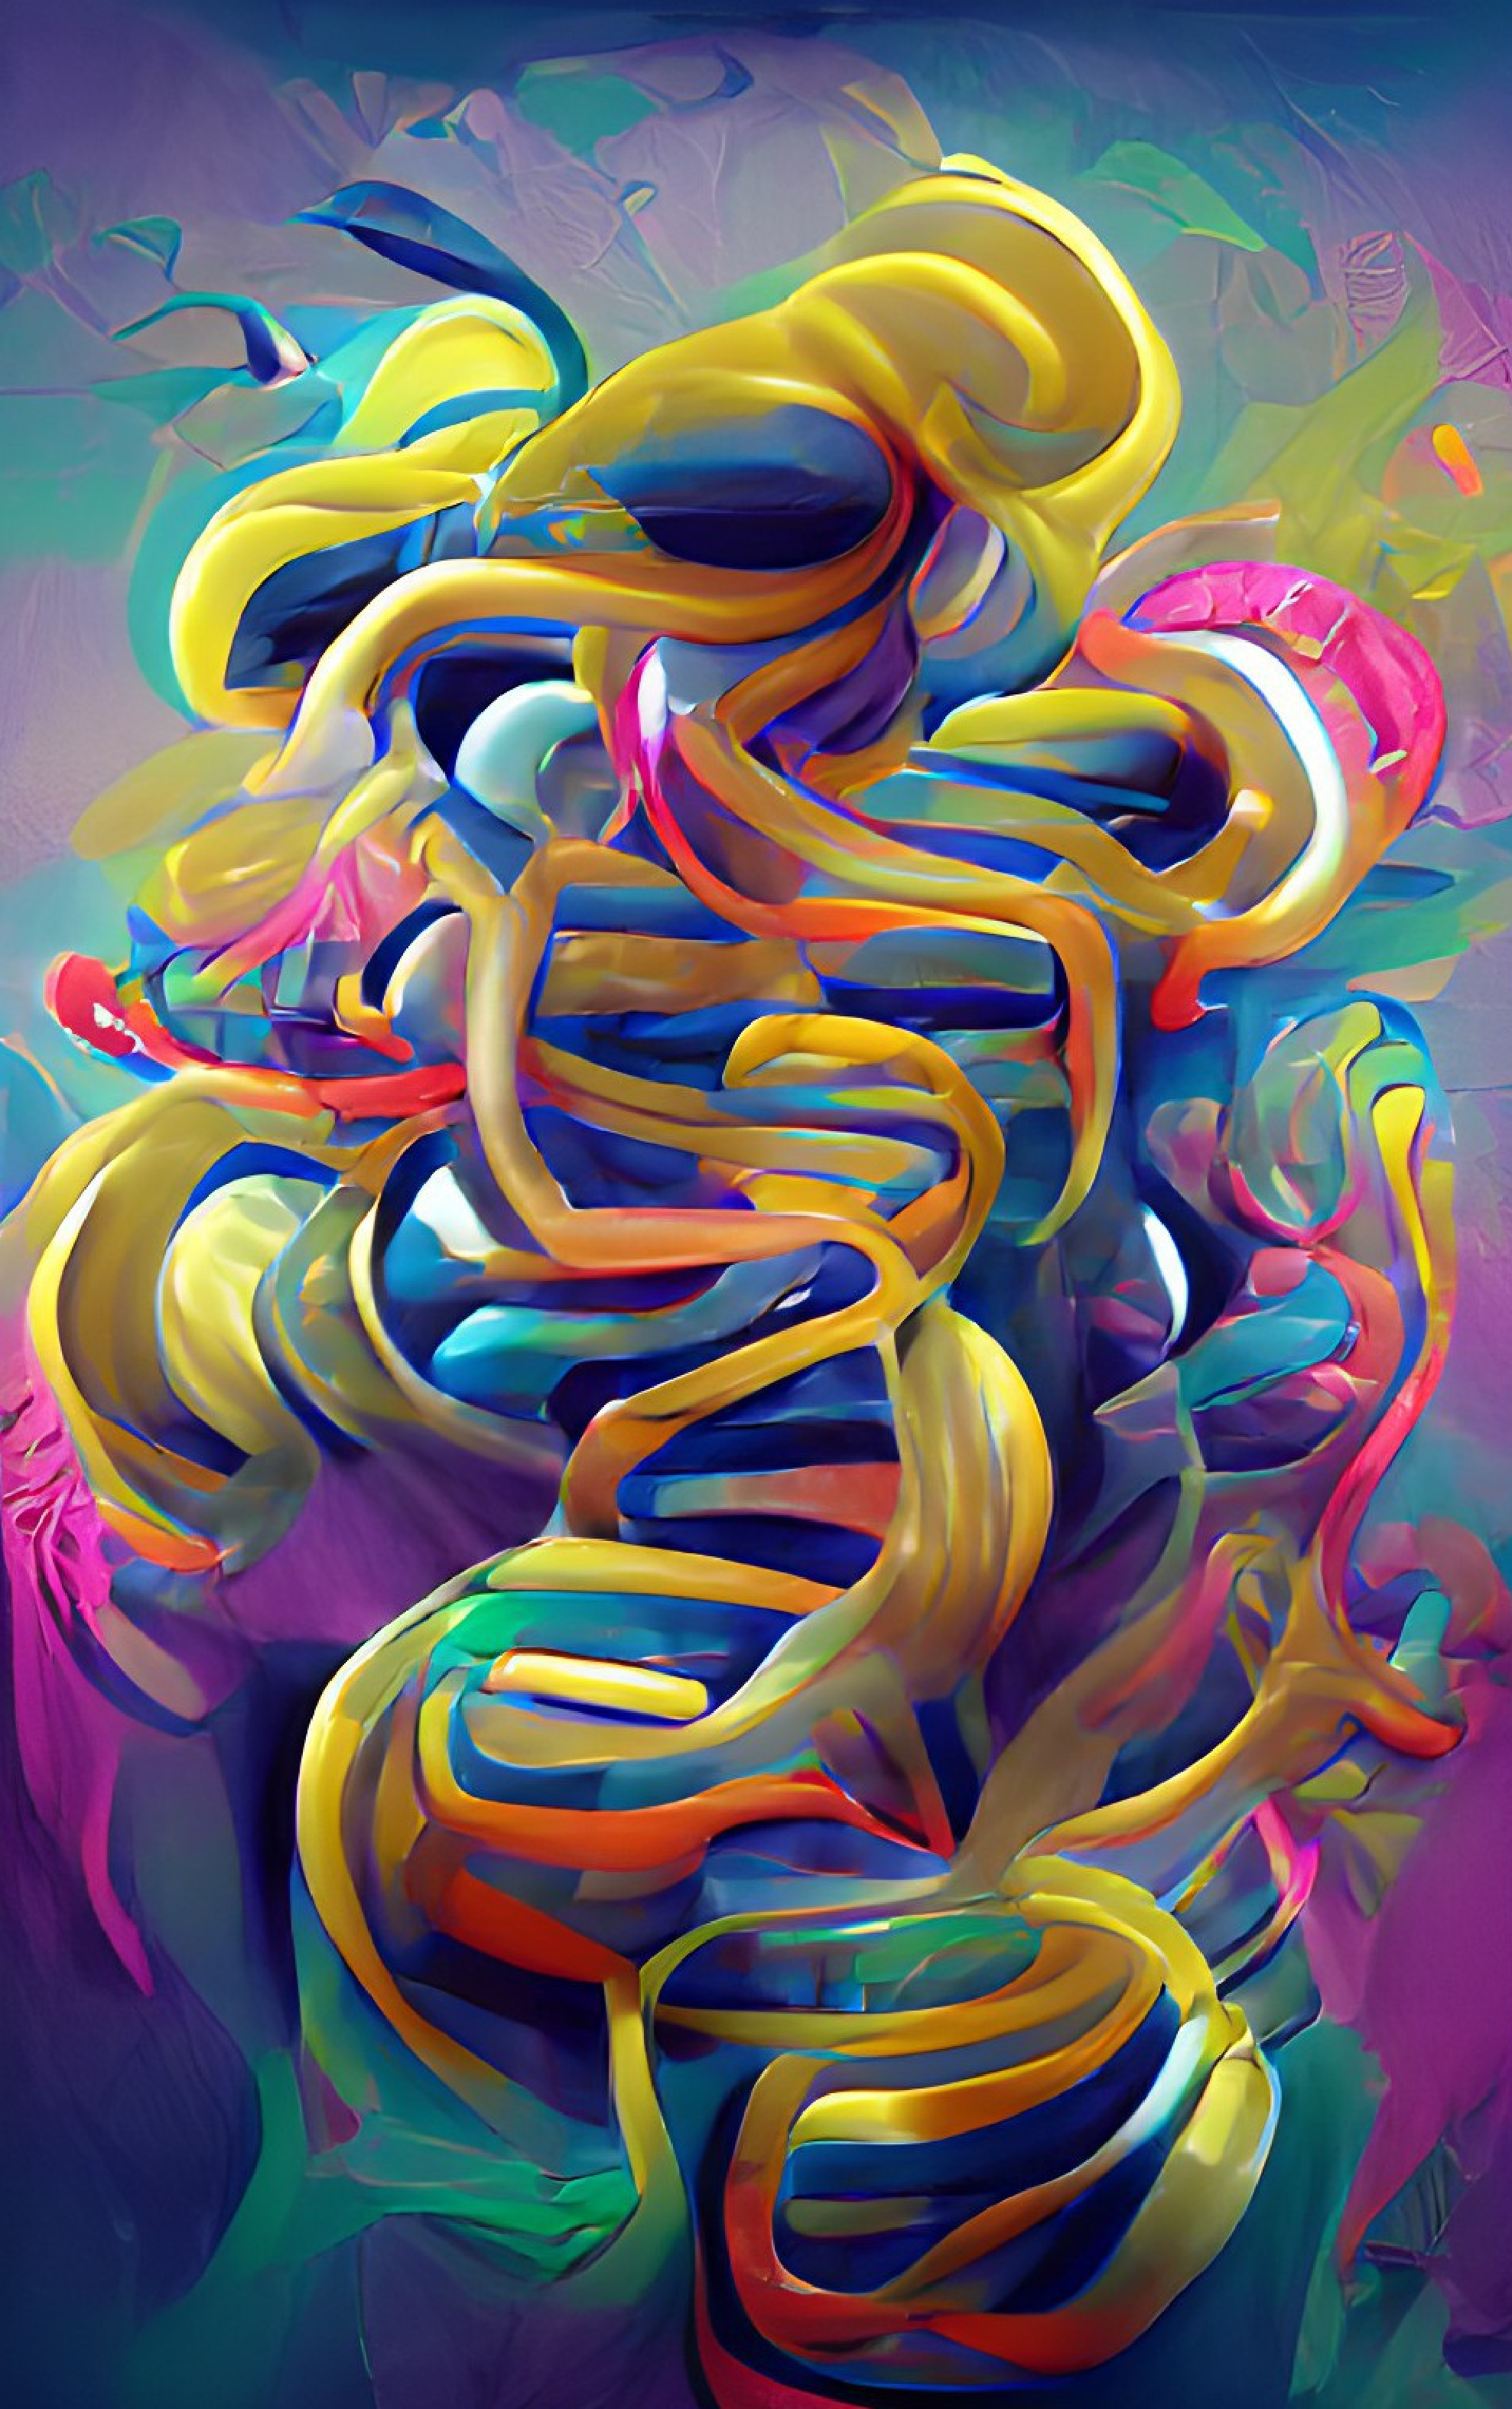
\includegraphics[width=0.5\textwidth]{art.pdf}}

\pagenumbering{roman}

% Begin of the actual contents
\ifadmin
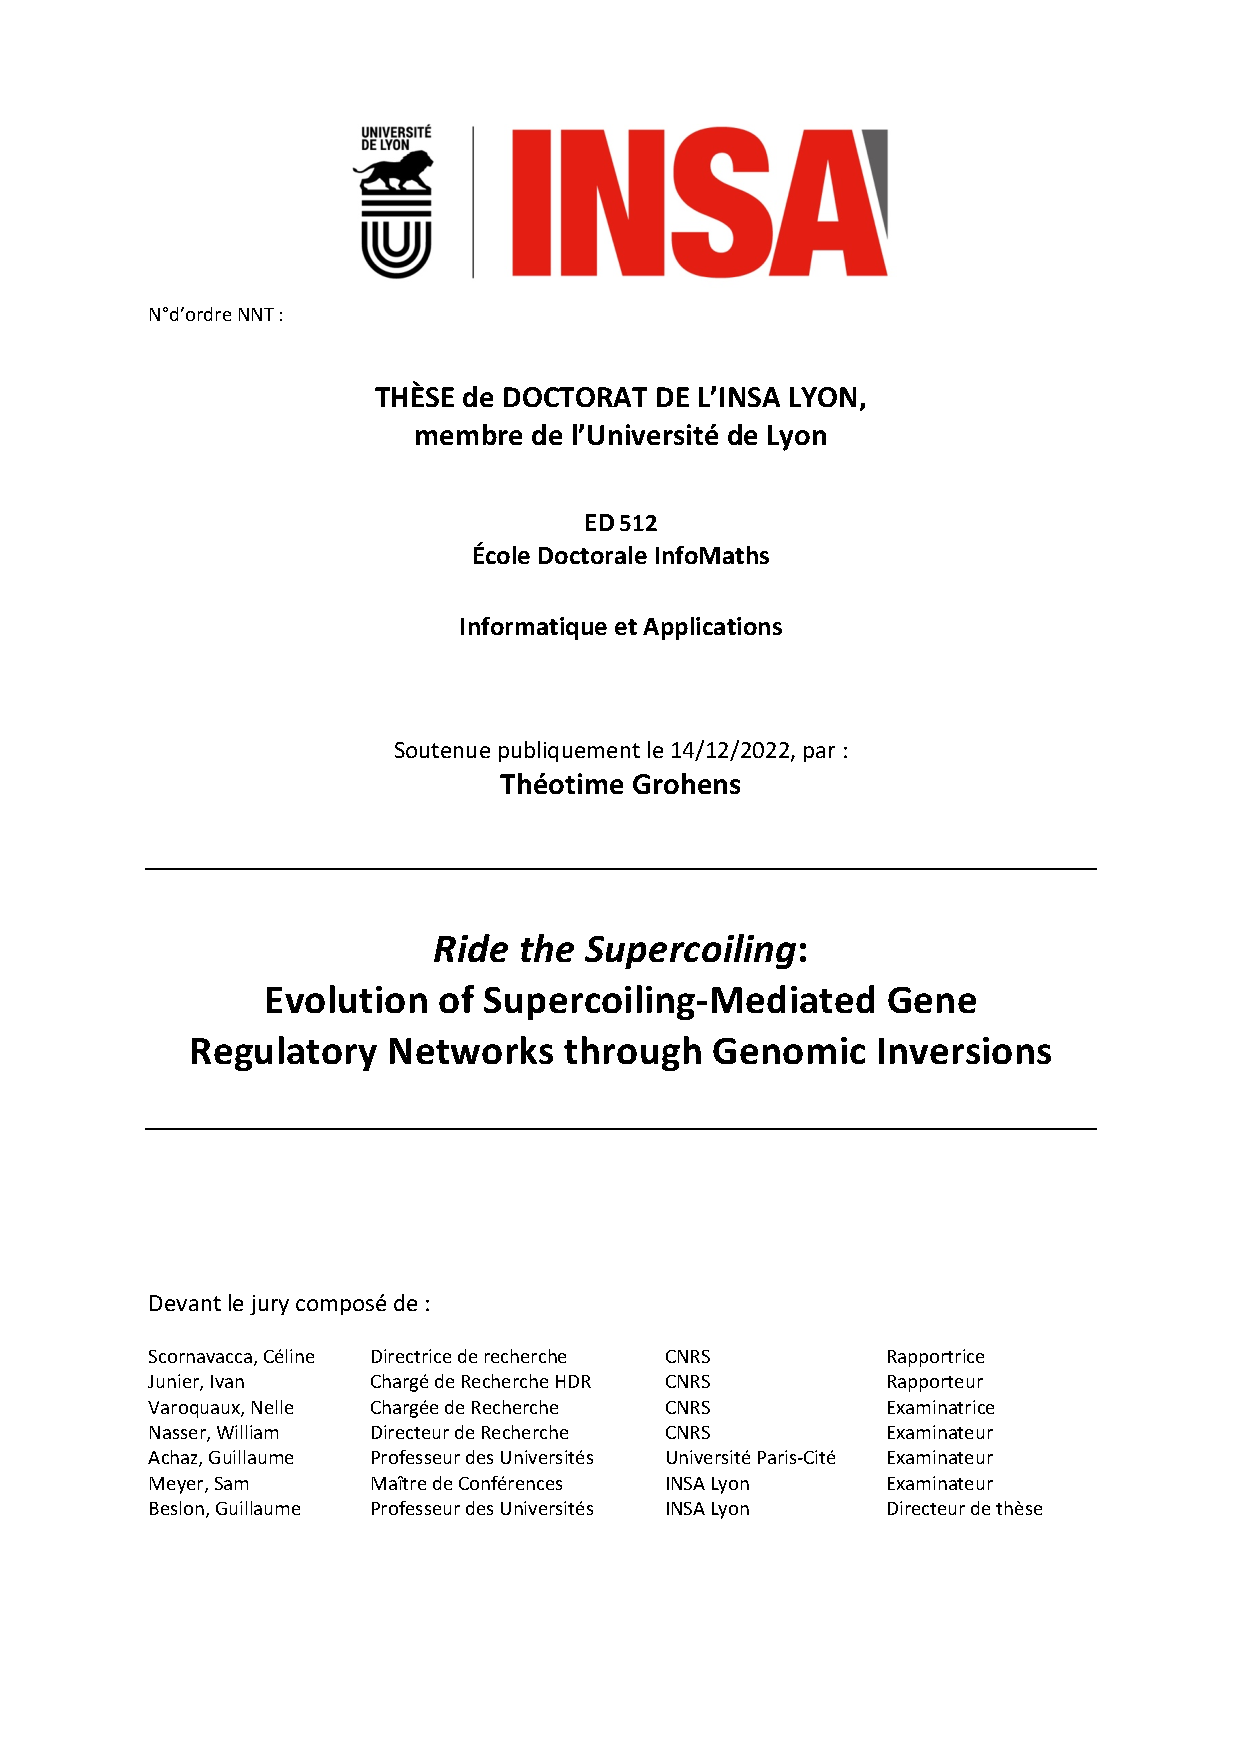
\includepdf{admin/front.pdf}
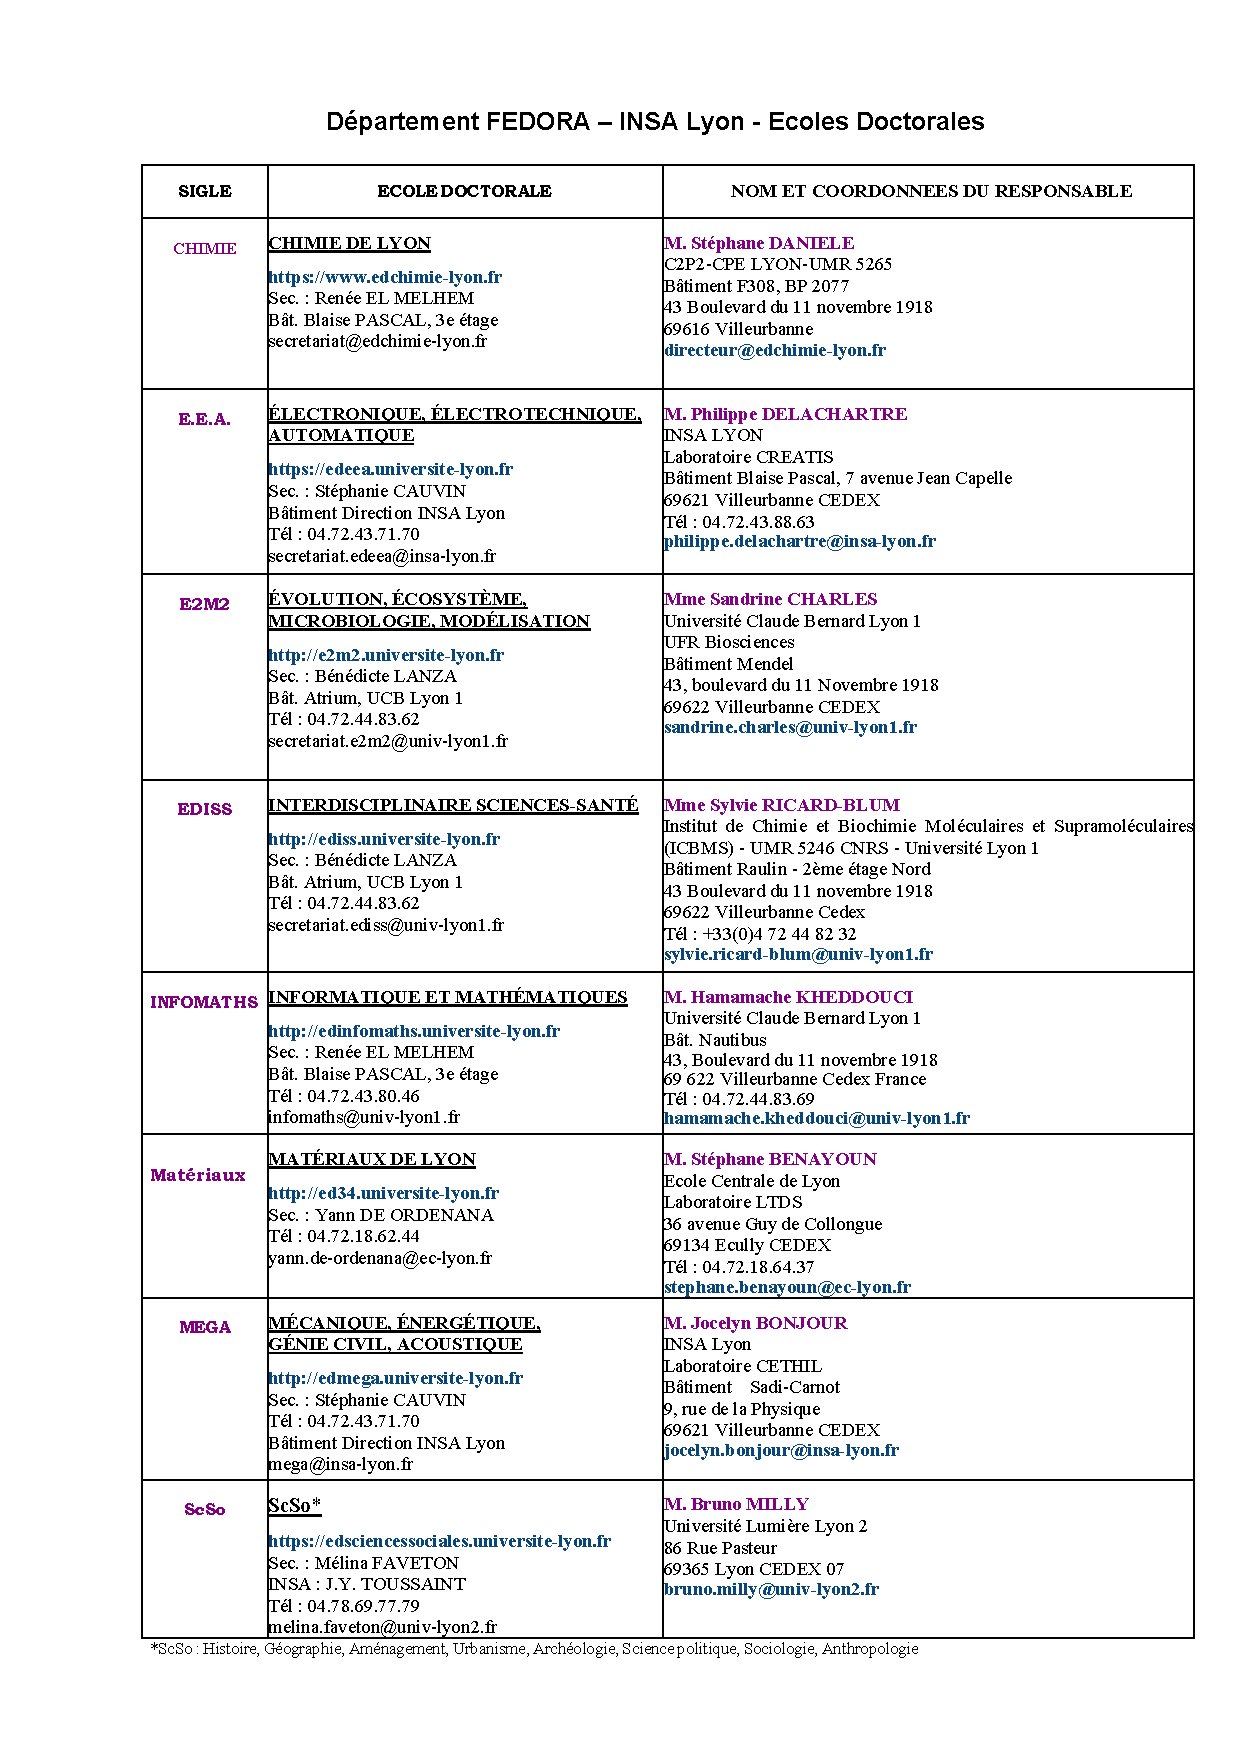
\includepdf{admin/ed.pdf}
\fi

\maketitle
\thispagestyle{empty}
\pagebreak

\frontmatter

\setcounter{page}{1}  % resets the ROMAN page counter to 1

\selectlanguage{french}

\chapter{Résumé en français}
\label{chap:fr-intro}

L'évolution des êtres vivants par sélection naturelle est souvent présentée comme un processus impossible à prédire, car elle trouve sa source dans les mutations aléatoires qui affectent le cœur du vivant, c'est-à-dire la molécule d'ADN, dont la séquence est le support principal de l'information biologique.
Pourtant, s'il n'est pas possible d'identifier avec certitude quelles mutations vont survenir en réponse à une pression de sélection donnée, ni lesquelles parmi celles-ci vont être fixées, de nombreuses expériences laissent penser que le chemin que suit l'évolution n'est pas entièrement dû au hasard.
Cette observation n'est pas nouvelle à l'échelle des organismes macroscopiques : Darwin la faisait déjà dans l'\emph{Origine des Espèces}~\citep{darwin1859}.
Il l'exposa ensuite plus en détail dans la \emph{Variation des animaux et des plantes sous l'action de la domestication}~\citep{darwin1868}, en décrivant de nombreuses plantes et animaux sélectionnés et domestiqués par l'espèce humaine depuis des dizaines de milliers d'années.
Ce caractère répétable est également observable à l'échelle des micro-organismes, avec l'apparition sans cesse renouvelée de résistances aux traitements d'infections bactériennes ou virales~\citep{levy2004}.
Ce n'est toutefois que depuis la fin du XXe siècle, avec le développement du séquençage ADN, que l'on est capable d'essayer de comprendre les soubassements de cette répétabilité, et donc de cette prédictibilité phénotypique, à l'échelle moléculaire.
En effet, on peut désormais observer que c'est parfois le même gène, voire le même nucléotide à l'intérieur d'un gène, qui est touché par des mutations lorsqu'on répète une expérience de sélection pour une caractéristique donnée~\citep{wortel2021}.
Dans ce cas, l'évolution ne semble ainsi plus pouvoir suivre une multitude de chemins différents pour parvenir au même résultat visible, mais semble au contraire contrainte de s'en tenir à un itinéraire bien défini.

L'un des mécanismes qui peuvent expliquer ce caractère répétable de l'évolution est l'épistasie, ou le rôle que joue le contexte génétique sur l'effet d'une mutation donnée.
En effet, il est possible qu'une mutation ait un effet favorable en présence d'une autre mutation, mais un effet défavorable en l'absence de celle-ci.
Ces relations épistatiques peuvent ainsi contraindre les options qui se présentent à l'évolution, en imposant qu'une mutation dans un gène donné survienne avant une autre dans un second gène, afin que la seconde soit favorable.
Dans un contexte de compétition entre souches différentes au sein d'une même population (par exemple, de bactéries pathogènes), mieux comprendre ces relations épistatiques permettrait alors par exemple de prédire plus finement la fixation ou non de futures mutations, et par là la souche victorieuse, offrant la possibilité d'orienter plus finement un traitement.
Le type de relations épistatiques le plus souvent étudié est celui des interactions entre mutations ponctuelles (c'est-à-dire entre mutations n'affectant qu'un seul nucléotide, ou parfois quelques nucléotides contigus) à l'intérieur d'un même gène, car ce sont les mutations les plus faciles à détecter.
Dans ce cas, le changement d'un acide aminé présent à un certain endroit de la protéine codée par le gène peut voir son effet modulé par le changement d'un autre acide aminé de la protéine.
Ces relations épistatiques sont de mieux en mieux comprises, par exemple en mesurant exhaustivement la valeur sélective des $2^N$ mutants possibles pour un groupe de $N$ nucléotides d'intérêt (voir~\cite{achaz2014} pour une vue d'ensemble de telles expériences).
D'autres types d'interactions épistatiques, plus complexes et moins bien étudiés, existent toutefois.
En particulier, il peut y avoir des interactions épistatiques entre différents types de mutations, comme entre mutations locales et réarrangements chromosomiques, ou entre gènes jouant des rôles de natures différentes, par exemple entre un gène codant pour une protéine régulatrice et un autre gène dont l'expression est régulée par cette protéine.
Par exemple, la duplication d'une séquence à l'intérieur d'un gène donné peut être suivie d'une divergence et d'une spécialisation ultérieures de chacune des parties répétées, comme dans la famille des spectrines~\citep{thomas1997}, protéines qui jouent un rôle important dans la structure des cellules eucaryotes.
Il y a alors épistasie entre un réarrangement chromosomique -- la duplication d'une partie d'un gène -- et les mutations ponctuelles qui la suivent : en l'absence de cette duplication, les mutations qui rendent possible la spécialisation des parties dupliquées du gène seraient en effet délétères.

Un cas particulier d'interactions épistatiques est celui des interactions entre les mutations dans les gènes régulant la superhélicité de l'ADN (que j'appellerai mutations de superhélicité) et les mutations dans les gènes eux-mêmes régulés par la superhélicité.
La superhélicité de l'ADN, c'est-à-dire le niveau d'enroulement de l'ADN autour de lui-même, joue en effet un rôle important dans la régulation de la transcription des gènes chez les bactéries, car le niveau de transcription des gènes dépend directement de la superhélicité au niveau de leur promoteur.
L'intérêt évolutif des mutations de superhélicité, ainsi que leur caractère répétable, ont été particulièrement mis en exergue grâce à la \emph{Long Term Evolution Experiment} (\emph{LTEE}) menée dans le laboratoire de Richard Lenski~\citep{lenski1991}.
Dans cette expérience, 12 souches de la bactérie \emph{Escherichia coli} évoluent depuis 1988 dans un environnement de laboratoire et 11 des 12 souches de l'expérience ont vu leur niveau de superhélicité augmenter très tôt au cours de celle-ci, grâce à des mutations touchant un faible nombre de gènes bien identifiés~\citep{crozat2010}.
Comme le niveau de superhélicité est finement régulé par l'activité de plusieurs enzymes (appelées topoisomérases) et par la fixation de protéines sur l'ADN, une mutation dans un gène codant pour l'une ou l'autre de ces protéines peut en effet engendrer un changement de l'activité transcriptionnelle à l'échelle du génome entier.
Les mutations répétées de superhélicité apparaissant dans cette expérience pourraient donc être le signe d'un paysage d'interactions épistatiques biaisé, qui augmenterait la proportion de mutations favorables pouvant apparaître dans les génomes qui les contiennent, rendant par là plus probable le futur succès évolutif de leur lignée.

Le questionnement majeur sous-tendant les travaux que j'ai menés pendant ma thèse a donc été de déterminer à quel point la présence ou non de mutations de superhélicité dans une lignée permet de prédire le futur succès de celle-ci, afin de comprendre plus généralement l'influence des biais épistatiques dans la répétabilité et la prédictibilité de l'évolution.
Pour cela, j'ai étudié le rôle évolutif des mutations de superhélicité au cours de l'adaptation à un nouvel environnement, en employant une approche d'évolution expérimentale \emph{in silico}, qui s'inscrit dans le cadre plus large de la biologie évolutive des systèmes~\citep{beslon2021}.
J'ai commencé par intégrer un modèle d'expression des gènes prenant en compte le niveau de superhélicité à l'échelle du chromosome dans un logiciel de simulation d'évolution existant au sein de mon équipe de thèse, le logiciel \emph{Aevol}.
Ce modèle et les premiers résultats obtenus à l'aide de celui-ci sont présentés dans le chapitre~\ref{chap:aevol} de la thèse.
Les expériences menées dans ce cadre ont permis d'obtenir un résultat évolutif qualitativement semblable à celui de la \emph{LTEE}, la superhélicité étant la cible de nombreuses mutations au début de l'évolution.
Toutefois, celle-ci se stabilise rapidement alors même que le reste du génome des individus continue d'évoluer, ne permettant pas de conclure sur de possibles interactions épistatiques.

Or, le rôle que tient le niveau de superhélicité de l'ADN dans la régulation de l'expression des gènes bactériens provient en réalité de son caractère extrêmement dynamique~\citep{martisb.2019}.
Ce caractère dynamique de la superhélicité, tant dans le temps que le long du génome, est en particulier dû à la transcription elle-même des gènes~\citep{visser2022}.
En effet, d'après un modèle initialement proposé par~\cite{liu1987}, lorsqu'un gène est en cours de transcription par une ARN polymérase, l'encombrant complexe qui en résulte ne peut pivoter autour de l'ADN aussi vite que l'ADN s'enroule autour de lui-même.
Le couple ainsi exercé sur l'ADN provoque alors une accumulation de superhélicité en avant du gène transcrit et un déficit de superhélicité en arrière de celui-ci.
La transcription d'un gène donné peut donc influer -- par l'intermédiaire des changements locaux de superhélicité qu'elle engendre -- sur la transcription des gènes à proximité de celui-ci et ainsi créer un réseau d'interactions entre les niveaux d'expressions de gènes proches sur le génome.
Une modélisation de la superhélicité prenant en compte les variations locales de celle-ci dues à la transcription semble donc pertinente pour l'étude du rôle évolutif des mutations de superhélicité.
Une approche aussi précise s'étant révélée délicate à mettre en place dans \emph{Aevol}, j'ai opté pour la création d'un nouveau modèle représentant plus abstraitement le génome, mais décrivant plus fidèlement le couplage entre superhélicité et transcription.
J'ai implémenté ce nouveau modèle -- appelé \emph{EvoTSC} -- en Python.
Le code de celui-ci est disponible à l'adresse suivante : \url{https://gitlab.inria.fr/tgrohens/evotsc}.

À l'aide d'\emph{EvoTSC}, j'ai dans un premier temps montré que, dans un modèle où le seul mécanisme de régulation de l'activité des gènes est le couplage médié par la superhélicité entre les niveaux de transcription de gènes proches, et où les seules mutations possibles sont les inversions chromosomiques (qui réorganisent les positions relatives des gènes), il est possible d'obtenir par sélection naturelle des individus dont les gènes atteignent avec précision des niveaux d'expression optimaux dépendant de l'environnement.
En particulier, il est possible d'obtenir des gènes activés par une relaxation globale de l'ADN, alors que leurs promoteurs sont intrinsèquement inhibés par la relaxation de l'ADN.
Ces premiers résultats sont présentés dans le chapitre~\ref{chap:alife}.
Ils démontrent que la superhélicité peut jouer un rôle majeur dans la régulation de l'activité des gènes bactériens en permettant l'existence de réseaux de régulation génétique même en l'absence de facteurs de transcription.
Ils ont été publiés, d'abord sous forme d'article dans la conférence \emph{ALIFE 2021}~\citep{grohens2021}, puis dans une version étendue dans le journal associé, \emph{Artificial Life}~\citep{grohens2022a}.

Dans un second temps, j'ai cherché à caractériser plus en détail l'impact évolutif de la superhélicité sur la structure des génomes et des réseaux de régulations bactériens.
Toujours en utilisant le modèle \emph{EvoTSC}, j'ai montré qu'au niveau le plus local, des paires convergentes ou divergentes de gènes voisins se forment, conformément aux prédictions théoriques du couplage entre superhélicité et transcription.
J'ai montré que cette organisation à l'échelle locale du génome n'était toutefois pas entièrement suffisante pour expliquer les niveaux d'expression des gènes observés dans le génome complet, mais que des sous-réseaux impliquant jusqu'à plusieurs dizaines de gènes peuvent au contraire être nécessaires.
Enfin, en utilisant une approche par knock-out de gène, j'ai montré que, dans le génome des individus évolués, c'est sous la forme d'un réseau unique et s'étendant à l'échelle du génome entier que s'organise la régulation de l'expression des gènes dans le modèle \emph{EvoTSC}.
Ce second ensemble de résultats est présenté dans le chapitre~\ref{chap:ploscb} et a été mis en forme dans une prépublication qui sera prochainement soumise à relecture par les pairs~\citep{grohens2022b}.

Dans le chapitre~\ref{chap:param}, je présente ensuite un ensemble d'expériences complémentaires qui montrent la robustesse des résultats du modèle \emph{EvoTSC} présentés dans les chapitres précédents, en réponse à des variations des principaux paramètres du modèle visant à représenter la diversité des génomes bactériens et des changements environnementaux.
J'ai finalement incorporé dans \emph{EvoTSC} un modèle d'évolution du niveau de superhélicité globale, afin de pouvoir caractériser, de la même manière que dans les expériences menées avec \emph{Aevol}, les possibles relations épistatiques entre mutations de superhélicité et réarrangements chromosomiques.
Je me suis en particulier intéressé à l'étude des paysages adaptatifs (\emph{fitness landscapes}) résultant des mutations de superhélicité.
Ces résultats sont présentés dans le chapitre~\ref{chap:epistasis} et ouvrent la voie à la conclusion de ce manuscrit au chapitre~\ref{chap:conclusion}.

\paragraph{}
L'annexe~\ref{chap:software} présente les contributions logicielles que j'ai réalisées tout au long de ma thèse.
J'ai d'abord participé au développement d'\emph{Aevol} et d'outils associés pour gérer des simulations et analyser les résultats obtenus avec celles-ci.
Ensuite, j'ai développé le modèle \emph{EvoTSC}, ainsi qu'un ensemble d'outils pour visualiser et analyser les données produites par le modèle.

Pour finir, l'irruption de la pandémie de Covid-19 en France au printemps 2020 a perturbé le cours de ma thèse d'une manière particulière.
Je me suis en effet porté volontaire pour participer à une collaboration entre l'Assistance Publique-Hôpitaux de Paris (AP-HP) et un groupe de chercheur·ses et d'ingénieur·es Inria constitué à cet effet.
Avec l'accord de mon directeur de thèse, j'ai alors interrompu mes travaux sur la superhélicité pour me consacrer pleinement à cet effort pendant plusieurs semaines en avril et mai 2020.
Dans ce cadre, j'ai participé à la construction d'un modèle de l'épidémie de Covid-19 dans l'agglomération parisienne, visant à aider les équipes de l'AP-HP à suivre en temps réel -- et essayer de prédire -- l'évolution de cette épidémie à l'aide de données de régulation médicale.
Ces travaux ont par la suite mené à une publication~\citep{gaubert2020}, présentée dans l'annexe~\ref{chap:covid}.

\selectlanguage{english}


\renewcommand*{\contentsname}{Table of Contents}

\tableofcontents
\listoffigures
\listoftables

\mainmatter

\chapter{Introduction}
\label{chap:intro}

The evolution of living things by natural selection is often presented as an unpredictable process, because it originates in the random mutations that affect the core of living things: the DNA molecule, whose sequence is the main carrier of biological information.
However, while it is not possible to identify with certainty which specific mutations will occur in response to a given selection pressure, many experiments suggest that the path that evolution follows is not entirely random and may even be reproducible.
This may seem obvious at the scale of organisms, thinking of the many plants and animals selected and domesticated by the human species over tens of thousands of years, or the repeated appearance of resistance to treatments for bacterial or viral infections.
However, it is only since the 20th century that we have been able to try to understand the basis of this repeatability at the molecular level.
We then observed that it is sometimes the same gene, or even the same nucleotide within a gene, that is affected by mutations when a selection experiment is repeated for a given characteristic.
In this case, evolution no longer seems to be able to follow a multitude of different paths to reach the same visible result, but is forced to stick to a well-defined route.

One mechanism that may explain this repeatability of evolution is epistasis, or the role that the genetic environment plays in the effect of a given mutation.
Indeed, it is possible for a mutation to have a favorable effect in the presence of another mutation, but an unfavorable effect in the absence of it.
These epistatic relationships can thus constrain the options available to evolution, by requiring that a mutation of a given gene occur before that of a second gene, in order for the latter to be favorable.
In a context of competition between different strains within the same population (for example, of pathogenic bacteria), a better understanding of these epistatic relationships would then allow, for example, a more accurate prediction of the fixation or not of future mutations, and thus of the victorious strain, offering the possibility of more accurately orienting a treatment.
The type of epistatic relationships most often studied is that of interactions between point mutations, i.e. between mutations affecting only a small number of contiguous nucleotides within the same gene, as these are the easiest mutations to detect.
However, there are many other types of epistatic interactions that are more complex and less well studied.
For example, the duplication of a gene followed by a divergence and specialization of its two copies in two different functions, a process that plays a major role in innovation at the molecular level, can be interpreted in this context.
There is then an epistasis between a chromosomal rearrangement, the duplication of a gene and the subsequent point mutations; in the absence of this duplication, the mutations which make possible the specialization of the copies of the gene would indeed be deleterious. \textbf{Is the example really necessary?}

The starting point of my thesis was therefore the study of a particular case of epistatic interactions, those generated by mutations in genes regulating DNA supercoiling.
DNA supercoiling, or the degree to which DNA is wrapped around itself, plays an important role in the regulation of gene activity in bacteria, because the level of gene transcription depends directly on the supercoiling at the promoter.
As the level of supercoiling is finely regulated by the activity of several enzymes, called topoisomerases, a mutation in a gene coding for one of these can lead to a change in transcriptional activity at the scale of the entire genome,
This opens the door to the emergence of numerous compensatory mutations.
The evolutionary role of supercoiling mutations, and their repeatability, has been highlighted in particular in the \emph{Long Term Evolution Experiment} carried out in the laboratory of Richard Lenski, which has been evolving 12 strains of \emph{Escherichia coli} in a laboratory environment since 1988.
Indeed, 11 of the 12 strains have seen their supercoiling increase very early in the course of the experiment.

To address the study of the evolutionary role of these mutations during adaptation to a new environment, I opted for an evolutionary systems biology approach.
I started by integrating a gene expression model taking into account the level of supercoiling at the chromosome level in an evolutionary simulation software existing within my thesis team, the software \emph{Aevol}.
This model, and the first results obtained with it, are presented in chapter~\ref{chap:aevol} of the thesis.
However, the experiments carried out in this framework did not lead to a convincing result, the supercoiling converging very quickly during the evolution to a constant level, while the rest of the genome of the individuals continues to evolve.

The role in the regulation of gene expression that the level of supercoiling in bacterial DNA holds actually comes from the highly dynamic nature of supercoiling, which is largely related to gene transcription. \textbf{??}
When a gene is transcribed by an RNA polymerase, the resulting bulky enzyme complex is unable to turn around the DNA as fast as the DNA turns around itself, resulting in an accumulation of supercoiling downstream of the gene, and a deficit of supercoiling upstream of it.
The transcription of a given gene can thus influence, through the changes in supercoiling in its vicinity that it generates, the transcription of genes in its vicinity, thus creating a network of interactions and couplings between the expression levels of nearby genes on the genome.
As such a detailed modeling of supercoiling was difficult to implement in the model \emph{Aevol}, I opted to study, in a first step, its evolutionary role in a model integrating a simplified genome, but describing more accurately supercoiling.
I implemented this model, called \emph{EvoTSC}, from scratch in Python, and it is available at \url{https://gitlab.inria.fr/tgrohens/evotsc}.

Using \emph{EvoTSC}, I first showed that, in a model where the only mechanism for regulating gene activity is supercoiling-mediated coupling between the transcript levels of nearby genes, and where the only possible mutations are chromosomal inversions (which rearrange the relative positions of the genes), it is possible to obtain by natural selection individuals whose genes accurately follow environment-dependent targets.
In particular, it is possible to obtain genes that are activated by global DNA relaxation, while their promoters are inhibited by local relaxation.
These first results are presented in the chapter~\ref{chap:alife}, and demonstrate that supercoiling can indeed play a major role in the regulation of bacterial gene activity, as a support of a genetic regulation network.
They were published, first as a paper in the conference \emph{ALIFE 2021}~\citep{grohens2021}, and then in an extended version in the associated journal, \emph{Artificial Life}~\citep{grohens2022a}.

In a second step, I then sought to characterize in more detail the evolutionary impact of supercoiling in the structure of bacterial genomes.
Still using the \emph{EvoTSC} model, I showed that at the most local level, convergent or divergent pairs of neighboring genes are formed, in accordance with theoretical predictions of the coupling between supercoiling and transcription.
I have shown that this organization at the local genome scale is, however, not entirely sufficient to explain the gene expression levels observed in the whole genome, but that subnetworks involving up to several tens of genes may instead be required.
Finally, using a gene knockout approach, I have shown that in the genomes of evolved individuals, it is in the form of a single, genome-wide network that the regulation of gene expression is organized in the EvoTSC model.
This second set of results is presented in chapter~\ref{chap:ploscb}, and has been formatted in a pre-publication~\citep{grohens2022b}, soon to be submitted for peer review.

In chapter~\ref{chap:param}, I then present a set of complementary experiments that show the robustness of the model results \emph{EvoTSC} presented so far, when varying the main parameters of the model.
Finally, I have incorporated in EvoTSC a model of the evolution of the global supercoiling level, in order to characterize, as in the experiments conducted with Aevol, the possible epistatic relationships between supercoiling mutations and chromosomal rearrangements.
These results are presented in the chapter~\ref{chap:epistasis}.

The appendix~\ref{chap:software} presents the software contributions I made throughout my thesis.
I first participated in the development of \emph{Aevol} and associated tools to manage simulations, then developed the \emph{EvoTSC} model as well as a set of tools to visualize and analyze the resulting data.

Finally, the course of my thesis having been disrupted by the outbreak of the Covid-19 pandemic in France in the spring of 2020, I volunteered to collaborate, within a team of Inria researchers and engineers, with the Assistance Publique-Hôpitaux de Paris (AP-HP).
Together we built a model of the epidemic in the Parisian agglomeration, which aimed to help the AP-HP teams to follow in real time and try to predict the evolution of the epidemic using medical regulation data.
This work subsequently led to a publication~\citep{gaubert2020}, presented in Appendix~\ref{chap:covid}.

\selectlanguage{english}

\chapter{Background}
\label{chap:background}

In this chapter, I introduce the biological concepts and methods that will be used throughout this manuscript.
I first present DNA supercoiling and its regulation in bacteria.
I outline its role in gene transcription, and the reciprocal effect of transcription on supercoiling, which jointly result in what is called the transcription-supercoiling coupling (TSC).
Then, I discuss a few cases studies in which supercoiling might have played an important evolutionary role, and that illustrate the interest of studying DNA supercoiling through the lens of evolution.
Finally, I briefly present the general method with which I tackle the questions raised in Chapter~\ref{chap:intro} throughout the manuscript.

\section{DNA Supercoiling in Bacteria}
\label{sec:background:sc}

\begin{figure}
  \centering
  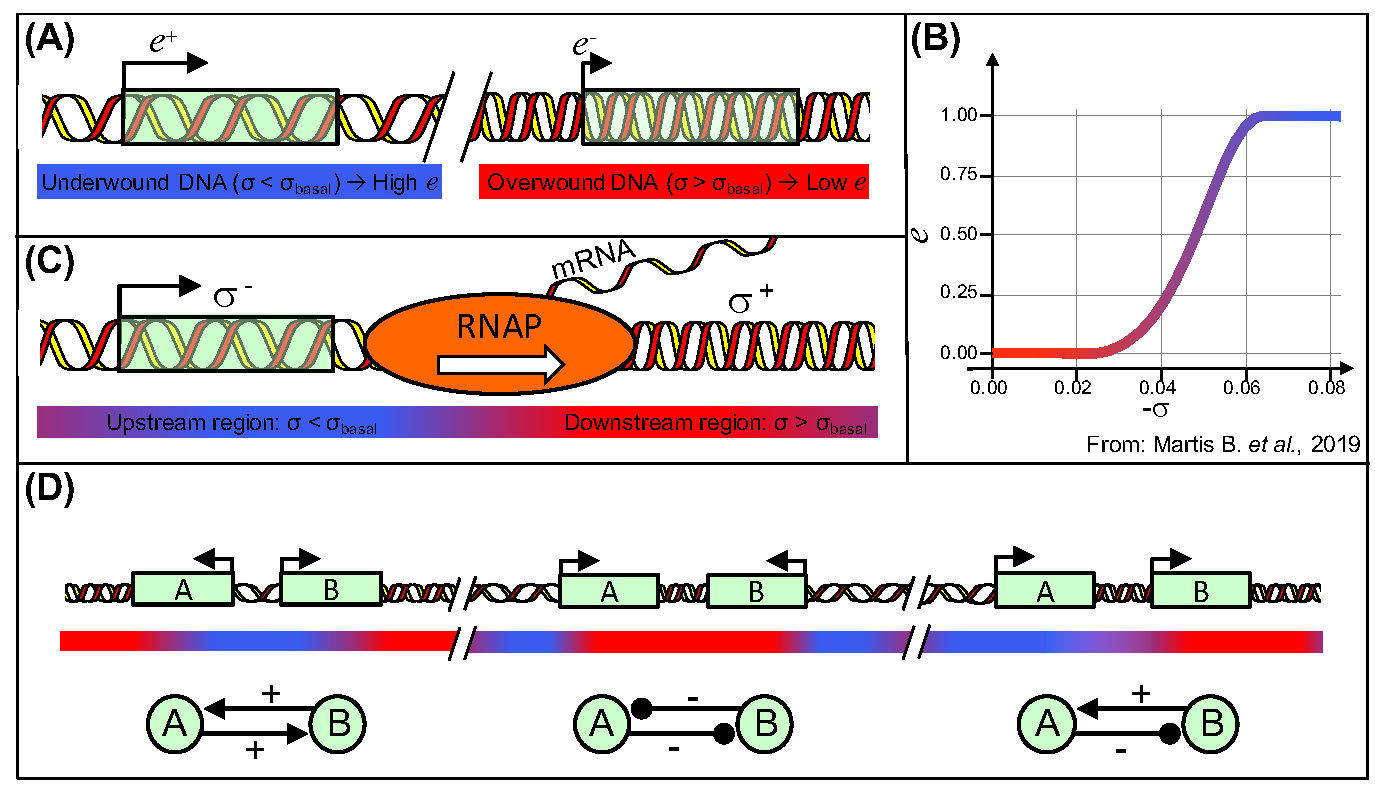
\includegraphics[width=\textwidth]{alife/img/fig-theorique.pdf}
  \caption[Role of supercoiling in transcription and description of the transcription"=supercoiling coupling]{\textbf{A}. When DNA is underwound ($\sigma < \sigma_{basal}$, left), gene transcription rates are higher than when DNA is overwound ($\sigma > \sigma_{basal}$, right).
  \textbf{B}. Promoter activity (equivalently, transcription level) \emph{e} increases with the level of negative supercoiling $-\sigma$.
  \textbf{C}. The transcription of a gene by RNA polymerase (RNAP) generates a decrease in supercoiling upstream of the transcribed gene, and an increase downstream of the transcribed gene.
  \textbf{D}. Transcription-supercoiling coupling: the sign of the interaction between neighboring genes depends on their relative orientation.
  Figure reproduced from~\citep{grohens2021}.}
  \label{fig:background:theory}
\end{figure}

%\paragraph{Definition of DNA supercoiling}
DNA is the material basis of genetic information.
It is a flexible polymer that comprises two strands of nucleotides that coil around each other, at a rate of 10.5 base pairs per turn in the absence of external constraints.
When subjected to torsional stress, DNA can either writhe and form 3-dimensional loops, or twist around itself more or less tightly than in its relaxed state~\citep{travers2005}; both writhing and twisting are referred to as DNA supercoiling.
The level of supercoiling is measured as the relative density $\sigma$ of supercoils in over- or under-wound DNA, as compared to relaxed DNA.
DNA is positively supercoiled ($\sigma > 0$) when it is overwound, and negatively supercoiled ($\sigma < 0$) when it is underwound.
In bacteria, DNA is normally maintained in a moderately negatively supercoiled state, with a reference value of $\sigma_{basal}=-0.06$ in \emph{Escherichia coli}~\citep{travers2005}.
In these organisms, the supercoiling level is an important regulator of gene transcription~\citep{dorman2016}.
Moreover, as transcription itself impacts DNA supercoiling~\citep{liu1987}, this results in a coupling between these two processes, of which Figure~\ref{fig:background:theory} presents an overview.
As a general rule, genes are transcribed at a higher rate when DNA is more negatively supercoiled (A), following a sigmoidal response curve (B).
Transcription generates positive and negative supercoiling downstream and upstream of transcribed genes respectively (C), resulting in a coupling between the expression levels of neighboring genes that depends on their relative orientations (D).

\subsection{Gene Regulation by DNA Supercoiling}

The level of DNA supercoiling influences gene expression, as more negatively supercoiled DNA facilitates the initiation of transcription (Figure~\ref{fig:background:theory} A).
The thermodynamical reaction of opening the DNA double strand, which is the initial step of gene transcription, is indeed favored in more negatively supercoiled DNA~\citep{elhoudaigui2019}, resulting in a sigmoidal response curve of gene expression to DNA supercoiling (Figure~\ref{fig:background:theory} B).

Due to this effect, supercoiling has experimentally been shown to act as a broad regulator of gene expression in several bacteria.
In \emph{E. coli},~\cite{peter2004} showed that 7\% of genes were sensitive to a relaxation of chromosomal DNA, of which one third were up-regulated by relaxation and two thirds down-regulated.
Similar results were obtained for \emph{S. enterica}, in which 10\% of genes were sensitive to DNA relaxation~\citep{webber2013}, and for \emph{S. pneumoniae}, in which around 13\% of genes were sensitive to relaxation~\citep{ferrandiz2010}.
When instead inducing extreme negative supercoiling in \emph{D. dadantii}, 13\% of the genes in the exponential phase and 7\% in the stationary phase were affected~\citep{pineau2022a}.

In \emph{D. dadantii}, different genomic regions moreover exhibit markedly different responses to changes in supercoiling~\citep{muskhelishvili2019}, allowing the expression of pathogenic genes only in stressful environments.
Finally, DNA supercoiling might be an especially important regulator of gene activity in bacteria with reduced genomes, such as the obligate aphid endosymbiotic bacterium \emph{Buchnera aphidicola}.
\emph{B. aphidicola} is nearly devoid of transcription factors, and supercoiling is therefore though to be one of the sole regulation mechanisms available in this bacteria~\citep{brinza2013}.

\subsection{A Dynamic DNA Supercoiling Level}

The level of DNA supercoiling in bacteria is primarily controlled by topoisomerases, enzymes that alter DNA supercoiling by cutting and rotating the DNA strands~\citep{duprey2021}.
The two main topoisomerases are gyrase, which dissipates positive supercoiling by introducing negative supercoils at an ATP-dependent rate, and topoisomerase I, which oppositely relaxes negative supercoiling~\citep{martisb.2019}.
But numerous other processes also impact the level of DNA supercoiling, either by generating new supercoils or by constraining their diffusion.

In particular, according to the twin-domain model of supercoiling~\citep{liu1987}, the transcription of a gene by RNA polymerase generates both positive and negative supercoils.
As a consequence of the drag that hampers the rotation of the RNA polymerase complex around the DNA sequence during transcription, positive supercoiling builds up upstream of the transcribed gene, and negative supercoiling downstream of the transcribed gene~\citep{visser2022}.
This phenomenon is pictured in subfigure C of Figure~\ref{fig:background:theory}.
Moreover, while the intrinsic flexibility of the DNA polymer would in principle allow supercoils to propagate freely along the chromosome, many nucleoid-associated proteins such as FIS, H-NS or HU bind to bacterial DNA~\citep{krogh2018}, in addition to RNA polymerases.
These DNA-bound proteins create barriers that block the diffusion of supercoils, resulting in what have been termed topological domains of supercoiling~\citep{postow2004}.

The level of DNA supercoiling can furthermore be affected by numerous environmental stresses in bacteria.
Salt shock transiently increases negative DNA supercoiling in \emph{E. coli}~\citep{hsieh1991}; the acidic intracellular environment relaxes DNA in the facultative pathogen \emph{Salmonella enterica} var. Typhimurium~\citep{marshall2000}; and higher temperatures relax DNA in the plant pathogen \emph{Dickeya dadantii}~\citep{herault2014}.
These constraints overall paint the picture of a very dynamic DNA ``supercoiling landscape'' in bacteria~\citep{visser2022}, with a supercoiling level that varies in both time and space during the bacterial lifecycle and along the chromosome.

\subsection{Supercoiling and Evolution}

Gene regulation by DNA supercoiling can itself be subject to evolution by natural selection, as a mechanism by which to adapt gene expression levels to new environments.
In the \emph{Long-Term Evolution Experiment} (\emph{LTEE})~\citep{lenski1991}, 12 populations of \emph{E. coli} have been maintained for over 80,000 generations, evolving and adapting to a glucose-limited environment.
In 11 of the 12 populations in the experiment, an increase in fitness was linked to mutations in genes which participate directly or indirectly in the regulation of the supercoiling level, such as \emph{topA}, \emph{fis}, or \emph{dusB}~\citep{crozat2010}.
When inserted into the ancestral strain, the mutant \emph{topA} and \emph{fis} alleles increased the level of negative supercoiling as well as the bacterial growth rate, demonstrating
that supercoiling mutations can play a role in the adaptation to new environments through their broad regulatory effect~\citep{crozat2005}.
From an epistasis perspective, the repeated fixation of supercoiling mutations in the \emph{LTEE} suggests that these mutations could confer an evolutionary advantage to the lineages in which they appear by favoring the apparition of compensatory mutations in supercoiling-regulated genes; but this possible epistatic role should nonetheless be disentangled from their direct fitness effect in order to conclude with more certainty.

The regulation of gene expression by DNA supercoiling could moreover be a force that participates in shaping the evolution of the organization itself of bacterial genomes.
Indeed, supercoiling"=sensitive genes tend to group in up or down-regulated clusters in \emph{E. coli}~\citep{peter2004}, \emph{S. enterica}~\citep{webber2013} and \emph{S. pneumoniae}~\citep{ferrandiz2010}.
This suggests the possibility of a phenotypic role in the co-localization of genes in these clusters, through a common regulation of their transcription~\citep{sobetzko2016}.
Synteny segments, or clusters of neighboring genes that show correlated expression patterns, are indeed evolutionarily conserved across \emph{E. coli} and the distantly related \emph{Bacillus subtilis}, strengthening the hypothesis that these domains could play an important role in the regulation of bacterial gene expression through supercoiling-mediated interactions~\citep{junier2016}.


\section{The Transcription-Supercoiling Coupling}

As shown in Figure~\ref{fig:background:theory}C, the transcription of a given gene by an RNA polymerase generates an accumulation of positive supercoiling downstream of that gene, and of negative supercoiling upstream of that gene, because of the hindered movement of the polymerase~\citep{liu1987,visser2022}.
If a second gene is located closely enough to this first gene on the genome, the change in supercoiling at the promoter of the second gene will impact the transcription rate of that gene, as negative supercoiling usually facilitates gene transcription~\citep{forquet2021}.
In turn, the transcription of the second gene will also generate a local change in supercoiling that affects the first gene, resulting in an interaction between the transcription levels of these two genes, which has been called the transcription-supercoiling coupling~\citep{meyer2014}.
Depending on the relative orientation of these genes, the coupling can take several forms.
Divergent genes increase their respective transcription level in a positive feedback loop; convergent genes inhibit the transcription of one another; and in tandem genes, the transcription of the downstream gene increases the transcription of the upstream gene, while the transcription of the upstream gene decreases the transcription of the downstream gene.

This supercoiling-mediated interaction between neighboring genes has been documented in several bacterial genetic systems.
In the \emph{E. coli}-related pathogen \emph{Shigella flexneri}, the \emph{virB} promoter is normally only active at high temperature, but can be activated at low temperature by the insertion of a phage promoter in divergent orientation~\citep{tobe1995}.
Similarly, the expression of the \emph{leu-500} promoter in \emph{S. enterica} can be increased or decreased by the insertion of upstream transcriptionally active promoters, depending on their orientation relative to \emph{leu-500}~\citep{elhanafi2000}.
The magnitude of the effect of the transcription-supercoiling coupling has also been explored in a synthetic construct, in which the inducible \emph{ilvY} and \emph{ilvC} \emph{E. coli} promoters have been inserted on a plasmid in divergent orientations.
In this system, a decrease in the activity of \emph{ilvY} is associated with a decrease in \emph{ilvC} activity, and an increase in \emph{ilvY} activity with an increase in \emph{ilvC} activity as well~\citep{rhee1999}.

There are, however, hints that the biological relevance of the transcription-supercoiling coupling might not be confined to these few specific instances.
Indeed, in \emph{E. coli}, the typical size of topological domains --  inside which the positive and negative supercoils generated by gene transcription can propagate -- is usually estimated to measure around 10 kb~\citep{postow2004}, while transcription-generated supercoiling could propagate up to 25 kb in each direction around a transcribed gene~\citep{visser2022}.
As genes measure on average 1~kb and intergenic distances 120 bp in \emph{E. coli}~\citep{blattner1997}, any single topological domain  on the \emph{E. coli} chromosome therefore encompasses multiple genes that can potentially interact via the transcription-supercoiling coupling.
A statistical analysis of the relative position of neighboring genes on the \emph{E. coli} chromosome indeed shows that genes that are up-regulated by negative supercoiling have more neighbors in divergent orientations, while genes that are down-regulated by negative supercoiling have more neighbors in converging orientations~\citep{sobetzko2016}, further suggesting that the transcription-supercoiling coupling plays a role in regulating the activity of genes located in the same topological domain.


\section{Existing Models of the Transcription-Supercoiling Coupling}

Several mathematical and computational models have been proposed to describe the effect of the transcription-supercoiling coupling on the expression level of neighboring genes.
In~\cite{meyer2014}, a quantitative model of the supercoiling level at a locus of interest is proposed, in order to study the transcription-supercoiling coupling between a pair of adjacent genes.
In that model, DNA transcription is regulated by the opening free energy of DNA around gene promoters, which directly depends on the supercoiling level.
The reciprocal influence of neighboring genes is then obtained by computing the difference in transcription levels due to supercoiling and the subsequent variation in supercoiling, and iterating this system until a fixed point is reached.
A more detailed stochastic model is presented in~\cite{elhoudaigui2019}.
This model aims at making quantitative predictions of gene expression levels, and introduces explicit RNA polymerases and topoisomerases that delineate dynamic supercoiling domains inside which supercoils immediately propagate.
In that model, the transcription level of a genomic region of interest is simulated using discrete time steps, during which RNA polymerases attach to the DNA template, progress along the transcribed region while generating positive supercoiling in the downstream domain and negative supercoiling in the upstream domain, and finally detach from DNA, merging the two domains separated by the polymerase.

Another family of biophysical models aim at describing the movement of RNA polymerases along the genome during gene transcription, and therefore model the level of DNA supercoiling, as supercoils impact the speed at which polymerases can progress forward.
In~\cite{brackley2016}, a stochastic model of the transcription of co-oriented genes is proposed, in order to study transcriptional bursts.
This model is qualitatively different from the models presented above, as it explicitly models the level of supercoiling as a function of time and of the position along DNA, whereas the former models consider it as constant in the intervals delimited by polymerases or NAPs.
A similar model is introduced in~\cite{sevier2017}, in order to study the possible stalling of DNA polymerases due to excessive transcription-generated supercoiling in a single gene.
This second model has then been extended to accommodate the supercoiling-mediated interaction of neighboring genes in~\cite{sevier2018}, making qualitatively similar predictions of gene transcription rates as the first set of models presented above.
This model has finally been used to propose a toggle switch~\citep{gardner2000} in which gene regulation by transcription factors is replaced by regulation by transcription-generated supercoiling~\citep{sevier2021}.

The common limit to all the models described above is that these models focus on mechanistic descriptions of the supercoiling-mediated local interaction between neighboring genes, but do not try to generalize to the whole-genome scale nor to an evolutionary time frame.
Exploring the role of the transcription-supercoiling coupling at the scale of complete bacterial genomes, and the reaction of supercoiling-mediated interactions to the changes in relative gene positions that can be caused by genomic rearrangement, however seems necessary in order to decipher the evolutionary role of supercoiling mutations.


\section{An Evolutionary Systems Biology Approach}

The models of the transcription-supercoiling coupling presented above demonstrate that the system that emerges from the coupled transcription of neighboring genes on a genome is complex, in the sense that it presents behaviors that cannot be explained by modeling each gene in isolation.
Moreover, studying the epistatic interactions between mutations in genes that regulate supercoiling and in genes that are regulated by supercoiling requires the addition of another layer of complexity, as the effect of supercoiling mutations or genomic rearrangements on gene transcription levels cannot be directly predicted from the mutations themselves.
In order to tackle this problem, I followed the methodological approach of evolutionary systems biology, which adapts the tools of systems biology to study not only complex systems themselves but also their evolution -- in the Darwinian sense -- over time, with the help of computer simulations~\citep{beslon2021}.

\begin{figure}
\centering
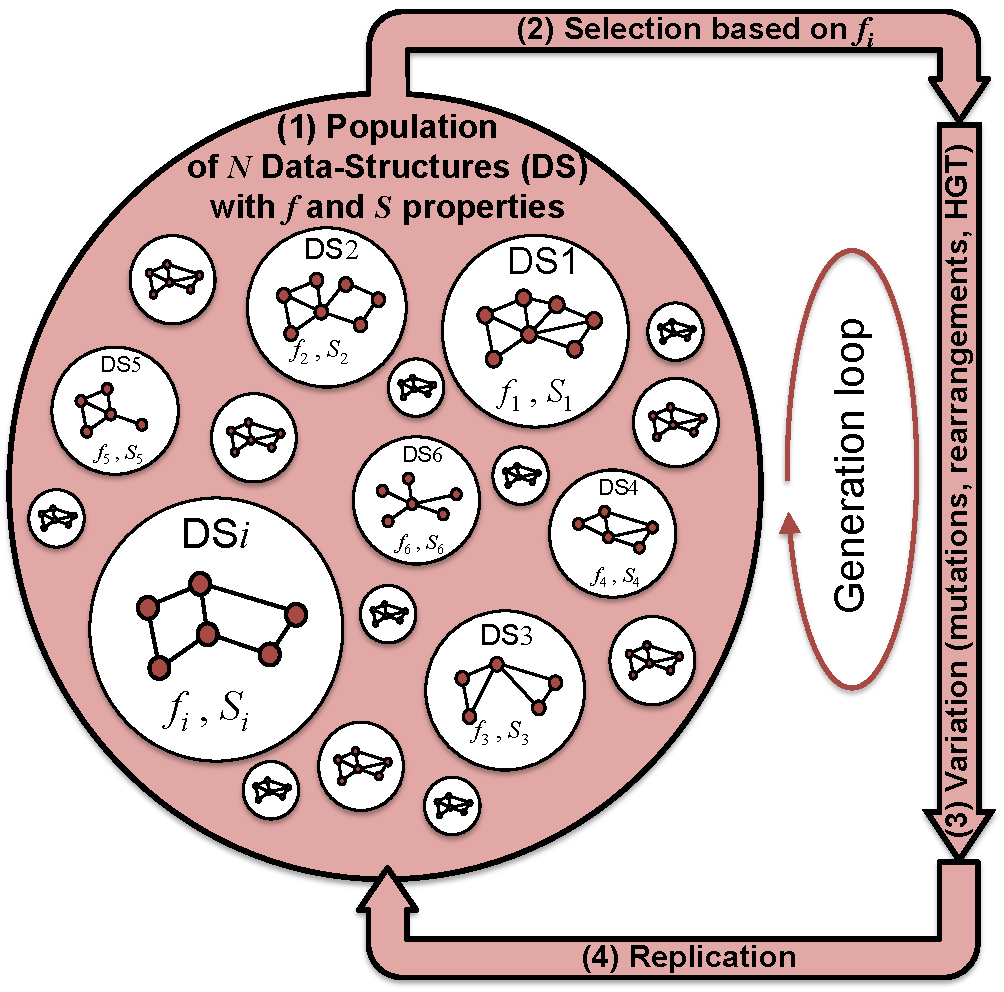
\includegraphics[width=0.75\textwidth]{background/img/evol_sys_bio.pdf}
\caption[Template of an evolutionary systems biology simulation]{Template of an evolutionary systems biology simulation.
In a population of complex systems, each individual $i$ is represented by an inner data structure $DS_i$, from which systemic properties of interest $S_i$ emerge, and that is used to compute a fitness level $f_i$.
The population can then evolve by following an evaluation-selection-variation-replication loop.
Figure reproduced with permission from~\citep{beslon2021}.}
\label{fig:background:evol-sys-bio}
\end{figure}

The core of this approach is represented in Figure~\ref{fig:background:evol-sys-bio}, which describes the evolution of a population of complex systems, or ``digital organisms''~\citep{adami2006}.
Each complex system in the population is represented by the means of a data structure $DS_i$, which represents an instantiation of  underlying system with a particular set of parameter values.
Using this data structure, we can evaluate the systemic properties of interest $S_i$ of this individual, and its fitness value $f_i$.
A new population of complex systems can then be created by selecting reproducers based on fitness, and making their underlying data structure undergo stochastic mutations that can affect both their systemic properties and their fitness.
This cycle can then be repeated for a given number of generations, resulting in an experimental framework called ``\emph{in silico} experimental evolution'', as it adapts the traditional \emph{in vivo} experimental evolution methodology to the computational study of the evolution of arbitrary complex systems.

Both \emph{Aevol} (introduced in Chapter~\ref{chap:aevol}) and \emph{EvoTSC} (introduced in Chapter~\ref{chap:alife}), the \emph{in silico} artificial evolution platforms that I developed and used during my PhD, follow this methodology.
In both platforms, each complex system represents a given individual which is described by its genome; the models diverge in the data structure with which they represent genomes, as \emph{Aevol} is a nucleotide-level model whereas \emph{EvoTSC} is a ``string-of-pearls'' model, in which genomes are represented by a series of genes separated by non-coding sections (see~\cite{hindre2012} for an overview of these formalisms).
The fitness of individuals is obtained in both platforms by evaluating their gene transcription levels, and comparing these transcription levels to an implicit (in \emph{Aevol}) or explicit (in \emph{EvoTSC}) target.
Finally, the systemic properties of individuals differ in each model, according to their choice of underlying data structure: \emph{Aevol} can be used to study properties such as genome size or the proportion of coding bases, whereas \emph{EvoTSC} can be used to study the arrangement of genes on the genome.


\section{Conclusion}

The level of DNA supercoiling is an interesting property of bacterial genomes, standing at the crossroads of many processes: it is finely regulated by the joint action of topoisomerases and nucleoid-associated proteins, but remains sensitive to the external influence of environmental stress, and to the internal influence of gene transcription.
The repeated mutations targeting the regulation of the supercoiling level in the \emph{LTEE} demonstrate the role that supercoiling can play -- through its central position in genome biology -- in the adaptation of bacterial populations to new environments, and make it an ideal example to study the role of epistatic interactions in guiding evolutionary trajectories.
Moreover, as gene transcription itself depends on DNA supercoiling, the resulting interplay between transcription and supercoiling generates a complex web of interactions between neighboring genes in the dense bacterial genomes: the transcription-supercoiling coupling.
While the effect of this coupling has already well been studied at the scale of a few neighboring genes, expanding this analysis to the whole-genome scale seems necessary in order to have a qualitative understanding of the phenotypic consequences of supercoiling mutations, and hence of their possible epistatic interactions.

Finally, an \emph{in silico} experimental evolution approach seems to be the most promising way to tackle the study of the evolutionary role of these mutations, as this methodology enables the combination of a complex model of the transcription-supercoiling coupling -- an integral part of gene regulation by DNA supercoiling -- with an evolutionary model that allows for the emergence of complex epistatic interactions that can influence evolutionary trajectories.

\chapter{Looking for Supercoiling Epistasis in \emph{Aevol}}
\label{chap:aevol}

In this chapter, I present the first main line of work of that I undertook during my Ph.D.
In order to understand the role of epistasis in the prediction of evolution, I focused on the study of the specific case of mutations affecting the DNA supercoiling level in bacteria, which were shown to be repeatable at the phenotypic level, and partially repeatable at the molecular level, in an experimental evolution setting.
In order to replicate these results in the easier to study \emph{in silico} artificial evolution setting offered by the \emph{Aevol} software platform, I implemented a model of supercoiling in \emph{Aevol}, and tried to detect epistatic interactions in the evolutionary trajectories of populations that evolved in the model.

\section{Introduction}
\label{sec:aevol:intro}

In the \emph{Long-Term Evolution Experiment} (LTEE), started by Richard Lenski in 1988~\citep{lenski1991}, 12 populations of \emph{E. coli} cells, originating from the same ancestral strain, were placed to evolve in a new environment, an Erlenmeyer flask containing a glucose-limited medium.
Every day since the beginning of the experiment, which has reached over 75,000 generations of bacteria and is still running, a sample from each population has been propagated into fresh medium, and samples have been cryogenically conserved every 500 generations, resulting in the longest-running evolution experiment in the lab.
The LTEE demonstrated that fitness can keep on increasing for much longer than originally expected in a constant environment~\citep{good2017}.
As sequencing capacity and synthetic biology subsequently developed in the late 1990s and early 2000s, identifying the precise DNA mutations underpinning these increases in fitness became possible.
When sequencing the conserved \emph{E. coli} lineages in the LTEE, beneficial mutations -- mutations that confer on their bearer a higher growth rate than the ancestral strain in the conditions of the experiment -- were in particular found in the \emph{topA} gene and the \emph{fis} gene, in one of the twelve lineages~\citep{crozat2005}.

The genes affected by these mutations are involved in the regulation of DNA supercoiling: Topoisomerase I (encoded by \emph{topA}) directly modifies the supercoiling level by introducing supercoils, and FIS (encoded by \emph{fis}) is a nucleoid-associated protein which helps regulate supercoiling by binding to DNA.
This makes these mutations extremely interesting in two regards.
First, there is no direct phenotypic link between the supercoiling level of the chromosome and the growth rate of the bacteria, and yet these mutations, when inserted into the genetic background of the ancestral strain, still confer a fitness advantage.
Second, mutations affecting supercoiling-regulating genes, especially in \emph{gyrA} and \emph{fis}, were subsequently found in 11 of the 12 replicates of the experiment after 20,000 generations of evolution, a rate that is much higher than for randomly chosen genes~\citep{crozat2010}.
A possible interpretation of this repeated mutational targeting of supercoiling-regulating genes is that, by globally altering the transcriptional landscape of the bacteria (as the level of supercoiling directly affects gene transcription), these mutations enable the exploration of new evolutionary pathways that would have been deleterious in the ancestral strain, and enable the lineages that bear these mutations to evolve faster than the competing strains.
In other words, there could be positive epistatic relationships between these mutations and the subsequent adaptive mutations that they enable through rewiring the fitness landscape of their bearer lineages.

In this chapter, I describe how I leveraged the \emph{Aevol} \emph{in silico} experimental evolution platform in order to test this evolutionary hypothesis in the simpler, more controlled setting of artificial evolution.
\emph{Aevol} is a model that is particularly well-suited to this problem, for several reasons.
First, the genome biology of individuals is modeled very precisely in \emph{Aevol}.
The genome is described at the nucleotide level, and the transcription and translation stages that constitute the core of biological gene expression are accurately represented in the model.
Second, \emph{Aevol} incorporates a rich variety of mutational operators.
It includes both genomic rearrangements such as inversions and translocations or duplications and deletions, and local mutations such as indels and switches.
The richness of the genome-level description of \emph{Aevol} therefore makes it an ideal tool for the study of epistatic relationships.

The chapter starts with a brief overview of the \emph{Aevol} model; then, I present the model of supercoiling and its effect on transcription that I incorporated into the model, and describe the experiment that I performed in order to test the presence of epistasis between supercoiling mutations and other kinds of mutations.

\section{The \emph{Aevol} model}
\label{sec:aevol:model}

\begin{figure}
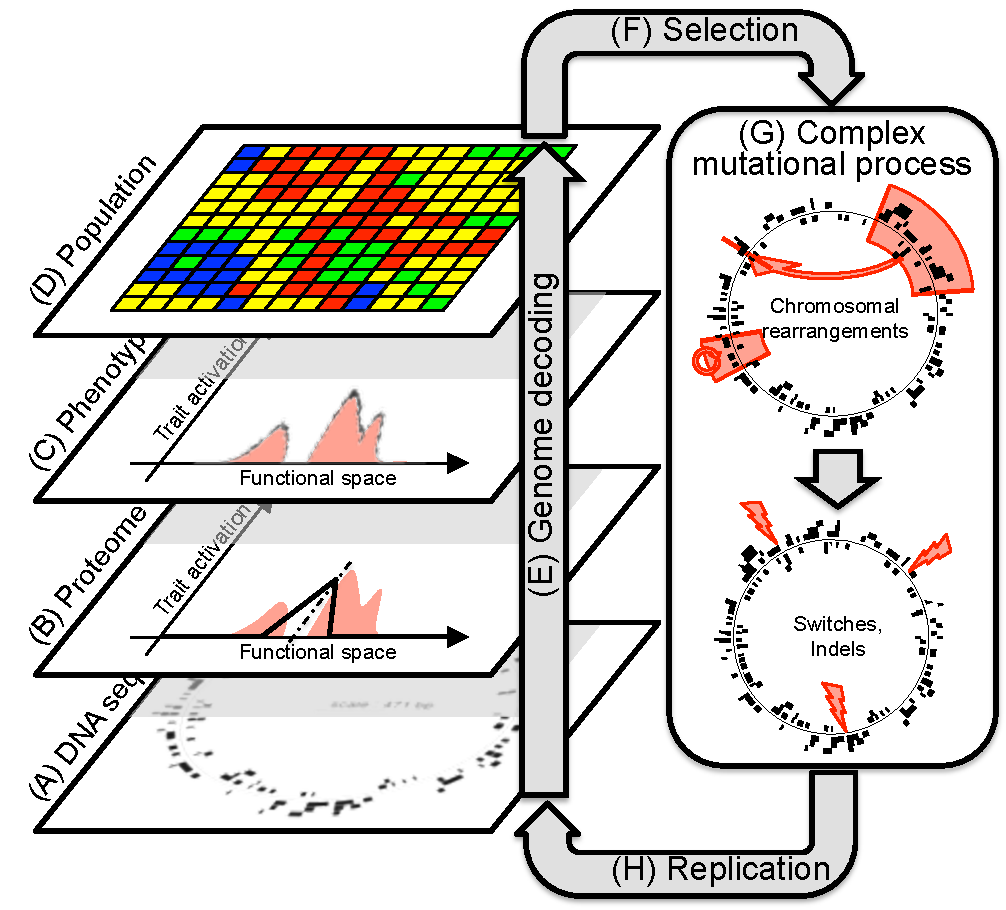
\includegraphics[width=\textwidth]{aevol/images/aevol.pdf}
\caption[Overview of the \emph{Aevol} model]{Broad overview of the \emph{Aevol} model.
In \emph{Aevol}, an evaluation-selection-replication evolutionary loop is applied to a population of individuals defined by their genome, encoded as a circular string of nucleotides (A, central ring), on which RNA sequences and genes are decoded (A, black segments).
The resulting proteins (B, in black) are mapped to an abstract phenotypic space, and summed in order to obtain the phenotype of the individual (C, in black), which is compared to an optimal phenotype (that implicitly represents the environment -- B and C, in pink), in order to compute its fitness.
In the model, the population is laid out on a square grid (D), with one individual per cell.
In order to produce a new generation, the ancestor of the new individual in each cell is chosen at random among the neighboring individuals, proportionally to their fitness (F).
Once this ancestor is chosen, its genome undergoes a series of random mutations, including rearrangements and local mutations (G), in order to obtain the genome of the new individual in the cell at the next generation (H).
}
\label{fig:aevol:model}
\end{figure}

\subsection{Overview}

The \emph{Aevol} platform, developed in the Inria Beagle team~\citep{rutten2019}, is a software suite designed to run artificial evolution experiments on a computer, rather than at the bench.
It was originally created to investigate the influence of classical population genetics parameters such as population size, mutation rate, or selection pressure on genomes themselves, seen as an integral part of the phenotype and not only as the source of genetic information.
In \emph{Aevol}, individuals have a very abstract phenotype, in exchange for a genome that is modeled down to the nucleotide level, and follows the ``central dogma of molecular biology''~\citep{crick1958}, with an accurate representation of RNA transcription and gene translation.
This approach contrasts with other artificial evolution platforms such as \emph{Avida}~\citep{adami1994,ofria2004}, which aim at studying the evolutionary process itself, rather than its impact on biological organisms.
For instance, \emph{Aevol} has been used to study the effect of mutation rate on genome size~\citep{knibbe2005}, or of the selection pressure on the percentage of non-coding bases and number of genes on the genome~\citep{batut2013}.
As an excellent and very thorough description of \emph{Aevol} (in French) can be found in~\cite{liard2020}, the following presentation of the model will be kept short and focused on the aspects relevant to this research.
Figure~\ref{fig:aevol:model} provides a comprehensive overview of the evolutionary algorithm at the core of \emph{Aevol}.

\subsection{The Genotype-Phenotype Map in \emph{Aevol}}

A genome or genotype in \emph{Aevol} consists in a sequence of binary characters ($0$ or $1$), which represents a double-stranded circular sequence of DNA.
The genome sequence explicitly describes the first (forward) strand of DNA, while the second (reverse) strand is obtained by complementing the sequence, replacing $0$ by $1$ and vice-versa.
In order to turn this genotype into a phenotype (Figure~\ref{fig:aevol:model} C), the decoding algorithm starts by looking for sequences that code for RNAs, reading the forward strand left-to-right and the reverse strand right-to-left.
An RNA starts with a promoter sequence, which has to match a consensus sequence with up to $d_{max}$ errors, and ends with a hairpin-like terminator.
Then, each RNA is scanned for genes, which start with a ribosome binding site followed by a 3-nucleotide start codon, which defines the reading frame.
Reading continues until a stop codon is found in the same frame, and the resulting string of codons is then translated into a protein, or discarded if no stop codon is found in frame before the end of the RNA sequence.
An RNA can thus contain zero, one, or several protein-coding genes.

As the genetic alphabet is binary in \emph{Aevol}, there are 8 different 3-nucleotide codons, and 6 codons can therefore be used to encode protein data, in addition to the start and stop codons.
These codons are grouped into three pairs, each respectively encoding the width $w$, height $h$, and mean position $m$ of a triangle kernel function from $[0, 1]$ to $[0, 1]$ (as represented in Figure~\ref{fig:aevol:model} B).
The mean $m$ represents the main function that the protein fulfills in the abstract phenotypic space, the height $h$ the intensity with which it does, and the width $w$ the pleiotropic ability of the protein to fulfill neighboring phenotypic functions.

In order to obtain the final contribution of the protein to the phenotype, the constitutive height $h$ of the gene is weighted by the expression level $e$ of the RNA that carries the gene, which depends on the activity of the promoter of that RNA.
In the model, the promoter activity decreases linearly with the difference $d$ between its sequence and the consensus sequence, and vanishes when $d > d_{max}$.
The expression level of the RNA is then given by the following equation: $e = 1 - \frac{d}{1+d_{max}}$.
Finally, in order to compute the complete phenotype of the individual from the set of its proteins, the kernel functions representing each gene are summed, resulting in a piecewise-linear phenotype function.
As the maximum degree to which each phenotypic function can be fulfilled is bounded by 1, the phenotype function is finally capped using Łukasiewicz operators in order to keep within this limit.

\subsection{Fitness}

Once the phenotype of an individual has been decoded from its genome, we can compute its fitness.
As the environment is indirectly specified by an optimal phenotype, we first compute a phenotypic gap as the integral of the absolute value of the difference between the phenotype of the individual and the optimal phenotype, taken over the range of phenotypic values (the $L^1$ distance between the functions).
Then, we compute the fitness as the inverse exponential of the phenotypic gap, multiplied by a selection coefficient: the higher the coefficient, the larger the difference in fitness between individuals with the same difference in gap.

\subsection{Mutational Operators}

Once the ancestor of a new individual has been chosen, a set of random mutations are applied to its genome to obtain the new genome.
These mutations are split into two classes, depending on the proportion of the genome that they can affect: genomic rearrangements, and local mutations.

Genomic rearrangements can affect up to the whole genome, and comprise four kinds of structural changes: duplications, deletions, inversions, and translocations.
In each of these rearrangements, the two endpoints of the affected segment are first drawn randomly on the genome.
In a large duplication, an additional insertion point is randomly selected on the genome, and the genetic content located between the endpoints is copied at the insertion point.
In a large deletion, the genetic content that was present between the endpoints is simply discarded.
In an inversion, the segment is reinserted left-to-right between the endpoints, reversing the orientation of every gene located on the inversion.
Finally, in a translocation, the genetic content is removed, turned into a circular plasmid, cut at a random point in the plasmid, and reinserted at another insertion point in the genome.

Local mutations, on the contrary, comprise small insertions, small deletions (collectively known as indels), and switches.
In a small insertion or deletion, up to 6 contiguous bases are either inserted (choosing each base at random) or deleted at a random point in the genome.
In a switch, the value of a random nucleotide is switched, from 1 to 0 or vice-versa.


\section{Modeling DNA Supercoiling in \emph{Aevol}}
\label{sec:aevol:aevol_sc}

In order to model the effect of supercoiling on gene transcription in \emph{Aevol}, I chose to start with very simple approximations,
concerning the level of supercoiling itself and its effect on transcription, as the \emph{Aevol} model is already quite complex on its own.

\begin{figure}
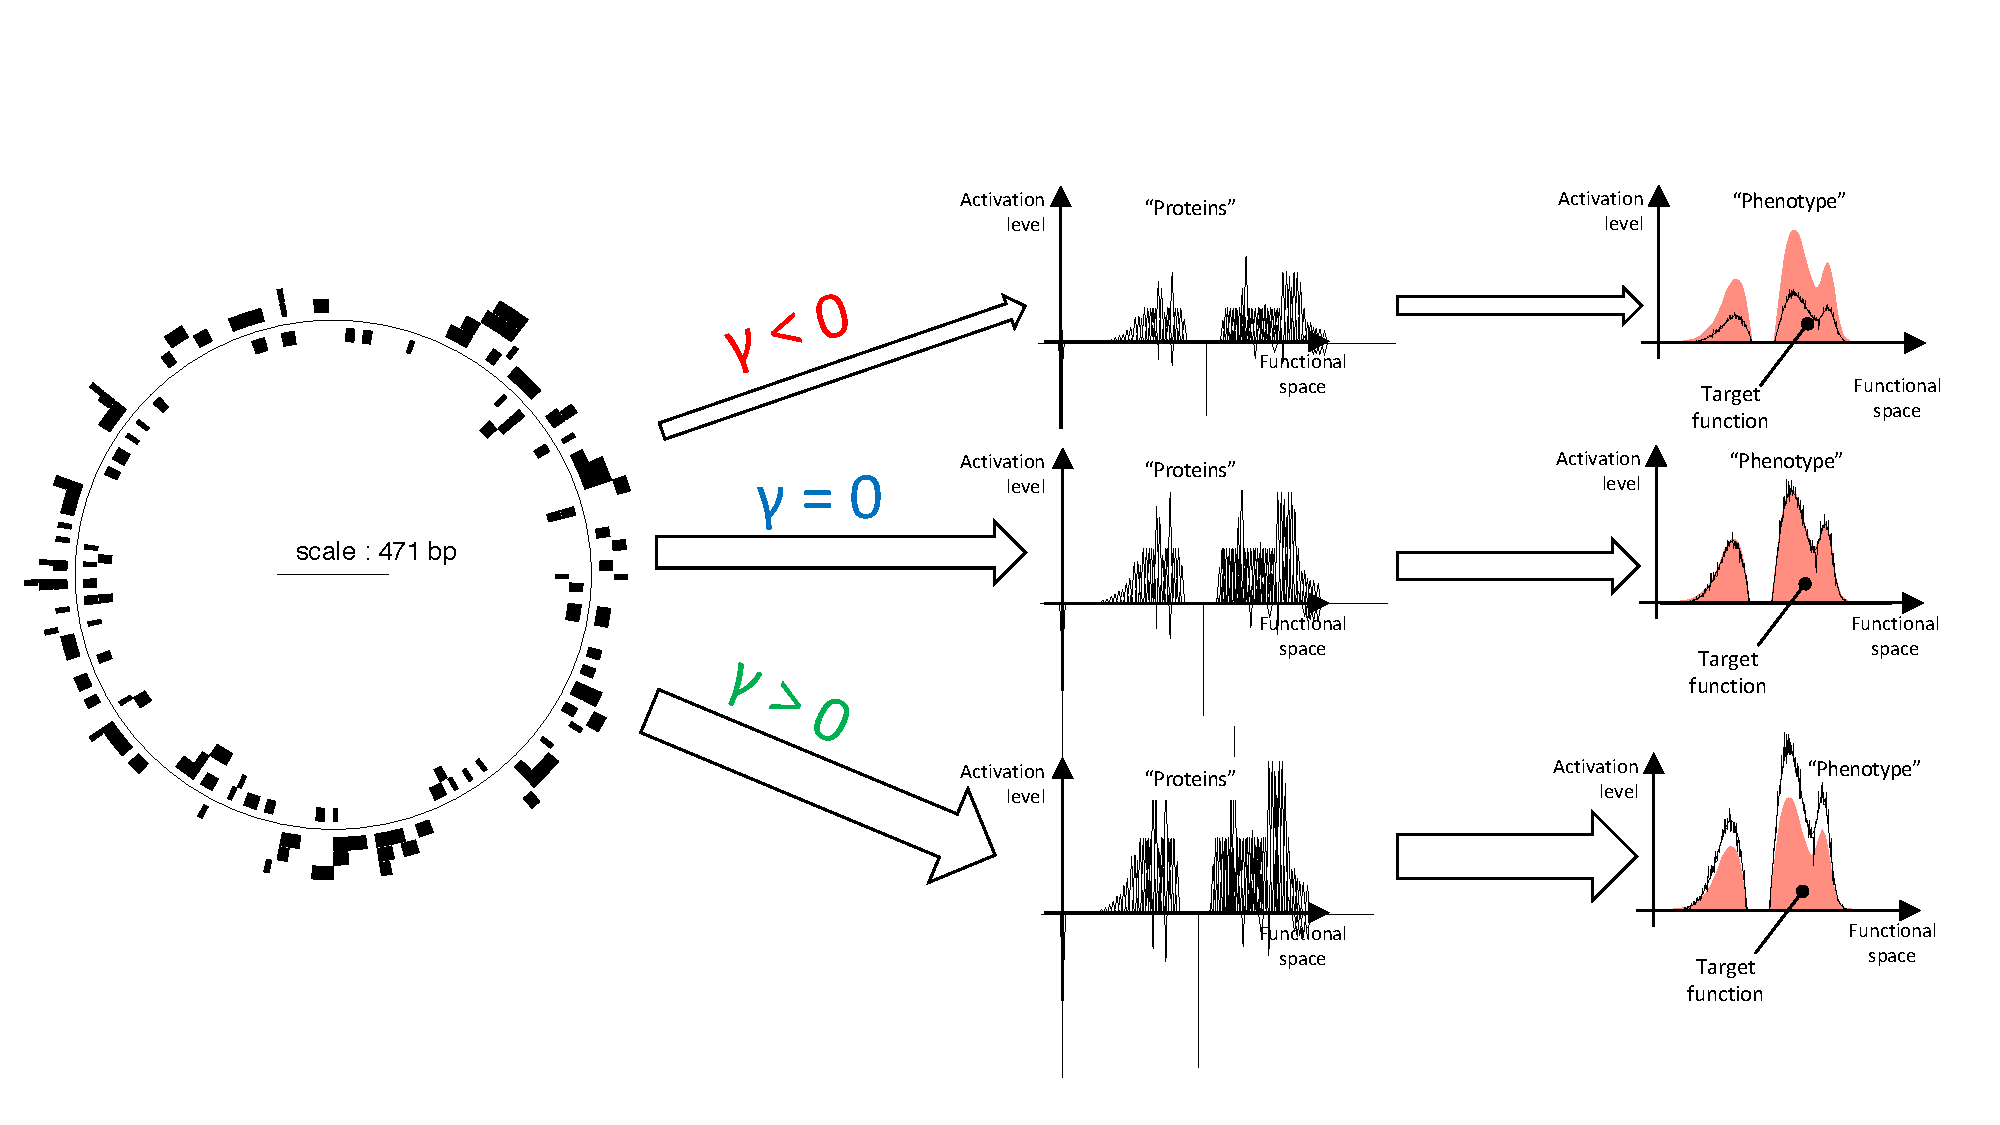
\includegraphics[width=\textwidth]{aevol/images/supercoiling_aevol.pdf}
\caption[Effect of supercoiling on the phenotype of an individual in \emph{Aevol}]{Effect of supercoiling on the phenotype of an \emph{Aevol} individual.
Left: genome (central ring) and genes (black rectangles) of the individual.
Middle: kernel function encoded by every gene in the phenotypic space, affected by an excess of positive supercoiling (top), no extra supercoiling (middle), or an excess of negative supercoiling (bottom).
Right: phenotype of the individual in each situation, compared to the optimal phenotype (in pink).}
\label{fig:aevol:sc_phenotype}
\end{figure}

\subsection{Level of DNA Supercoiling}
First, I consider the supercoiling level as constant along the genome and over time, which can be interpreted as taking the spatial and temporal average of the (actually dynamic) supercoiling level.
To implement this model inside \emph{Aevol}, I changed the genotype of individuals by adding, alongside the string-of-nucleotides genome, a single parameter $\gamma$ which represents the relative variation in the supercoiling level $\sigma$ of this individual compared to a reference supercoiling level $\sigma_0$: $\gamma = \frac{\sigma-\sigma_0}{\sigma_0}$.

\subsection{Gene Expression}
To keep the model as simple as possible, I also chose to model the effect of supercoiling on transcription as having the same linear effect on the transcription rate of every RNA on the genome.
I therefore updated the computation of the gene expression $e$ to take supercoiling into account, in addition to promoter activity:

\begin{equation}
e = (1 - \frac{d}{1+d_{max}}) \cdot (1 + \gamma)
\label{eq:aevol:sc}
\end{equation}

The effect of supercoiling on the phenotype of an example (pre-evolved) individual in the model is presented in Figure~\ref{fig:aevol:sc_phenotype}.
When $\gamma < 0$ (top row) -- when there is an excess of positive supercoiling compared to the baseline -- the expression of every gene is decreased.
When $\gamma$ is equal to 0 (middle row) -- when the supercoiling level is equal to the baseline -- there is no change to gene expression levels, which replicates the behavior of the original \emph{Aevol} model.
Finally, when $\gamma > 0$ (bottom row) -- when there is more negative supercoiling than in the baseline -- the expression of every gene is increased.

\subsection{Mutational Operator}
\label{sec:aevol:mut-sc}

In biological organisms, the supercoiling level is not only a direct property of the DNA molecule, but is also controlled by topoisomerases and nucleoid-associated proteins that are not modeled in \emph{Aevol} (as the phenotypic space is completely abstract), and changes in the supercoiling level come from mutations affecting the genes that encode these proteins, such as \emph{gyrA} or \emph{fis}~\citep{crozat2005}.
In order to model mutations in the supercoiling level in \emph{Aevol}, I chose a continuous model, in which a small variation in $\gamma$ indirectly reflects the effect of a mutation in one of the supercoiling-controlling genes.

When an individual reproduces, we first use a Bernoulli trial, with a probability $p$ that represents the probability that a supercoiling-protein gene undergoes a non-synonymous mutation, to decide whether to change the supercoiling level.
Then, if the supercoiling level should change, we draw a variation in relative supercoiling $\Delta\gamma$ according to a normal distribution $\mathcal{N}(0, s^2)$, and finally set the relative supercoiling level $\gamma'$ of the offspring to $\gamma' = \gamma + \Delta\gamma$.
The parameters of these laws are parameters of the simulation, and their values are given in Table~\ref{tab:aevol:param_values}.
Throughout this chapter, I will for the sake of clarity refer to the usual DNA-affecting mutations presented in~\ref{sec:aevol:model} as \emph{genomic mutations}, and to the mutations in the supercoiling level presented here as \emph{supercoiling mutations}.


\section{Results}
\label{sec:aevol:results}

As presented in the introduction of this chapter, the goal of implementing a supercoiling model in \emph{Aevol} was twofold.
The first aim was to see to which extent adding a new dimension to the phenotypic space, and a new mutational operator to explore this new dimension, would allow populations to evolve faster than allowed by the original model, thanks to the wide jumps in the phenotypic landscape that are made possible by the supercoiling mutations.
The second aim was to disentangle the possible epistatic effects between supercoiling mutations and genomic mutations in \emph{Aevol}.
In this section, I first present the experimental setup that I used in order to answer these questions.
Then, I show that adding regulation by supercoiling did not measurably increase the rate of adaptation of populations compared to the control, and that supercoiling indeed follows a very constrained evolutionary trajectory in these experiments.
Finally, I conclude that I could not find any observable epistasis between supercoiling and other mutations, when using the supercoiling model presented in Section~\ref{sec:aevol:model}.

\subsection{Experimental Setup}

In order to tackle these questions, I ran two sets of simulations: the experimental runs using the supercoiling model, and the control runs using the vanilla version of \emph{Aevol}.
Each set of runs comprises 5 replicate populations, which were evolved for 1,000,000 generations, each starting from a clonal population.
Each of the initial individuals was obtained by randomly drawing 5,000 bp-long genomes, until a genome with a non-zero fitness (i.e., at least one protein-coding gene partially matching the phenotypic target) was found.
The simulations were run on a 24-core Intel(R) Xeon(R) CPU E5-2620 v3 @ 2.40GHz server with 128 GB of RAM, and lasted approximately a week for each set of replicates.
The limited number of replicates for each set of simulations was chosen to balance their energy expenditure with the preliminary character of the work, which alleviates the need for statistical strength in the resulting data.
All the data from this experiment is available online on the \href{https://doi.org/10.5281/zenodo.7307545}{Zenodo} platform.

\subsection{Studying Lineages}

The data that is presented in the rest of this section was obtained by reconstructing the lineage, starting from the initial generation, of a random individual at the last generation of each replicate.
Studying a given lineage, rather than the best individual at every generation (which need not sire one another), allows us to reconstruct the precise set of mutations that happened throughout the evolutionary history of this lineage, and therefore gives us information about the possible causal link between these mutations, and hence about their possible epistatic relationships.

As a theoretical haploid Wright-Fisher population with $N$ individuals coalesces on average in $2N$ generations without mutation or selection~\citep{felsenstein2019}, we chose to analyze the data from generation 0 to 990,000 of every replicate (excluding the last 10,000 generations), ensuring that the last individual in each lineage is indeed ancestral to the whole population of the last generation of that replicate.

\begin{table}
\begin{center}
\begin{tabular}{ l r r }
\toprule
\textbf{Parameter} & \textbf{Symbol} & \textbf{Value}\\
\midrule
Population size & N & 1,024 (32x32 grid) \\
Initial genome size & $g_0$ & 5,000 bp \\
Local mutation rate & $\mu_{loc}$ & $10^{-7}$ bp$^{-1}$.gen$^{-1}$ \\
Rearrangement rate & $\mu_{rear}$ &$10^{-6}$ bp$^{-1}$.gen$^{-1}$ \\
\midrule
Initial supercoiling level & $\gamma_0$ & 0 \\
Supercoiling mutation probability & $p$ & $10^{-1}$ \\
Supercoiling mutation variance & $s^2$ & $10^{-2}$ \\
\midrule
Generations & T & 1,000,000 \\
Number of replicates & $n$ & 5\\
\bottomrule
\end{tabular}
\end{center}
\caption[Table of parameter values for the \emph{Aevol} runs]{Table of parameter values used in the \emph{Aevol} evolutionary runs.
The top part describes parameters common to the experimental and control set of rules, the middle part the supercoiling-related parameters introduced in the supercoiling model, and the bottom part simulation-specific parameters.}
\label{tab:aevol:param_values}
\end{table}


\subsection{Evolution of the Fitness Level}

\begin{figure}
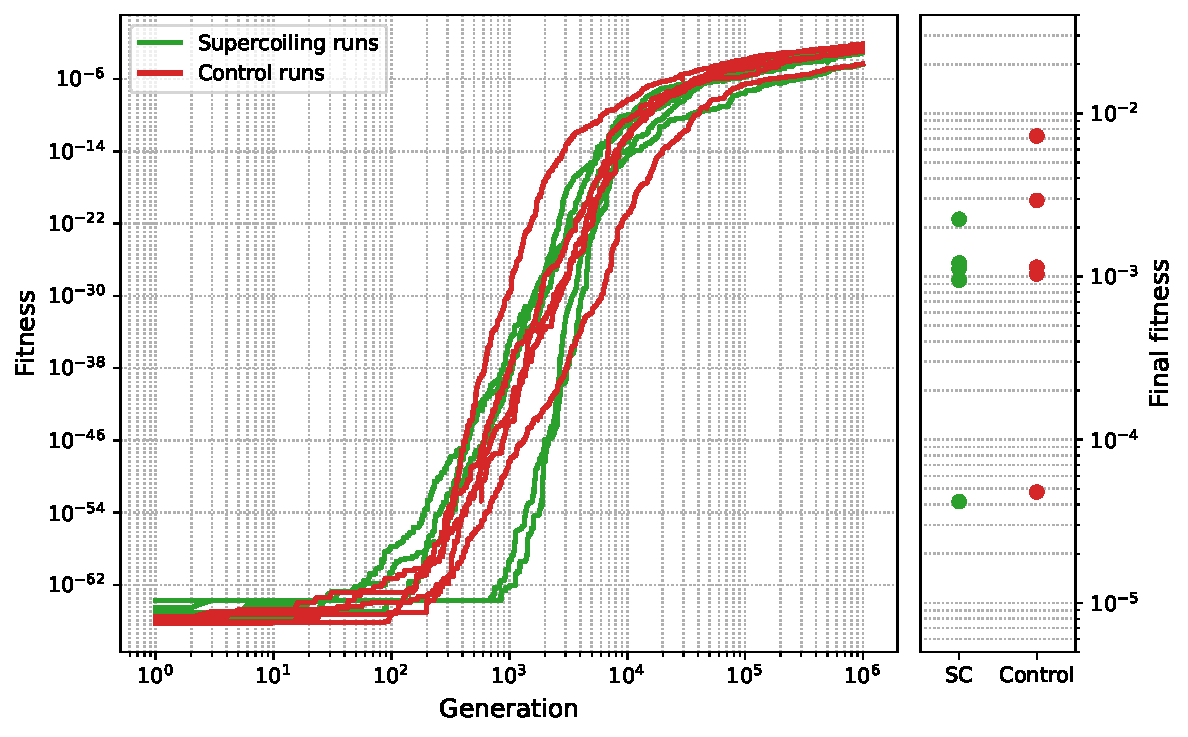
\includegraphics[width=\textwidth]{aevol/images/fitness_all.pdf}
\caption[Evolution of the fitness of the control and experimental runs in \emph{Aevol}]{Left: Evolution of the fitness at every generation throughout the lineage of the final population of each replicate of the experimental (green) and control (red) runs.
Both axes follow logarithmic scales.
Right: Fitness of the lineage individual at the 990,000th generation of each run, separated between supercoiling (green) and control (red) runs.}
\label{fig:aevol:fitness}
\end{figure}

Figure~\ref{fig:aevol:fitness} presents, on the left-hand side, the fitness of the individual at every generation of the lineage of the final population, or lineage individual, in each replicate.
In each case, fitness follows a broadly sigmoid shape (noting that both axes are logarithmic): the fitness of each run quickly increases from generation 100 up to generation 100,000, then slows down for the remaining 900,000 generations, but never completely ceases to progress, mirroring in \emph{Aevol} the open-ended evolution observed in the LTEE.
The right-hand side of Figure~\ref{fig:aevol:fitness} shows the fitness of the lineage individual at the 990,000th generation of each run.

With the limited number of replicates of each run, there is no discernible difference in fitness between the two experimental conditions, with and without mutations in the supercoiling level.
Adding the new phenotypic dimension of the supercoiling level, and the associated supercoiling mutational operator, therefore does not seem to play an important role in the rate of evolution of the populations modeled in \emph{Aevol}.

\subsection{Evolution of the Supercoiling Level}

\begin{figure}
\centering
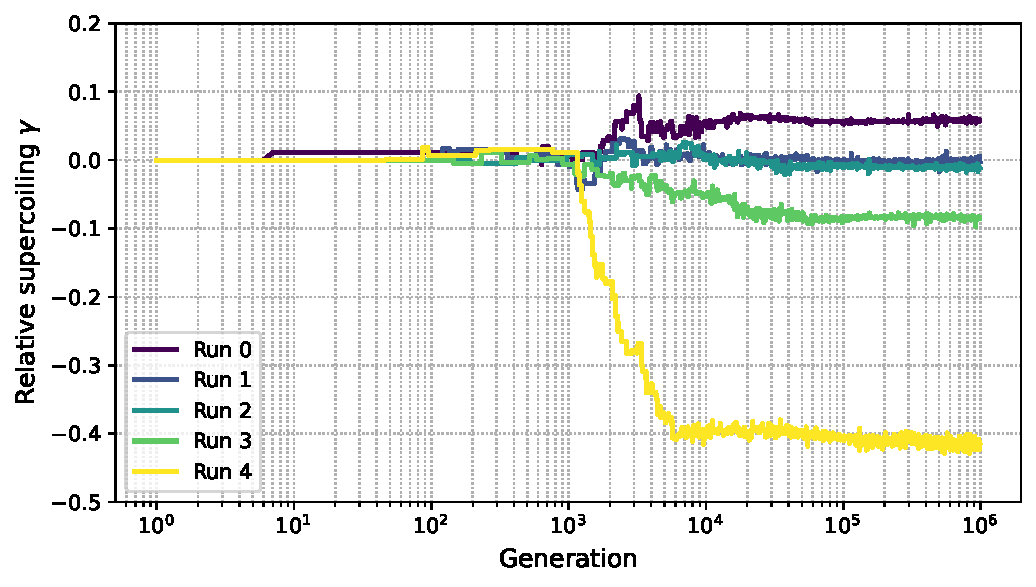
\includegraphics[width=0.9\textwidth]{aevol/images/supercoiling_all.pdf}
\caption[Evolution of the supercoiling level of the experimental runs in \emph{Aevol}]{Evolution of the relative level of supercoiling at every generation of the lineage of each of the experimental runs.}
\label{fig:aevol:sc}
\end{figure}

Figure~\ref{fig:aevol:sc} shows the evolution of the supercoiling level throughout the lineage in each of the 5 replicates.
In every run, the supercoiling level evolves only at the very beginning of the run, stabilizing in a few tens of thousands of generations, and remains essentially constant afterwards.
This is in strong contrast to the fitness of the runs (presented in Figure~\ref{fig:aevol:sc}), which keeps increasing until the end of the runs.

It therefore seems that the supercoiling level might play a role in the early evolution of the runs, but not in their long-term fitness improvement.
This result is in a sense slightly disappointing but was not entirely unexpected.
Indeed, in the early evolution of individuals in \emph{Aevol}, the phenotypic target is only very imperfectly approached by the proteins expressed by the individual.
At that stage, mutations in the supercoiling level, which affect the expression level of every protein equally, could indeed have a positive effect by bringing the whole phenotype closer to the optimum, in a very broad stroke.
Indeed, as individuals in \emph{Aevol} evolve from an ancestor with a single good gene, phenotypic functions are often under-performed by individuals at the early stages of evolution in the model, as the width and height of the kernel functions of their genes can be small, and as the expression level of their RNAs can be quite low if their promoters contain too many errors.
The different supercoiling values towards which each of the replicates tends to converge in Figure~\ref{fig:aevol:sc} could therefore be interpreted as a founding effect coming from the genome of the original individual in that run, which could be confirmed by a more detailed analysis of the series of mutations that happened in each lineage.

However, as evolution progresses, and as the optimal phenotype is more and more closely matched by the individual, changing the whole expression profile at once becomes less and less susceptible to be favorable.
This case is represented in Figure~\ref{fig:aevol:sc_phenotype}: any change in supercoiling, be it positive or negative, will decrease the fitness of the individual, and supercoiling mutations are therefore less and less susceptible to be picked up in the lineage.

These results tend to show that the model in which supercoiling has a global, linear effect on gene expression levels is too simplistic in order to produce phenotypic effects that are variable enough to have a chance to be picked up by selection; and therefore that this model is insufficient to study the interplay between supercoiling mutations and genomic mutations in \emph{Aevol}.

\subsection{Looking for Epistasis}

\paragraph{Waiting Intervals Before and After Mutations}
In order to detect signs of positive or negative epistasis between the different kinds of mutations, I used the following approach, which considers the waiting intervals before and after mutations happen: if, for a given mutation type, the average interval until a new favorable mutation fixes in the lineage after a mutation of that type is smaller than the average interval since the last favorable mutation before that mutation, this could be interpreted as a sign that the mutation has increased the probability of a favorable mutation happening; in other terms, as a broadening of the evolutionary paths available to the genome, or a sign of positive epistasis between that kind of mutation and other kinds of mutations.
On the contrary, if it takes longer for a new favorable mutation to fix in the lineage after that mutation, it would be a sign that the evolutionary paths have been constrained by the inversion: a sign of negative epistasis.

The data obtained following this approach is presented in Figure~\ref{fig:aevol:epistasis}.
For each mutation type, it shows the average number of mutations of that type that fixed in the lineage of each replicate, as well as the average time after which a mutation of that types fixes after a non-neutral mutation (left), and before a non-neutral mutation fixes after a mutation of that type (right), in the control runs (top) and in the experimental runs (bottom).

\paragraph{Epistasis of Duplications and Deletions}
In the control, a faint pattern seems to be discernible for large-scale inversions and deletions: the average time to a new mutation after a deletion is slightly higher than the time before a deletion, hinting that deletions could present a negative epistasis with other mutations.
Conversely, the time to a new mutation after a duplication is slightly lower than the time before the mutation, hinting that duplications could on the contrary present positive epistasis with other mutations.
Local mutations, as well as rearrangements and inversions, do however not seem to swing one way or the other.

In the experimental runs, no such pattern is visible at first sight, including for the supercoiling mutations, and the global average waiting intervals are smaller than in the control, which is consistent with the introduction of a new mutation type.
There therefore seems to be no sign of epistasis between supercoiling mutations and genomic mutations, when following the approach explained above.

\begin{figure}
\centering
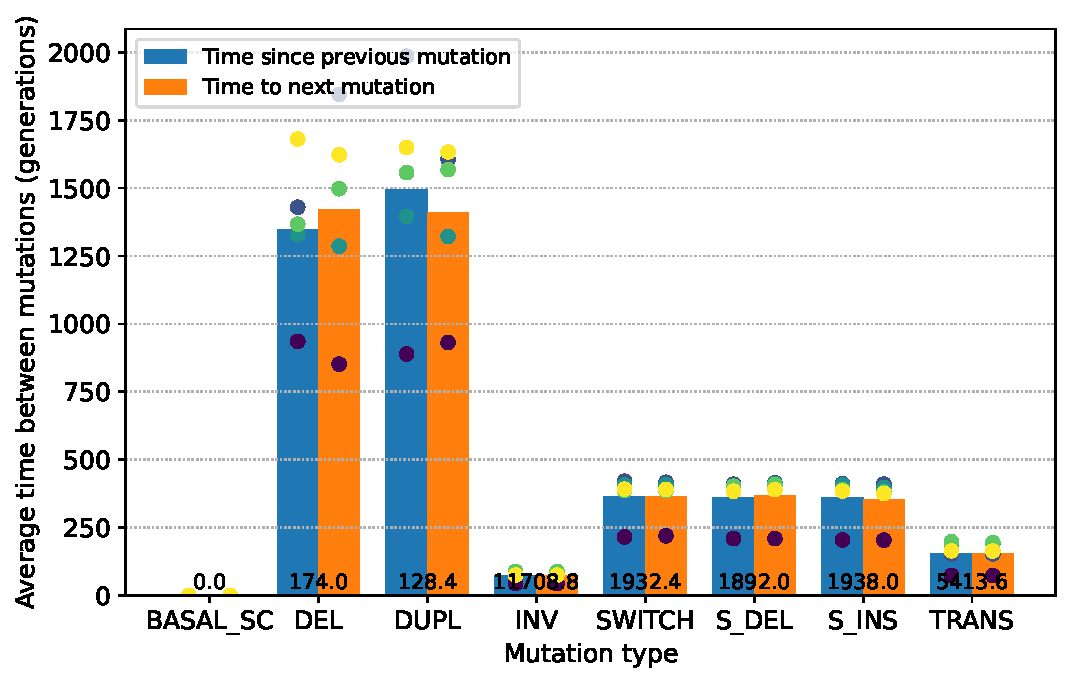
\includegraphics[width=0.9\textwidth]{aevol/images/epistasis_control.pdf}
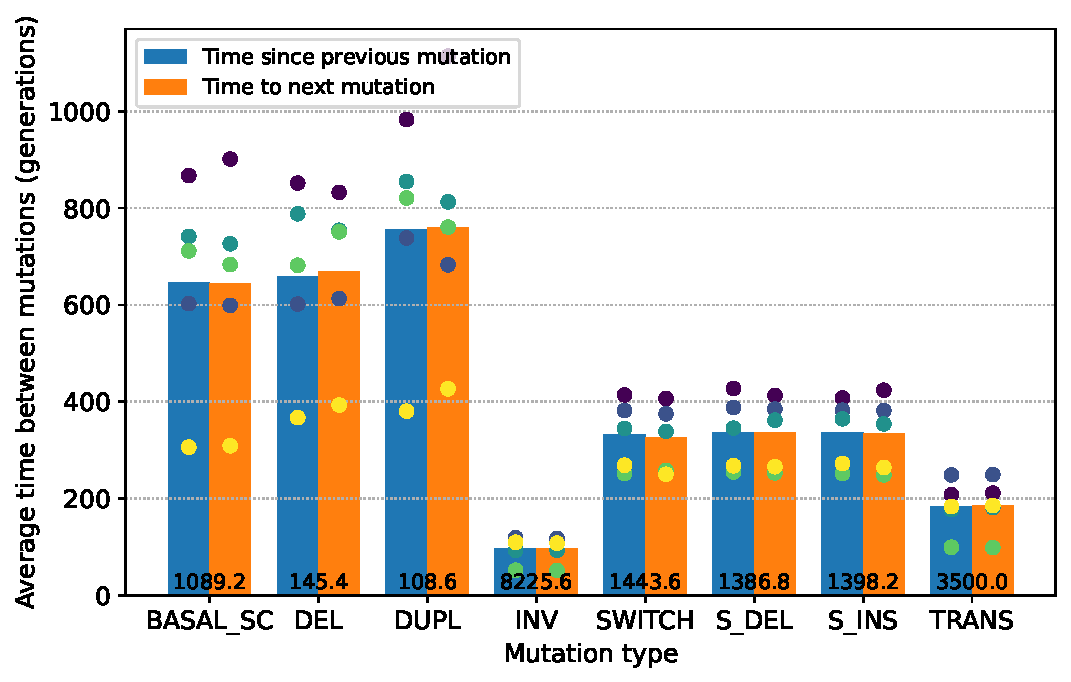
\includegraphics[width=0.9\textwidth]{aevol/images/epistasis_sc.pdf}
\caption[Measuring epistasis with the average times before and after mutations]{Average time before and after a mutation of each kind, in the control runs (top) and the experimental runs (bottom).
For each kind of mutation, the times presented show the wait time until a neutral mutation of that kind after a non-neutral mutation of any kind, and the time until the next non-neutral mutation of any kind after a mutation of that kind.
The bars show the average over the five replicates, and the colored dots show the value for every replicate.
The average number of neutral mutations of each type is displayed at the bottom of the corresponding bar.}
\label{fig:aevol:epistasis}
\end{figure}

\paragraph{Role of the Genome Size}
A hypothesis that could explain the pattern visible in the control runs for large deletions and duplications is that the difference in waiting intervals -- positive or negative epistasis -- is simply due to the change in the genome size caused by these mutations.
All mutation rates in the model are indeed proportional to the genome size, and the expected number of mutations at each generation therefore increases and decreases with the genome size (assuming that there is no fitness effect or selection).
However, in the experimental runs, the probability of a supercoiling mutation does importantly not depend on the genome size.
A hypothesis to explain the disappearance of the signal (possibly) there in the control for duplications and deletions could therefore be that supercoiling mutations tick according to their own clock, which depends on their parameters $p$ and $s^2$, but not on the state of the genome itself.
For example, if a certain beneficial indel is allowed to happen because of a duplication and indeed happens sometime after that duplication in the lineage, but a supercoiling mutation has happened between the duplication and the indel, then the signal from this particular epistatic relationship will have been hidden by that supercoiling mutation.

\section{Conclusion}
\label{sec:aevol:ccl}

The goal of this initial work was to study how supercoiling mutations affect the fitness landscape of individuals in \emph{Aevol}, that is the possible epistatic interactions between supercoiling mutations and other kinds of mutations.
In order to tackle this question, I implemented a model of the effect of the supercoiling level on gene expression, as well as a model of mutations in the supercoiling level, in \emph{Aevol}.
Using this version of the model, I ran evolutionary experiments, in which I compared the evolution of populations with supercoiling with control populations by analyzing the fitness, supercoiling level, and mutations fixed in the lineage of individuals that leads to the final population of every replicate.

With the limited data that was available, I could not find a difference in the evolution rates of each set of experiments, and deduced that supercoiling does not seem to play an important evolutionary role in this model; this result was substantiated by the fact that the supercoiling level converges very quickly to a fixed level in the evolutionary history of each population.
I then tried to detect signals of positive or negative epistasis between the different kinds of mutations, by looking at the waiting intervals between each kind of mutation.
While this approach did not lead to meaningful results in the experimental runs, it did hint at a possible epistatic link between duplications or deletions and the other mutation kinds, due to their effect on genome size, in the control runs, which seems promising for further investigation.

\paragraph{}
The verdict of these preliminary experiments was that the model of supercoiling that I implemented in \emph{Aevol}, in which supercoiling is kept constant along the genome and affects the expression level of all genes equally, was probably too simplistic to obtain meaningful results.
Rather than pursuing this avenue of research further by implementing a more precise model in \emph{Aevol}, I chose instead to go in a different direction.
In order to decouple the complexity of the \emph{Aevol} model from the study of the evolutionary role of supercoiling, I decided to simplify the individual model, genotype-phenotype map, and mutational operators as much as possible, in order to model the effect of supercoiling on gene expression more precisely while keeping the overall complexity of the model in check.
The results of this renewed approach are presented in the following chapters.
\chapter{Evolution of Environmental Sensing through DNA Supercoiling}
\chaptermark{Evolution of Environmental Sensing through DNA SC}
\label{chap:alife}

This chapter presents the proof-of-concept version of the \emph{EvoTSC} model, and the first results that I obtained with that version of the model: I show that the evolution of differentiated expression levels in different environments is possible when gene expression is only regulated by the transcription-supercoiling coupling.
The text of the chapter is an edited version of an article published in the \emph{Artificial Life} journal~\citep{grohens2022a}.

\paragraph{}
Both the importance of gene regulation via supercoiling and the detailed mechanisms of the transcription"=supercoiling coupling, at the local scale, have already been studied extensively in the literature (see Section~\ref{sec:background:sc}).
However, a thorough analysis of the effect of the transcription-supercoiling coupling on gene expression at the whole-genome scale -- and of its possible evolutionary use by natural selection -- remains lacking, in particular in the dense prokaryotic genomes, in which large groups of genes are likely to interact through this coupling.
In this work, we describe a new model which incorporates a high-level model of global supercoiling regulation and of the transcription"=supercoiling coupling within an \emph{in silico} experimental evolution setting.
Using this model, we first investigate the non-linear variation in gene transcription levels at the whole-genome scale in response to variations in the global supercoiling level.
Then, we study the evolutionary trajectory of gene activation patterns in individuals subjected to different environments.

We show that in our model, a genome-scale gene interaction network emerges from local supercoiling-mediated interactions, and creates a reaction norm in response to the change of a single parameter, the global supercoiling level, caused by different environments.
Moreover, we demonstrate that, using genomic inversions as the only mutation operator, and therefore only changing the relative positions and orientations of genes on the genome, evolution can select genomes displaying qualitatively different phenotypes in different environments characterized by different global supercoiling conditions.

%This article is an extended version of~\cite{grohens2021}.

\section{A Genome-Wide Model of the Transcription-Supercoiling Coupling}
\label{sec:alife:indiv_model}

\begin{figure}[H]
\centering
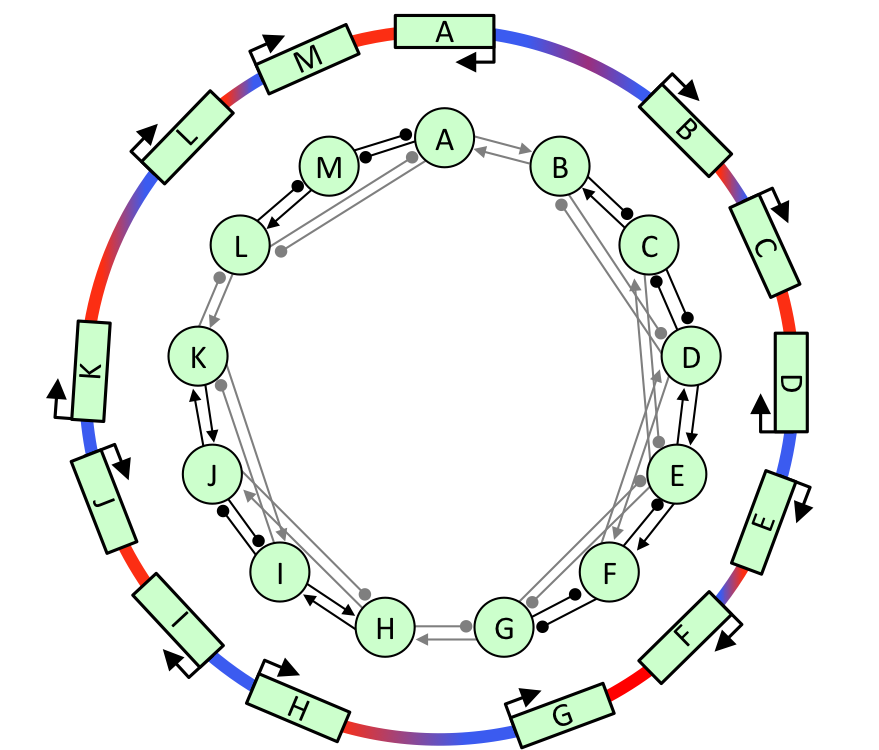
\includegraphics[width=0.75\textwidth]{alife/img/reseau.png}
\caption[Hand-drawn genome and local interactions resulting from the TSC]{Genes along an example genome and local variations in supercoiling (outer ring), and the associated gene interaction network (inner ring).
The outer ring color shows locally high ($\sigma > \sigma_0$, red) or low ($\sigma < \sigma_0$, blue) supercoiling levels due to gene transcription.
In the inner ring, closer genes interact more strongly (black arrows) than genes that are farther apart (gray arrows), either positively or negatively depending on their relative orientations.}
\label{fig:alife:network}
\end{figure}

%In this paper, we present a model which aims at studying the genome-wide effect of the transcription-supercoiling coupling in bacteria, expanding upon previous work which only considered local interactions.
%In gene-dense genomes such as prokaryotic ones, transcription-supercoiling coupling between nearby genes is likely to give rise to a genome-wide transcriptional network, the topology of which depends on relative gene distances and orientations.

Our model consists in an individual-based simulation, written in Python.
Its source code is available at \url{https://gitlab.inria.fr/tgrohens/evotsc/-/tree/alife-journal}.
It is also preserved for \href{https://archive.softwareheritage.org/swh:1:rev:6fc36abc1661c295782886647c37ef05ffb9d357}{long-term archival} using the Software Heritage online archive~\citep{dicosmo2020}.
An individual in the model is represented by a circular genome (representative of most bacterial genomes), comprising a fixed number of genes, separated by non-coding intergenic regions.
Each gene is described by the following characteristics: its locus on the genome, its orientation, and its basal transcription (or expression) level.
As we are mainly interested in the interplay between supercoiling and transcription, we voluntarily do not make the difference between gene expression levels, understood as mRNA or protein concentrations, and transcription levels, the immediate rate of mRNA
production.
Indeed, assuming a separation of timescales between the fast equilibrium of the transcription-supercoiling coupling, and the slow degradation of mRNAs, the concentration of a given mRNA is directly proportional to the transcription rate of its source gene.

Figure~\ref{fig:alife:network} illustrates the role played by the transcription-supercoiling coupling in an example genome.
It includes the local supercoiling variations due to gene transcription, and the resulting gene interaction network, with each gene possibly activating or inhibiting its neighbors, depending on their relative orientations.
Importantly to our approach, here genes do not interact only with their closest neighbors, but also with more distant genes, as is likely to be the case in the gene-rich bacterial genomes: \emph{E. coli} gene promoters are around one thousand base pairs apart~\citep{peter2004}, and the transcription-generated supercoiling propagates around a few thousand base pairs on each side of the transcription site~\citep{postow2004}.


\subsection{Mathematical Description of the Model}

We model the transcription-supercoiling coupling between an individual's genes as a system of equations, which relate the supercoiling level at the locus of each gene $\sigma_i$ (for $i$ ranging from $1$ to $n$, the number of genes of the individual), and the expression level of every gene $e_i$.
The parameters of the system are described by the genome of the individual, as will be detailed below.

In our model, the supercoiling at a given locus on the genome depends on three factors: the individual's basal supercoiling level $\sigma_{basal}$, the variation in supercoiling due to environmental conditions $\sigma_{env}$, and the variation in supercoiling due to the transcription of the neighboring genes.
We compute this local variation in supercoiling at the locus of each gene with the help of a gene interaction matrix, whose coefficient at position $(i, j)$ describes the influence of gene $j$ on gene $i$.
The coefficients are given by the following equation:

\begin{equation}
\frac{\partial\sigma_{i}}{\partial e_j} = \eta\cdot c \cdot\max(1-\frac{d(i, j)}{d_{max}}, 0)
\label{eq:dsde}
\end{equation}
%This interaction level abstracts the influence of local supercoiling into a single value, which reflects the positive or negative influence of each gene on the transcription level of the other genes in the genome.

More precisely, the interaction level between two genes depends on the relative orientation of the genes, as the transcription of a gene increases supercoiling at the locus of downstream genes and decreases supercoiling at the locus of upstream genes (remember that an increase in supercoiling means a decrease in transcription).
Therefore, we choose $\eta = 1$ if gene $i$ is downstream of gene $j$ and $\eta = -1$ otherwise (if $i=j$, $\eta = 0$ as a gene does not interact with itself).
The interaction level also depends on gene distance, as genes that are further apart on the genome interact less strongly, so the strength of the interaction linearly decreases with the intergenic distance $d(i, j)$, and reaches 0 when $d(i, j) = d_{max}$, the maximum distance above which the interaction vanishes.
Finally, an interaction coefficient $c$ is applied to adjust the strength of the coupling.

Using this interaction matrix, we compute the level of supercoiling $\sigma_i$ at the locus of every gene, which depends on the transcription level of all the other genes, on the basal supercoiling level, and on the environmental supercoiling level:

\begin{equation}
\sigma_i = \sigma_{basal} + \sigma_{env} + \sum_{j=1}^n\frac{\partial\sigma_{i}}{\partial e_j}e_j
\label{eq:alife_sigma}
\end{equation}

The transcription level $e_i$ of every gene as a function of total supercoiling is then modeled with a sigmoidal activation curve, following~\cite{elhoudaigui2019}.
The equation is given below:

\begin{equation}
e_i = \frac{1}{1 + e^{(\sigma_i - \sigma_0)/\epsilon}}
\label{eq:transcr}
\end{equation}

In this equation, $\sigma_0$ is a parameter that represents the inflexion point of the sigmoid, that is the supercoiling level at which the gene is at half its maximum transcription rate, and $\epsilon$ a scaling factor that represents the strength of the dependence of the transcription level on the supercoiling level.

Finally, in order to obtain the phenotype of an individual, we numerically compute a solution to the system of equations~\ref{eq:alife_sigma} and~\ref{eq:transcr}, using a fixed point algorithm.
This solution represents the state (of gene expression and supercoiling at every locus) towards which the individual would converge over time.
Let $f(e_i)$ be the function that computes new supercoiling levels $\sigma'_i$ from $e_i$ using equation~\ref{eq:alife_sigma}, and then computes new expression levels $e'_i$ from the new $\sigma'_i$ using equation~\ref{eq:transcr}, and finally returns $e'_i$.
In order to compute a fixed point of $f$, that is a set of transcription levels $e_i^*$ such that $f(e_i^*) = e_i^*$, we start with basal transcription levels $e_i^0$ (that are a property of each gene), and iterate the sequence $e_i^{t+1} = \frac{1}{2}(e_i^t + f(e_i^t))$, until the difference between two successive iterations is below a given threshold.
In our setting, this algorithm has empirically always converged to a solution that is a stable fixed point of the function, and that is therefore interpretable from a biological perspective.

\begin{figure}[H]
\centering
\begin{subfigure}[t]{0.42\textwidth}
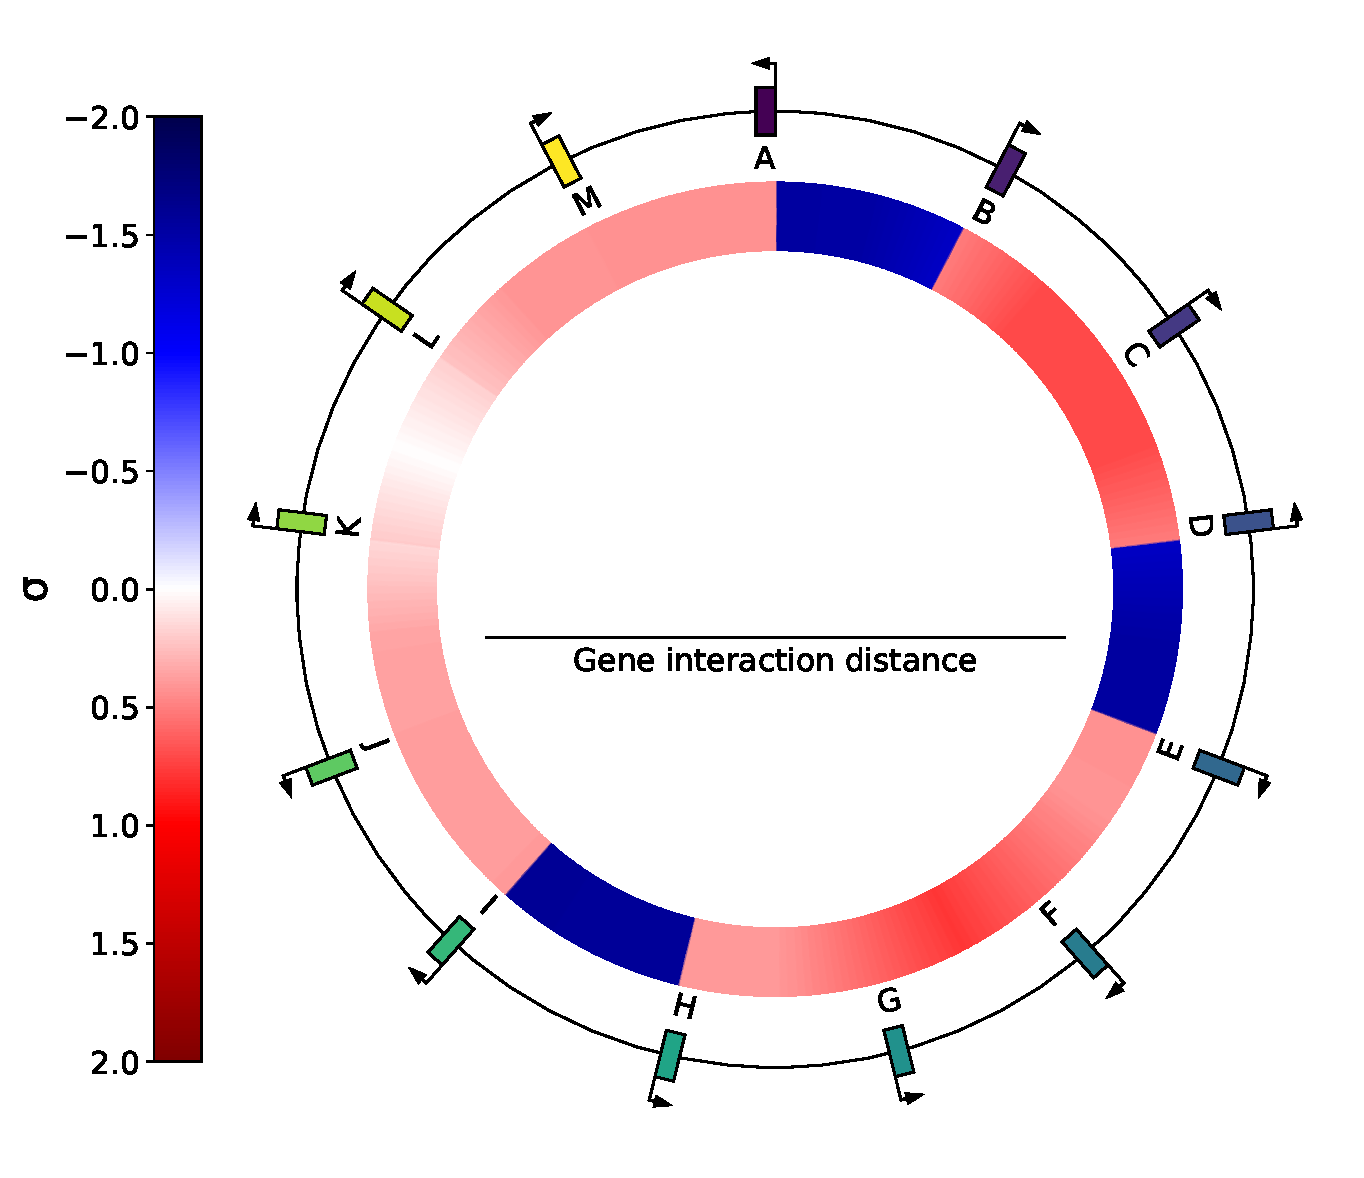
\includegraphics[width=\textwidth]{alife/img/13genes_genome.pdf}
\label{subfig:alife:13genes_genome}
\end{subfigure}
\begin{subfigure}[t]{0.56\textwidth}
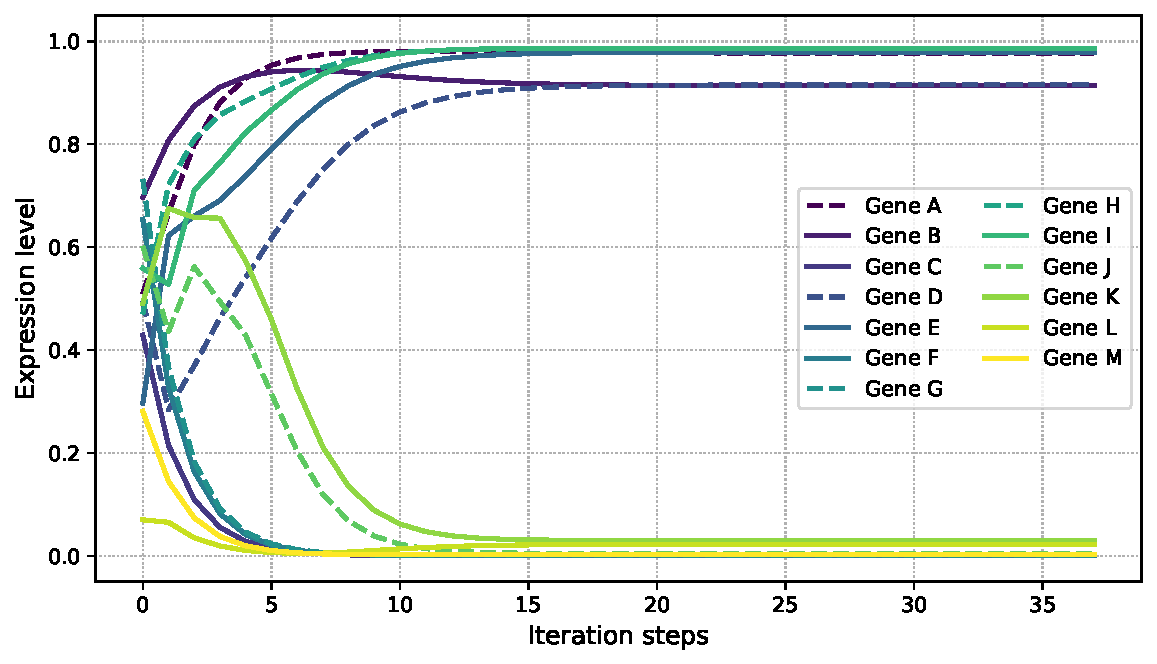
\includegraphics[width=\textwidth]{alife/img/13genes_expr_level.pdf}
\label{subfig:alife:13genes_expr}
\end{subfigure}
\caption[Example individual in the proof-of-concept model]{Left: genome (outer ring) and stable state level of supercoiling $\sigma$ (inner ring) of an example individual with 13 genes in the model.
Right: transcription levels of the individual's genes during the iterations of the fixed point computation, in an environment given by $\sigma_{env} = 0.05$.
Solid lines represent genes in forward orientation, and dashed lines represent genes in reverse orientation.}
\label{fig:alife:13genes}
\end{figure}

Figure~\ref{fig:alife:13genes} shows the genome (left, outer ring) of an example individual with a genome of 13,000 bp and $n=13$ genes evenly spaced along the genome, and with a basal supercoiling of $\sigma_{basal} = -0.06$.
The basal transcription level of each gene is randomly chosen between 0 and 1, and all the iterations of the fixed point algorithm that result in the final gene transcription levels are shown on the right.
In this individual, the non-linear effect of the interaction between neighboring genes is clearly visible.
Indeed, six genes (A, B, D, E, H, and I) end up at a high transcription rate at the fixed point (or solution) of the system, while the others end up at low transcription rates.
These activated genes can be grouped into 3 pairs (A and B, D and E, H and I), all of which are pairs of adjacent genes in divergent orientations.
Even though gene D has a low (around 0.3) basal transcription rate, it eventually reaches a high transcription state because of its positive interaction with gene E.
Conversely, genes F and G start with a high transcription rate, but are repressed by their neighbors H and E, and are therefore silenced as the system converges.
We can also observe complex behaviors in the model, as the gene expression levels pass through very different states during convergence to the solution.
Indeed, the transcription level of gene K initially increases due to its interaction with gene J, but both genes end up in a low transcription state, as they are inhibited by the very active gene I.
The final supercoiling level along the genome (left, inner ring) moreover demonstrates the effect of the transcription-supercoiling coupling on local supercoiling.
Highly transcribed genes, such as A and B, generate a large variation in the supercoiling level on their upstream and downstream sides, and the positive feedback loop between genes in divergent pairs is made clear by the very high negative value of the supercoiling level between each of the genes in these two pairs.


\subsection{Effect of the Environmental Supercoiling on Gene Activation Levels}
\label{sec:alife:env_model}

\begin{figure}[H]
\centering
\begin{subfigure}[t]{0.28\textwidth}
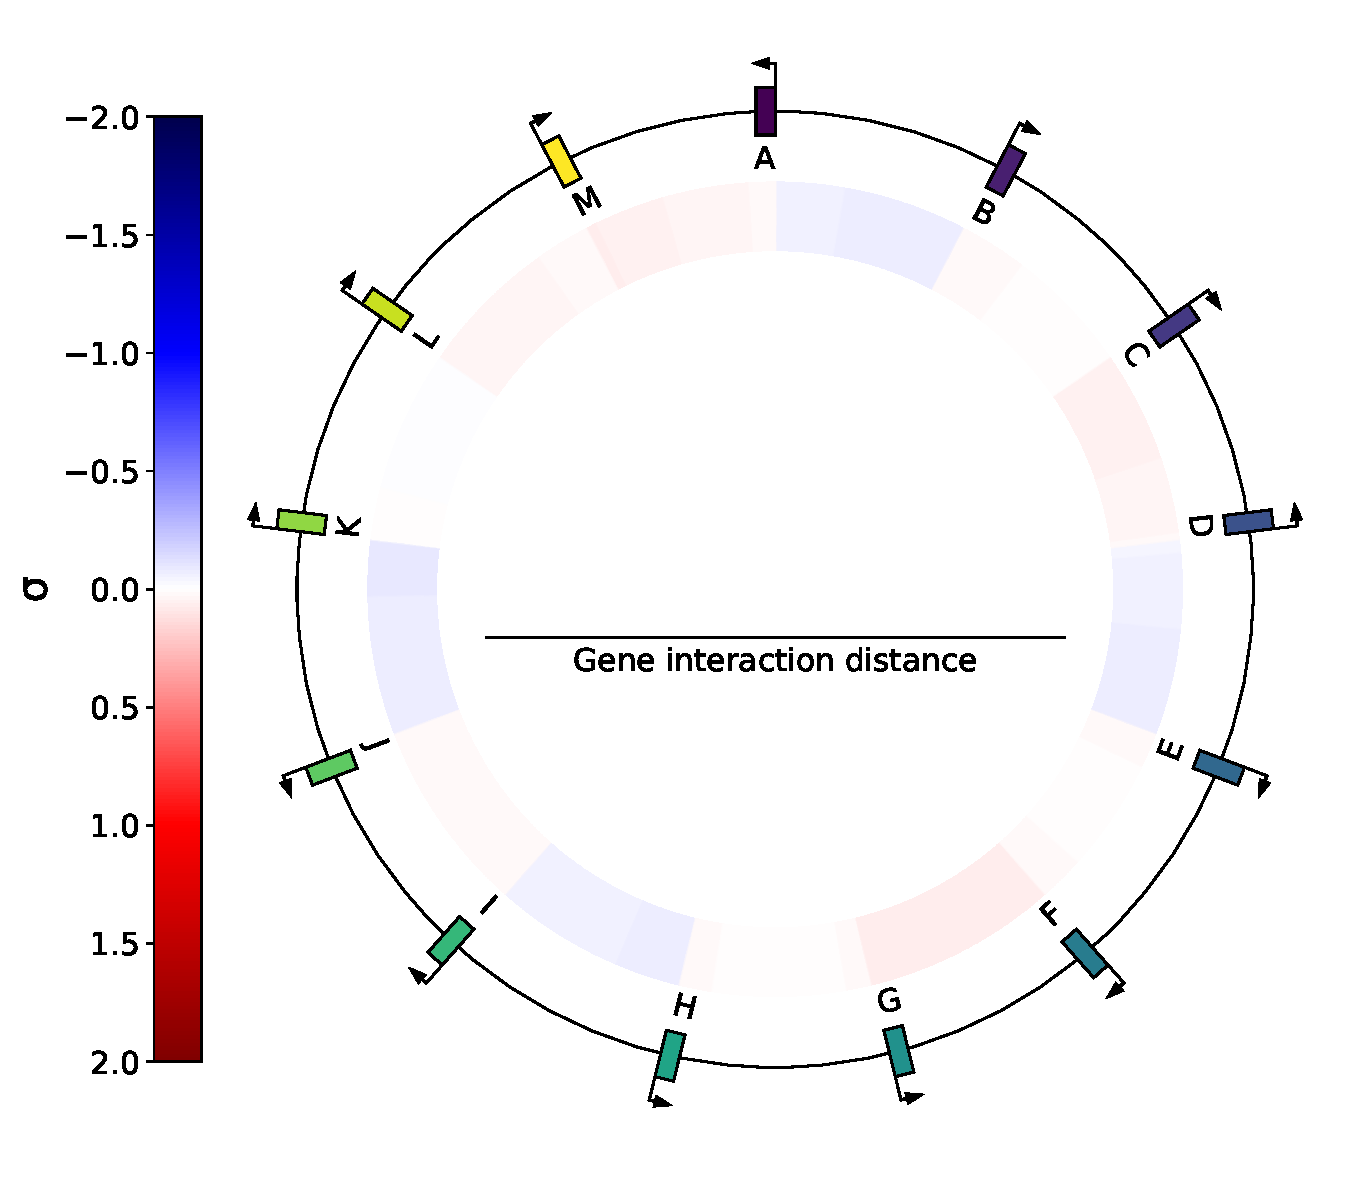
\includegraphics[width=\textwidth]{alife/img/13genes_genome_3.pdf}
\label{subfig:alife:genome_3}
\end{subfigure}
\hspace{-3mm}
\begin{subfigure}[t]{0.24\textwidth}
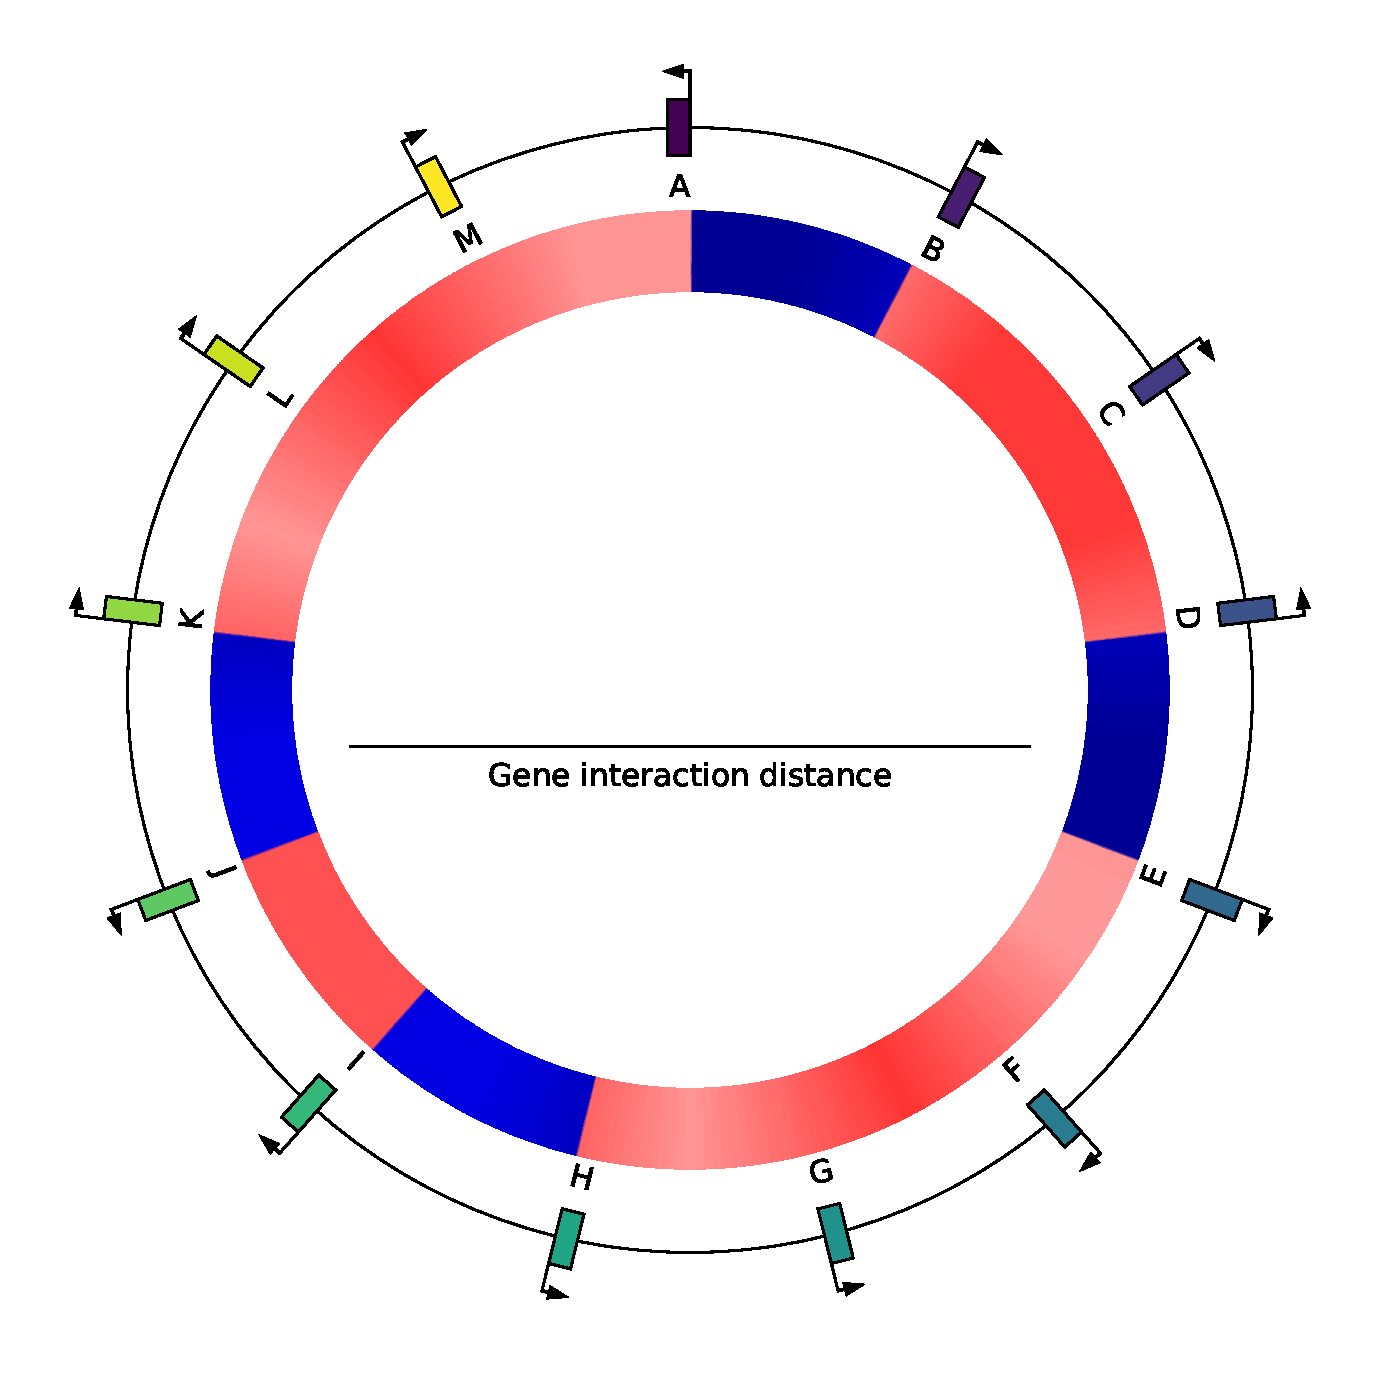
\includegraphics[width=\textwidth]{alife/img/13genes_genome_2.pdf}
\label{subfig:alife:genome_2}
\end{subfigure}
\hspace{-3mm}
\begin{subfigure}[t]{0.24\textwidth}
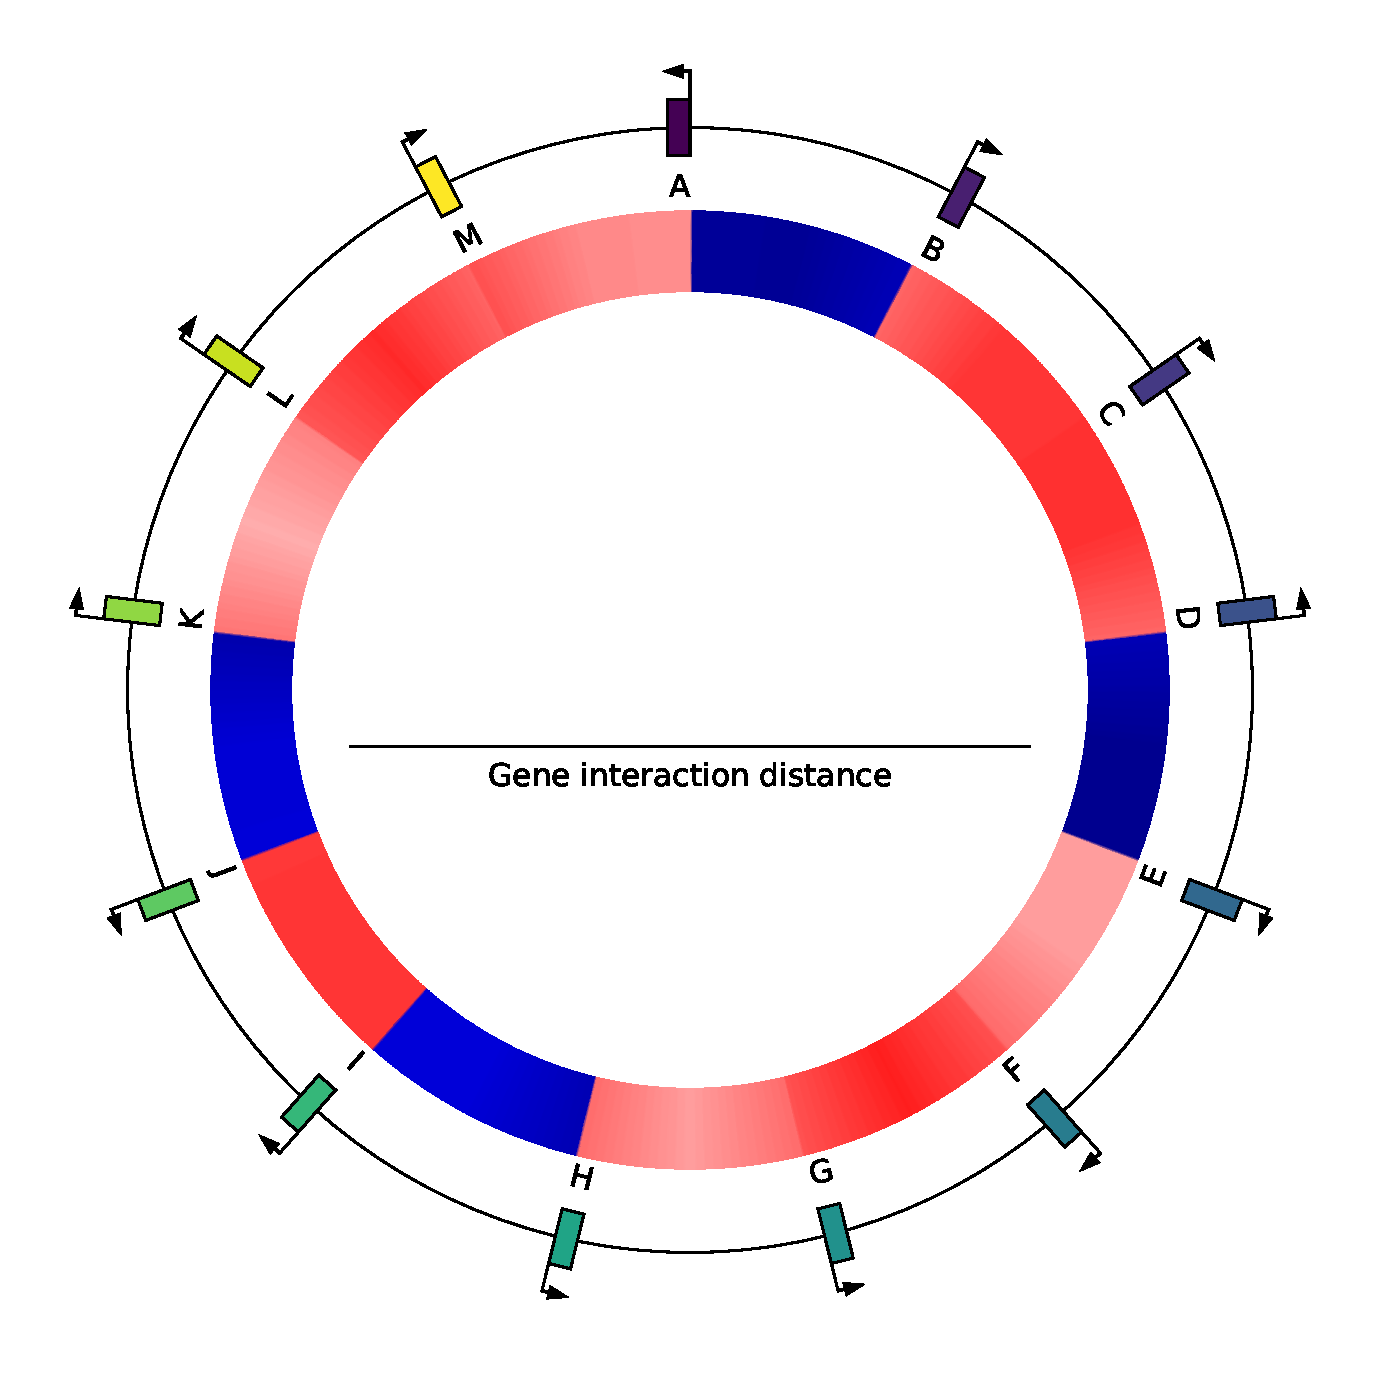
\includegraphics[width=\textwidth]{alife/img/13genes_genome_1.pdf}
\label{subfig:alife:genome_1}
\end{subfigure}
\hspace{-3mm}
\begin{subfigure}[t]{0.24\textwidth}
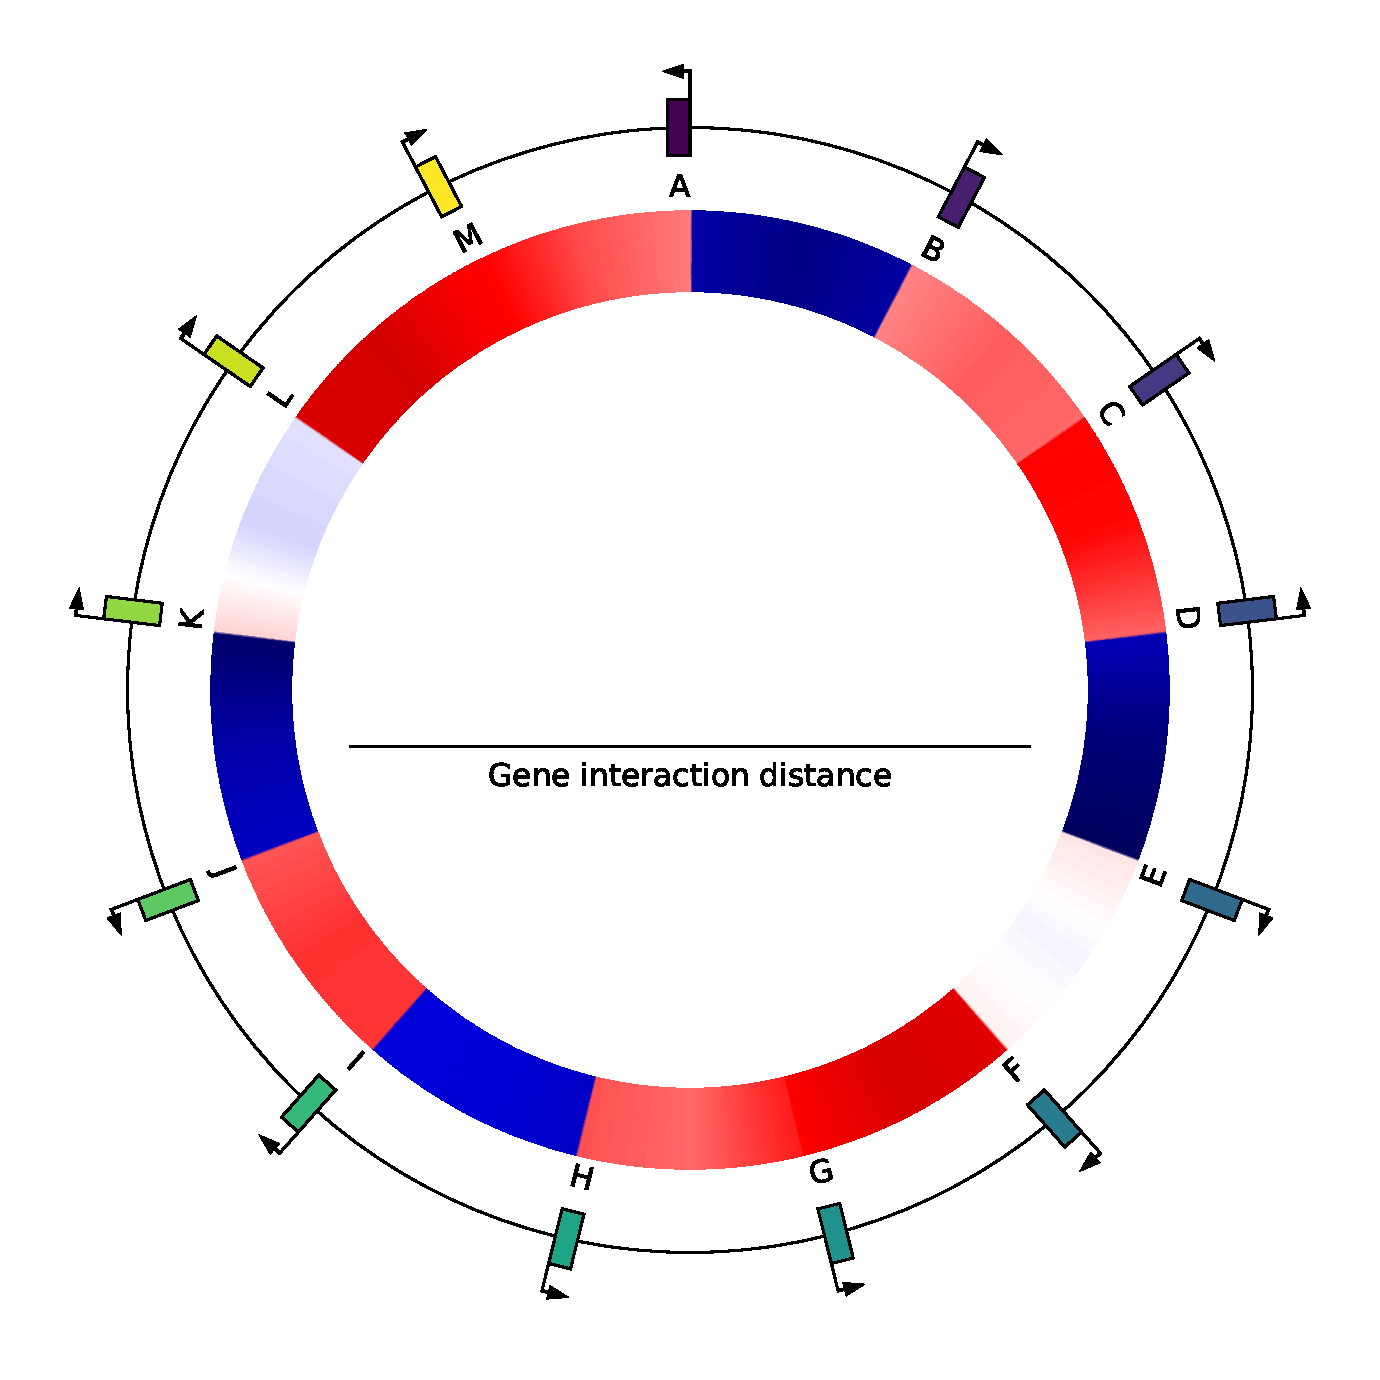
\includegraphics[width=\textwidth]{alife/img/13genes_genome_0.pdf}
\label{subfig:alife:genome_0}
\end{subfigure}
\vspace{-3mm}

\begin{subfigure}[t]{0.48\textwidth}
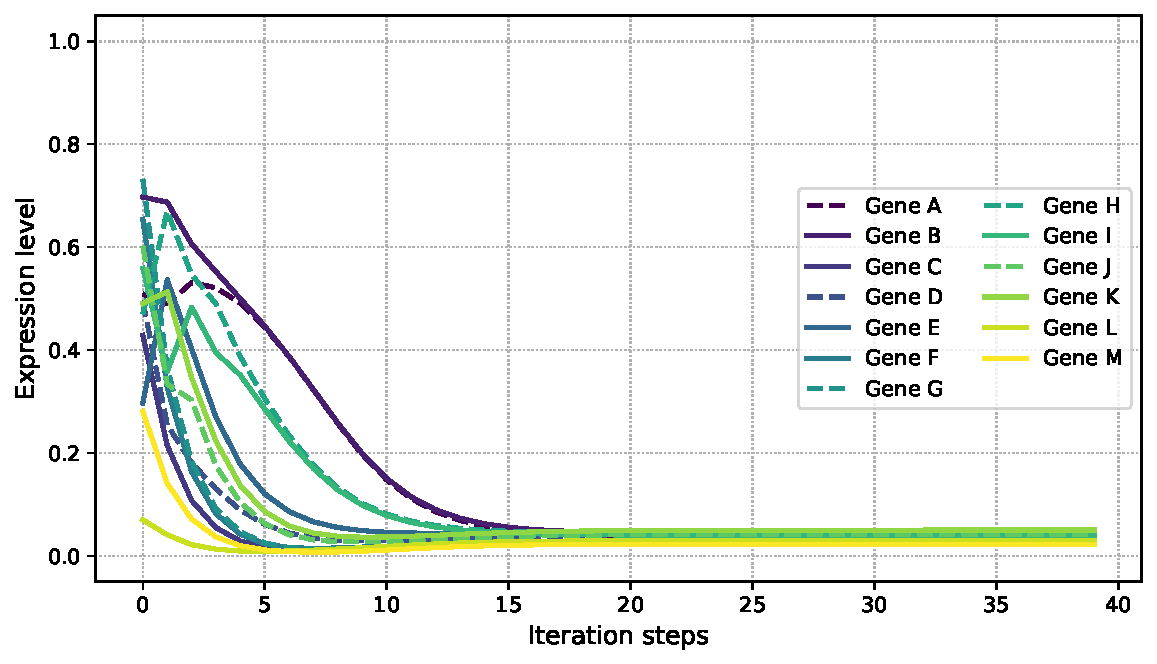
\includegraphics[width=\textwidth]{alife/img/13genes_sigma_3.pdf}
\label{subfig:alife:sigma_3}
\end{subfigure}
\begin{subfigure}[t]{0.48\textwidth}
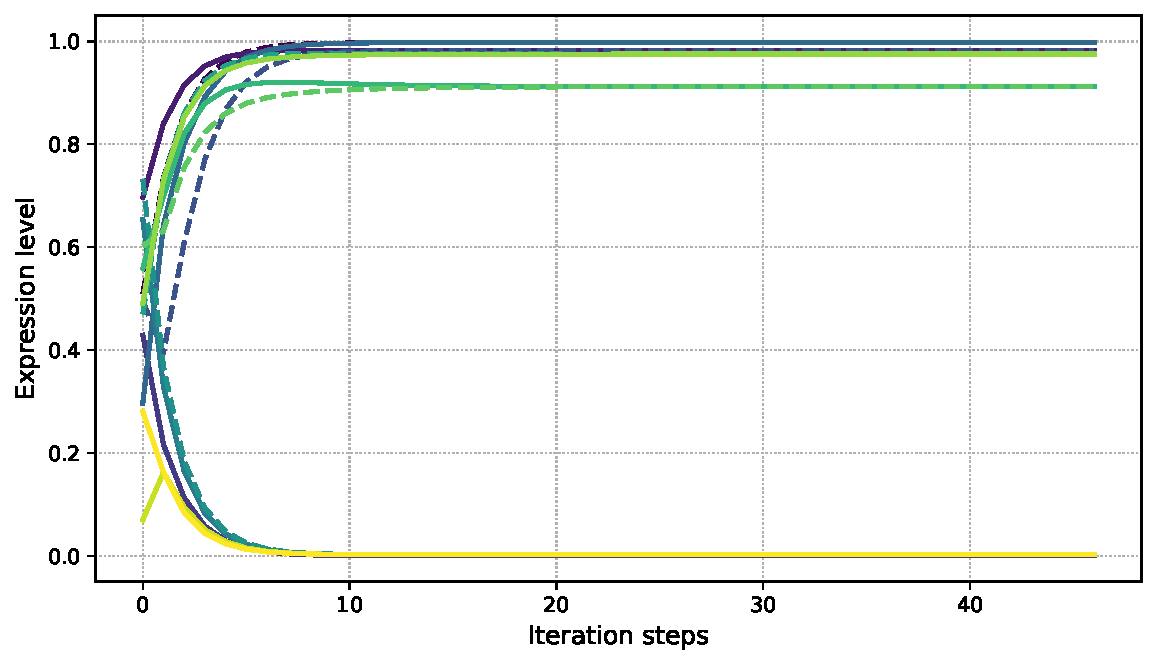
\includegraphics[width=\textwidth]{alife/img/13genes_sigma_2.pdf}
\label{subfig:alife:sigma_2}
\end{subfigure}
\vspace{-5mm}

\begin{subfigure}[t]{0.48\textwidth}
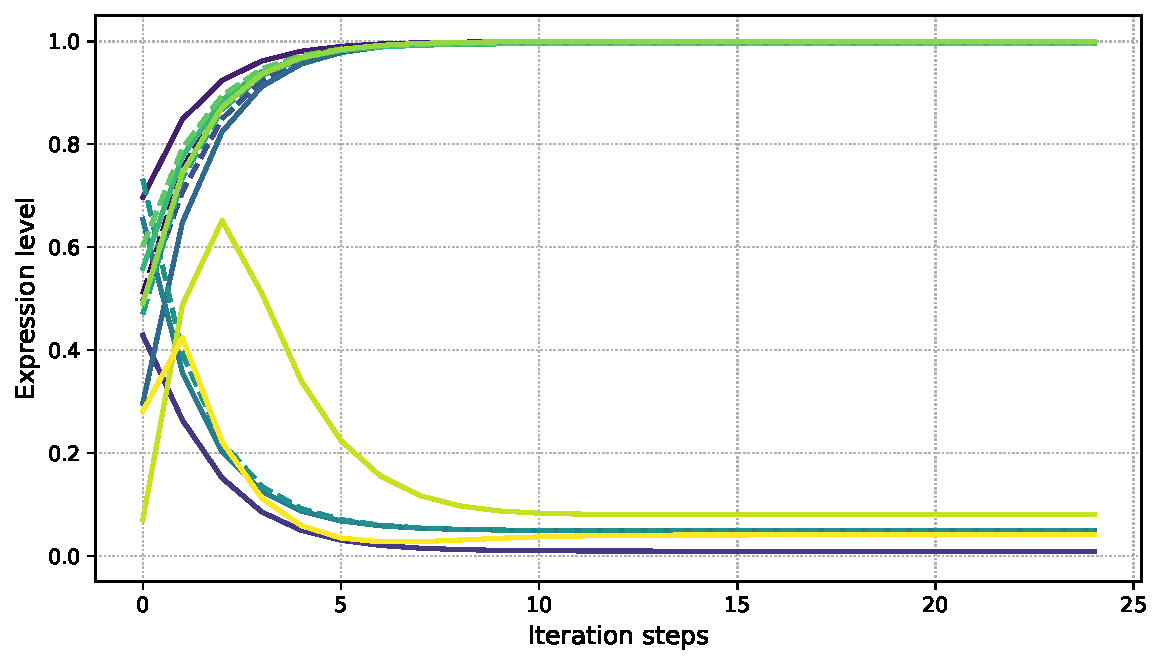
\includegraphics[width=\textwidth]{alife/img/13genes_sigma_1.pdf}
\label{subfig:alife:sigma_1}
\end{subfigure}
\begin{subfigure}[t]{0.48\textwidth}
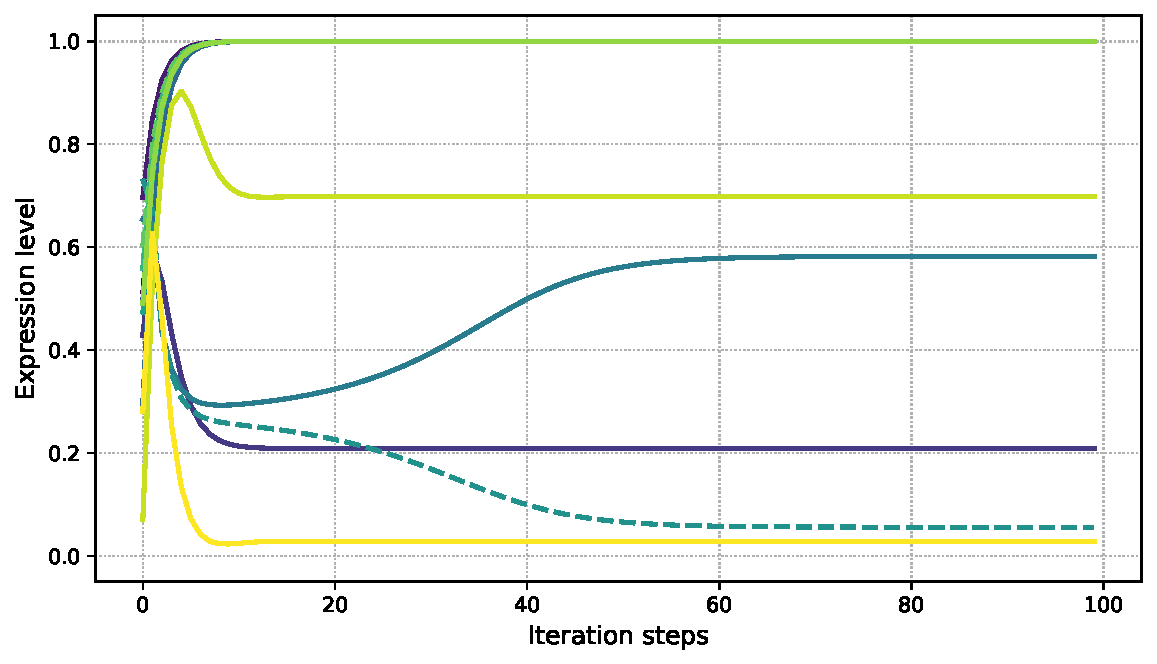
\includegraphics[width=\textwidth]{alife/img/13genes_sigma_0.pdf}
\label{subfig:alife:sigma_0}
\end{subfigure}
\caption[Influence of environmental supercoiling on the phenotype of the example individual in Figure~\ref{fig:alife:13genes}]{Influence of the environment supercoiling $\sigma_{env}$ on the stable state local supercoiling level (top row) and gene transcription levels (bottom rows) of the example individual.
From left to right and top to bottom: at $\sigma_{env} = 0.1$, no genes are activated ($e > 0.5$); at $\sigma_{env} = 0.0$ and at $\sigma_{env} = -0.1$, 8 genes are activated; at $\sigma_{env} = -0.2$, 10 genes are activated.
Lower values of $\sigma_{env}$ result in the activation of more genes, reflecting the \emph{in vivo} effect of higher negative supercoiling.}
\label{fig:alife:sigma_env}
\end{figure}

Figure~\ref{fig:alife:sigma_env} captures the influence of the environmental change in supercoiling $\sigma_{env}$ on the local supercoiling level due to the transcription-supercoiling coupling (top row) and on the repartition of genes between the activated and inhibited states (bottom rows), again using the example individual already shown in Figure~\ref{fig:alife:13genes}.
From left to right and top to bottom: at a high value of $\sigma_{env} = 0.1$, meaning that DNA is severely overwound compared to normal, no gene is activated (with an expression level $e > 0.5$) at all.
As the external influence of the environment on supercoiling decreases to $\sigma_{env} = 0$, corresponding to normal relaxation of DNA, and then to $\sigma_{env} = -0.1$, 8 out of the 13 genes of the individual reach an activated state.
Finally, for $\sigma_{env} = -0.2$, there is a strong environmental pressure towards high gene transcription levels, and most genes are indeed activated; however, even at this level of $\sigma_{env}$, some genes remain shut down, because of the high amount of positive supercoiling (in red) generated by the transcription of their neighbors.


\subsection{Influence of Relative Gene Positions on Gene Activation Levels}
\label{sec:alife:gene_pos}

\begin{figure}[H]
\centering
\begin{subfigure}[t]{0.42\textwidth}
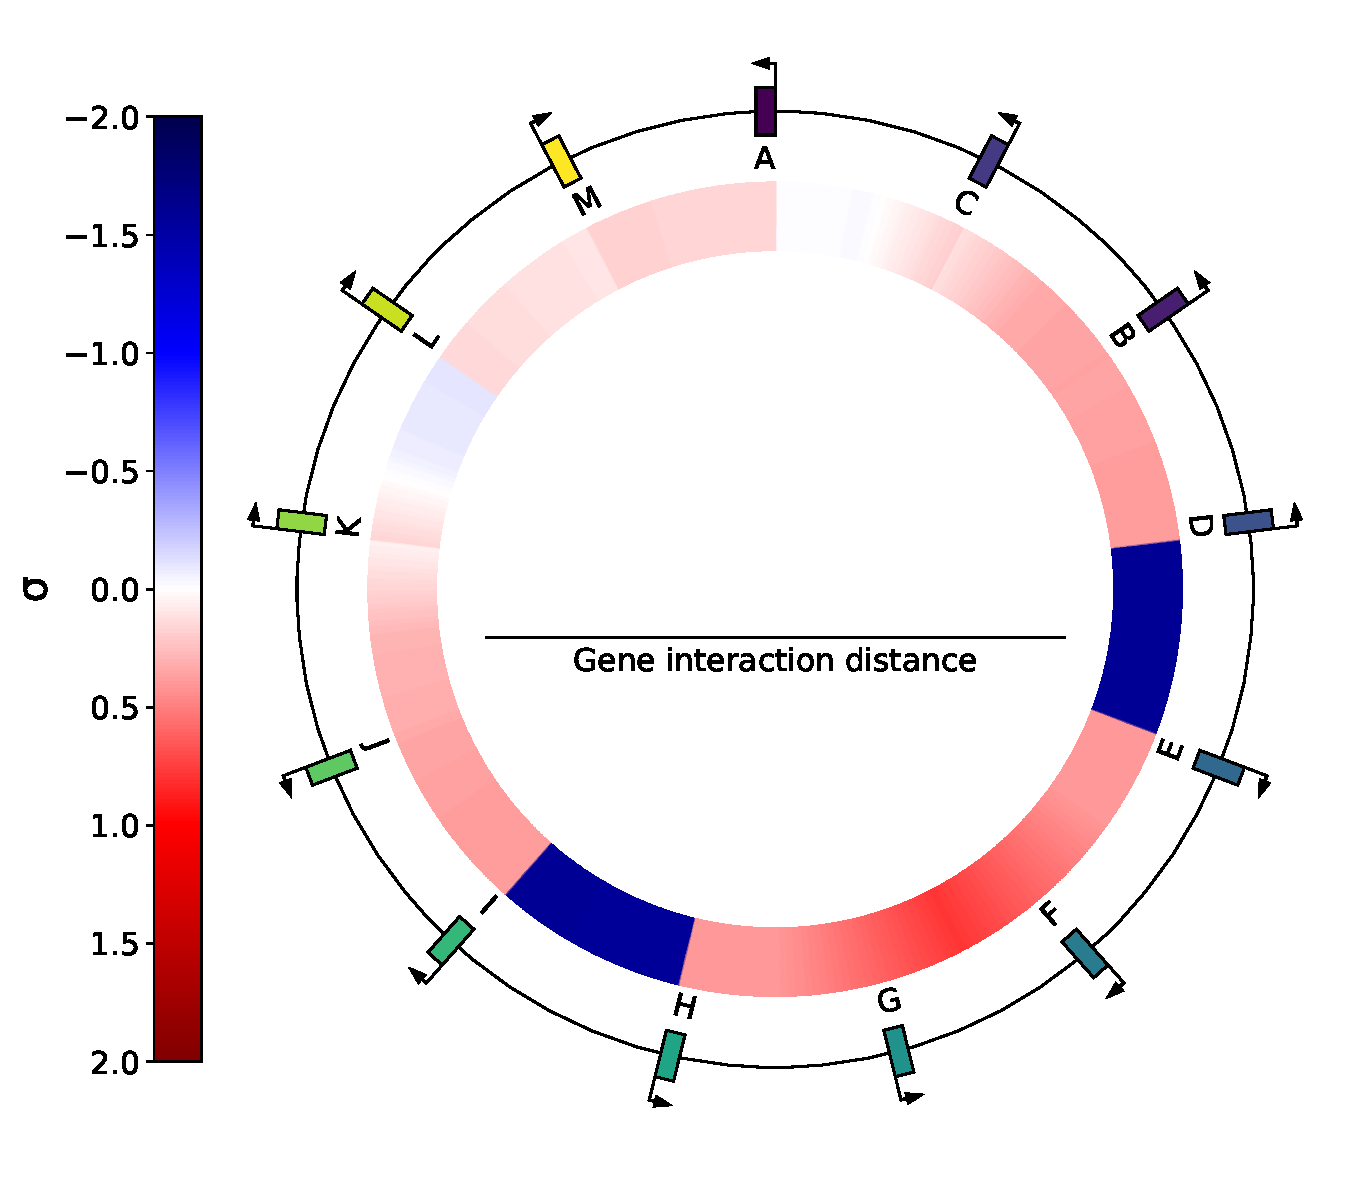
\includegraphics[width=\textwidth]{alife/img/inversion_genome.pdf}
\label{subfig:alife:inversion_genome}
\end{subfigure}
\begin{subfigure}[t]{0.56\textwidth}
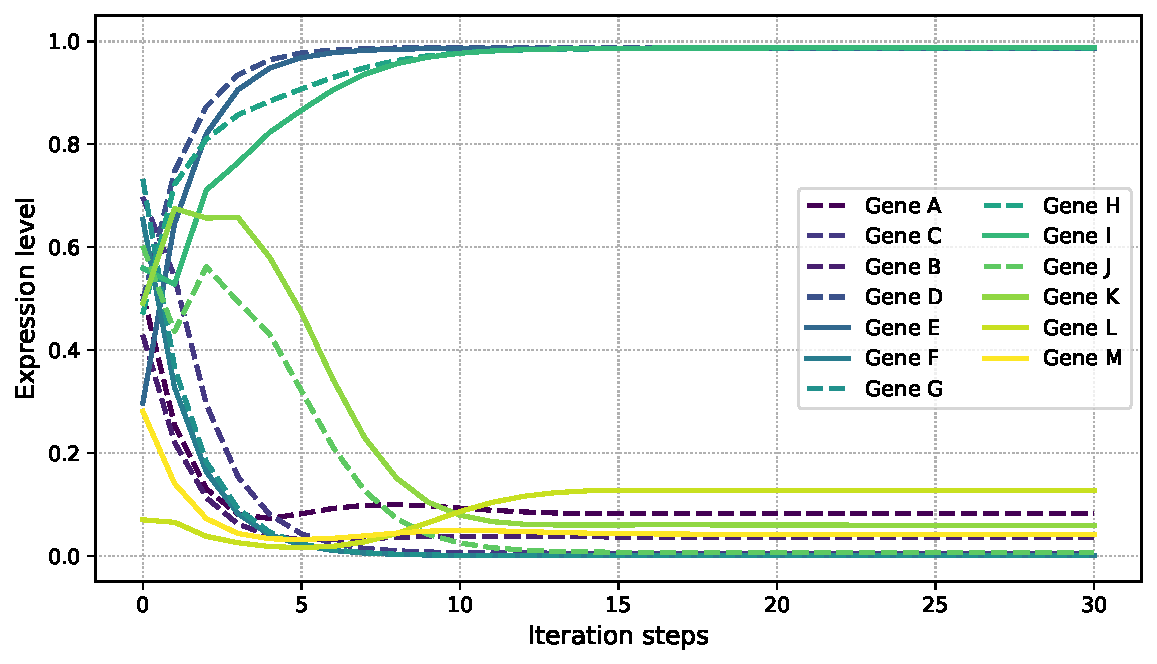
\includegraphics[width=\textwidth]{alife/img/inversion_expr_level.pdf}
\label{subfig:alife:inversion_expr}
\end{subfigure}
\caption[Effect of a genomic inversion on the example individual in Figure~\ref{fig:alife:13genes}]{Genome, local supercoiling and gene expression levels of a new individual obtained from the individual in Figure~\ref{fig:alife:13genes} by switching the positions and orientations of genes B and C.}
\label{fig:alife:inversion}
\end{figure}

Figure~\ref{fig:alife:inversion} again shows the local supercoiling and gene expression levels of the individual in Figure~\ref{fig:alife:13genes}, after reversing the positions and orientations of genes B and C.
This is an example of a genomic inversion, which will be presented in further detail in section~\ref{sec:inversion}.
The starting point of this inversion falls between genes A and B and its end point between genes C and D; this results in the reversal of segment [BC] relative to the rest of the genome.
Here, we can see that the diverging orientation that was present between genes A and B has vanished, replaced by a set of genes in colinear orientation, from A to D.
This genomic reorganization results in the loss of the activation of genes A and B, as gene B is now more strongly inhibited by gene D due to its closer genomic location, and as genes A and B are not in a positive feedback loop -- due to diverging orientations -- any longer; only the pairs of genes D and E, and H and I, remain activated.

Based on these observations, we can confirm that in our model, the transcription"=supercoiling coupling generates complex networks of genome-wide interactions between genes, and that these networks directly depend on the architecture of the genome.


\section{An Evolutionary Genome-Wide Model of the Transcription-Supercoiling Coupling}
\sectionmark{An Evolutionary Genome-Wide Model of the TSC}
\label{sec:alife:evol_model}

After evidencing that transcriptional activity depends on the organization of the genome, we now question to which extent evolution can simultaneously leverage the organization of the genome and the transcription-supercoiling coupling in order to adapt gene regulatory activity to different environments.
Indeed, as has been observed in \emph{Dickeya dadantii}~\citep{muskhelishvili2019}, different phenotypes can evolve as a response to different supercoiling levels induced by the environment, and the transcription-supercoiling coupling could play a role in enabling the existence of this reaction norm.

In this section, we expand our model into an evolutionary simulation.
At each generation of the simulation, all individuals are evaluated and their fitness values are computed, based on their gene transcription levels.
Then, the individuals of the new generation are chosen by picking their ancestor from the current generation, with a probability proportional to the ancestor's fitness.
The model is panmictic, meaning that any individual in the population can be chosen as the ancestor of any new individual.
Finally, during replication, the genome of each new individual stochastically undergoes a number of mutations, before the new individual is evaluated again; importantly, these mutations do not impact genes themselves, but only the spatial organization of the genome: gene orientations, syntenies, and intergenic distances.

\subsection{Evolutionary Model: Evolution in Two Separate Environments}

We model the evolution of populations of individuals that experience two different environments, named A and B.
Each environment is defined by its value of $\sigma_{env}$, respectively $\sigma_A$ and $\sigma_B$, which represent the change in the supercoiling level due to the environment~\citep{dorman2016}.
In order to have environments with distinct effects, we choose a value of $\sigma_A = 0.1$, for which isolated genes are effectively inhibited (as in the top-left panel of Figure~\ref{fig:alife:sigma_env}), and a value of $\sigma_B = -0.1$, for which some but not all genes are activated (bottom-left panel).

We separate genes into three classes, based on the environments in which they must be activated: either in both environment A and environment B (\emph{AB} genes), only in environment A (\emph{A} genes), or only in environment B (\emph{B} genes).
These classes allow us to define optimal phenotypes for both environments: in environment A, both \emph{A} and \emph{AB} genes should be activated, whereas \emph{B} genes should be inhibited.
Conversely, in environment B, only \emph{B} and \emph{AB} genes should be activated, but not \emph{A} genes.


\subsection{Fitness}

In order to compute the fitness of an individual, we define an optimal phenotype $\tilde{e}^A$ (resp. $\tilde{e}^B$), corresponding to the vector of the expected expression level $\tilde{e}^A_i$ for each gene $i$ in environment A (resp. environment B).
We choose an expected expression level of $\tilde{e} = 1$ for genes that should be activated, which corresponds to the maximum possible expression level of a gene in our model.
Similarly, we choose $\tilde{e} = 0$ for genes that should be inhibited, which is the minimum expression level that is attainable.
Then, in each environment, we compute the gap $g_A$ (resp. $g_B$), or average square distance of the individual's gene transcription levels $e^A$ (the vector constituted by the transcription level $e^A_i$ of each gene $i$) to the optimal levels $\tilde{e}^A$ (resp. $e^B$ and $\tilde{e}^B$).
The gap $g_A$ is computed as follows:

\begin{equation}
g_A(e^A) = \frac{1}{n} \sum_{i=1}^{n} (e^A_i - \tilde{e}^A_i)^2
\label{eq:alife_gap}
\end{equation}

The gap $g_B$ is computed in the same way.
Finally, we compute the fitness of the individual by summing the gap in each environment, and applying an exponential scaling: $f = e^{-k (g_A + g_B)}$, where $k$ is a scaling factor representing the selection pressure.
A higher value of $k$ means that well-adapted individuals, those which have a smaller gap, will have an even higher fitness value compared to other individuals; we typically use $k=50$, meaning that a small decrease in the gap compared to other individuals yields a large reproductive advantage.


\subsection{Mutational Operator: Genomic Inversions}
\label{sec:inversion}

We introduce only one kind of mutation in our model, which is genomic inversions: we choose two breakpoints randomly on the genome, and reverse the genomic content between these points.
Genes are then reinserted in the genome in the opposite orientation and order, taking care to update all intergenic distances appropriately.
Note that in our model, genes have a length of zero and the breakpoints can therefore not fall inside a gene.
Moreover, an inversion has no effect if both breakpoints fall between two neighboring genes (as only an intergenic region would be affected), but can impact any number of genes otherwise.
Genomic inversions hence affect gene syntenies and orientations, and therefore affect gene expression levels as presented in subsection~\ref{sec:alife:gene_pos}.
When mutating a genome during reproduction, we draw the number of inversions $k$ to perform from a Poisson law with parameter $\lambda = 2$, giving an average of 2 inversions between an individual and its ancestor; the probability of not undergoing any mutations is $P(k=0) = e^{-\lambda} \approx 0.136$.

\begin{figure}[H]
\centering
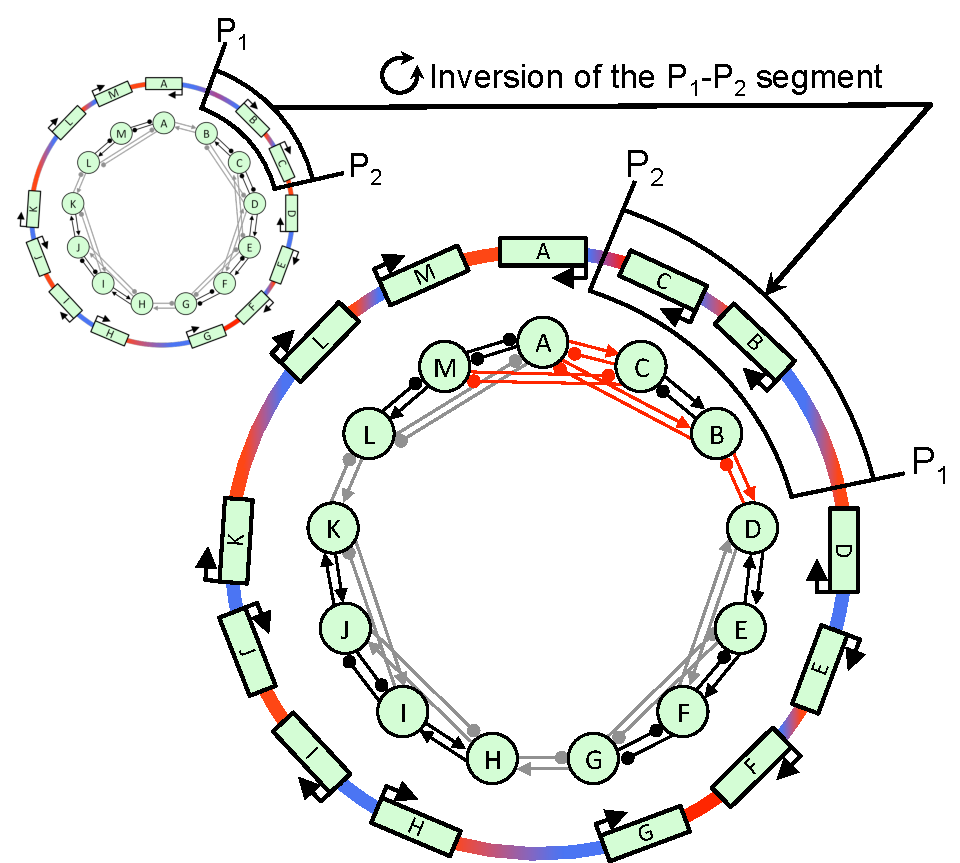
\includegraphics[width=0.8\textwidth]{alife/img/genome_inversion.pdf}
\caption[Effect of an inversion on the hand-drawn genome in Figure \ref{fig:alife:network}]{Result of the inversion of a genomic segment containing genes B and C from the individual presented in Figure~\ref{fig:alife:network}.
The gene interactions which have changed due to the inversion are drawn in red.
This illustration genome corresponds to the actual individual in our model presented in Figure~\ref{fig:alife:inversion}.}
\label{fig:alife:genome_inv}
\end{figure}

Figure \ref{fig:alife:genome_inv} presents a genome obtained by performing an inversion on the genome shown in Figure~\ref{fig:alife:network}.
As a result of this inversion, genes B and C have been switched from the forward to the backward orientation, and the intergenic distances between A and C on the one hand, and B and D on the other hand, have been modified; however, the relative orientation of B and C, and hence their interaction subnetwork, remain unchanged.
This results in changes to the gene interaction network: instead of mutual activation between genes A and B and mutual inhibition between genes C and D, all four genes now lie in colinear orientations, in which each of these genes activates its upstream neighbor but represses its downstream neighbor.

\subsection{Experimental Setup and Parameter Values}

We initialized the simulation with a clonal population of $N=100$ copies of an initial individual with the following genome: 60 genes in random orientations, uniformly distributed along a 60,000 bp genome, and equally divided between the \emph{AB}, \emph{A} and \emph{B} classes.
We chose a maximum interaction distance of $d_{max} = 2500$, meaning that each gene initially interacts with its 2 closest neighbors in each direction through the transcription-supercoiling coupling.
Note that as inversions may change intergenic distances, genes can move closer or further apart during evolution.
We set the basal supercoiling level $\sigma_{basal}$ to the average supercoiling level in \emph{E. coli} of -0.06~\citep{crozat2005}, and $\sigma_0$ to $-0.06$ as well, so that in the absence of other sources of supercoiling (either environmental or through the coupling), the default activity level of a gene is 0.5.
Finally, we set $c = 0.3$, in order to have comparable values for the variations in supercoiling due to the environment and due to the transcription-supercoiling coupling, and $\epsilon=0.03$, so that the variations in supercoiling have a qualitatively mild effect on gene expression.

In order to run the simulations, we evolved 15 different populations for 250,000 generations; the simulation lasted for approximately 48h on a computer with Intel Xeon E5-2640 v3 @ 2.60GHz CPUs, using around 100 MB of RAM per replicate.
All the data from the experiment is available online on the \href{https://doi.org/10.5281/zenodo.6556310}{Zenodo} platform.

\subsection{Adaptation of Gene Expression Levels to Different Environments}

Figure~\ref{fig:alife:mean_activ} summarizes the differences in the proportion of activated genes for each of the three sets of genes, between environments A and B, averaged over the 15 repetitions.
In the figure, we consider a gene to be activated if its activity at the end of the lifecycle is over $0.5$, and we look at the average proportion of activated genes in the best individual of every replica.
Let us recall that the evolutionary target for \emph{AB} genes is an expression level of 1 in both environments, for \emph{A} genes an expression level of 1 in environment \emph{A} and 0 in \emph{B}, and vice-versa for \emph{B} genes.
After 250,000 generations of evolution, individuals have acquired genomes that allow all \emph{AB} genes to be activated in both environments, and that allow all \emph{B} genes to be activated in environment B and inhibited in environment A.
On average, over 60\% of \emph{A} genes are activated in environment A, which imposes a positive change in supercoiling ($\sigma_A = 0.1$) and makes gene activation harder.
Conversely, less than 5\% of \emph{A} genes are activated in environment B, in which gene activation is easier ($\sigma_B = -0.1$).
The final expression levels of \emph{A} genes therefore show that specific sets of genes can be activated by the transcription-supercoiling coupling despite environmental hurdles.

\begin{figure}[H]
\centering
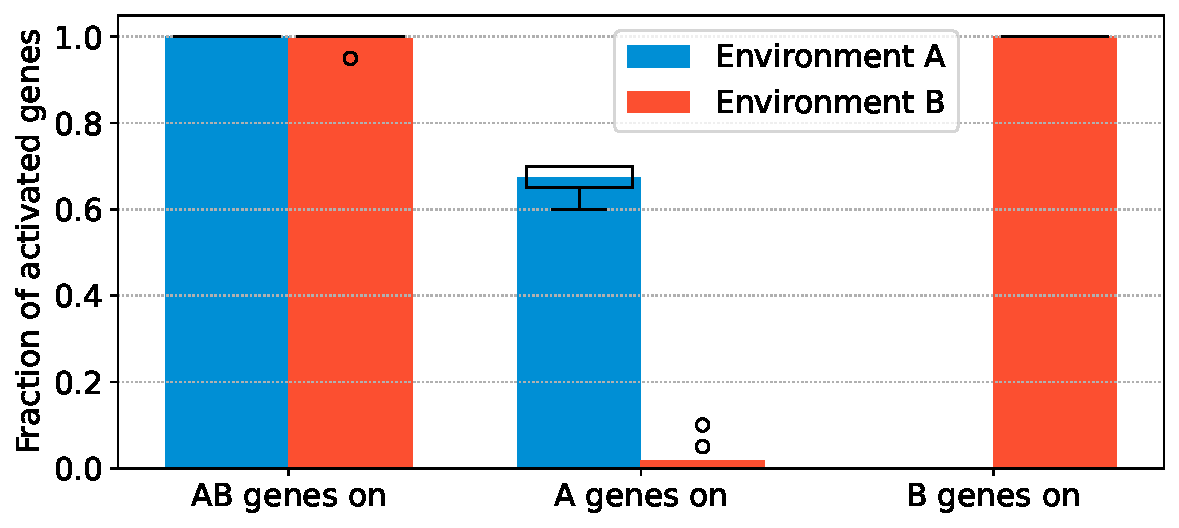
\includegraphics[width=0.8\textwidth]{alife/img/mean_activation.pdf}
\caption[Fraction of activated genes of each type at the end of evolution in the proof-of-concept model]{Fraction of activated genes of each type in each environment at the end of the lifecycle, averaged over the best individuals in the last generation of each replica.
The boxplots represent the median and quartiles, and the dots flier data points.
For \emph{A} genes and \emph{B} genes, activation levels differ depending on the environment: $p$-value $2.40\times10^{-17}$ for \emph{A} genes, and $p$-value $<1\times10^{-25}$ for \emph{B} genes (Student's $t$-test for dependent samples).}
\label{fig:alife:mean_activ}
\end{figure}

Furthermore, in each of the 15 replicates, the fitness of the best individual in the population increases continuously over the course of evolution, as shown in Figure~\ref{fig:alife:fitnesses}.
As their respective fitness keeps increasing until the end of the simulation, this suggests that fitter phenotypes remain reachable through further evolution by genomic rearrangements.
The rhythm of evolution is however progressively slower and slower (note the logarithmic time scale in the figure), as the pool of available favorable mutations decreases.

\begin{figure}[H]
\centering
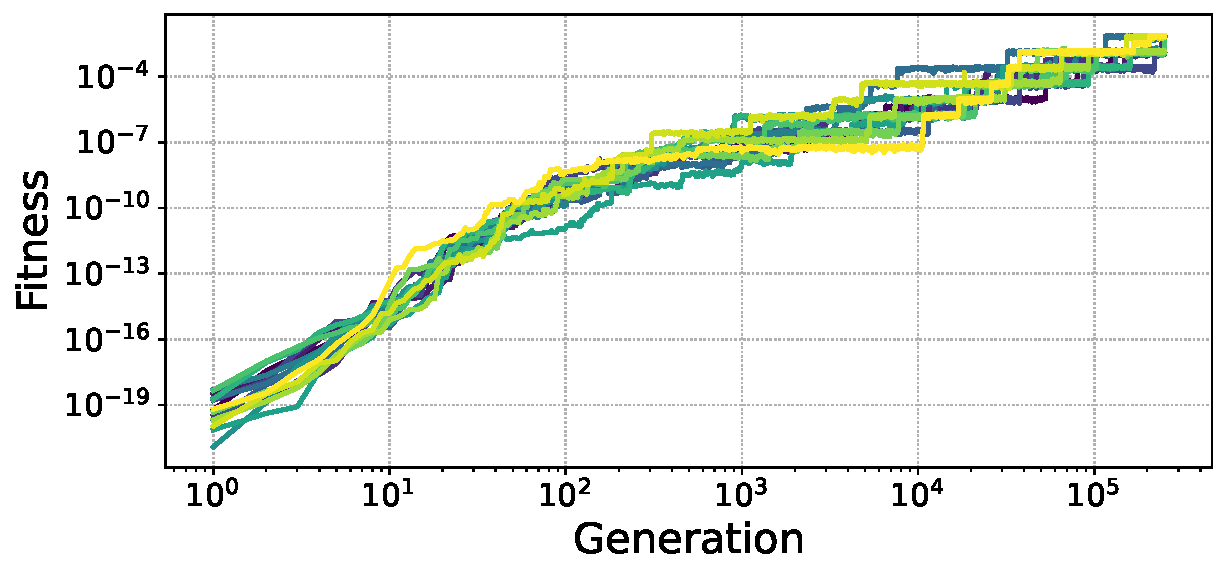
\includegraphics[width=0.8\textwidth]{alife/img/all_fitness.pdf}
\caption[Fitness of every replicate during evolution in the proof-of-concept model]{Evolution of the fitness of the best individual of each replicate at every generation.}
\label{fig:alife:fitnesses}
\end{figure}

Finally, details of the evolution of one of the 15 replicate populations are shown in Figure~\ref{fig:alife:evolution}.
We can first see that the number of activated \emph{AB} genes of the best individual at each generation quickly rises to 20 (out of 20 genes of that type) in both environment A and environment B; this shows that evolving a phenotype that is resistant to environmental perturbations, having genes that are always activated, is easy in the model.
For \emph{A} genes and \emph{B} genes, we observe an asymmetric tendency during the course of evolution towards activation in the target environment, and inhibition in the opposite environment.
However, the difference in the number of activated \emph{B} genes between environment A and environment B is much higher than for \emph{A} genes.
As already mentioned above, this asymmetry comes from the different requirements expected of \emph{A} genes and \emph{B} genes: gene activation is easier in environment B than in environment A, as it is easier for a gene to become activated in an environment with a lower overall supercoiling level.
\emph{A} genes therefore have to be activated in a harder environment, and inhibited in a simpler environment, whereas \emph{B} genes have to do the opposite.

\begin{figure}[H]
\centering
\begin{subfigure}[t]{0.8\textwidth}
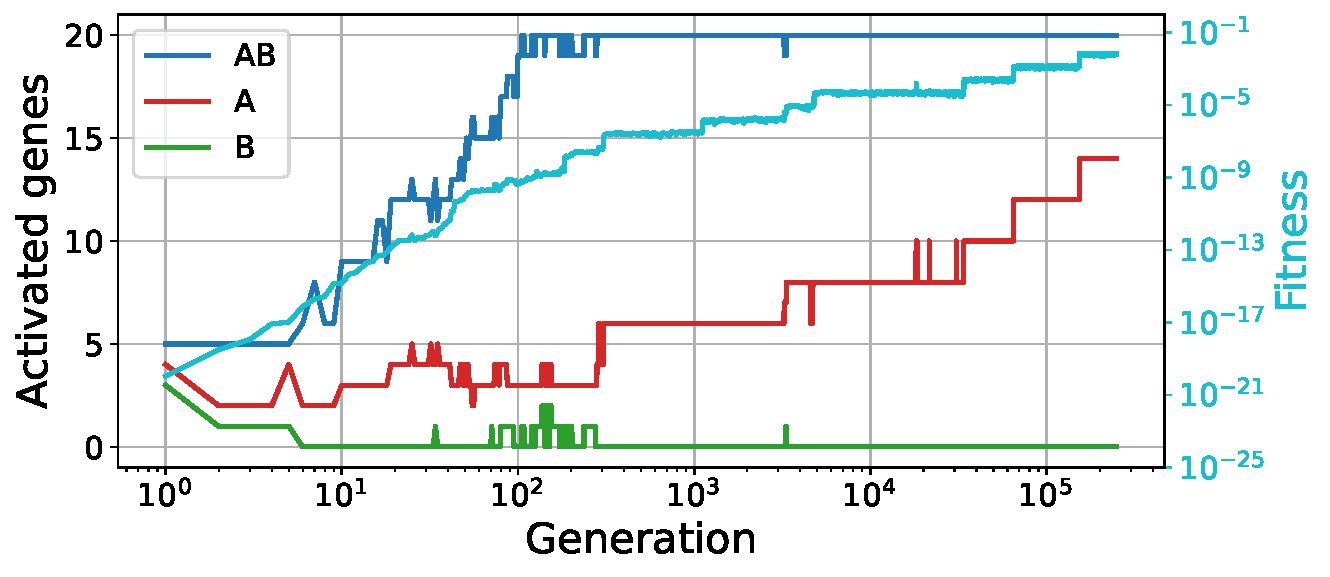
\includegraphics[width=\textwidth]{alife/img/rep_13_env_A.pdf}
\label{subfig:alife:env_A}
\end{subfigure}

\begin{subfigure}[t]{0.8\textwidth}
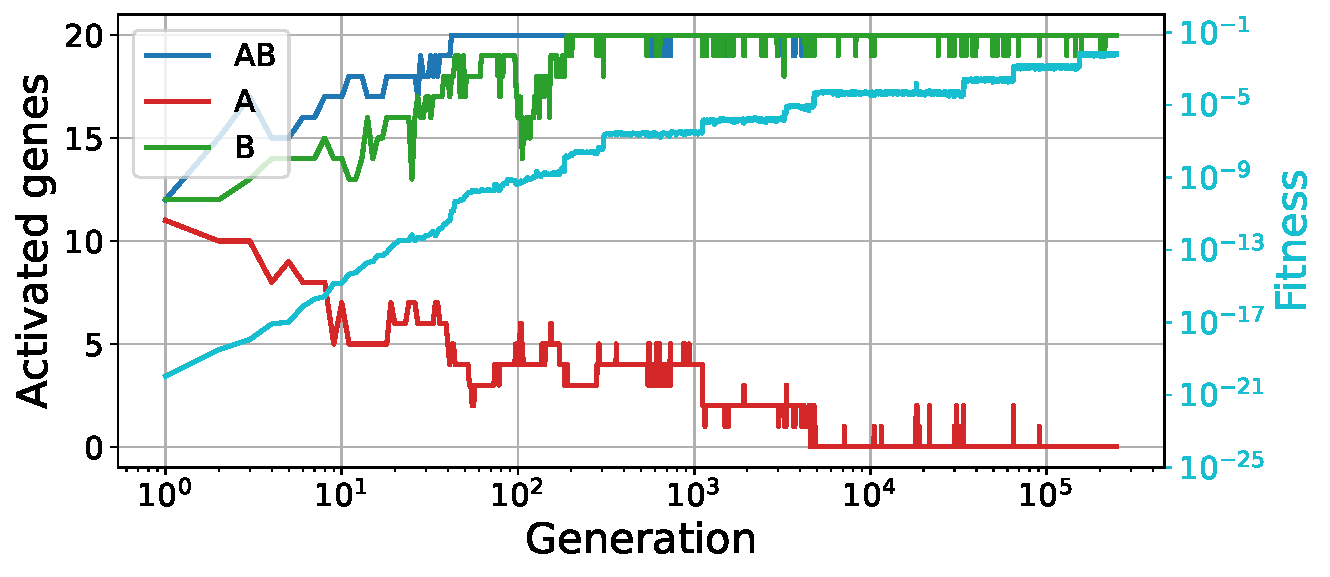
\includegraphics[width=\textwidth]{alife/img/rep_13_env_B.pdf}
\label{subfig:alife:env_B}
\end{subfigure}

\caption[Number of activated genes during evolution in one of the replicates in the proof-of-concept model]{Number of activated genes of each type and fitness of the best individual at every generation of replicate 13, with a population size of $N=100$, for 250,000 generations.
The number of active \emph{AB} genes increases until it reaches 20, in both environment A (top) and environment B (bottom).
The number of active \emph{A} (resp. \emph{B}) genes increases in environment A (resp. B) and decreases in environment B (resp. A) over time, thus converging towards their evolutionary target.}
\label{fig:alife:evolution}
\end{figure}

This is shown in more detail in Figure~\ref{fig:alife:best_indiv}, which shows the supercoiling level and gene activation levels of the best individual of the last generation of replicate 13, in both environments.
The phenotypes displayed in each environment present clearly distinct gene expression patterns.
In environment A (top), nearly all genes converge directly towards their final state, whereas in environment B (bottom), most \emph{A} genes (in red) and some \emph{B} genes (in green) show a complex trajectory of activation levels before reaching their stable state.
Moreover, genomic domains with markedly different supercoiling levels emerge through the transcription-supercoiling coupling, with both very overwound and very underwound zones.
These domains also show qualitatively different responses to different environments: in some domains, the supercoiling level is very similar (around gene 0, gene 15 or gene 55 for example), while in others supercoiling is completely different in each environment (between genes 20 and 35).
This shows the plasticity of the response to environmental change at the local supercoiling level.

\begin{figure}[H]
\centering
\begin{subfigure}[t]{0.42\textwidth}
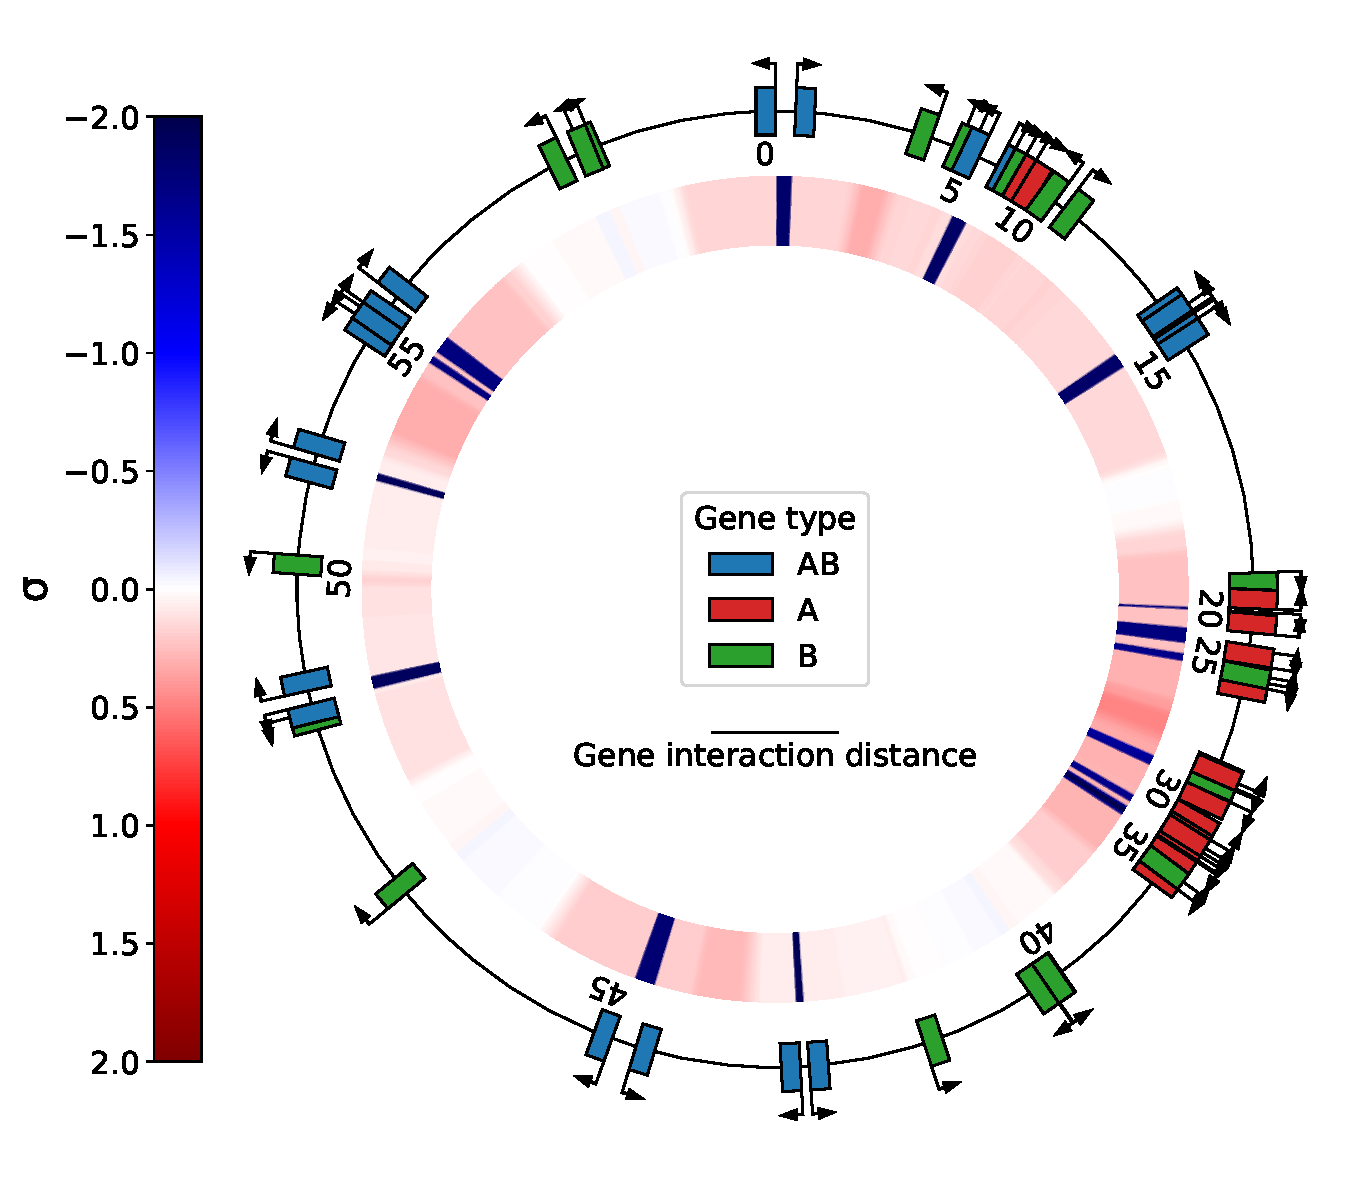
\includegraphics[width=\textwidth]{alife/img/genome_and_tsc_rep13_env_A.pdf}
\label{subfig:alife:best_genome_A}
\end{subfigure}
\begin{subfigure}[t]{0.56\textwidth}
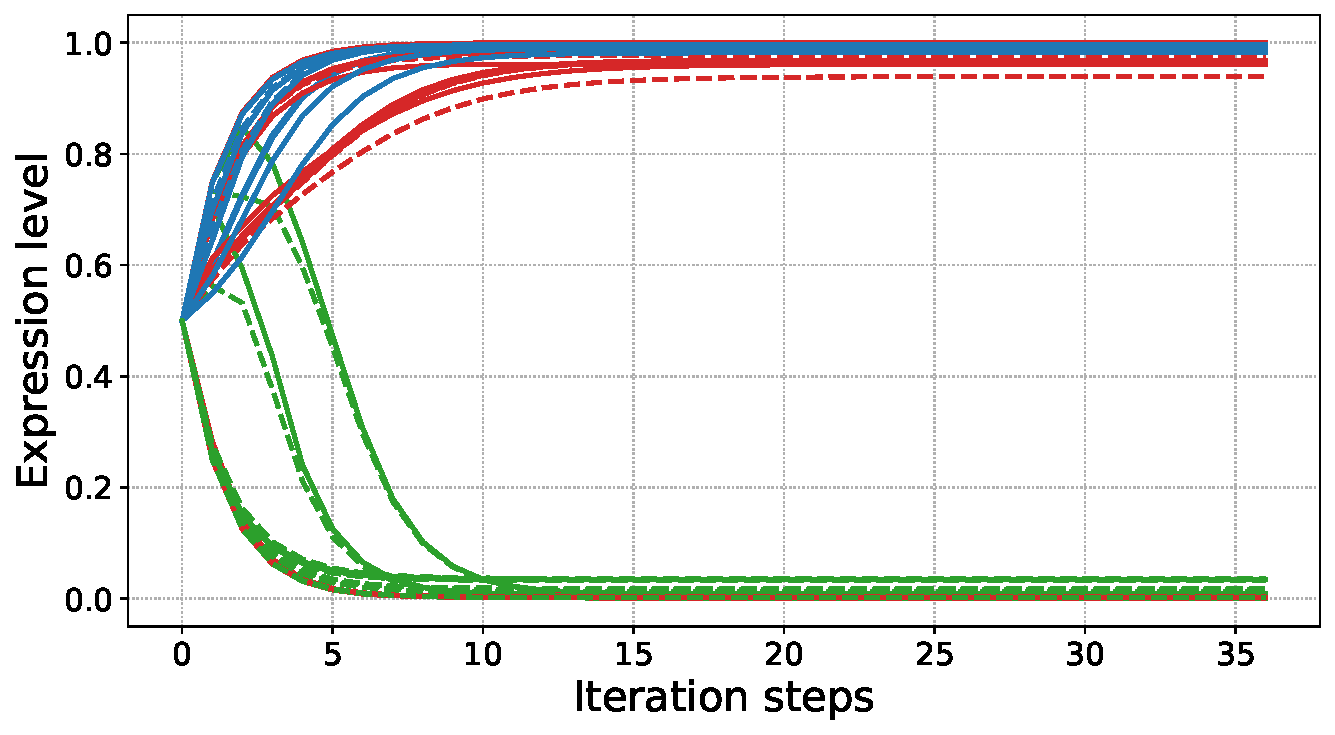
\includegraphics[width=\textwidth]{alife/img/best_rep13_env_A.pdf}
\label{subfig:alife:best_expr_A}
\end{subfigure}
\vspace{-5mm}

\begin{subfigure}[t]{0.42\textwidth}
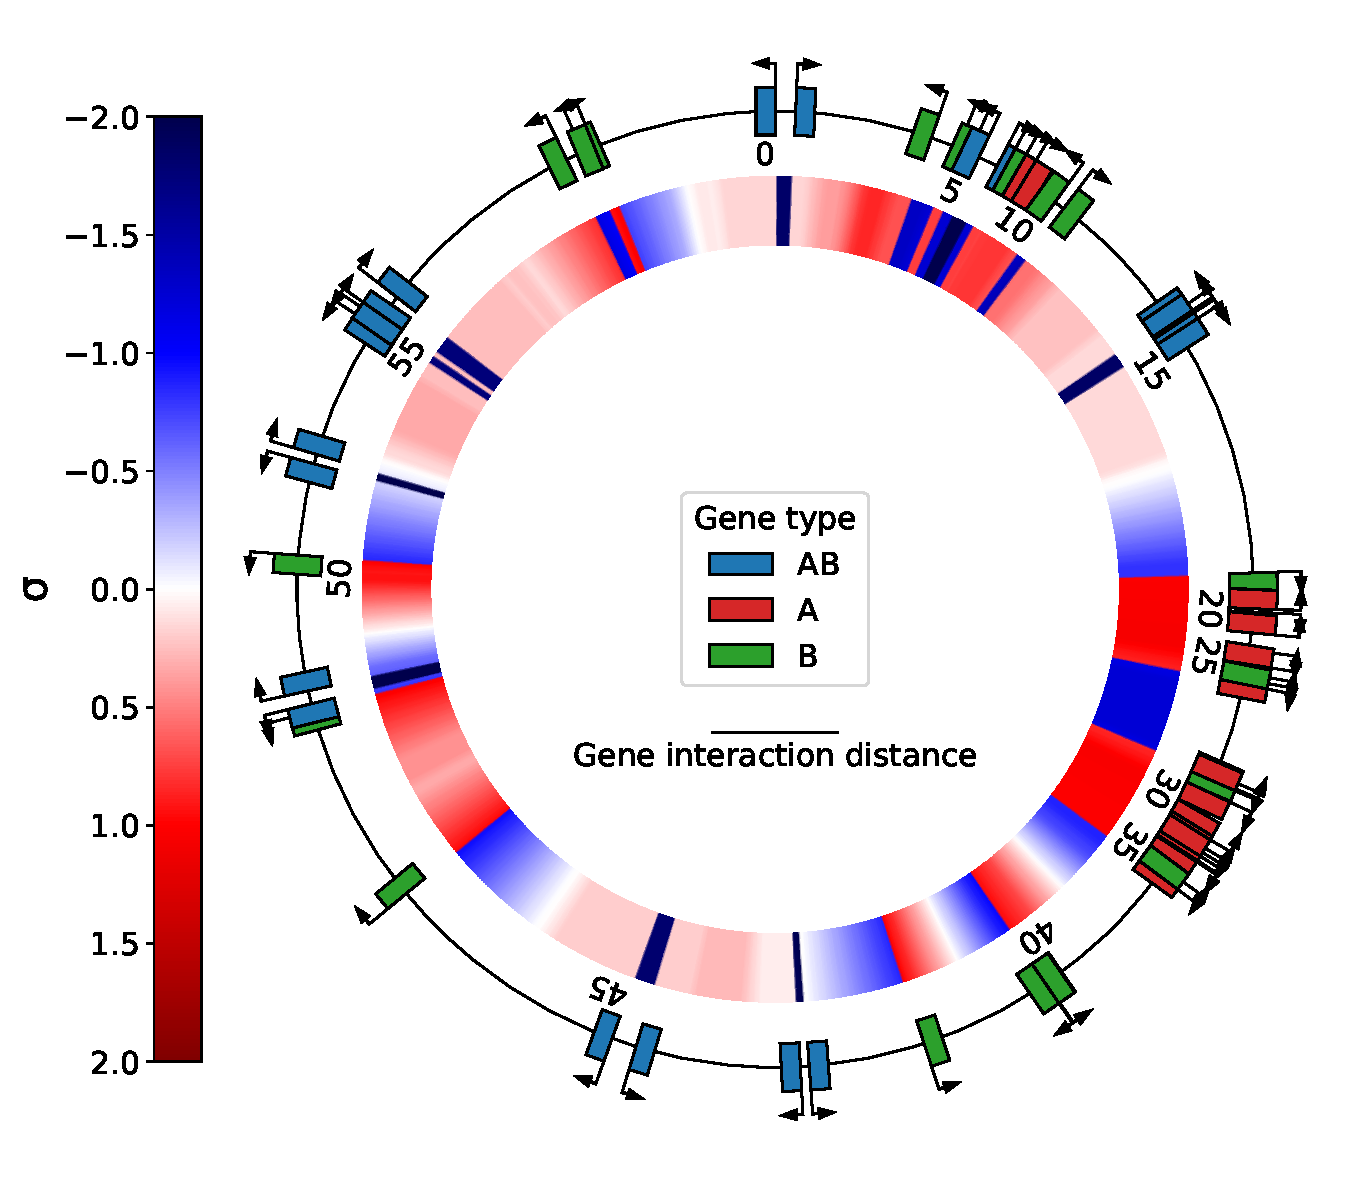
\includegraphics[width=\textwidth]{alife/img/genome_and_tsc_rep13_env_B.pdf}
\label{subfig:alife:best_genome_B}
\end{subfigure}
\begin{subfigure}[t]{0.56\textwidth}
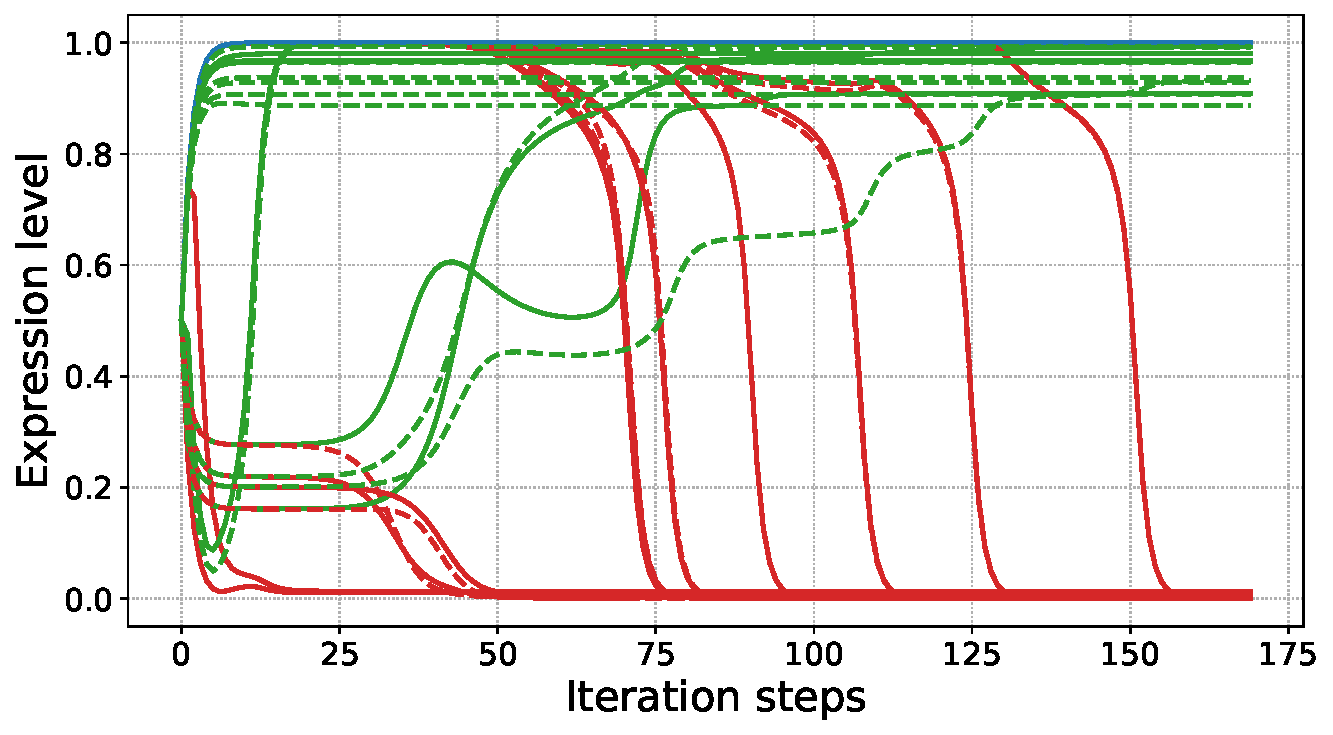
\includegraphics[width=\textwidth]{alife/img/best_rep13_env_B.pdf}
\label{subfig:alife:best_expr_B}
\end{subfigure}
\caption[Best individual at the end of evolution in one of the replicates in the proof-of-concept model, evaluated in both environments]{Local supercoiling along the genome and gene transcription levels of the best individual in replicate 13 after 250,000 generations.
Environment A is on top and environment B at the bottom.
\emph{AB} genes are colored blue, \emph{A} genes colored red, and \emph{B} genes colored green.}
\label{fig:alife:best_indiv}
\end{figure}

Our experimental results show that, in a model of gene transcription that is structured around the transcription"=supercoiling coupling, complex gene interaction networks can in fact evolve.
These gene interaction networks are sensitive to environmental variations, which are mediated in our model by a single parameter: $\sigma_{env}$, the amount of global supercoiling that is due to the environment.

\subsection{Robustness of Gene Network Evolution}
\label{sec:alife:param_explor}

In order to ensure that our results remain experimentally valid over a broad range of parameter values, we ran additional sets of simulations.
We changed respectively the sensitivity of gene promoters to supercoiling changes ($\epsilon$ in equation~\ref{eq:transcr}), the interaction coefficient used in computing the local supercoiling due to the transcription-supercoiling coupling ($c$ in equation~\ref{eq:dsde}), and the strength of the change in supercoiling imposed by the environment ($\sigma_A$ and $\sigma_B$).
We chose sets of logarithmically-spaced values for each parameter, and ran 5 replicates of the evolution experiment for 250,000 generations for each parameter value.
Note that, for extreme parameter values, gene expression levels did in some cases not converge to stable states by the maximum number of computation steps.
In this situation, we chose to retain the gene expression levels at the last step as the phenotype of the affected individuals.

\begin{figure}[H]
\centering
\begin{subfigure}[t]{0.49\textwidth}
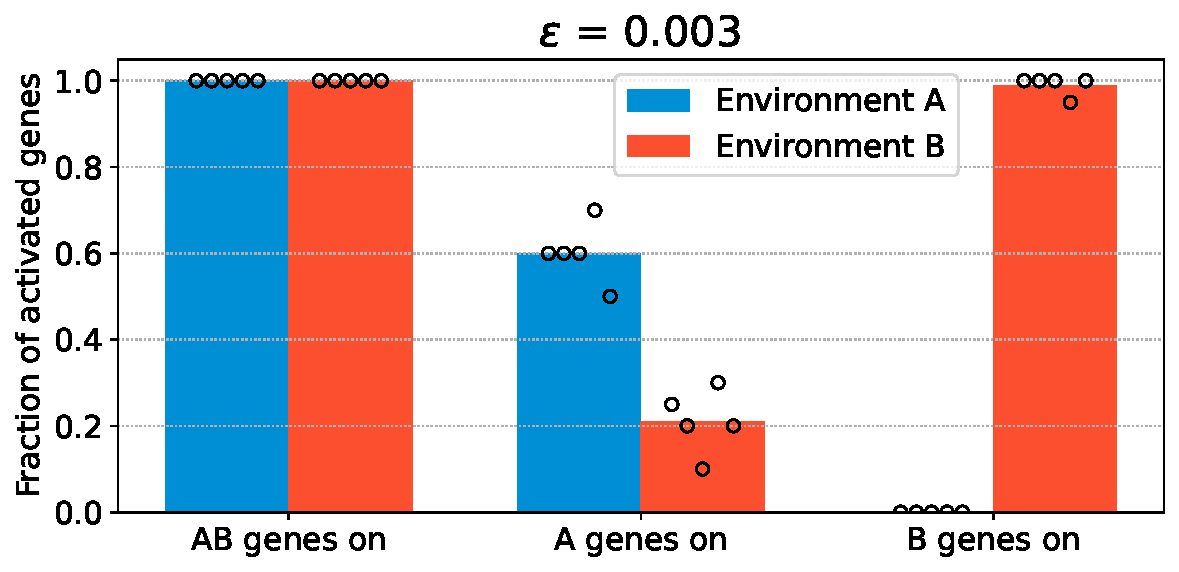
\includegraphics[width=\textwidth]{alife/img/mean_activation_epsilon-0.003.pdf}
\label{subfig:alife:param_epsilon_1}
\end{subfigure}
\begin{subfigure}[t]{0.49\textwidth}
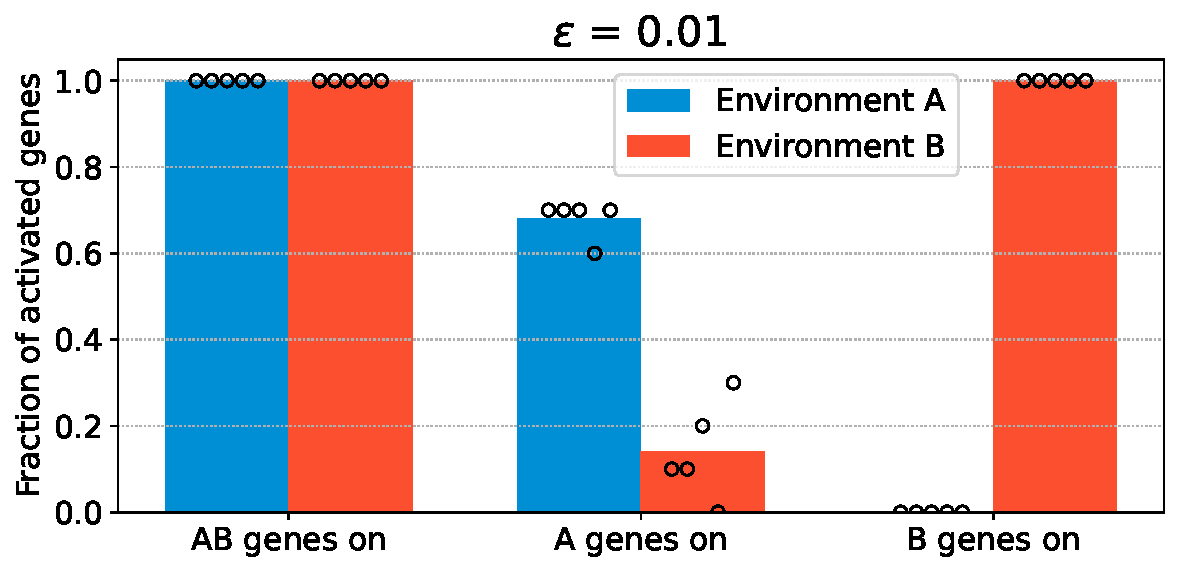
\includegraphics[width=\textwidth]{alife/img/mean_activation_epsilon-0.01.pdf}
\label{subfig:alife:param_epsilon_2}
\end{subfigure}

\begin{subfigure}[t]{0.49\textwidth}
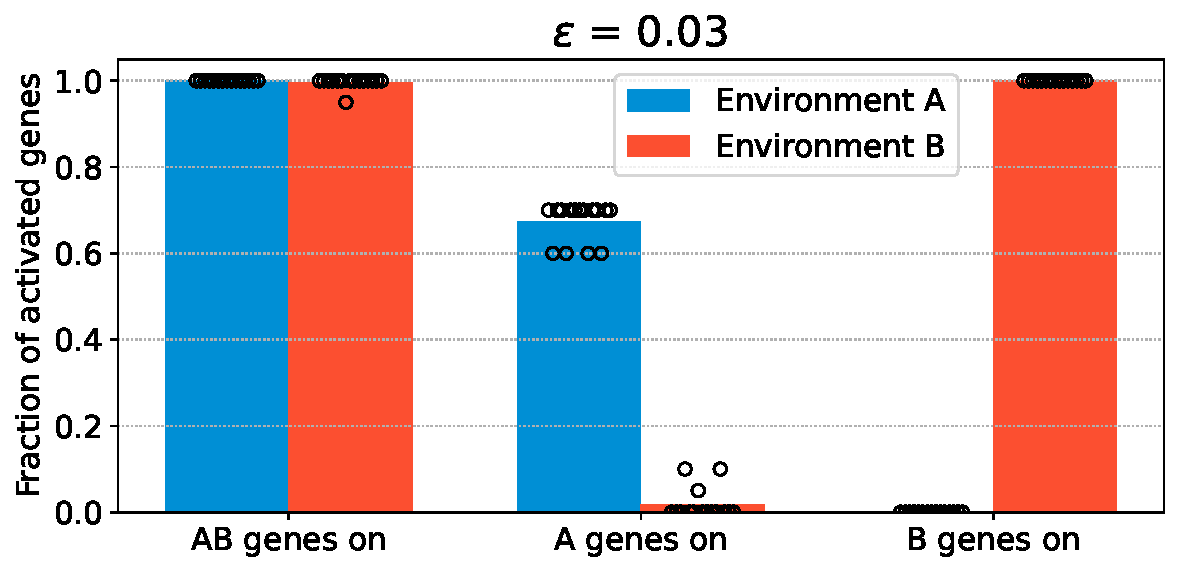
\includegraphics[width=\textwidth]{alife/img/mean_activation_epsilon.pdf}
\label{subfig:alife:param_epsilon_3}
\end{subfigure}
\begin{subfigure}[t]{0.49\textwidth}
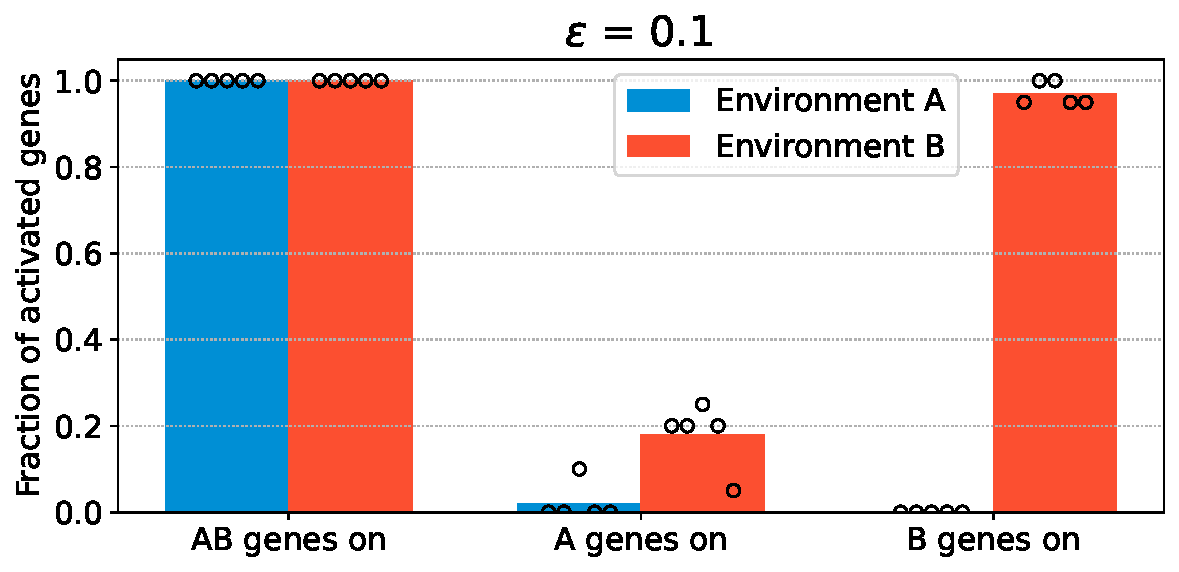
\includegraphics[width=\textwidth]{alife/img/mean_activation_epsilon-0.1.pdf}
\label{subfig:alife:param_epsilon_4}
\end{subfigure}
\caption[Parameter exploration in the proof-of-concept model: varying $\epsilon$]{Average fraction of activated genes in each environment at the end of evolution, for increasing values of $\epsilon$, from top to bottom and left to right.
Every replicate is shown as a dot, and the bottom-left panel ($\epsilon = 0.03$) recalls data from the main run (which has 15 replicates) for comparison.
For all values of $\epsilon$ except $0.1$, the behavior from the main run is qualitatively replicated.}
\label{fig:alife:param_epsilon}
\end{figure}

The results of these additional simulations are presented in figures~\ref{fig:alife:param_epsilon},~\ref{fig:alife:param_c} and~\ref{fig:alife:param_sigma}.
For $\epsilon$, we chose values of $\epsilon = 0.003$, $\epsilon = 0.01$, and $\epsilon = 0.1$, compared to an initial value of $\epsilon = 0.03$, and the results are shown in Figure~\ref{fig:alife:param_epsilon}.
For the values of $\epsilon$ lower than the default (top row), representing a higher sensitivity of promoters to supercoiling, we observe the evolution of differentiated gene expression levels as in the main run (bottom-left panel), whereas for the higher value of $\epsilon$ (bottom-right panel), \emph{A} genes are still not expressed in environment A by the end of evolution.
In this case, promoters are not sensitive enough to the supercoiling variations caused by the transcription-supercoiling coupling, and genes are unable to overcome the highly positive supercoiling of environment A.

\begin{figure}[H]
\centering
\begin{subfigure}[t]{0.49\textwidth}
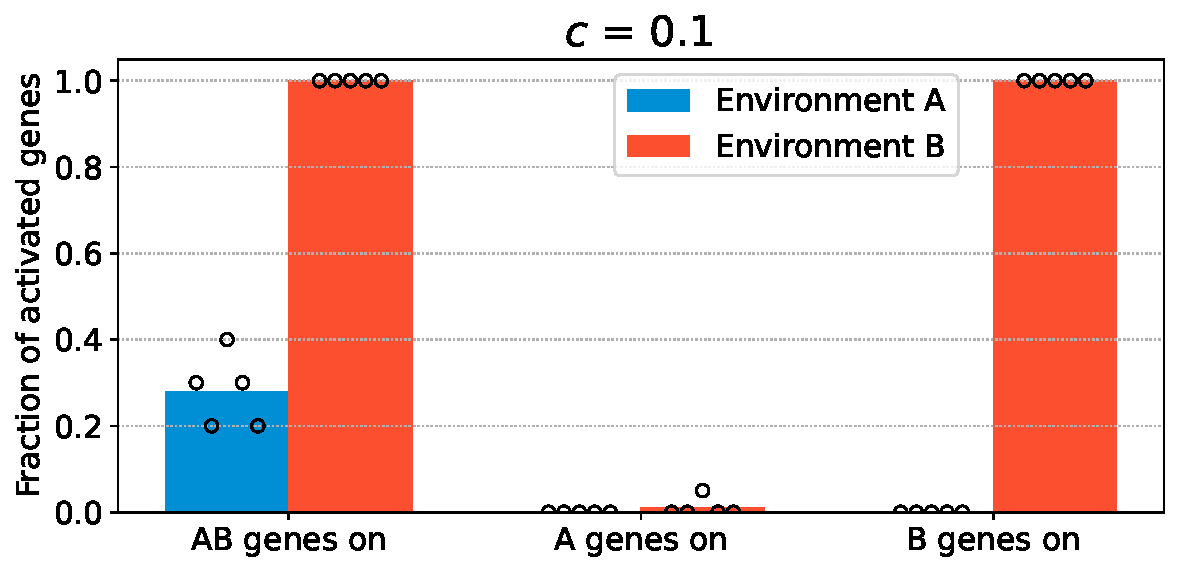
\includegraphics[width=\textwidth]{alife/img/mean_activation_inter-coef-0.1.pdf}
\label{subfig:alife:param_c_1}
\end{subfigure}
\begin{subfigure}[t]{0.49\textwidth}
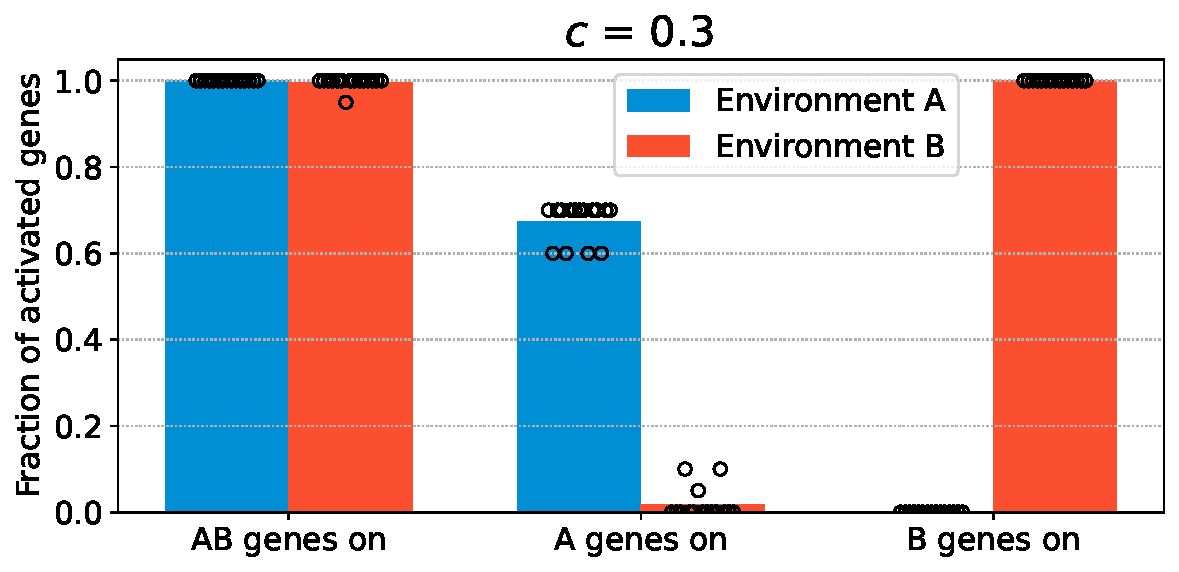
\includegraphics[width=\textwidth]{alife/img/mean_activation_inter_coef.pdf}
\label{subfig:alife:param_c_2}
\end{subfigure}

\begin{subfigure}[t]{0.49\textwidth}
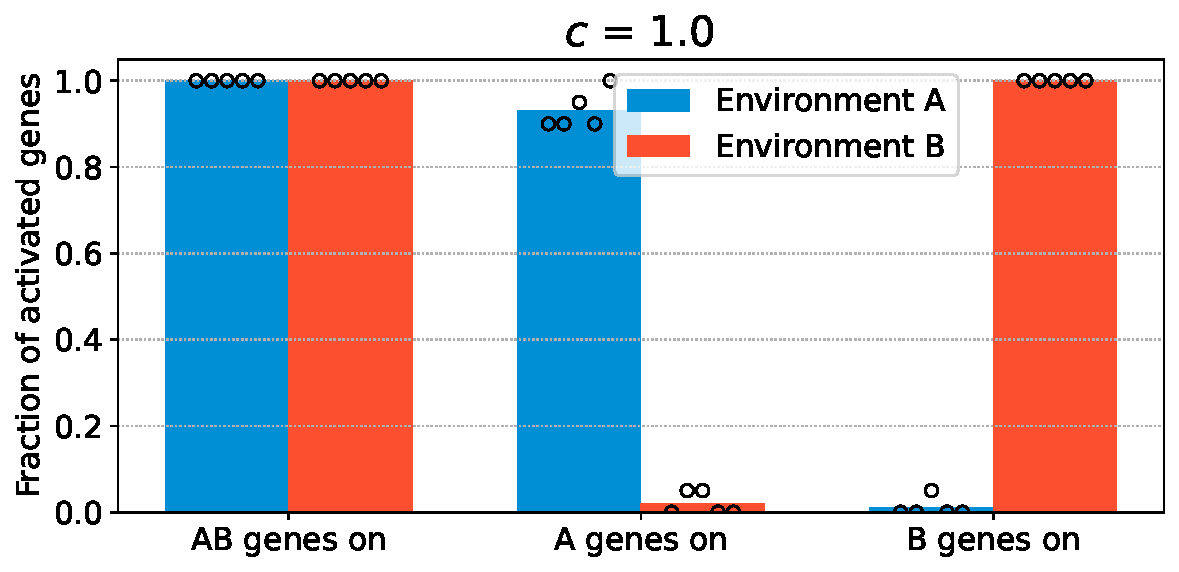
\includegraphics[width=\textwidth]{alife/img/mean_activation_inter-coef-1.0.pdf}
\label{subfig:alife:param_c_3}
\end{subfigure}
\begin{subfigure}[t]{0.49\textwidth}
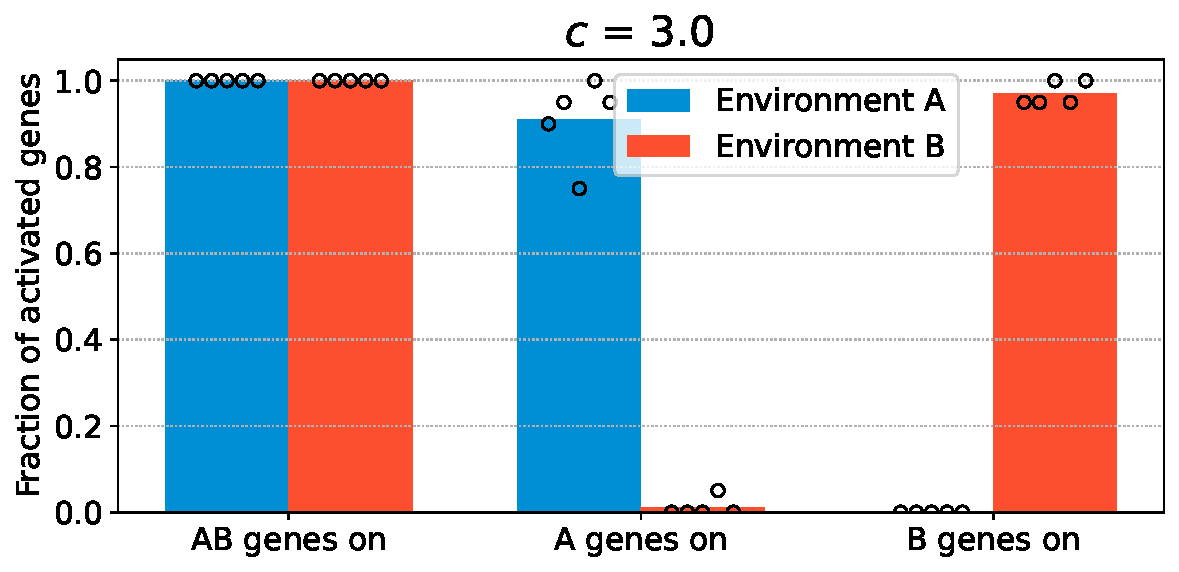
\includegraphics[width=\textwidth]{alife/img/mean_activation_inter-coef-3.0.pdf}
\label{subfig:alife:param_c_4}
\end{subfigure}
\caption[Parameter exploration in the proof-of-concept model: varying $c$]{Average fraction of activated genes in each environment at the end of evolution, for increasing values of $c$, from top to bottom and left to right.
Every replicate is shown as a dot, and the top-right panel ($c = 0.3$) recalls data from the main run for comparison.
For all values of $c$ except $0.1$, the behavior from the main run is qualitatively replicated.}
\label{fig:alife:param_c}
\end{figure}

For $c$, we chose values of $c = 0.1$, $c = 1.0$, and $c = 3.0$, for an initial value of $c = 0.3$, and the results are shown in Figure~\ref{fig:alife:param_c}.
Similarly to $\epsilon$, when $c$ is too low (top-left panel), genes do not interact strongly enough for a differentiated phenotype to evolve as a function of the environment, whereas higher values of $c$ (bottom row) show the same evolutionary behavior as the main run (top-right panel).

\begin{figure}[H]
\begin{subfigure}[t]{0.49\textwidth}
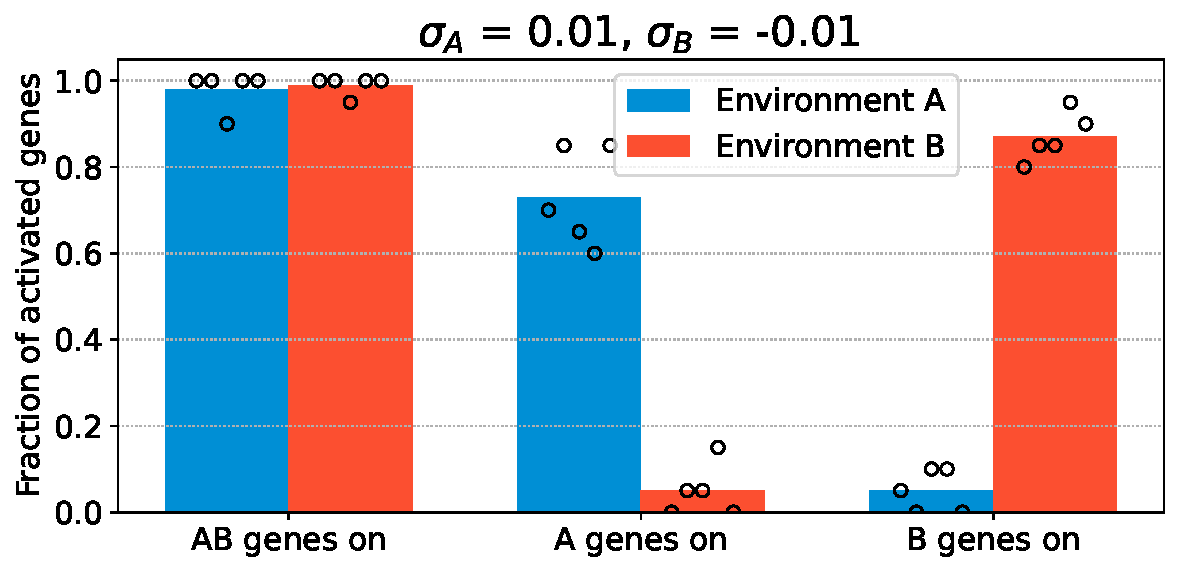
\includegraphics[width=\textwidth]{alife/img/mean_activation_sigma-0.01.pdf}
\label{subfig:alife:param_sigma_1}
\end{subfigure}
\begin{subfigure}[t]{0.49\textwidth}
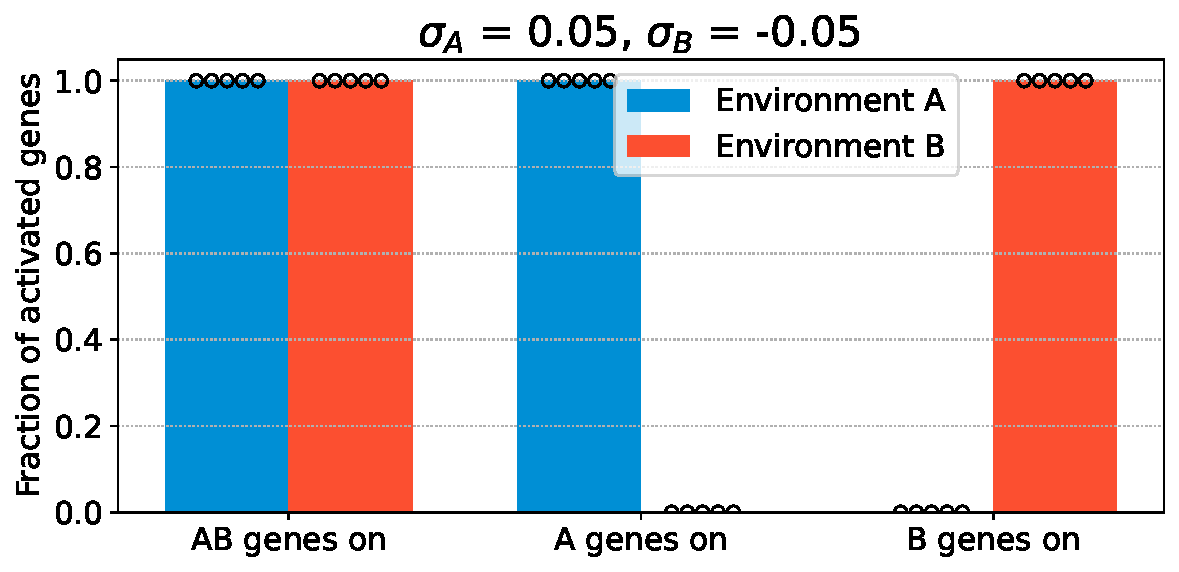
\includegraphics[width=\textwidth]{alife/img/mean_activation_sigma-0.05.pdf}
\label{subfig:alife:param_sigma_2}
\end{subfigure}

\begin{subfigure}[t]{0.49\textwidth}
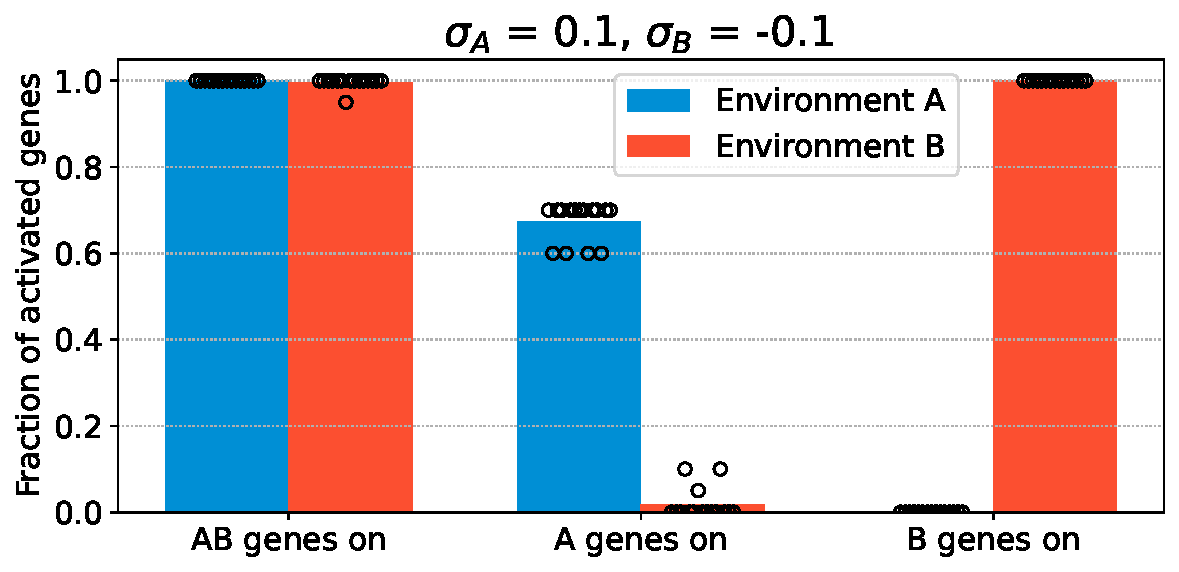
\includegraphics[width=\textwidth]{alife/img/mean_activation_sigma.pdf}
\label{subfig:alife:param_sigma_3}
\end{subfigure}
\begin{subfigure}[t]{0.49\textwidth}
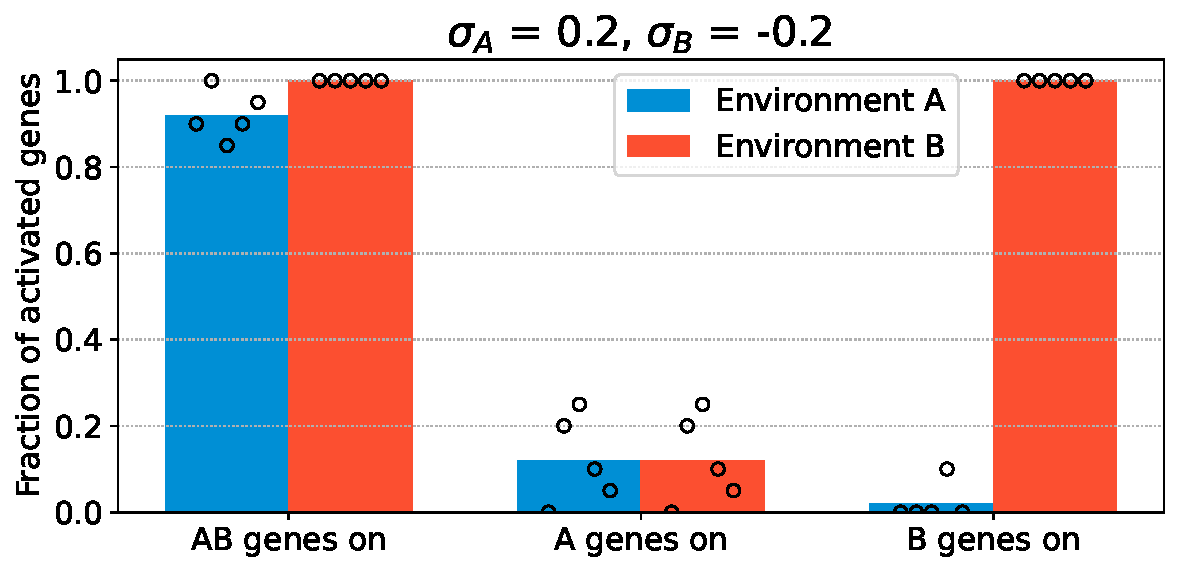
\includegraphics[width=\textwidth]{alife/img/mean_activation_sigma-0.2.pdf}
\label{subfig:alife:param_sigma_4}
\end{subfigure}
\caption[Parameter exploration in the proof-of-concept model: varying $\sigma_A$ and $\sigma_B$]{Average fraction of activated genes in each environment at the end of evolution, for more and more distinct environments $\sigma_A$ and $\sigma_B$, from top to bottom and left to right.
Every replicate is shown as a dot, and the bottom-left panel ($\sigma_A = 0.1$, $\sigma_B = -0.1$) recalls data from the main run for comparison.
For all values except $\sigma_A = 0.2$ and $\sigma_B = -0.2$, the behavior from the main run is qualitatively replicated.}
\label{fig:alife:param_sigma}
\end{figure}

Finally, we also investigate different amplitudes in the difference in supercoiling level between the two environments, by choosing values of $\sigma_A = 0.01$, $\sigma_A = 0.05$ and $\sigma_A = 0.2$, and $\sigma_B = -\sigma_A$ respectively in each case (for an initial value of $\sigma_A = 0.1$ and $\sigma_B = -0.1$).
We observe that, when $\sigma_A = 0.2$ (bottom-right panel), the environmental supercoiling constraint is too high and \emph{A} genes are not activated in environment A by the end of the runs.
However, for environments closer to each other than the default (top row), evolution is able to leverage the differences in supercoiling between these environments to evolve differentiated phenotypes, as in the main run (bottom-left panel), showing that our model remains sensitive to small changes in environmental supercoiling.

To conclude, in our model, the gene interaction network is therefore able to respond to different environments and can evolve an efficient regulation of gene expression under a broad range of parameter values, reinforcing the hypothesis that a supercoiling-mediated coupling between gene expression levels could indeed play a functional role in biological organisms.

\section{Discussion and Perspectives}

DNA supercoiling plays a fundamental role in the regulation of gene transcription in bacteria, and an important part of this role could be mediated by the local variations in supercoiling that are caused by the transcription-supercoiling coupling.
While the influence of the global supercoiling level on gene transcription~\citep{lal2016, ma2016,dorman2016, martisb.2019}, the evolutionary importance of supercoiling regulation~\citep{crozat2005,crozat2010, duprey2021} and the mechanistic details of the transcription-supercoiling coupling~\citep{meyer2014, elhoudaigui2019} have all already been studied, no existing work did to our knowledge tackle the question of the possible role of the transcription-supercoiling coupling both at the whole-genome scale and on an evolutionary time scale.

In this work, we have developed a genome-wide model of the influence of DNA supercoiling on gene transcription, incorporating both the global influence of the environment and the local variations in the supercoiling level that are due to the transcription-supercoiling coupling.
We have shown that, in our model, complex interactions implicating several genes emerge from the coupling between supercoiling and transcription.
Indeed, \emph{A} genes display an activation pattern that would not be obtainable without the network of interactions that results from the coupling.
Thanks to this network, \emph{A} genes are activated in an environment where isolated genes would be inhibited, and inhibited in an environment where isolated genes would be activated.
The transcription-supercoiling coupling therefore enables the selective activation or inhibition of specific sets of genes, providing a non-monotonic response to environmental variations through changes in the level of DNA supercoiling.
Furthermore, we have shown, using an \emph{in silico} experimental evolution approach, that natural selection can leverage this biophysical mechanism to selectively turn on or off several pools of genes, using only the very simple mutation operator of genomic inversions, that affect the relative positions and orientations of genes on the genome but do not change genome length or basal gene transcription rates, and that this behavior is able to evolve under a wide range of parameter values.
This response of gene transcription levels to DNA supercoiling reflects a phenomenon which has been observed \emph{in vivo} in the expression of pathogenicity-related genes in specific environments, such as the normally lethal inside of the macrophage for the mammalian pathogen \emph{S. enterica}~\citep{cameron2013}, or plant tissue for \emph{D. dadantii}~\citep{herault2014}.

Our model voluntarily stays very simple, only incorporating the most important feature of the transcription-supercoiling coupling, which is the non-linear interaction between the expression levels of neighboring genes.
This simplicity therefore hints at the possible pervasiveness of this regulation mechanism throughout the prokaryotic realm.
Nonetheless, in order to go further and represent more accurately the diversity of gene behaviors found in real life, several more dimensions could be integrated to the model.
At present, the target for genes in our model is bistability, meaning that genes should end up fully activated or fully inhibited.
A more biologically plausible approach would be to relax this restriction and give genes arbitrary expression targets, in order to determine to which extent the transcription-supercoiling coupling is able to finely regulate gene expression.
Furthermore, unlike in our model (in which all genes have the same response curve to DNA supercoiling), the genes of biological organisms can show different responses to the supercoiling level.
These differences are partly caused by the GC content at the gene promoter~\citep{forquet2021}, and some genes can even respond in the opposite direction to DNA relaxation, that is to say be activated rather than inhibited by less negatively supercoiled DNA.
This behavior is for instance present in the \emph{gyrA} and \emph{gyrB} genes that encode the gyrase subunits in \emph{E. coli}~\citep{peter2004}.
Moreover, while our model studies its role in an abstract transcription model, supercoiling intervenes during different parts of the initiation and termination of transcription, as well as in in transcript elongation~\citep{martisb.2019}.
Incorporating such precise mechanistic processes into our model could give more accurate information on the link between the position of genes on the genome and their transcription rate.
Similarly, increasing the number of genes of individuals in our model to match bacterial gene numbers might provide more fine-grained results, but is computationally intractable in the current implementation of the model.
Furthermore, investigating the behaviors of individuals when they are placed successively in different environments, rather than evaluated separately in each environment, would also bring more information on the plasticity of the network of gene interaction levels that emerges from the transcription-supercoiling coupling.
Finally, another valuable approach in order to bring this model closer to biology would be to incorporate it into a larger existing framework, such as the Aevol \emph{in silico} experimental evolution platform~\citep{rutten2019}, which models the bacterial genome in much more detail, in order to leverage the power of a well-understood digital organism model.

\chapter{PLOS CB Paper}
\label{chap:ploscb}

\section{Background}

DNA, the material basis of genetic information, is a flexible polymer comprising two strands of nucleotides that coil around each other, at a rate of 10.5 base pairs per turn.
When subjected to torsional stress, DNA can either writhe and form 3-dimensional loops, or twist around itself more or less tightly than in its relaxed state~\citep{travers2005}; both forms are referred to as DNA supercoiling, which is measured as the relative density of supercoils $\sigma$ compared to relaxed DNA.
DNA is positively supercoiled ($\sigma > 0$) when it is overwound, and negatively supercoiled ($\sigma < 0$) when it is underwound.
In bacteria, DNA is normally maintained in a moderately negatively supercoiled state, with a reference value of $\sigma=-0.06$ in \emph{Escherichia coli}~\citep{travers2005}.
DNA supercoiling plays an important role in the regulation of gene expression in bacteria~\citep{martisb.2019}, as it is highly dynamic, and varies in both space along the chromosome and time during the cell lifecycle~\citep{krogh2018}, and as the level of supercoiling at the promoter of a gene modulates the expression of that gene~\citep{forquet2021}.
Furthermore, gene transcription itself locally impacts the level of DNA supercoiling, resulting in an interplay between the supercoiling and transcription of neighboring genes~\citep{meyer2014}, which hints at a possible role for this coupling as an evolutionary force shaping genome organization~\citep{junier2016}.

\subsection{The Dynamic Nature of DNA Supercoiling}

The level of DNA supercoiling in bacteria is controlled by topoisomerases, enzymes that alter DNA supercoiling by cutting and rotating the DNA strands~\citep{duprey2021}; the two main topoisomerases being gyrase, which dissipates positive supercoiling by introducing negative supercoils at an ATP-dependent rate, and topoisomerase I, which oppositely relaxes negative supercoiling~\citep{martisb.2019}.
Many other processes however influence the level of DNA supercoiling.
According to the twin-domain of supercoiling~\citep{liu1987}, the transcription of a gene by RNA polymerase generates a buildup of positive supercoiling upstream of the gene, and negative supercoiling downstream of the gene, through the rotational drag that hampers the rotation of the polymerase around DNA.
At a larger scale, while the intrinsic flexibility of the DNA polymer would allow supercoils to propagate freely along its length, many nucleoid-associated proteins such as FIS, H-NS or HU bind to bacterial DNA (in addition to RNA polymerases), and create topological barriers that instead block the diffusion of supercoiling~\citep{travers2005}.
In bacteria, the level of DNA supercoiling can furthermore be affected by numerous environmental challenges.
Salt shock transiently increases negative DNA supercoiling in \emph{E. coli}~\citep{hsieh1991}; the acidic intracellular environment relaxes DNA in the facultative pathogen \emph{Salmonella enterica} var. Typhimurium~\citep{marshall2000}; and higher temperatures relax DNA in the plant pathogen \emph{Dickeya dadantii}~\citep{herault2014}.
These constraints overall result in a very dynamic DNA ``supercoiling landscape'' in \emph{E. coli}~\citep{visser2022}, with a supercoiling level that varies in both time during the bacterial lifecycle and space along the chromosome.
%, but increases negative supercoiling in the human pathogen \emph{Shigella flexneri}~\citep{tobe1995}. % Note: at the promoter of _virB_ yes, but not genome-wide

\subsection{DNA Supercoiling and Gene Regulation}

Many bacteria leverage the regulating effect of DNA supercoiling on gene transcription by modulating their DNA supercoiling level.
In several bacteria such as \emph{E. coli}, \emph{S. enterica}, or \emph{D. dadantii}, between 5\% and 15\% of genes were found to be sensitive to relaxation or hypercoiling of chromosomal DNA, with genes being up-regulated or down-regulated in each condition~\citep{peter2004, ferrandiz2010, webber2013, pineau2022a}.
DNA supercoiling might in particular be an especially important regulator of gene activity in bacteria with reduced genomes, such as the obligate aphid endosymbiotic bacterium \emph{Buchnera aphidicola}, which is nearly devoid of transcription factors~\citep{brinza2013}.

Moreover, selection can act on the level of DNA supercoiling in order to modulate the regulation of gene expression.
In 10 of the 12 populations in the Long-Term Evolution Experiment (LTEE), an increase in fitness was linked to mutations in the \emph{topA} and \emph{fis} genes, which participate in the regulation of the supercoiling level~\citep{crozat2010}.
When inserted into the ancestral strain, these mutations increased the level of negative supercoiling as well as the bacterial growth rate~\citep{crozat2005}, demonstrating that the level of DNA supercoiling can evolve as part of a regulatory response to new environments.

Finally, the regulation of gene expression by DNA supercoiling could be a force that participates in shaping the evolution of bacterial genomes themselves.
Indeed, supercoiling-sensitive genes tend to group in up or down-regulated clusters in \emph{E. coli}~\citep{peter2004}, \emph{S. enterica}~\citep{webber2013} and \emph{S. pneumoniae}~\citep{ferrandiz2010}, suggesting the possibility of an adaptive role in the co-localization of these clusters.
Indeed, synteny segments, or clusters of neighboring genes that show correlated expression patterns, are evolutionarily conserved across \emph{E. coli} and the distantly related \emph{Bacillus subtilis}~\citep{junier2016}, strengthening the hypothesis that these domains could play an important role in the regulation of bacterial gene expression.

\subsection{The Transcription-Supercoiling Coupling}

As we saw before, the process of transcribing a given gene generates an accumulation of positive supercoiling downstream of that gene, and of negative supercoiling upstream of that gene~\citep{liu1987}.
If a second gene is located closely enough to this first gene, the change in supercoiling at the promoter of the second gene will impact its transcription rate, as negative supercoiling usually facilitates promoter opening, and hence gene transcription~\citep{forquet2021}.
In turn, the second gene will also generate a change in supercoiling that affects the first gene, resulting in an interaction between the transcription levels of these two genes.
Depending on the relative orientation of these genes, several types of interactions are therefore possible: divergent genes reinforce their respective transcription level in a positive feedback loop, convergent genes inhibit the transcription of one another, and for tandem genes, the downstream gene up-regulates the upstream gene, while the upstream gene down-regulates the downstream gene.

This effect, which has been called the transcription-supercoiling coupling~\citep{meyer2014,sobetzko2016,elhoudaigui2019}, has been documented in several bacterial genetic systems.
In \emph{S. flexneri}, the \emph{virB} promoter is normally only active at high temperature, but can be activated at low temperature by the insertion of a phage promoter in divergent orientation~\citep{tobe1995}.
Similarly, the expression of the \emph{leu-500} promoter in \emph{S. enterica} can be increased or decreased by the insertion of upstream transcriptionally active promoters, depending on their orientation relative to \emph{leu-500}~\citep{elhanafi2000}.
The magnitude of this effect has also been explored in a synthetic construct that uses the inducible \emph{ilvY} and \emph{ilvC} \emph{E. coli} promoters, inserted on a plasmid in divergent orientations.
In this system, a decrease in the activity of \emph{ilvY} is associated with a decrease in \emph{ilvC} activity, and an increase in \emph{ilvY} activity with an increase in \emph{ilvC} activity as well~\citep{rhee1999}.

There are, however, hints that the biological relevance of the transcription-supercoiling coupling might not be confined to a few specific cases.
Indeed, in \emph{E. coli}, the typical size of topological domains, inside which the supercoiling generated by gene transcription can propagate, is usually around 10kb~\citep{postow2004}, and could reach up to 25kb~\citep{visser2022} in each direction.
As the average size of \emph{E. coli} genes is 1kb, and the average intergenic distance about 120bp~\citep{blattner1997}, this means that any single topological domain encompasses several genes that can potentially interact via the transcription-supercoiling coupling.
A statistical analysis of the relative position of neighboring genes on the \emph{E. coli} chromosome furthermore shows that genes that are up-regulated by negative supercoiling have more neighbors in divergent orientations, while genes that are down-regulated by negative supercoiling have more neighbors in converging orientations~\citep{sobetzko2016}, suggesting that the transcription-supercoiling coupling plays a role in regulating the activity of these genes.

\paragraph{}
In this article, we present a two-level individual-based model of gene expression at the whole-genome scale, in which gene transcription is regulated solely by DNA supercoiling, and in which populations of individuals evolve towards environment-specific gene expression targets through genomic rearrangements only.
Rather than attempting to give quantitative predictions of the  effect of the transcription-supercoiling coupling on the expression levels of genes in a given, static genetic system, our model aims at exploring the range of genomic organizations that can be generated by selection in order to regulate gene expression levels in different environments through the transcription-supercoiling coupling.
Using this model, we observe the emergence of complex environment-driven patterns of gene expression, and characterize the spatial organization of genes along the genome that underlie these patterns.
We first show that genes are locally organized in convergent or divergent pairs that leverage the transcription-supercoiling coupling to activate or inhibit one another.
Then, we show that this local organization is not entirely sufficient to fully account for the complex gene expression patterns that we observe, but that gene inhibition requires the interaction of a large number of genes.
Finally, we show that, in our model, genes form a dense genome-wide regulatory network, providing insight into the organization of bacterial genomes.


\section{An Evolutionary Model of the Transcription-Supercoiling Coupling}
\label{sec:ploscb:model}

\subsection{Individual-Level Model}
\label{sec:ploscb:indiv_model}

We define the genotype of an individual in our model as a single circular chromosome that is representative of a bacterial chromosome.
The chromosome consists in a fixed number of protein-coding genes, which are separated by non-coding intergenic segments of varying sizes, and has a basal supercoiling level $\sigma_{basal}$.
Each gene on the chromosome is characterized by its starting position (genes cannot overlap in our model), its orientation (on the forward strand or on the reverse strand), its length, and its basal expression level.
We define an environment by the shift $\delta\sigma_{env}$ that it imposes to the supercoiling level of the chromosome.
We then define the phenotype of an individual in a given environment as the gene expression levels that are solution of the system given by the interaction of its genes through the transcription-supercoiling coupling (described below), on a chromosome with a background supercoiling level of $\sigma_{basal} + \delta\sigma_{env}$.

\begin{figure}[H]
  \centering
  \begin{subfigure}[t]{0.44\textwidth}
    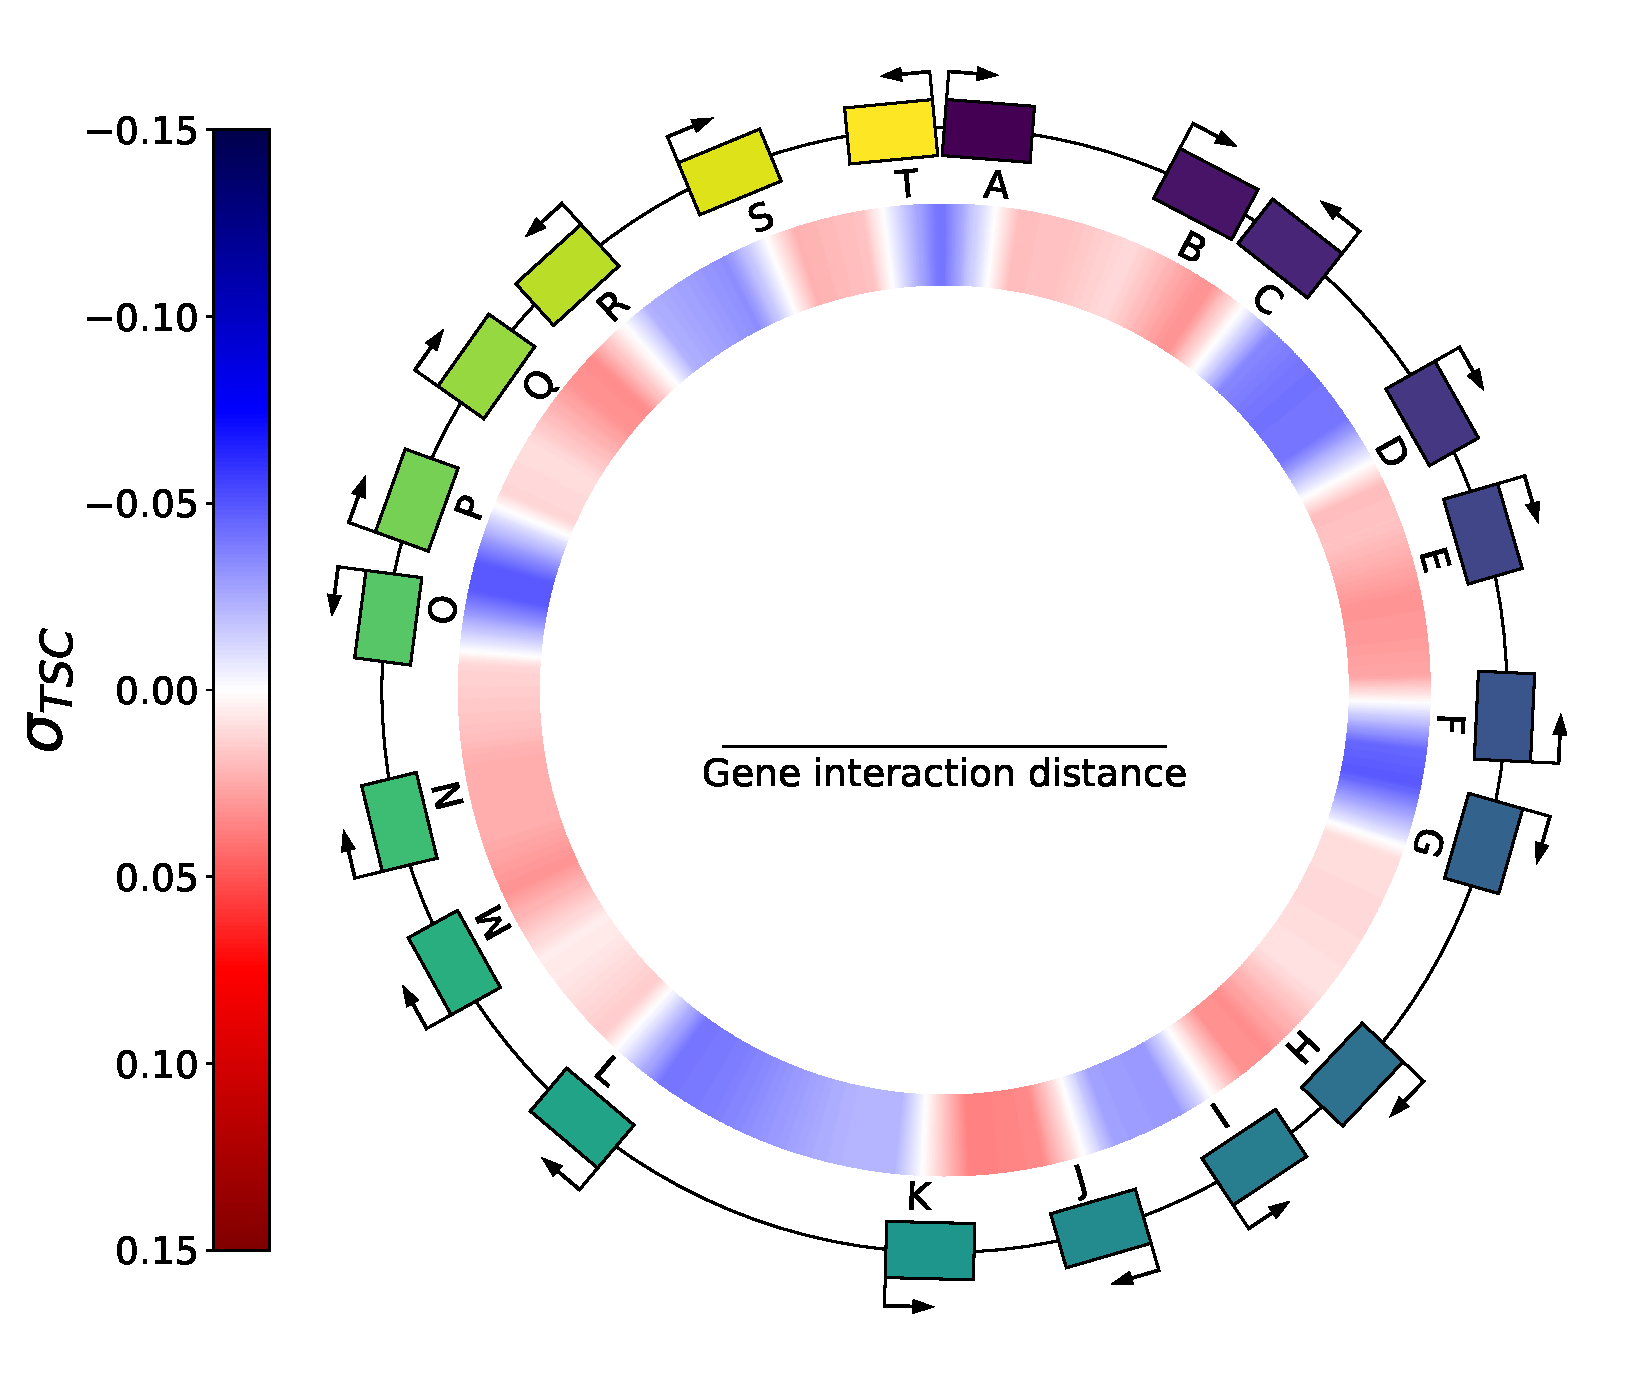
\includegraphics[width=\textwidth]{ploscb/img/random_genome_and_tsc.pdf}
    \label{subfig:ploscb:random_genome}
  \end{subfigure}
  \begin{subfigure}[t]{0.55\textwidth}
    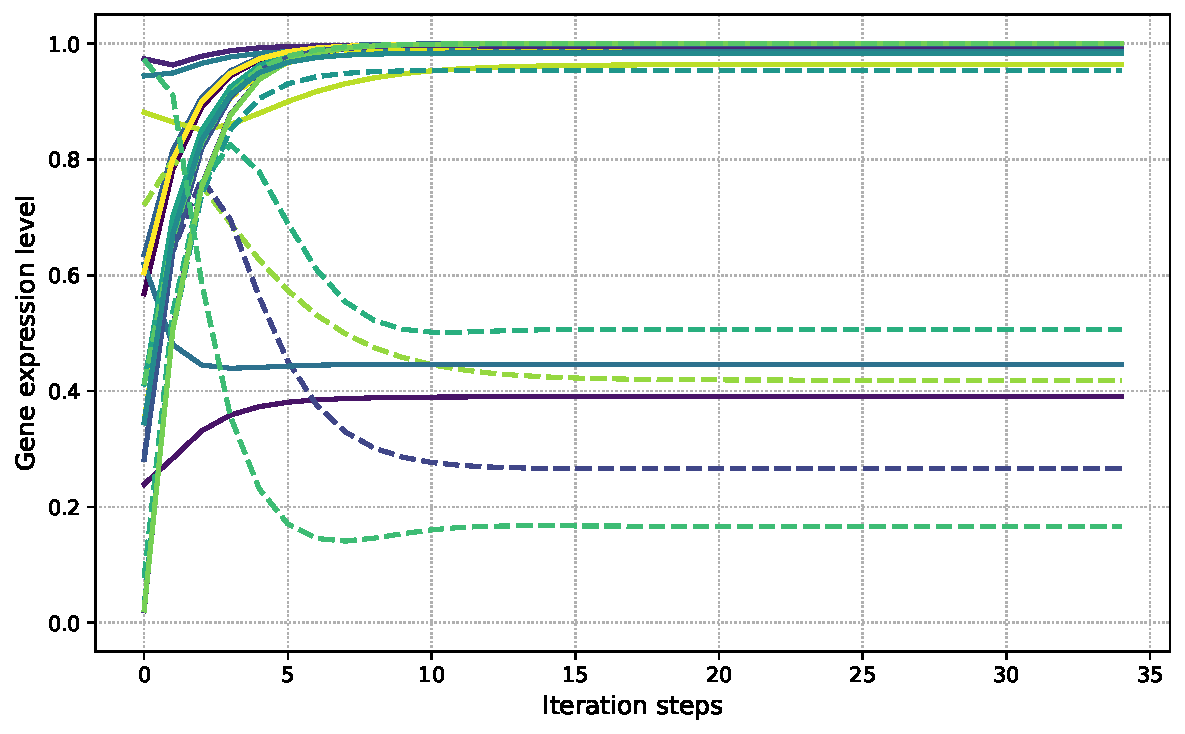
\includegraphics[width=\textwidth]{ploscb/img/random_gene_expr.pdf}
    \label{subfig:ploscb:random_expr}
  \end{subfigure}
  \caption[Example individual in the advanced model, evaluated in both environments]{Left: genome (outer ring) and level of supercoiling generated by transcription ($\sigma_{TSC}$, inner ring) of an example genome with 20 genes placed at random positions and orientations and colored by position, with a gene length and average intergenic distance of 1 kb each, and a basal supercoiling level of $\sigma_{basal} = -0.066$.
  The individual is evaluated in an environment in which $\delta\sigma_{env} = 0$.
  Right: evolution of the expression level of each gene of the individual during the computation of the solution to the system given by equations~\ref{eq:sigma},~\ref{eq:prom_energy}, and~\ref{eq:gene_activity}, starting from random initial values.
  Solid lines represent genes on the forward strand, dashed lines genes on the reverse strand, and gene colors are the same as on the genome.}
  \label{fig:ploscb:random_indiv}
\end{figure}

The genome of an example individual with 20 genes and a basal supercoiling $\sigma_{basal} = -0.066$ is shown on the left-hand side of Figure~\ref{fig:ploscb:random_indiv}.
Inside the genome is the resulting local level of DNA supercoiling when this individual is evaluated in an environment with a supercoiling shift of $\delta\sigma_{env}~=~0$.
As expected given the twin-domain model of supercoiling, we can observe a buildup in negative supercoiling (blue) between genes in divergent orientations, such as genes C and D or F and G, and a buildup in positive supercoiling (red) between genes in convergent orientations, such as genes J and K or Q and R.
The right-hand side panel of Figure~\ref{fig:ploscb:random_indiv} shows the computation of the stable state of gene expression levels for this individual.
Note that, in this model and throughout this article, we conflate
gene transcription rates with mRNA concentrations, as we assume that mRNAs degrade at a constant rate, and as transcription rates in our model are only affected by the effect of supercoiling on transcription.
We furthermore conflate transcription rates with expression levels, as we again assume proteins to be translated at a rate proportional to the associated mRNA concentrations and to degrade at a constant rate.

\paragraph{Effect of Transcription on Supercoiling}
For an individual with a genome containing $n$ genes, each expressed at a level $e_i$, we model the influence of the transcription of each gene on the level of supercoiling at the promoter of every other gene in the form of an $n$-by-$n$ interaction matrix.
The coefficient $\frac{\partial\sigma_i}{\partial e_j}$ at indices $(i, j)$ in this matrix represents the variation in DNA supercoiling at the promoter of gene $i$ due to the transcription of gene $j$.
The value of this coefficient is given by the following formula:

\begin{equation}
  \frac{\partial\sigma_{i}}{\partial e_j} = \eta \cdot c \cdot \max(1-\frac{d(i, j)}{d_{max}}, 0)
  \label{eq:dsigmade}
\end{equation}

$\eta$ represents the sign of the interaction, which depends on the position and orientation of gene $j$ relative to gene $i$, according to the twin-domain model.
If gene $j$ is upstream of gene $i$, and if it is on the same strand as (or points towards) gene $i$, then its transcription generates a buildup in positive supercoiling at gene $i$ ($\eta = 1$).
Conversely, if gene $j$ is upstream of gene $i$ but on the other strand than (or points away from) gene $i$, it generates a buildup in negative supercoiling at gene $i$ ($\eta = -1$).
If gene $j$ is instead located downstream of gene $i$, the sign of the interaction in each case is switched: $\eta = 1$ if the genes are on the same strand, and $\eta = -1$ otherwise.

We then apply a scaling coefficient $c$, which represents the intensity to which the transcription-generated torsion of DNA affects the local level of supercoiling.
Finally, the strength of the interaction decreases linearly with the distance $d(i, j)$ between the promoter of gene $i$, which is the position where the local level of supercoiling affects the probability that an RNA polymerase binds to the DNA and starts transcribing gene $i$, and the middle of gene $j$, which is the average location of the RNA polymerases that transcribe gene $j$, assuming that DNA is transcribed at a constant speed.
When this distance reaches a threshold of $d_{max}$, the two genes are considered to be too far away to interact and the effect vanishes.

\paragraph{Effect of Supercoiling on Transcription}
In order to compute the transcription level of a given gene, we first compute the opening free energy of its promoter, which depends on the local supercoiling level, following a sigmoidal curve that increases with negative supercoiling until a saturation threshold is reached~\citep{forquet2021}.
In order to model this effect, we adapted the equations and parameter values presented in~\cite{elhoudaigui2019}, which are based on the \emph{in vitro} analysis of the transcription of model bacterial promoters.
We first compute the local level of supercoiling $\sigma_i$ at the promoter of gene $i$, which is the sum of the background supercoiling level $\sigma_{basal} + \delta\sigma_{env}$ (which is constant along the genome for any given individual), and of the local variation in supercoiling caused by the transcription of every other gene (represented in Figure~\ref{fig:ploscb:random_indiv} as $\sigma_{TSC}$):

\begin{equation}
  \sigma_i = \sigma_{basal} + \delta\sigma_{env} + \sum_{j=1}^n\frac{\partial\sigma_{i}}{\partial e_j}e_j
  \label{eq:sigma}
\end{equation}

We compute the expression level of the gene using a thermodynamic model of transcription.
First, we compute the opening free energy $U_i$ of the promoter of gene $i$, which depends on $\sigma_i$, the level of supercoiling at the promoter and on $\sigma_0$, the level of supercoiling at which the opening free energy is at half its maximum level, according to the following sigmoidal function:

\begin{equation}
  U_i = \frac{1}{1 + e^{(\sigma_i - \sigma_0)/\epsilon}}
  \label{eq:prom_energy}
\end{equation}

The, we compute the expression level $e_i$ of gene $i$ using the promoter opening free energy, with a scaling constant $m$:

\begin{equation}
  e_i = e^{m (U_i - 1)}
  \label{eq:gene_activity}
\end{equation}

The transcription level of a gene is therefore expressed in arbitrary units between $e^{-m}$, the minimum expression level when the promoter is most hindered by supercoiling (when $U_i$ = 0), and 1, the maximum expression level, when the promoter is most activated by supercoiling (when $U_i$ = 1).
Throughout this manuscript, we will describe a gene as activated if its transcription level is above the mean of these two values $e_{1/2} = \frac{1}{2}(e^{-m} + 1)$, and inhibited otherwise.

\paragraph{Computation of Gene Expression Levels}

We define the phenotype of an individual in an environment (described by $\delta\sigma_{env}$) as the set of gene expression levels that is solution to the system given by equations~\ref{eq:sigma},~\ref{eq:prom_energy} and~\ref{eq:gene_activity}, in that environment.
In order to compute this phenotype, we numerically compute a solution to the system of equations using a fixed-point iteration algorithm, and starting from an initial state in which all genes are expressed at $e_{1/2}$.
A representative example of this computation can be found in Figure~\ref{fig:ploscb:random_indiv}: After an initially unstable phase, the algorithm quickly converges to a fixed point of expression levels.

\subsection{Evolutionary Model}
\label{sec:ploscb:evol_model}

Equipped with a model of the coupling between DNA supercoiling and gene transcription at the whole-genome scale, we now extend it into an evolutionary framework.
In order to study the transcriptional response of individuals placed in different environments, we model the evolution of a population of individuals, each behaving as described in subsection~\ref{sec:ploscb:indiv_model}, in two distinct environments named A and B.
Environment A is a DNA relaxation-inducing environment, with a supercoiling shift of $\delta\sigma_{env} = \delta\sigma_A > 0$, and environment B is a DNA hypercoiling-inducing environment, with a supercoiling shift of $\delta\sigma_{env} = \delta\sigma_B < 0$.
We then define three classes of genes with environment-specific target expression levels: \emph{AB} genes should be expressed in both environments, akin to housekeeping genes; \emph{A} genes should be expressed in environment A but not in environment B; and, conversely, \emph{B} genes should be expressed in environment B but not in environment A; both classes represent environment-specific genes such as the pathogenic genes of \emph{S. enterica} or \emph{D. dadantii}~\citep{cameron2012,herault2014}.

\paragraph{Fitness}
Let $(e^A_A, e^A_B, e^A_{AB})$ be the average gene expression level per gene type of an individual with $n$ genes in environment A, $(e^B_A, e^B_B, e^B_{AB})$ the average gene expression per type in environment B, and $(\tilde{e}^A_A, \tilde{e}^A_B, \tilde{e}^A_{AB})$ and $(\tilde{e}^B_A, \tilde{e}^B_B, \tilde{e}^B_{AB})$ be target expression values for each gene type in each environment.
For environment A, we choose to set $\tilde{e}^A_A = \tilde{e}^A_{AB} = 1$, and $\tilde{e}^A_B = e^{-m}$, which are respectively the maximal and minimal attainable gene expression levels in the model.
Similarly, for environment B, we set $\tilde{e}^B_B = \tilde{e}^B_{AB} = 1$, and $\tilde{e}^B_A = e^{-m}$.
We then compute the sum $g$ of the squared error between the mean and targeted expression levels for each gene type in each environment:

\begin{equation}
  g = \sum_{i\in\{A, B, AB\}}\left(e^A_i - \tilde{e}^A_i\right)^2 + \sum_{i\in\{A, B, AB\}}\left(e^B_i - \tilde{e}^B_i\right)^2
  \label{eq:gap}
\end{equation}

Finally, we define the fitness of the individual as $f = \exp(-k \cdot g)$, where $k$ is a scaling factor representing the intensity of selection: as $k$ increases, the difference in fitness, and hence in reproductive success, between individuals with different values of $g$ also increases.

\paragraph{Generational Evolutionary Algorithm}
At each generation, we compute the fitness of each individual, by computing their gene transcription levels in each environment, as previously described.
In order to create the next generation, we choose a parent from the current population for each individual in the new population, with a probability proportional to the fitness of the parent.
Then, we create the genome of the new individual by stochastically applying mutations to the genome of its parent.

\paragraph{Mutational Operator: Genomic Inversions}
As this work aims at studying genome organization, we chose to use genomic inversions as the only mutational operator, so that genes can be reordered on the chromosome through evolutionary time; note that other genomic rearrangements, such as translocations, can be modeled as a series of well-chosen consecutive inversions, and are therefore implicitly present in our model.

In order to perform a genomic inversion, we choose a start point and an end point uniformly at random, in the non-coding intergenic sections.
This ensures that genes cannot be broken apart by inversions, as we assume that gene losses are lethal and therefore never conserved.
Having chosen the ends of the inversion, we extract the DNA segment between these ends and insert it in the reverse orientation.
The inversion therefore switches the orientation of every gene inside the segment, but conserves the relative positions and distances of these genes.
Note that, contrary to the intergenic sections that are inside of the inversion, the intergenic sections that are at its boundaries change according to the position of the start and end points of the inversion, allowing the distances between genes to change over evolutionary time.

When mutating an individual, we first draw a number of inversions to perform from a Poisson law of parameter $\lambda = 2$, meaning that the offspring of the individual will on average undergo two inversions, and then perform each inversion in succession to obtain the final mutated offspring.


\section{Results}

In this section, we first show that, as in the proof-of-concept model presented in~\citep{grohens2021}, populations of individuals in the model presented in Section~\ref{sec:ploscb:model} evolve gene expression levels that match their targets in each environment.
Then, we show that, consistently with the theoretical expectations of the twin-domain model, the genomes of evolved individuals are enriched in pairs of divergent or convergent genes that leverage the transcription-supercoiling coupling to regulate gene expression.
Finally, we show that the gene regulatory network generated by the transcription-supercoiling coupling cannot simply be recapitulated by these local interactions, but rather encompasses the whole genome.

\subsection{Experimental Setup}

We evolved 30 populations of 100 individuals, each starting from clones of a random individual with 60 genes (20 of each type), for 1,000,000 generations.
The parameter values that we used are given in Table~\ref{tab:param_values}, and can be broadly grouped into genome-level parameters (gene length, intergenic distance, basal supercoiling level and supercoiling transmission distance) and promoter-level parameters (promoter opening threshold and energy, crossover width).
Both the genome-level parameters that describe the chromosome and the promoter-level parameters used to compute the transcriptional response to supercoiling were taken from experimental values measured in \emph{E. coli}.
In our model, we introduced the torsional drag coefficient as a new parameter that represents the influence of torsional drag on the local level of supercoiling, and empirically chose its value so that this effect is of the same magnitude as that of the other sources of supercoiling variations.

\begin{table}[H]
  \begin{center}
    \begin{tabular}{ l  l  r  c }
    \toprule
    \textbf{Parameter} & \textbf{Symbol} & \textbf{Value} & \textbf{Reference} \\
    \midrule
    %Population size & $N$ & 100 & \\
    %Number of genes & $n$ & 60 \\
    Gene length & $l$ & 1,000 bp & \cite{blattner1997} \\
    Initial intergenic distance & $d_0$ & 125 bp & \cite{blattner1997} \\
    Supercoiling transmission distance & $d_{max}$ & 5,000 bp & \cite{klein2021} \\
    Basal supercoiling level & $\sigma_{basal}$ & -0.066 & \cite{crozat2005} \\
    \midrule
    Torsional drag coefficient & $c$ & 0.03 & \\
    \midrule
    Promoter opening threshold & $\sigma_{opt}$ & -0.042 & \cite{elhoudaigui2019} \\
    Inverse promoter opening energy & $m$ & 2.5 & \cite{elhoudaigui2019} \\
    Crossover width & $\epsilon$ & 0.005 & \cite{elhoudaigui2019} \\
    \bottomrule
    \end{tabular}
    \end{center}
  \caption[Table of parameter values used for the advanced \emph{EvoTSC} runs]{Table of parameter values used in the evolutionary runs.
  The upper set of parameters is the genome-level parameters, the lower set the promoter-level parameters, both taken from the \emph{E. coli} literature; the middle parameter is a new addition from our model.}
  \label{tab:param_values}
\end{table}

The simulation was implemented in Python, with computationally heavy parts optimized using the \texttt{numba} package~\citep{lam2015}. The source code for the simulation, as well as the data analysis code, are available online at \url{https://gitlab.inria.fr/tgrohens/evotsc}.
Running the complete simulation took around 36 hours of computation on a server using a 24-core Intel Xeon E5-2620 v3 @ 2.40GHz CPU, with each replicate running on a single core and using approximately 300 MB of RAM.

\subsection{Evolution of Regulation by the Transcription-Supercoiling Coupling}

% Evolution works
\begin{figure}[H]
  \centering
  \hspace{-1.2cm}
  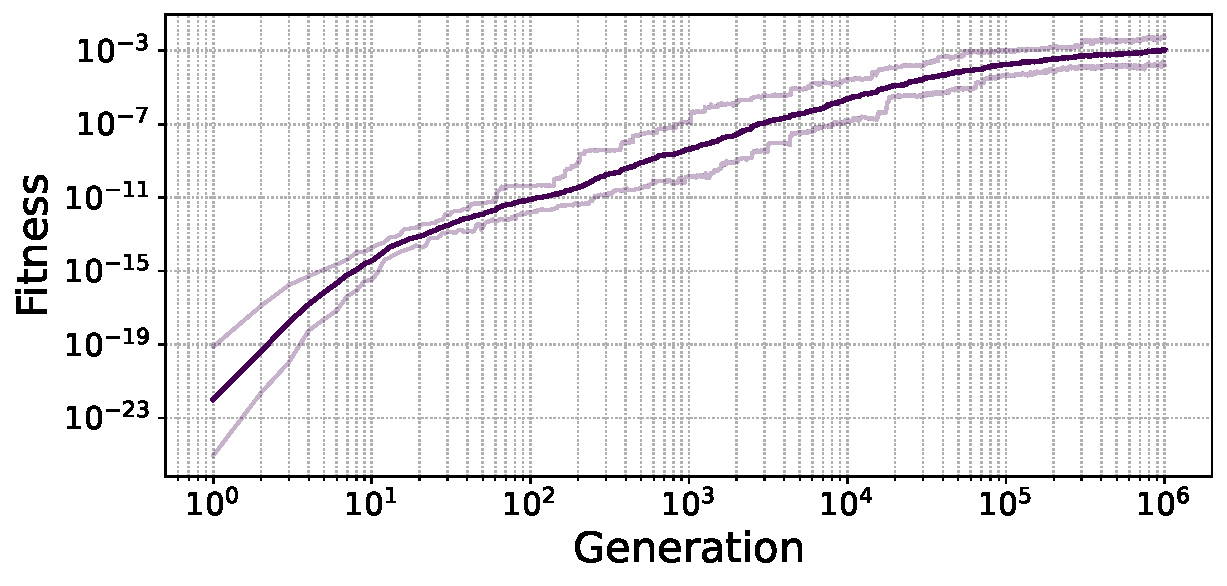
\includegraphics[width=0.75\textwidth]{ploscb/img/all_fitness.pdf}
  \caption[Average fitness during evolution in the advanced model]{Geometric average of the fitness of the best individual in each of the 30 replicates, at every generation.
  Lighter lines represent the first and last decile of the data.}
  \label{fig:ploscb:main_fitness}
\end{figure}

In our simulations, the fitness of the best individual in each population increases over evolutionary time, as shown in Figure~\ref{fig:ploscb:main_fitness}, meaning that evolution is able to select phenotypes that are closer and closer to the target. More precisely, the expression levels of the genes of each type in individuals in our model therefore evolve towards their respective targets, as previously defined in Section~\ref{sec:ploscb:evol_model}.

% Example genome in both environments
\begin{figure}[H]
  \centering
  \begin{elasticrow}[width=\textwidth]
  \elasticfigure{ploscb/img/genome_and_tsc_rep21_env_A.pdf}
  \elasticfigure{ploscb/img/genome_and_tsc_rep21_env_B.pdf}
  \end{elasticrow}
  \caption[Best individual at the end of evolution in one of the replicates in the advanced model, in both environments]{Genome of the best individual at the last generation of replicate 21, evaluated in environments A (left) and B (right).
  In addition to Figure~\ref{fig:ploscb:random_indiv}, the outer ring shows the state of each gene: dark color, activated -- light color, inhibited.
  The inner ring shows the level of transcription-generated DNA supercoiling at every position on the genome: Shades of blue represent negative supercoiling, and shades of red positive supercoiling.}
  \label{fig:ploscb:genomes}
\end{figure}

The genome of an example evolved individual at the end of the simulation is depicted in Figure~\ref{fig:ploscb:genomes}, along with its level of local supercoiling and gene activity in each environment.
Different activation patterns for each gene class are clearly visible on the genome of this individual.
Indeed, all \emph{AB} genes except one are activated (dark blue) in each environment, whereas 19 out of 20 \emph{B} genes are correctly inhibited (light green) in environment A (left) and 18 correctly activated (dark green) in environment B (right).
Conversely, 16 \emph{A} genes are activated (dark red) in environment A, and 16 inhibited (light red) in environment B.

The transcription-generated supercoiling represented in the inner ring furthermore changes consistently with the gene activation patterns between the two environments: red zones, where DNA is positively supercoiled, contain inhibited genes, whereas blue zones, where DNA is negatively supercoiled, contain activated genes.
This individual therefore shows that it is possible for evolution to adjust the gene expression levels of an individual in our model to an environment-dependent target, by relying only on the transcription-supercoiling coupling and on the relative positions of genes on the genome.

% Evolution of gene _activation_ by gene class
\begin{figure}[H]
  \begin{elasticrow}[width=\textwidth]
    \elasticfigure{ploscb/img/gene_activity_env_A_quantile.pdf}
    \elasticfigure{ploscb/img/gene_activity_env_B_quantile.pdf}
  \end{elasticrow}
  \caption[Average number of activated genes during evolution in the advanced model]{Average number of activated genes (with an expression level above $e_{1/2}$) of each type, out of 20, in the best individual at every generation, averaged over the 30 replicates, in environments A (left) and B (right).
  Lighter lines represent the first and last decile of the data.}
  \label{fig:ploscb:gene_activity_by_env}
\end{figure}

\paragraph{Evolution of Class-Specific Gene Expression Levels}
These results are however not specific to this particular individual.
Figure~\ref{fig:ploscb:gene_activity_by_env} shows that, averaging over all replicates, the number of activated genes in each class evolves towards their respective target.
In each environment, the average number of activated \emph{AB} genes quickly reaches nearly 20, its maximum value, as expected from their target; \emph{B} genes follow the same behavior, evolving towards nearly full activation in environment B and nearly full inhibition in environment A.
\emph{A} genes follow a slightly different course, as the number of activated \emph{A} genes seems to converge to approximatively 15 out of the expected 20 in environment A, but continues to decrease towards the expected 0 in environment B by the end of the simulations.

The incomplete match to their target of \emph{A} genes does however not come as a complete surprise.
Environment A is indeed characterized by a positive supercoiling shift $\delta\sigma_A > 0$, while environment B is characterized by a negative supercoiling shift $\delta\sigma_B < 0$.
As positive supercoiling hinders promoter opening, it is more difficult for a gene to have a high transcription rate in environment A than in environment B.
\emph{A} genes must therefore complete the more difficult task of being activated in the ``hard'' environment A, while being inhibited in the ``easy'' environment B.
Differentiated expression levels nonetheless evolve in our model for each type of gene, as a result of the different supercoiling levels imposed by the environmental conditions.

% Final message: evolution of hypercoiling-activated phenotype
\begin{figure}[H]
  \centering
  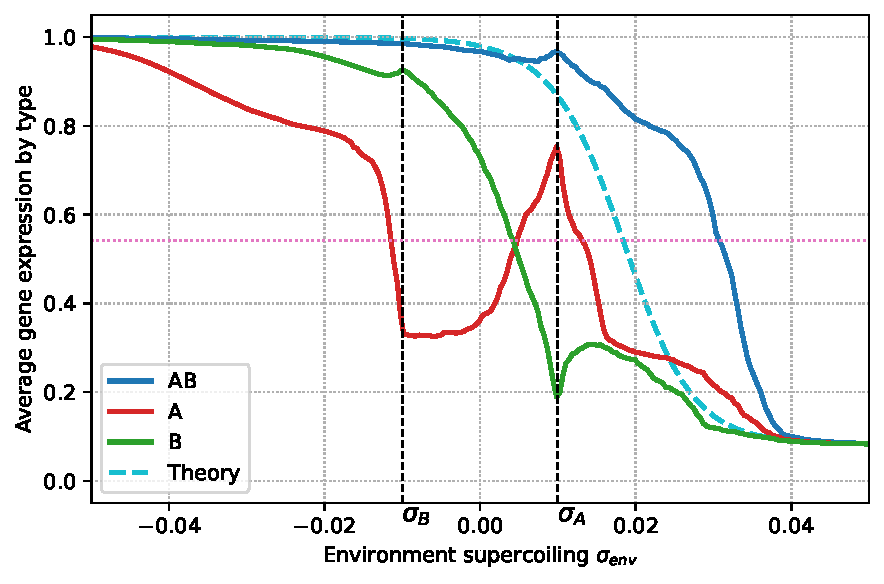
\includegraphics[width=\textwidth]{ploscb/img/activity_sigmas_avg.pdf}
  \caption[Average gene expression as a function of background supercoiling at the end of evolution in the advanced model]{Average gene expression level for each class of gene (\emph{A}, \emph{B}, and \emph{AB}), as a function of the background supercoiling level $\sigma_{basal} + \delta\sigma_{env}$, averaged over the best individual of each of the 30 replicates.
  The dash-dotted light blue line represents the average expression level of genes on a random genome, and the dashed light blue line represents the expression level of a single neighbor-less gene.
  The black vertical lines represent environments A and B, in which individuals evolve during the simulation, and the pink horizontal line marks $e_{1/2}$, the threshold above which a gene is considered active.}
  \label{fig:ploscb:activity_by_sigma}
\end{figure}

\paragraph{Evolution of Relaxation-Activated Genes}
In our model, the expression level of a gene increases exponentially with the opening free energy of its promoter, which itself increases as a sigmoidal function of negative supercoiling.
When measuring the response of an individual's genes to variation in the background supercoiling $\sigma_{basal} + \delta\sigma_{env}$, one could therefore expect a qualitatively similar response.

Figure~\ref{fig:ploscb:activity_by_sigma} shows the responses of genes of different types to the background supercoiling level (as explained in equation~\ref{eq:sigma}), and highlights striking differences between the expression of evolved, random, or isolated genes, as well as between the different gene types in evolved genomes.
The light blue lines in the figure serve as a reference point, showing the response of an isolated, non-interacting gene to environmental supercoiling (dashed line), and the average response (dash-dotted line) of genes on 30 random genomes, generated using the parameters from Table~\ref{tab:param_values}.
While \emph{AB} and \emph{B} genes (blue and green curves) display an expression level that decreases with the level of negative supercoiling, and that remains qualitatively similar to the behavior of random genes (dash-dotted line), \emph{A} genes display a completely different behavior.
These genes show a non-monotonic response to environmental supercoiling, as their expression level decreases until a local minimum in expression at $\delta\sigma_B$, then increases again even though negative supercoiling decreases until a local maximum at $\delta\sigma_A$, before decreasing again like the other kinds of genes.
In other words, \emph{A} genes present a phenotype of activation by environmental relaxation of DNA, for values between $\delta\sigma_B$ and $\delta\sigma_A$, even though the promoter activity of an isolated \emph{A} gene decreases with DNA relaxation.

The transcription-supercoiling coupling therefore provides a regulatory layer that mediates the transcriptional response to the global variation in DNA supercoiling caused by different environments.
Indeed, it remarkably allows in our model for the evolution of a response that is opposite not only to the response displayed by a non-interacting, neighborless gene, but also to the response of genes placed at random on a similar genome, demonstrating the importance of the relative position of genes on the genome.


\subsection{Evolution of Local Genome Organization}

Having characterized the different patterns of gene transcription that evolved in our simulations in response to the two different environmental conditions, we sought to determine the genome organization that necessarily underlies these patterns, since the only difference between individuals in our model is the relative position and orientation of the genes on their genome.

We started by studying genome organization at the local level, and measured the relative abundance of pairs of neighboring genes in every relative orientation: convergent, divergent, or in tandem.
The relative orientation between neighboring genes determines the mode of interaction between these genes, by applying the twin-domain model of transcription-generated supercoiling to the promoter of each gene: mutual activation for divergent genes, mutual inhibition for convergent genes, and activation (resp. inhibition) of the upstream (resp. downstream) gene by the downstream (resp. upstream) gene.

As the different gene types must evolve different activation patterns in each environment to have a high fitness in the model, we separated the pair counts by the type of each gene in the pair, resulting in 9 kinds of pairs.
Finally, in order to quantify the actual strength of the coupling between the genes in a given type of pair, we summed the total level of positive and negative supercoiling generated by the transcription of each gene in the pair at the promoter of the other gene for all relative orientations.
The results are presented in Figure~\ref{fig:ploscb:pair_results}, with the left-hand side panel showing the number of pairs of each kind, and the right-hand side panel the corresponding transcription-generated supercoiling levels.
Several patterns markedly emerge from the data.

\begin{figure}[H]
	\centering
	\begin{elasticrow}[width=\linewidth, sep=1em]
		\elasticfigure{ploscb/img/gene_pair_counts.pdf}
		\elasticfigure{ploscb/img/pos_neg_supercoiling_pairs.pdf}
	\end{elasticrow}
  \caption[Number of gene pairs and supercoiling effect per type of gene pair]{Interactions between pairs of neighboring genes.
  The left-hand side panel shows the number of pairs of each kind, split by the type of the first gene (sub-row) and of the second gene (sub-column) in the pair, and by relative orientation (bars in each sub-panel: convergent, divergent, upstream, or downstream).
  %As there are 20 genes of each type, and each gene appears in two pairs, the total number of pairs in each sub-row and sub-column is always 40.
  For instance, the top-right panel shows the influence of AB genes on B genes, and the bottom-left panel the influence of B genes on AB genes (in the same pairs).
  In that case, there are on average 7.8 \emph{AB} genes directly upstream of a \emph{B} gene (in red), or 7.8 \emph{B} genes directly downstream of an \emph{AB} gene (in green) on an evolved genome.
  % Talk about induced supercoiling?
  The right-hand side panel shows, for each kind of pair, the total amount of positive (red) and negative (green) transcription-generated supercoiling due to each gene type (sub-row) measured at the promoter of each gene type (sub-column), summing over all orientations, but in each environment.
  All data is averaged over the best individual of each of the 30 replicates, and box plots indicate the median and dispersion between the replicates.}
  \label{fig:ploscb:pair_results}
\end{figure}

% Divergent pairs: AB
\paragraph{Genomes Are Enriched in Divergent \emph{AB}/\emph{AB} Gene Pairs}
The most frequently found kind of gene pair in the evolved genomes is divergently oriented \emph{AB}/\emph{AB} pairs.
13 such pairs are found on average (see the \emph{AB}/\emph{AB} sub-panel on the left-hand side of Figure~\ref{fig:ploscb:pair_results}), out of a possible maximum of 20 (since any given gene can only be part of a single divergent pair), meaning that two-thirds of \emph{AB} genes are part of a divergent pair with another \emph{AB} gene.
The mostly divergent \emph{AB}\emph{AB} gene pairs generate an average negative supercoiling of around -0.012 at their promoters, in both environments (summing the positive and negative bars in the \emph{AB}/\emph{AB} sub-panel on the right-hand side of Figure~\ref{fig:ploscb:pair_results}).
This value is comparable in magnitude to but has the opposite sign than the shift in supercoiling caused by environment A ($\delta\sigma_A = 0.01$), showing that the interaction between neighboring genes can locally counteract the global shift in supercoiling caused by this environment in order to maintain high gene expression levels.

% Divergent pairs: A/A and B/B too, but not A/B
Genomes also contain divergent \emph{A}/\emph{A} and \emph{B}/\emph{B} gene pairs, although less frequently than divergent \emph{AB}/\emph{AB} pairs.
As both \emph{A} genes and \emph{B} genes must be conditionally expressed or inhibited depending on the environment, the unconditionally positive feedback loop resulting from a divergent orientation seems less evolutionarily favorable for \emph{A}/\emph{A} or \emph{B}/\emph{B} pairs than for \emph{AB}/\emph{AB} pairs.
Divergent \emph{A}/\emph{A} and \emph{B}/\emph{B} pairs moreover result in slightly weaker interactions (middle and bottom-right sub-panel of the right-hand side of Figure~\ref{fig:ploscb:pair_results}), in the environment in which these genes are active.
On the contrary, divergent \emph{A}/\emph{B} gene pairs are almost never found, and this is consistent with theoretical expectation, since \emph{A} and \emph{B} genes must no be expressed in the same environment.

The local organization of the genome in divergent \emph{AB}/\emph{AB} gene pairs therefore seems to be favored by evolution, as this pattern allows for a high expression of these genes in both environments, while divergent \emph{A}/\emph{B} gene pairs, which would lead to a lower fitness, are oppositely very rarely found in evolved genomes.

% Convergent pairs: A and B, mostly
\paragraph{Genomes are Enriched in Convergent \emph{A}/\emph{B} Gene Pairs}
The pattern in which \emph{B} genes appear most frequently, and \emph{A} genes very frequently (just after divergent \emph{A}/\emph{A} pairs), is in convergent \emph{A}/\emph{B} gene pairs.
In this case, each gene in the pair should theoretically inhibit the expression of the other gene.
In environment A, \emph{A} genes indeed generate an average positive supercoiling variation of 0.01 at the promoter of convergently oriented \emph{B} genes (the effect of \emph{B} genes on convergent \emph{A} genes in environment B is similar), decreasing their expression with a strength that is again comparable to the environmental change in supercoiling, whiles B genes are mostly inhibited and therefore do not impact \emph{A} genes.
In environment B, it is instead \emph{B} genes that strongly inhibit \emph{A} genes through the generation of positive supercoiling.

Convergently oriented \emph{A}/\emph{B} gene pairs therefore form toggle switches, or bistable gene regulatory circuits, in which the expression of one gene represses the expression of the other gene~\citep{gardner2000}.
In accordance with the targeted expression patterns of \emph{A} and \emph{B} genes, we therefore observe that the local organization of the genome into toggle switches, like the divergent \emph{A}/\emph{B} pairs, is favored by evolution in order to produce environment-dependent differentiated expression levels.


\subsection{Local Interactions Do Not Recapitulate the Regulatory Network}

In order to understand the extent to which the gene regulatory network generated by the transcription-supercoiling coupling can be reduced to the local organization into pairs of genes described above, we expanded our scope to study the behavior of subnetworks of neighboring genes of increasing sizes.

\begin{figure}[H]
  \centering
  %\begin{subfigure}[t]{\textwidth}
    %\centering
    %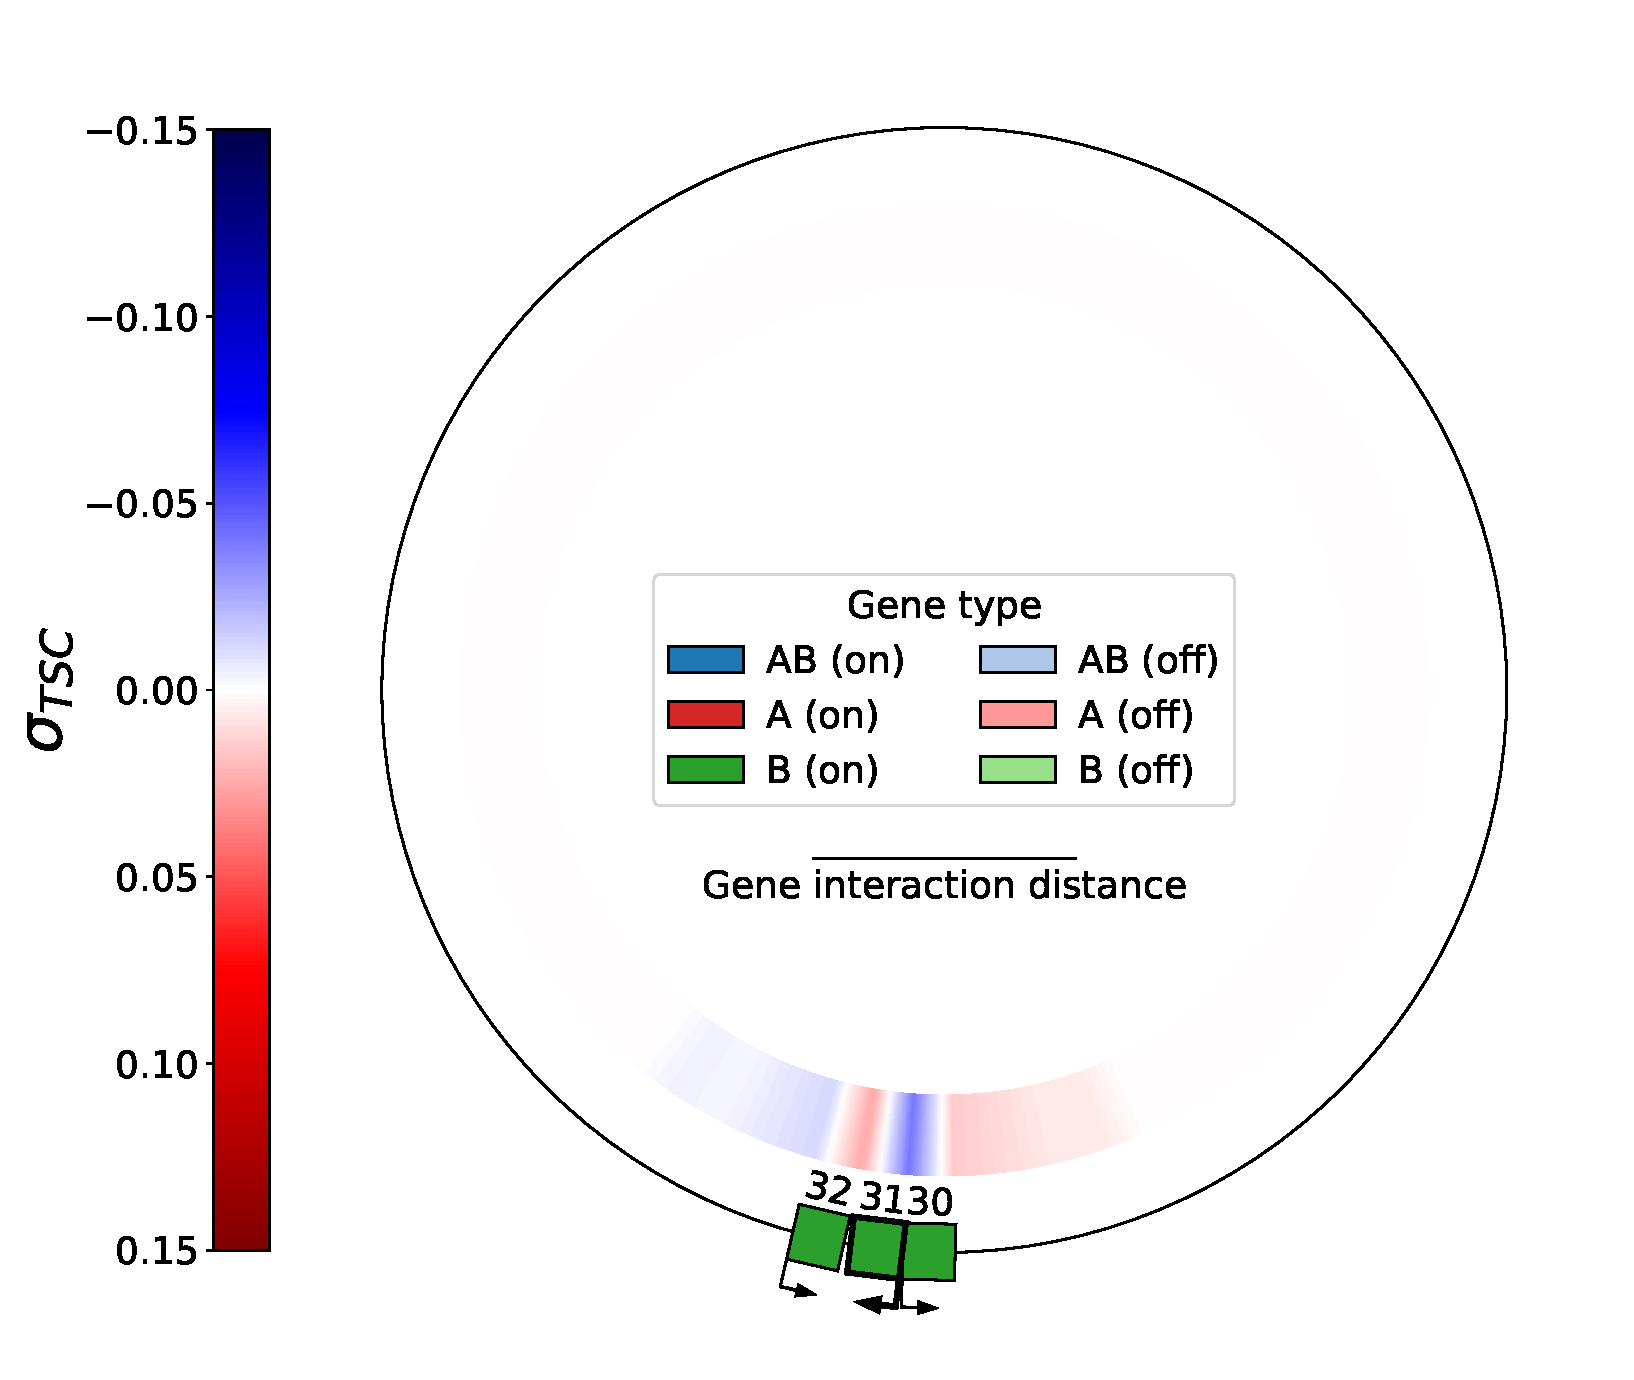
\includegraphics[height=7cm]{ploscb/img/sub_3_genes_30_env_A.pdf}
    %\hspace{-0.5cm}
    %\includegraphics[height=7cm]{ploscb/img/sub_5_genes_29_env_A.pdf}
  %\end{subfigure}
  \begin{elasticrow}[width=\linewidth]
		\elasticfigure{ploscb/img/sub_3_genes_30_env_A.pdf}
		\elasticfigure{ploscb/img/sub_5_genes_29_env_A.pdf}
	\end{elasticrow}
  \begin{elasticrow}[width=\linewidth]
		\elasticfigure{ploscb/img/sub_7_genes_03_env_B.pdf}
		\elasticfigure{ploscb/img/sub_9_genes_02_env_B.pdf}
	\end{elasticrow}
  \caption[Example minimal subnetworks needed for gene inhibition in an evolved individual]{Top: subnetworks of size 3 (left) and 5 (right) centered around gene 31 (of type \emph{B}, in bold) of the best individual at the end of replicate 21, evaluated in environment A.
  Bottom: subnetworks of size 7 (left) and 9 (right), centered around gene 6 (of type \emph{A}, in bold) of the same individual, evaluated in environment B.
  }
  \label{fig:ploscb:subnetwork_examples}
\end{figure}

For every odd subnetwork size $k$ between 1 and the genome size, and for every gene on the genome, we extracted the subnetwork of size $k$ centered around that gene, and computed the expression level of every gene in the subnetwork, in the same way as for a complete genome, in each environment.
This allowed us to compute the minimum subnetwork size at which a gene has the same activation state as in the complete genome, which we interpret as an indicator of the complexity of the interaction network necessary to produce the activation state of that gene in the complete genome.
Two representative examples are presented in Figure~\ref{fig:ploscb:subnetwork_examples}, and the complete results are then shown in Figure~\ref{fig:ploscb:min_subnetwork}.

Figure~\ref{fig:ploscb:subnetwork_examples} depicts the subnetworks that are needed in order to obtain the inhibition of a representative gene of type \emph{A} in environment B, and of a representative gene of type \emph{B} in environment A, taken from the genome of an evolved individual.
The \emph{B} gene is not inhibited by a subnetwork of size 3, but needs a subnetwork of size 5 to be inhibited, and similarly, the \emph{A} gene is not inhibited by a subnetwork of size 7, but needs a subnetwork of size 9 to be inhibited.
In each case, increasing the size of the subnetwork by two (one gene on each side) completely changes the resulting gene expression levels, alongside with the associated level of transcription-generated supercoiling.
Indeed, in the top example, all 3 genes in the small subnetwork switch states when evaluated inside the larger subnetwork, and in the bottom example, the two \emph{B} genes and two out of the three central \emph{A} genes switch activation states when moving from the small to the large subnetwork.
In these examples, the activity of a gene is therefore not only dependent on its closest neighbors, but on a quite larger section of the genome.

\begin{figure}[H]
  \centering
  \includegraphics[width=\textwidth]{ploscb/img/min_network_size.pdf}
  \caption[Minimal subnetwork size needed to obtain the correct activation state per gene type]{Minimal contiguous subnetwork size needed for the central gene in the subnetwork to have the same activation state as in the complete genome, for each gene type, and in each environment, for every gene of the best individual at the end of each replicate.
  In each case, a box plot showing quartiles and fliers is overlaid on a violin plot representing the whole distribution, and the mean is represented by a smaller tick.
  The data is computed only for genes which present the correct activation state in both environments, which represents 97,7\% of \emph{AB} genes, 92,7\% of \emph{B} genes and 53,2 \% of \emph{A} genes.}
  \label{fig:ploscb:min_subnetwork}
\end{figure}

We averaged this data over every gene that presents the correct activation state in each environment, in the best individual of every replicate, and very different patterns once more appear, depending on whether the targeted behavior for the gene is activation or inhibition, as depicted in Figure~\ref{fig:ploscb:min_subnetwork}.
For \emph{AB} genes in both environments, as well as for \emph{A} genes in environment A and \emph{B} genes in environment B, the experimentally obtained minimum subnetwork size is 1, which is consistent with the expression profile of an isolated gene, shown in Figure~\ref{fig:ploscb:activity_by_sigma}: With a basal supercoiling value of $\sigma_{basal} = -0.06$, an isolated gene already experiences a high expression level in both environments, even without interactions.

When the evolutionary target of the gene is inhibition, that is for \emph{A} genes in environment B and for \emph{B} genes in environment A, the picture is however quite different.
In this case, a significantly larger subnetwork is needed in order to obtain inhibition of the central gene: The median subnetwork size is 9 (4 genes on each side) for \emph{A} genes.
For \emph{B} genes, the median size is smaller than for \emph{A} genes, but higher than when the target is activation: Genes always need at least a subnetwork of size 3 (1 gene on each side), and several outliers need a subnetwork of more than 20 genes.

The gene regulatory networks evolved through the transcription-supercoiling coupling therefore exhibit a structure that cannot always be summarized by the pairwise interactions between neighboring genes, but that can on the contrary require the participation of a significantly larger number of genes in order to make genes display the same activation state as in the full genome.


\subsection{A Whole-Genome Gene Regulatory Network}

The effect of the transcription of every gene on the local supercoiling at every other gene (which decreases linearly with distance) provides a natural graph to represent the interactions between the genes in the genome of an individual.
However, as the effective impact of a gene on the expression of other genes depends on the transcription level of that gene, this theoretical graph provides an inaccurate picture of the gene interactions that actually take place, as every gene ends up expressed at a different level.
In order to characterize more finely the gene regulatory networks that evolve in our experiments, we therefore constructed a different graph, which we call the effective interaction graph, using transcriptional gene knockouts.

\begin{figure}[H]
  \centering
  \begin{elasticrow}[width=\linewidth]
		\elasticfigure{ploscb/img/ko_genome_and_tsc_env_A_gene_36.pdf}
		\elasticfigure{ploscb/img/ko_genome_and_tsc_env_B_gene_36.pdf}
	\end{elasticrow}
  \caption[Example evolved individual with a knocked-out gene, evaluated in both environments]{Knockout of gene 36 (of type \emph{AB}, in bold, colored white) of the best individual at the end of replicate 21, evaluated in environments A (left) and B (right).
  Hatched genes represent genes whose activation state was switched by the knockout compared to their state in the original genome.
  The inner ring represents the absolute difference in the level of local supercoiling $|\Delta\sigma_{TSC}|$ between the knockout genome and the original genome (in Figure~\ref{fig:ploscb:genomes}).}
  \label{fig:ploscb:ko_genomes}
\end{figure}

\paragraph{Transcriptional Gene Knockouts}
A transcriptional gene knockout (or simply gene knockout in the manuscript) completely suppresses the transcription of a gene, adapting the principle of gene knockouts to the transcription rather than the translation step of gene expression.
In order to knock out a gene in an individual in our model, we simply set the transcription rate of that gene to zero during every step of the computation of the gene expression levels of that individual.
This virtually removes the knocked-out gene from the genome, while keeping the intergenic distance between its upstream and downstream neighbors unchanged, and mimics a loss of function its the promoter.
The result of such a knockout on the genome of an evolved individual is shown in Figure~\ref{fig:ploscb:ko_genomes}.
The knocked-out gene is gene 36, which is of type \emph{AB} and originally activated in both environments (see Figure~\ref{fig:ploscb:genomes} for the original genome).
We can see that, in environment A, knocking out this gene results in a switch of the activation state for 7 genes (hatched in the left-hand side of Figure~\ref{fig:ploscb:ko_genomes}), that are not all contiguously located, and in local supercoiling changes that propagate to the bottom left third of the genome, to a distance that is larger than the gene interaction distance.
In environment B, knocking out this gene results in milder supercoiling changes that do not lead to the switch of any gene.
In this example, knocking out even a single gene can therefore substantially affect gene expression levels, significantly switching the activation state of other genes on the genome, even when they are out of reach of direct interaction with the knocked-out gene.

\begin{figure}[H]
  \centering
  \hspace{-1cm}
  \begin{subfigure}[c]{0.73\textwidth}
    \includegraphics[width=\textwidth]{ploscb/img/combined_effective_graph_rep21_graphviz.pdf}
  \end{subfigure}
  \hspace*{-0.75cm}
  \begin{subfigure}[c]{0.29\textwidth}
    \includegraphics[width=\textwidth]{ploscb/img/effective_graph_wcc_distr.pdf}
  \end{subfigure}
  \caption[Effective interaction graph of an evolved individual, and distribution of effective interaction graph WCCs in evolved and random individuals]{Left: effective interaction graph of the best individual at the last generation of replicate 21, obtained by knocking out each gene and measuring the resulting gene switches in each environment.
  Activation edges are drawn in green, and inhibition edges in red.
  The numbering of the genes is the same as in Figures~\ref{fig:ploscb:genomes},~\ref{fig:ploscb:ko_genomes} and~\ref{fig:ploscb:ko_genomes}.
  Right: distribution of weakly connected component (WCC) sizes in the effective interaction graphs of the evolved individuals (left) and the random individuals (right).}
  \label{fig:ploscb:ko_graph}
\end{figure}

\paragraph{Constructing Effective Interaction Graphs}
In order to construct the effective interaction graph introduced above, we simply add an edge from a gene to every other gene whose activation state is switched by knocking out that gene, in one environment or the other.
If the knockout switches off a gene that was activated in the complete genome, we mark the edge as an activation edge, meaning that the knocked-out gene was necessary to activate the switched gene.
If the knockout switches on a gene that was inhibited in the complete genome, we conversely mark the edge as an inhibition edge.
If knocking out a gene switches the same gene in the two environments, we only add the edge once (we do not build a multigraph).
The effective interaction graph of our example individual is presented on the left-hand side of Figure~\ref{fig:ploscb:ko_graph}.
In the case of this individual, there is a single weakly connected component (WCC), meaning that all genes interact as part of a single whole-genome regulatory network; this is the case in the best individual of 26 out of the 30 replicates.

\paragraph{Structure of the Effective Interaction Graphs}
We computed the effective interaction graph of the best individual in each replicate, and compared these graphs with the effective interaction graphs of 30 random individuals drawn using the same genome parameters (in Table~\ref{tab:param_values}).
The results are presented on the right-hand side of Figure~\ref{fig:ploscb:ko_graph}.
The effective interaction graphs of evolved individuals are clearly different from the interaction graphs of random individuals.
We can see that the evolved genomes have WCC sizes of 58 to 60 genes, comprising nearly every to every gene on the genome, along with very few single-gene WCCs (left).
On the other hand, WCC sizes in the random genomes span the whole range from single-gene to whole-genome WCCs, with most of the connected components counting less than 10 genes (right).

\begin{figure}[H]
  \begin{subfigure}[t]{0.49\textwidth}
    \includegraphics[width=\textwidth]{ploscb/img/effective_graph_combined_out_degree.pdf}
  \end{subfigure}
  \begin{subfigure}[t]{0.49\textwidth}
    \includegraphics[width=\textwidth]{ploscb/img/effective_graph_combined_in_degree.pdf}
  \end{subfigure}
  \caption[Average in- and out-degree of effective interaction graph nodes for evolved and random individuals]{Left: average out-degree (number of genes switched by knocking out a given gene) of the nodes in the effective interaction graph, separated by gene type, for evolved and random individuals.
  Right: average in-degree (number of genes whose knockout switches a given gene) of the nodes in the effective interaction graph, separated by gene type, for evolved and random individuals.}
  \label{fig:ploscb:ko_data}
\end{figure}

The evolved genomes are indeed much more connected than the random genomes, as we can see in Figure~\ref{fig:ploscb:ko_data}, which presents the out- and in-degree of genes (averaged by gene type) in the effective interaction graphs of the genomes.
The left-hand side of Figure~\ref{fig:ploscb:ko_data} shows the average out-degree of each gene type, or the number of genes that are switched by knocking out a gene of that type.
While knocking out a gene in a random genome switches the state of just under 2 other genes on average, the figure is much higher in the evolved genomes.
Knocking out \emph{A} and \emph{B} genes switches 4 other genes on average, and knocking out \emph{AB} genes up to 7 other genes;
\emph{AB} genes therefore play a quantitatively more important regulatory role than \emph{A} genes or \emph{B} genes, which can be explained by the fact that \emph{AB} genes are activated in both environments, while most \emph{A} and \emph{B} genes are inhibited in one environment or the other.

When looking at the in-degree of the genes, or the number of genes whose knockout will make a given gene switch activation states, we can see that the evolved genomes are again much more connected than the random genomes, and that the in-degree depends on the type of the gene.
Indeed, \emph{AB} genes are only switched by one other gene on average, meaning that their activation state is robust to perturbations in the regulatory network.
The robustness of \emph{AB} gene state is expected, as these genes must have the same activation state in both environments.
On the contrary, \emph{A} genes and \emph{B} genes have an in-degree that is much higher, meaning that their activation state relies on the regulatory action of a large number of other genes, making them more sensitive to the variations between the two environments.

The evolution of the the relative positions of genes on the genome, by leveraging the feedback loop between the transcription of neighboring genes that is mediated by DNA supercoiling, therefore results in our model in the emergence of gene regulatory networks that connect the whole genome into a single entity, rather than a juxtaposition of independent subnetworks.
The network structure that evolves furthermore allows genes to dampen, or amplify, the result of the environmental shift in supercoiling on their activation states, as required by their evolutionary targets.

\section{Discussion and Perspectives}

DNA supercoiling, through its effect on promoter activation~\citep{forquet2021}, is an important actor of the regulatory response of bacteria to changing environmental conditions~\citep{martisb.2019}.
But supercoiling itself is in return impacted by transcription, as presented in the twin-domain model of~\cite{liu1987}.
Indeed, transcription has been shown to play a major role in shaping the bacterial DNA supercoiling landscape~\citep{visser2022}.
Taken together, these observations raise the question of the extent to which the position itself of genes on the genome can regulate their activity, via the coupling of the transcription levels of neighboring genes through local changes in DNA supercoiling.

In order to assess the theoretical possibility of the evolution of such a gene regulatory network, and to determine the potential consequences of the evolution of such a network on the organization of the genome, we developed in this work an evolutionary model of the transcription-supercoiling coupling (expanding upon a proof-of-concept presented in~\cite{grohens2021}), in which populations of individuals must evolve differentiated gene expression levels in response to different environmental conditions, with the transcription-supercoiling coupling as the only regulatory mechanism and inversions as the only mutational operator.
As a the dynamic supercoiling level between actively transcribed genes would be very difficult to model quantitatively, our model voluntarily stays very simple in this regard, and focuses instead on providing a qualitative overview of the range and complexity of the regulatory interactions between neighboring genes that can be mediated by the transcription-supercoiling coupling.

We showed that, in this model, gene regulation by DNA supercoiling is indeed a sufficient mechanism to evolve environment- and gene-specific patterns of activation and inhibition.
In particular, we observed the emergence of genes that are more expressed in a relaxation-inducing environment (or relaxation-activated genes), even though this behavior goes against the facilitated opening of the -10 promoter element by RNA polymerase during the initiation of transcription~\citep{forquet2021}.
%, and is accordingly quite unfrequent in \emph{in vitro} transcription data (where isolated promoters are expressed on plasmids).
This property has been analyzed in detail \emph{in vivo} in the classical example of the \emph{gyrA} promoter, and was shown to result from the unusual sequence of that promoter~\citep{menzel1987}, but for many other genes, this property is less firmly established and depends on the experimental conditions, with experiments finding a proportion of relaxation-activated genes varying between 27\% and 70\% in \emph{S. enterica}~\citep{pineau2022a}.
Our results demonstrate that this behavior can result not only from the specific sequence of the promoter (as for the \emph{gyrA} promoter), but also from the local genomic organization (as suggested in~\cite{elhoudaigui2019}), and confirm the importance of this additional mode of regulation for the first time in an evolutionary simulation.
%A global relaxation of DNA can indeed result in the local hypercoiling, and hence high expression, of genes that happen to be located in the right genetic context.
%The regulation of gene expression by local changes in DNA supercoiling therefore provides a possible causal mechanism for the activity of the relaxation-activated genes found in \emph{E. coli}~\citep{peter2004,sobetzko2016}, \emph{S. enterica}~\citep{webber2013}, or \emph{D. dadantii}~\citep{pineau2022}.

We found that evolved genomes in the model are enriched in divergent pairs of always-active genes, as well as in convergent pairs that act as bistable toggle switches~\citep{gardner2000,johnstone2022}; the evolution of such systems substantiates the theoretical predictions made by models that explicitly describe the movement of RNA polymerases during gene transcription, such as~\cite{sevier2021}.
Then, we showed that the local organization of the genome into convergent or divergent pairs of genes is not sufficient to explain the transcriptional response of individuals to different environments, but that larger subnetworks can be required to selectively inhibit genes in specific environments.
Such regulation of gene expression through interaction with groups of neighboring genes could help explain the evolutionary persistence of synteny groups between \emph{E. coli} and \emph{S. enterica}~\citep{junier2016}, as well as through the evolutionary history of \emph{B. aphidicola}~\citep{brinza2013}.
Indeed, we show that local interactions can play a role in regulating the expression of neighboring genes, and genomic rearrangements might disrupt these local interactions.
Finally, we used transcriptional knockouts, adapting the  classical tool of gene knockouts~\citep{baba2006} to our transcription-centric model, in order to characterize the evolved gene regulatory networks in further detail.
We first showed that these regulatory networks integrate the entire genome of evolved individuals into a single connected unit, in opposition to the sparser, disconnected regulatory networks displayed by randomly generated individuals.
Then, we showed that the structure of these networks leverages the transcription-supercoiling coupling to increase or decrease the sensitivity of genes to perturbations in the regulatory network, strengthening the differentiated expression patterns that are the evolutionary target for each gene type.

All in all, our simulations demonstrate that the transcription-supercoiling coupling provides a regulatory mechanism that is precise enough for the evolution of complex regulation patterns that only depend on the arrangement of genes on the genome.

Several work directions still remain open to investigation.
From an evolutionary perspective, the experimental framework in which we tested our model is at present very simple, and could be extended.
The desired gene expression levels in our model are binary, targeting maximal or minimal transcription, but could be replaced by an arbitrary level between these values for each gene, in order to see whether the local organization into pairs as well as the whole-genome regulatory network that we described are preserved under these less constrained conditions.
Similarly, we could refine the environmental challenge faced by individuals by evaluating them in each environment in succession, rather than separately, or by continuously changing the environment over evolutionary time.
From a theoretical perspective, a range of mechanistic biophysical models of the transcription-supercoiling coupling have been put forward, with different hypotheses underpinning the coupling:~\cite{brackley2016} shows a phase transition in the transcription regime as the number of transcribing RNA polymerases increases;~\cite{sevier2021} shows that bursty transcription can emerge from the transcription-supercoiling coupling; and~\cite{meyer2014} and~\cite{elhoudaigui2019} try to predict gene expression levels quantitatively from the local DNA supercoiling level.
An important vindication of these theoretical approaches to the interplay between supercoiling and transcription would therefore be to verify the extent to which these models, including ours, conform to one another as the level of abstraction changes.
Moreover, integrating a model of gene regulation by DNA supercoiling into a more comprehensive evolutionary model of the genome that allows for classical gene regulation via transcription factors, such as the model presented in~\cite{crombach2008}, would help shed light on the coevolution between the different modes of gene regulation that are available to bacterial genomes.
Finally, from an experimental perspective, a better understanding of the regulatory interactions caused by the transcription-supercoiling coupling could help design more reliable synthetic genetic constructs, as explored in~\cite{johnstone2022}.


\section{Conclusion}

To the best of our knowledge, our work is the first to model the regulatory role of supercoiling on transcription at a many-gene scale, using evolutionary simulations.
It demonstrates the importance of the direct interactions between genes that are mediated by local changes in DNA supercoiling on their transcription rates, as well as the precision and versatility of the regulatory activity stemming from these interactions.
For experimentalists, it provides an underlying theory that could help explain the heterogeneous transcriptomic response (with both up- and down-regulation of multiple genes) observed in bacteria confronted to supercoiling variations, due among others to virulence-inducing environments~\citep{dorman2019} or to gyrase-inhibiting antibiotics~\citep{delacampa2017}.
For evolutionists, it provides a plausible evolutionary rationale for the observed conservation of local gene order between closely related bacteria~\citep{junier2016} and along evolutionary histories~\citep{brinza2013}.
Finally, for synthetic biologists, it provides a theory to help predict in finer detail the gene transcription levels that can be expected from a given gene syntax~\citep{johnstone2022}, which could help design more robust genetic circuits.

\chapter{Evaluating the Robustness of the \emph{EvoTSC} Model}
\label{chap:param}

In this chapter, I explore the robustness of the characteristics of evolving populations to variations in the parameters of the \emph{EvoTSC} model.
To this aim, I present several sets of additional evolutionary simulations.
In these simulations, I first measure whether populations are able to evolve differentiated gene expression patterns as a response to different environments in the model variants.
I then compare the speed of evolution of these populations with the main runs presented in Chapter~\ref{chap:ploscb}.
I first explore the sensitivity of the model to the genome-level parameters (see Table~\ref{tab:param:params} below): the maximum interaction distance for the transcription-supercoiling coupling, the mean intergenic distance, and the strength of the environment-caused shift in background supercoiling.
I then investigate simulating a higher number of genes on the genome.
Finally, I discuss the evolutionary effect of allowing intergenic distances to mutate, by introducing indels in intergenic sections as a new mutational operator in the model.
The data from this experiment is available online on the \href{https://doi.org/10.5281/zenodo.7304906}{Zenodo} platform.

\begin{table}[H]
\begin{center}
\begin{tabular}{l c r r}
\toprule
\textbf{Parameter} & \textbf{Symbol} & \textbf{Value} & \textbf{\# of Replicates} \\
\midrule
Interaction distance & $d_{max}$ & \textbf{5 kb} & \textbf{30}\\
(Section~\ref{sec:param:inter25k}) & & 25 kb & 15\\
\midrule
& & 10 bp& 15\\
Mean intergenic size & $d_{mean}$ & \textbf{125 bp} & \textbf{30} \\
(Section~\ref{sec:param:mean-intergene})& & 1,000 bp & 15\\
& & 10,000 bp & 15 \\
\midrule
& & 0.0001 & 15\\
Environment supercoiling shift & $\delta\sigma_{A/B}$ & 0.001 & 15\\
(Section~\ref{sec:param:sigma-env})& & \textbf{0.01} & \textbf{30}\\
%\midrule
%Number of genes & $n$ & \textbf{60} & \textbf{30} \\
%(Section~\ref{sec:param:300-genes})& & 30 & 15 \\
\bottomrule
\end{tabular}
\end{center}
\caption[Table of parameter values explored in additional \emph{EvoTSC} simulations]{Table of the parameters and associated values explored in additional experiments (separated by horizontal lines).
For each experiment, the row in bold font corresponds to the parameter values used in the main run described in Chapter~\ref{chap:ploscb}, and is shown for reference.}
\label{tab:param:params}
\end{table}

\section{Interaction Distance}
\label{sec:param:inter25k}

The size of the topological domains of bacterial genomes, inside which DNA supercoils can freely propagate, has historically been estimated to be on the order of a few thousand base pairs~\citep{elhanafi2000,postow2004,kouzine2013}.
Recent work has however suggested that the size of transcription-generated twin domains could be much larger than this, and reach up to 25 kb on either side of the transcribed gene~\citep{visser2022}.
As the size of the topological domains sets a limit to the number of genes that can interact through the transcription-supercoiling coupling, it is likely to play an important role in the structure of the supercoiling-mediated gene regulatory networks.
By increasing the number of genes a given gene is coupled with, a larger interaction distance could make genomic inversions more deleterious by making them disrupt a larger part of the regulatory networks at their boundaries, but it could also allow more robust regulatory networks to evolve through a higher connectivity.
In this section, I present simulations run with an interaction distance of 25 kb, a five-fold increase from the value used in the main runs, in order to test these hypotheses.

\begin{figure}[H]
\centering
\includegraphics[width=0.495\textwidth]{param/interaction-25k/gene_activity_env_A.pdf}
\includegraphics[width=0.495\textwidth]{param/interaction-25k/gene_activity_env_B.pdf}
\caption[Evolution of the number of activated genes in each environment, with an interaction distance of 25 kb]{Evolution of the number of activated genes in environment A (left) and environment B (right), with an interaction distance of 25 kb.
Lighter lines represent the first and last decile of the data.}
\label{fig:param:inter25k-activ-by-env}
\end{figure}

Figure~\ref{fig:param:inter25k-activ-by-env} shows the evolution of the number of activated genes of each type in the simulations with the interaction distance of 25 kb, over 250,000 generations (to be compared to Figure~\ref{fig:ploscb:gene_activity_by_env} in Chapter~\ref{chap:ploscb}).
As in the main run, the number of activated genes of each type evolves towards their respective target.
Differentiated activation patterns can therefore still evolve even when the topological domains are 5 times larger.

\begin{figure}[H]
\centering
\includegraphics[width=0.8\textwidth]{param/interaction-25k/fitness_all_with_main.pdf}
\caption[Average fitness during evolution, with an interaction distance of 25 kb]{Average fitness during evolution with an interaction distance of 25 kb (light blue), and in the main run (dark blue).
Lighter lines represent the first and last decile of the data.}
\label{fig:param:inter25k-fitness}
\end{figure}

Figure~\ref{fig:param:inter25k-fitness} shows the evolution of the average fitness of the best individual in each replicate of the simulation with a larger interaction distance, compared with the evolution of fitness in the main run, over 250,000 generations.
While fitness is systematically lower throughout evolution with the larger interaction distance, it nonetheless follows a qualitatively similar curve, and keeps on increasing until the end of the runs, suggesting that it could eventually reach the same value as in the main run (presented in full in Figure~\ref{fig:ploscb:main_fitness}).

\begin{figure}[H]
\centering
\includegraphics[width=0.9\textwidth]{param/interaction-25k/activity_sigmas_avg.pdf}
\caption[Average gene expression as a function of background supercoiling, with an interaction distance of 25 kb]{Average gene expression by type as a function of background supercoiling, with an interaction distance of 25 kb.
The dash-dotted line represents the average expression of genes on a random genome with an interaction distance of 25 kb.}
\label{fig:param:inter25k-activ-by-sigma}
\end{figure}

Figure~\ref{fig:param:inter25k-activ-by-sigma} shows the average gene expression by type of evolved individuals, as a function of the background supercoiling level.
As in the main run, \emph{A} genes display a relaxation-activated phenotype.
\emph{AB} and \emph{B} genes are relaxation-inhibited, but nonetheless display quite different behaviors than the (dash-dotted light blue) curve for genes on a random genome with the same parameters, which present a much flatter response curve to background supercoiling than with the default interaction distance of 5 kb (shown in Figure~\ref{fig:ploscb:activity-by-sigma}).

\begin{figure}[H]
\centering
\includegraphics[width=0.9\textwidth]{param/interaction-25k/random_activ_per_sigma.pdf}
\caption[Average gene expression as a function of background supercoiling, with increasing interaction distances, in random genomes]{Average gene expression as a function of background supercoiling in random genomes with increasing interaction distances (full lines), and theoretical expression level of an isolated gene (dashed line).}
\label{fig:param:inter25k-random-activ-by-sigma}
\end{figure}

Comparing the effect of background supercoiling variation on the transcriptional activity of genes on random genomes with an interaction distance of 5 kb (Figure~\ref{fig:ploscb:activity-by-sigma}) or 25 kb (Figure~\ref{fig:param:inter25k-activ-by-sigma}) seems to indicate that a larger interaction distance buffers the effect of the background supercoiling on gene expression in the model.
In order to test this hypothesis, I measured the average gene expression as a function of background supercoiling in random genomes with maximum interaction distances ranging from 1 kb to 50 kb, with an average intergenic distance remaining constant at 125 bp.
For each interaction distance, I generated 100 genomes, and made each genome undergo 100 replication events to shuffle the genes on the genome via genomic inversions.
Figure~\ref{fig:param:inter25k-random-activ-by-sigma} shows the result of this experiment.
As the interaction distance increases, the response curve of genes to a changing background supercoiling level indeed becomes flatter and flatter, which can be interpreted as a buffering of the effect of the environmental perturbation on gene expression by the supercoiling-mediated interaction of a higher and higher number of genes.
Conversely, as the interaction distance gets closer to zero, the curve is closer and closer to that of an isolated, non-interacting gene.


\begin{figure}[H]
\centering
\begin{subfigure}[t]{0.495\textwidth}
\includegraphics[width=\textwidth]{param/interaction-25k/effective_graph_combined_in_degree.pdf}
\end{subfigure}
\begin{subfigure}[t]{0.495\textwidth}
\includegraphics[width=\textwidth]{param/interaction-25k/effective_graph_combined_out_degree.pdf}
\end{subfigure}
\caption[Average in- and out-degree of effective interaction graph nodes, with an interaction distance of 25 kb]{Average out-degree (left) and in-degree (right) of the genes in the effective interaction graph, separated by gene type, for individuals with an interaction distance of 5 kb (main run) or 25 kb.}
\label{fig:param:inter25k-degree}
\end{figure}

Figure~\ref{fig:param:inter25k-degree} finally presents the average in- and out-degree of the genes in the effective interaction graph obtained with gene knockouts, compared to the same data from the main run.
As could be expected, the gene regulatory networks are much more connected with the larger interaction distance, but the behavior for each gene type remains qualitatively the same as in the main run.

Overall, the evolution of supercoiling-mediated gene regulatory networks that are able to show environment-specific activation patterns, and in particular relaxation-activated genes, therefore seems robust in our model to a larger interaction distance.
Even when the networks are more densely connected, buffering gene expression, the reorganization of the genome via genomic inversion allows for specific behaviors for each gene type.


\section{Mean Intergenic Size}
\label{sec:param:mean-intergene}

In the main run, I set the initial intergenic distance between every gene to 125 bp, or a gene density of 88\%, representing the average \emph{E. coli} intergenic distance~\citep{postow2004}.
Bacteria actually present a wider range of gene densities, from 51\% in \emph{Sodalis glossinidius}, a bacteria that is undergoing massive pseudogenization after recently adopting an endosymbiotic lifestyle~\citep{toh2006}, up to 95\% in \emph{Thermotoga maritima}, an extremophile bacteria living in heated marine sediment~\citep{nelson1999}.
Like the interaction distance, the mean intergenic distance plays a role in the connectivity of the gene regulatory networks that stem from the transcription-supercoiling coupling: when the mean intergenic distance is small, more genes can on average be affected by the transcription of any given gene.
Conversely, when the mean intergenic distance is large compared to the interaction distance, the emergence of regulatory subnetworks isolated from each other by large intergenic regions becomes possible.
In this section, I test the robustness of the results with regard to the range of gene densities found across living organisms.
I present simulations with mean intergenic distances increasing logarithmically from 10 bp (or a gene density of 99\%), comparable to the median intergenic distance of 3 bp found in \emph{Pelagibacter ubique}, a free-living marine bacteria~\citep{giovannoni2005}, up to 10 kb (or a gene density of 10\%), akin to the gene-scarce eukaryotic genomes~\citep{davilalopez2010}.

\begin{figure}[H]
\centering
\includegraphics[width=0.495\textwidth]{param/mean-intergene/inter-0.01k/gene_activity_env_A.pdf}
\includegraphics[width=0.495\textwidth]{param/mean-intergene/inter-0.01k/gene_activity_env_B.pdf}

\includegraphics[width=0.495\textwidth]{param/mean-intergene/inter-0.125k/gene_activity_env_A.pdf}
\includegraphics[width=0.495\textwidth]{param/mean-intergene/inter-0.125k/gene_activity_env_B.pdf}

\includegraphics[width=0.495\textwidth]{param/mean-intergene/inter-1k/gene_activity_env_A.pdf}
\includegraphics[width=0.495\textwidth]{param/mean-intergene/inter-1k/gene_activity_env_B.pdf}

\includegraphics[width=0.495\textwidth]{param/mean-intergene/inter-10k/gene_activity_env_A.pdf}
\includegraphics[width=0.495\textwidth]{param/mean-intergene/inter-10k/gene_activity_env_B.pdf}
\caption[Evolution of the number of activated genes in each environment, with increasing mean intergenic distances]{Average number of activated genes per gene type in environment A (left) and B (right) during evolution, for average intergenic sizes from top to bottom of 10 bp, 125 bp (main run), 1 kb, and 10 kb.
Lighter lines represent the first and last decile of the data.}
\label{fig:param:mean-intergene-activ-by-env}
\end{figure}

Figure~\ref{fig:param:mean-intergene-activ-by-env} shows the evolution of the number of activated genes for each gene type in each environment, with mean intergenic distances increasing from top to bottom, for 250,000 generations.
For intergenic distances of 10 bp and 1 kb, the number of activated genes converges towards the target in each environment, as in the main run (which has a mean intergenic distance of 125 bp).
For a mean intergenic distance of 10 kb, the behavior is however qualitatively different.
While \emph{AB} genes and \emph{B} genes evolve towards the correct activation state in each environment, the proportion of activated \emph{A} genes stays close to 50\% in each environment, showing that \emph{A} genes do not evolve a well-differentiated expression pattern depending on the environment.

\begin{figure}[H]
\centering
\includegraphics[width=0.8\textwidth]{param/mean-intergene/fitness_all_with_main.pdf}
\caption[Average fitness during evolution, with increasing mean intergenic distances]{Average fitness during evolution for average intergenic distances of 10 bp, 125 bp (main run), 1 kb, and 10 kb.
Lighter lines represent the first and last decile of the data.}
\label{fig:param:mean-intergene-fitness}
\end{figure}

Figure~\ref{fig:param:mean-intergene-fitness} shows the evolution of the average fitness of the best individual in each replicate of the simulations, for each value of the mean intergenic distance, including the main run for comparison.
It confirms the results seen in the previous figure: for intergenic distances from 10 bp to 1 kb, populations evolve successfully towards differentiated gene activation patterns.
For an intergenic size of 10 kb (in light blue), however, fitness increases much more slowly, and seems to converge towards a much smaller value.

\begin{figure}[H]
\centering
\includegraphics[width=0.9\textwidth]{param/mean-intergene/inter-10k/activity_sigmas_avg.pdf}
\caption[Average gene expression as a function of background supercoiling, with an intergenic distance of 10 kb]{Average gene expression as a function of background supercoiling, with an intergenic distance of 10 kb.}
\label{fig:param:mean-intergene-10kb-activ-by-sigma}
\end{figure}

Figure~\ref{fig:param:mean-intergene-10kb-activ-by-sigma} shows the average gene activity as a function of background supercoiling, for the best individual in each of the replicates with a mean intergenic distance of 10 kb.
In this case, we do not observe the clear relaxation-activated phenotype for \emph{A} genes that was present in the main simulation.
Instead, the average expression level of \emph{A} genes is indeed slightly lower in environment B than in environment A, but remains close to half expression for background supercoiling values between -0.08 and -0.05; on the contrary, both \emph{B} and \emph{AB} genes display expression curves that closely match their respective targets.
Note also that, with an intergenic distance of 10 kb, the average activity of genes on random genomes is almost identical to that of an isolated gene (as could be expected).

\begin{figure}[H]
\centering
\includegraphics[width=0.9\textwidth]{param/mean-intergene/random_activ_per_sigma.pdf}
\caption[Average gene expression as a function of background supercoiling, with increasing mean intergenic distances, in random genomes]{Average gene expression as a function of background supercoiling in random genomes with increasing mean intergenic distances (full lines), and theoretical expression level of an isolated gene (dashed line).}
\label{fig:param:mean-intergene-random-activ-by-sigma}
\end{figure}

Figure~\ref{fig:param:mean-intergene-random-activ-by-sigma} shows the expression level as a function of background supercoiling for genes on random genomes with increasing mean intergenic distances.
For distances from 10 bp to 1 kb, the curves are qualitatively similar to one another, and quite different to the expression of an isolated, non-interacting genes.
In particular, gene expression levels are sensibly lower than the maximum in both environment A and environment B.
On the other hand, for a mean intergenic distance of 10 kb (in light blue), genes behave very closely to an isolated gene, and are all almost fully activated in both environments.
This behavior is also visible in Figure~\ref{fig:param:mean-intergene-activ-by-env} (bottom row) at the beginning of evolution, and explains the initially much lower fitness at an intergenic distance of 10 kb compared to the other values in Figure~\ref{fig:param:mean-intergene-fitness}.

Several hypotheses could explain the incomplete fulfillment of the evolutionary target in simulations with a mean intergenic distance of 10kb.
First, individuals begin evolution at a much lower fitness with a mean intergenic distance of 10 kb.
This initial impediment however does not explain why the number of activated \emph{A} genes remains similar in both environments throughout evolution, contrary to the other runs.
Another possible explanation could come from the mutational operator -- genomic inversions -- used during evolution.
As the endpoints of the genomic inversions are chosen by picking two bases uniformly at random in the intergenic regions, the number of fully neutral inversions increases with the size of these regions.
Indeed, if the two endpoint of an inversion fall in regions that are not within interaction distance of any gene, the inverted region does not interact with the rest of the genome, and the inversion is therefore completely neutral.
The increased proportion of neutral mutations when the intergenic distance is too large could make the exploration of the fitness landscape more difficult for populations, by creating hard to cross fitness valleys or plateaus between fitness peaks.
There is indeed no theoretical reason why genomes with large intergenic distances could not reach comparable fitnesses to the other intergenic distances in the mode, as a genome in which most of the intergenic content is compacted into a single intergenic region would have a qualitatively similar behavior, except for the few bordering genes on each side, to the same genome with a short intergenic region in the same position.

Evolution of gene regulation by supercoiling is therefore overall resilient to the range of gene densities seen in bacteria, but the evolution of relaxation-activated genes breaks down at the lower gene densities that are more characteristic of eukaryotes.


\section{Environmental Shift in Supercoiling}
\label{sec:param:sigma-env}

In the model, the environmental shifts in supercoiling $\sigma_A$ and $\sigma_B$ represent the effect of external stresses, such as salt shock, or pH or temperature changes, on the DNA supercoiling level, as they affect for example topoisomerase activity.
In this section, I tested the robustness of the evolution of differentiated expression levels when the shift in supercoiling caused by the environment $\sigma_A$ and $\sigma_B$ is 10 times and 100 times smaller than in the main run, i.e. when the stress is of a lower intensity.
The approach is similar to the one presented in Section~\ref{sec:alife:param_explor}, which however uses the proof-of-concept version of the model.

\begin{figure}[H]
\centering
\includegraphics[width=0.495\textwidth]{param/sigma/sigma-1e-3/gene_activity_env_A.pdf}
\includegraphics[width=0.495\textwidth]{param/sigma/sigma-1e-3/gene_activity_env_B.pdf}

\includegraphics[width=0.495\textwidth]{param/sigma/sigma-1e-4/gene_activity_env_A.pdf}
\includegraphics[width=0.495\textwidth]{param/sigma/sigma-1e-4/gene_activity_env_B.pdf}
\caption[Evolution of the number of activated genes in each environment, with decreasing environmental supercoiling shifts]{Evolution of the number of activated genes in environment A (left) and environment B (right), with environmental supercoiling shifts $\sigma_A = 10^{-3}$ and $\sigma_B = -10^{-3}$ (top) and $\sigma_A = 10^{-4}$ and $\sigma_B = -10^{-4}$ (bottom).
Lighter lines represent the first and last decile of the data.}
\label{fig:param:sigma-activ-by-env}
\end{figure}

Figure~\ref{fig:param:sigma-activ-by-env} shows the evolution of the number of activated genes for each gene type in each environment, with environmental shifts in supercoiling 10 times smaller than the main run (top) and 100 times smaller (bottom), for 250,000 generations.
In both cases, differentiated gene expression patterns evolve, although evolution seems to be slower when $\sigma_A$ and $\sigma_B$ are 100 times smaller than in the main run.
This shows that evolution of different gene expression levels as a response to externally-induced perturbations in the supercoiling level can therefore take place even when these perturbations are very minute compared to translation-generated supercoiling, and reinforces the plausibility of the hypothesis that DNA supercoiling can be used as an sensory device for the regulation of gene expression in response to environmental stress.

\begin{figure}[H]
\centering
\includegraphics[width=0.8\textwidth]{param/sigma/fitness_all_with_main.pdf}
\caption[Average fitness during evolution, with decreasing environmental supercoiling shifts]{Average fitness during evolution, with environmental shifts in supercoiling logarithmically decreasing in absolute value: $\sigma_A = 10^{-2}$ and $\sigma_B = -10^{-2}$ (main run), $\sigma_A = 10^{-3}$ and $\sigma_B = -10^{-3}$ (10 times smaller than in the main run) and $\sigma_A = 10^{-4}$ and $\sigma_B = -10^{-4}$ (100 times smaller than the main run).
Lighter lines represent the first and last decile of the data.}
\label{fig:param:sigma-fitness}
\end{figure}

Figure~\ref{fig:param:sigma-fitness} shows the evolution of the average fitness of the best individual in each replicate, for each pair of environmental supercoiling values.
It confirms the results seen in the previous figure: fitness keeps increasing throughout the simulation in all cases, but more slowly when the environmental perturbation is the smallest.

\begin{figure}[H]
\centering
\includegraphics[width=0.9\textwidth]{param/sigma/sigma-1e-3/activity_sigmas_avg.pdf}
\caption[Average gene expression as a function of background supercoiling, with an absolute environmental supercoiling shift of 0.001]{Average gene expression as a function of background supercoiling, with environmental supercoiling shifts $\sigma_A = 10^{-3}$ and $\sigma_B = -10^{-3}$.}
\label{fig:param:sigma-1e-3-activ-by-sigma}
\end{figure}

Figure~\ref{fig:param:sigma-1e-3-activ-by-sigma} shows the average gene expression per gene type as a function of background supercoiling, for the best individuals at the end of evolution with environmental shifts in supercoiling of $\sigma_A = 10^{-3}$ and $\sigma_B = -10^{-3}$.
Even though the difference between the two environments is 10 times smaller than in the main run, \emph{A} genes are still able to evolve a relaxation-activated phenotype, and \emph{B} genes are still able to quickly transition from high activation to high inhibition in a much shorter range of supercoiling values.

\begin{figure}[H]
\centering
\includegraphics[width=0.9\textwidth]{param/sigma/sigma-1e-4/activity_sigmas_avg.pdf}
\caption[Average gene expression as a function of background supercoiling, with an absolute environmental supercoiling shift of 0.0001]{Average gene expression as a function of background supercoiling, with environmental supercoiling shifts $\sigma_A = 10^{-4}$ and $\sigma_B = -10^{-4}$.
The inset at the top right of the figure shows a 150x zoom on supercoiling shift values near zero.}
\label{fig:param:sigma-1e-4-activ-by-sigma}
\end{figure}

Figure~\ref{fig:param:sigma-1e-4-activ-by-sigma} similarly shows average gene expression per gene type as a function of background supercoiling, this time with environmental supercoiling shifts $\sigma_A = 10^{-4}$ and $\sigma_B = -10^{-4}$.
Strikingly, \emph{A} genes and \emph{B} genes are still able to evolve different expression levels in the two environments, even though they are 100 times closer than in the original experiment (see the inset for the precise expression levels between $\sigma_B$ and $\sigma_A$).
Even when the environments have an effect that is around 100 times smaller than the transcription-generated supercoiling (see Figure~\ref{fig:ploscb:genomes} for an example genome and the associated transcription-generated supercoiling values), the gene regulatory networks that evolve in the simulations are still able to separate the different environments and lead gene expression levels to very different states.

These results further confirm the results of the parametric exploration of the proof-of-concept version of \emph{EvoTSC}, at the end of Chapter~\ref{chap:alife}.
They show that perturbations that have little to no effect either on an isolated gene, or on a random genome (averaging over every gene), can be picked up and amplified by supercoiling-mediated gene regulatory networks, and result in clearly differentiated gene expression levels.


\section{Number of Genes}
\label{sec:param:300-genes}

All the simulations presented up to now were run with $n = 60$ genes on the genomes of individuals.
Although genes in our model correspond to transcriptional units, and could describe operons that contain multiple genes, this number remains much lower than the real number of genes in bacteria, which ranges from the 482 protein-coding genes found in \emph{Mycoplasma genitalium}, the bacteria with the smallest-known genome~\citep{glass2006}, up to over 9,000 predicted genes in \emph{Sorangium cellulosum}~\citep{schneiker2007}.
At first sight, increasing the total number of genes in the model should not qualitatively change the simulation results, as with a genome size of 60, genes already only interact via the transcription-supercoiling coupling with a small proportion of the genome.
In order to verify this hypothesis, I ran simulations with $n = 300$ genes, with maximum supercoiling interaction distances of $d_{max} =$ 5~kb (the value used in the main runs) and $d_{max} =$ 25 kb.
As the algorithmic complexity of the \emph{EvoTSC} scales quadratically with the number of genes, the simulations were run for 100,000 generations only to keep their execution time manageable, but the simulations already show qualitative results by that time.

\begin{figure}[H]
\centering
\includegraphics[width=0.495\textwidth]{param/300-genes/interaction-5k/gene_activity_env_A.pdf}
\includegraphics[width=0.495\textwidth]{param/300-genes/interaction-5k/gene_activity_env_B.pdf}

\includegraphics[width=0.495\textwidth]{param/300-genes/interaction-25k/gene_activity_env_A.pdf}
\includegraphics[width=0.495\textwidth]{param/300-genes/interaction-25k/gene_activity_env_B.pdf}
\caption[Evolution of the number of activated genes in each environment, with a 300-gene genome]{Evolution of the number of activated genes in environment A (left) and environment B (right), with a genome containing 300 genes, and an interaction distance of 5 kb (top) and 25 kb (bottom).
Lighter lines represent the first and last decile of the data.}
\label{fig:param:300genes-activ-by-env}
\end{figure}

Figure~\ref{fig:param:300genes-activ-by-env} shows the evolution of the number of activated genes of each type in each environment, for populations of individuals with a 300-gene genome, for 100,000 generations.
While these simulations lasted only for 100,000 simulations, the evolutionary trajectories are already different from the ones taken by the main run (in Figure~\ref{fig:ploscb:gene_activity_by_env}).
Different numbers of activated genes evolve in each case as a function of the environment supercoiling, but the patterns differ depending on the interaction distance.
With the shorter interaction distance, the number of activated genes of each type seems to plateau after about 10,000 generations (top).
On the contrary, evolution seems to continue by the end of the runs for the wider interaction distance (bottom).

\begin{figure}[H]
\centering
\includegraphics[width=0.8\textwidth]{param/300-genes/fitness_all_with_main.pdf}
\caption[Average fitness during evolution, with a 300-gene genome]{Average fitness during evolution, with a 300-gene genome, and an interaction distance of 5 kb or 25 kb.
Lighter lines represent the first and last decile of the data.}
\label{fig:param:300gene-fitness}
\end{figure}

Figure~\ref{fig:param:300gene-fitness} shows the evolution of the average fitness of the best individual in each replicate of the simulations with 300 genes per individual, compared to the main run.
As expected given the high proportion of \emph{A} genes with an incorrect activation state in each environment that is visible in both sets of simulations in Figure~\ref{fig:param:300genes-activ-by-env}, the fitness of the runs with 300 genes remains much lower than the fitness of the main runs throughout evolution.
Moreover, the fitness trajectory in the runs with 300 genes also depends on the interaction distance, in accordance with the evolution of the number of activated genes in each environment presented above.
For an interaction distance of 5 kb, fitness indeed seems to plateau at a much lower value than the main run by the end of the 100,000 generations, while it keeps on steadily increasing for an interaction distance of 25 kb.

Figure~\ref{fig:param:300genes-activ-by-sigma} shows the average expression of genes for each gene type as a function of the background supercoiling level, for interaction distances of 5 kb (top) and 25 kb (bottom).
In both cases, and similarly to the simulation with a 10 kb intergenic distance, \emph{A} genes do not seem to meaningfully evolve a relaxation-activated phenotype by the end of the simulations.
With 300 genes, the response of each gene type seems to diverge less from the behavior of genes on a random genome than in the other simulations presented above.
In particular, with an interaction distance of 5 kb, the average activity of \emph{A} genes is above the activation threshold at $\sigma_B$ (i.e., in environment B), in contrast to all the other experimental settings except when the mean intergenic distance is 10 kb (Figure~\ref{fig:param:mean-intergene-10kb-activ-by-sigma}).
With an interaction distance of 25 kb, the average expression of \emph{A} genes on the contrary goes below the activation threshold at $\sigma_B$ and above the threshold at $\sigma_A$, which correlates with the higher fitness observed for this value of the intergenic distance.

\begin{figure}[H]
\centering
\includegraphics[width=0.9\textwidth]{param/300-genes/interaction-5k/activity_sigmas_avg.pdf}
\includegraphics[width=0.9\textwidth]{param/300-genes/interaction-25k/activity_sigmas_avg.pdf}
\caption[Average gene expression as a function of background supercoiling, with a 300-gene genome]{Average gene expression as a function of background supercoiling, with a 300-gene genome and an interaction distance of 5 kb (top) and 25 kb (bottom).}
\label{fig:param:300genes-activ-by-sigma}
\end{figure}

A possible hypothesis for the slower evolution of the runs with $n =$ 300 genes lies in the much larger size of the fitness landscape to explore during evolution through genomic inversions, and in the combinatorics of these inversions.
As an inversion is defined by two points chosen on the genome, the number of different inversions grows with the square of its size; if we disregard the role of the intergenic sequences (which have an average length of 125 bp in all the runs in this section), this number grows with the square of the number of genes.
The number of inversions to explore in order to find beneficial relative gene positions could therefore be much higher in larger genomes; as the number of inversions does not depend on genome size, larger genomes could take more time to explore the fitness landscape.
A second hypothesis also depends on the number of genes affected by inversions, but in a slightly different way.
As the end points of genomic inversions are chosen at random, the average size of an inversion is of half the genome with all parameter values, but the absolute distance between the end points of the inversion changes with the number of genes on the genome.
In larger genomes, the genes located near one of the end points of an inversion are therefore further apart from the genes located near the other end point of the inversion, and could therefore be more rarely part of the same gene regulatory network than in smaller genomes.
In particular, inversions affecting only a few genes could be rarer, making it more difficult to locally adjust gene regulatory networks, even though the relative orientation of neighbors and local networks play an important role (see Chapter~\ref{chap:ploscb}).
This would in particular explain why the runs with 300 genes but a larger interaction distance evolve better, as the breadth of the regulatory networks increases with the interaction distance.

A further investigation of the behavior of the model with larger number of genes could therefore seem warranted, but the overall qualitative evolution of different gene activation levels in response to environmental perturbations remains present when increasing the number of genes on the genome in the model, at least when the interaction distance is large.


\section{Introducing Indels}
\label{sec:param:evolve-intergene}

In Section~\ref{sec:param:mean-intergene}, we saw that the evolution of differentiated gene expression patterns depends on the mean intergenic distance: at low to intermediate values (akin to bacterial genomes), genes present environment-specific activity levels, while \emph{A} genes fail to do so at the largest tested intergenic distance (akin to eukaryotic genomes).
In order to understand more finely the role of intergenic distances in the evolution of the regulatory networks underpinning these expression patterns, I introduced a new mutational operator which allows these distances to evolve, through the addition or deletion of a small number of bases between genes (indels).
The last set of simulations presented in this chapter tackle the exploration of the model with this additional mutational operator.

In order to perform an indel in the model, we first pick a number of base pairs to add or delete, by drawing from a normal distribution $\mathcal{N}(0, s^2)$, with $s^2 = $ 10.
Then, we draw uniformly at random a gene, and add or remove the corresponding number of bases from the intergenic section starting immediately after that gene, in the forward direction.
If the intergenic section is too small to delete the chosen number of base pairs, we try drawing another gene at random, before giving up after a certain number of tries.
For these simulations, I ran 15 replicates for 1,000,000 generations (as in the main runs in Chapter~\ref{chap:ploscb}), in order to allow for the mean intergenic distance to converge.
The initial value of the mean intergenic distance was set to 125 bp, in order to match the main set of simulation.

\begin{figure}[H]
\centering
\includegraphics[width=0.8\textwidth]{param/evolve-intergene/intergenic_size_all.pdf}
\caption[Average intergenic size during evolution, with indels]{Average intergenic distance during evolution with indels, compared with the constant average intergenic distance in the main run.
Lighter lines represent the first and last decile of the data.}
\label{fig:param:evolve-intergene-intergene}
\end{figure}

Figure~\ref{fig:param:evolve-intergene-intergene} show the evolution of the mean intergenic distance, averaged over the best individual of each replicate, at every generation, compared to the initial value of 125 bp.
The average intergenic distance actually decreases during evolution, and seems to converge to a value of around 40 bp.
This result is opposite to what could have been expected, as the highest fitness when varying intergenic distances is actually reached for a value of 1 kb (Figure~\ref{fig:param:mean-intergene-fitness}).
There therefore seems to be a selection pressure towards reducing intergenic distances through indels, even though this does not lead to the highest attainable fitness.

\begin{figure}[H]
\centering
\includegraphics[width=0.495\textwidth]{param/evolve-intergene/gene_activity_env_A.pdf}
\includegraphics[width=0.495\textwidth]{param/evolve-intergene/gene_activity_env_B.pdf}
\caption[Evolution of the number of activated genes in each environment, with indels]{Evolution of the number of activated genes per gene type in environment A (top) and environment B (bottom), with indels.
Lighter lines represent the first and last decile of the data.}
\label{fig:param:evolve-intergene-activ-by-env}
\end{figure}

Figure~\ref{fig:param:evolve-intergene-activ-by-env} shows the evolution of the number of activated genes of each type, in each environment.
Similarly to the main run, differentiated expression levels evolve in the two environments, with in particular around 75\% of \emph{A} genes activated in environment A and 75\% of \emph{A} genes inhibited in environment B.

\begin{figure}[H]
\centering
\includegraphics[width=0.8\textwidth]{param/evolve-intergene/fitness_all_with_main.pdf}
\caption[Average fitness during evolution, with indels]{Average fitness during evolution, with indels and without indels (main run).
Lighter lines represent the first and last decile of the data.}
\label{fig:param:evolve-intergene-fitness}
\end{figure}

Figure~\ref{fig:param:evolve-intergene-fitness} shows the average fitness during evolution of the individuals in the simulations with intergenic distance mutations, compared to the main simulations.
As in the runs with an intergenic distance of 10 bp (in Figure~\ref{fig:param:mean-intergene-fitness}), evolution progresses quite similarly to the main run.
Consistently with the observed evolution of the mean intergenic distance, but still surprisingly as evolution towards higher intergenic distances could be possible, populations with indels attain a lower fitness after 1,000,000 generations ($1.12\cdot10^{-3}$) than populations with a constant mean intergenic distance of 1 kb after 250,000 generations ($3.78\cdot 10^{-2}$).

\begin{figure}[H]
\centering
\includegraphics[width=0.9\textwidth]{param/evolve-intergene/activity_sigmas_avg.pdf}
\caption[Average gene expression as a function of background supercoiling, with indels]{Average gene expression for each gene type type as a function of background supercoiling, with indels.}
\label{fig:param:evolve-intergene-activ-by-sigma}
\end{figure}

Finally, Figure~\ref{fig:param:evolve-intergene-activ-by-sigma} shows the average gene activity for each gene type as a function of background supercoiling, for the simulations with indels.
Consistently with the results obtained in Section~\ref{sec:param:mean-intergene}, we can see that \emph{A} genes display a relaxation-activated phenotype.

These results seem to suggest that, even though evolving towards higher intergenic distances would allow populations to reach greater fitnesses, there is a stronger selection pressure that keeps intergenic distances at a low value.
As in section~\ref{sec:param:300-genes}, this selection pressure could be related to the combinatorics of genomic inversions.
As the number of different inversions grows quadratically with the number of intergenic bases, reducing the mean intergenic distance diminishes the size of the evolutionary space that is available through genomic inversions.
If beneficial inversions happen more often in individuals with reduced genomes than with larger genomes, that is if the evolvability of reduced genomes is higher than that of larger genomes, then a small mean intergenic distance could provide a short-term evolutionary advantage even though it leads to a lower fitness peak in the long term.
Although this hypothesis warrants further investigation, these results could be interpreted as an indirect conflict between direct selection favoring a higher-dimensional fitness landscape with higher peaks, and indirect selection favoring a lower-dimensional fitness landscape with more easily reachable peaks.


\section{Discussion}

The simulations carried out with the different parameter values presented above show that the results obtained with the model are overall quite robust, as differentiated gene expression by type and environment evolve over a wide range of biologically relevant values.
In particular, these results are robust with regard to the size of topological domains, which corresponds to the maximum interaction distance for the transcription-supercoiling coupling and has been given different experimental values; to the mean intergenic distance, in a range that is representative of the bacterial species; and to the intensity of changes in the background supercoiling that represent environmental sources of stress.
The gene regulatory networks that evolve in the model can indeed differentiate between environments that create much smaller levels of supercoiling than generated by transcription itself.

Overall, changing the value of each parameter in the model has two main consequences.
The first -- direct -- consequence is to affect the phenotype of individuals, by modulating the effect of the transcription-supercoiling coupling on gene expression (for example, by increasing the number of neighbors a gene interacts with).
This direct effect is illustrated in Figures~\ref{fig:param:inter25k-random-activ-by-sigma} and~\ref{fig:param:mean-intergene-random-activ-by-sigma}.
The second -- indirect -- consequence is to change the structure of the fitness landscape that underlies the possible evolutionary trajectories, by possibly affecting its dimension, its ruggedness, or the number and proportion of beneficial, neutral, or deleterious mutations.
This indirect effect is illustrated in Figures~\ref{fig:param:mean-intergene-fitness} and~\ref{fig:param:300gene-fitness}.
The fact that genomes with a higher number of genes or intergenic distances (above 10 kb) are not able to evolve a fitness as high as that of the smaller genomes exemplifies the strength of this second effect.
Indeed, as the number of available mutations using the mutational operator of genomic inversions scales quadratically with the number of base pairs on the genome (as described above), the proportion of possible genotypes that can be explored over a given number of generations with a constant number of individuals diminishes with as genome size increases.
In order to quantify this effect, an interesting experiment would be to run additional simulations in which every length-related parameter (maximum interaction distance, mean intergenic distance, and gene length) is scaled down by the same factor.
This would allow us to control the number of available mutations and therefore the speed of evolution, but should in principle not affect the biological relevance of the model.

Finally, introducing indels as an additional mutational operator reveals further characteristics of the fitness landscape in the model.
Indeed, it is in simulations with an intergenic distance of 1 kb that the highest fitness was reached in the model, but the intergenic distances in the simulations with indels evolved in the opposite direction, resulting in a comparatively lower fitness.
As the simulations with indels started with an intergenic distance of 125 bp, it would be interesting to explore different initial values of this parameter to see whether populations always converge towards lower intergenic distances, or if there is a threshold above which the higher fitness peak observed at high intergenic distances is reachable.
In particular, a possible hypothesis to explain the attraction to low mean intergenic distances in simulations with indels could again be related to the genomic inversions, through a second-order selection for robustness or evolvability.
If larger genomes have descendants that more frequently have lower fitness because of deleterious inversions than smaller genomes (or respectively less frequently have higher fitness), there could be a short-term indirect selection pressure towards smaller genomes, even though the fitness peak that is reachable in the long-term is lower than with larger genomes.
In order to quantify the effect of these second-order selection pressures, both the robustness and evolvability of individuals in the model could be estimated experimentally, by measuring the average fitness of a large number of descendants of individuals taken from populations evolved with different parameter values.

The structure of the fitness landscape, as it emerges from the interplay between the biological parameters that control the supercoiling-mediated interaction between neighboring genes and the mutational operators that generate new genomes, therefore seems to play a fundamental role in determining the evolutionary trajectories that are available to evolving populations.
Moreover, the structure itself of the fitness landscape changes in response to mutation of key parameters (such as genome size), resulting in a dynamic fitness seascape.
For this reason, a better understanding of the evolution of this fitness seascape, or equivalently of the role that supercoiling mutations play in determining the evolutionary trajectories that are available to populations, would shed light on the epistatic interactions between mutations in the \emph{EvoTSC} model, and therefore be an important research direction to pursue.

\chapter{Looking for Supercoiling Epistasis in \emph{EvoTSC}}
\label{chap:epistasis}

The results obtained with the \emph{EvoTSC} model that I have presented up until now tackle the role that DNA supercoiling plays in the evolution of the structure of bacterial genomes, via the transcription-supercoiling coupling.
In this chapter, I take the \emph{EvoTSC} model in another direction, in order to return to the idea of epistasis between mutations in the supercoiling level and other mutations that was the question at the root of the research agenda of my PhD.
In the experiment conducted with \emph{Aevol} and presented in Chapter~\ref{chap:aevol}, the main hypothesis to explain why I was not able to detect a signal of epistasis between supercoiling mutations and other kinds of mutations is that the model of supercoiling that I implemented could be too restricted.
As a result, supercoiling mutations in that model would not generate interesting enough evolutionary paths for populations to explore the fitness landscape in a qualitatively different way than in their absence.
In \emph{EvoTSC}, supercoiling is on the contrary sufficiently finely modeled to allow the evolution of regulatory networks based on local variations in the level of supercoiling, as demonstrated in the previous chapters.

In this chapter, I therefore present an experiment, inspired by the \emph{LTEE}, in which previously evolved individuals must adapt to new environmental conditions.
In order to conduct this experiment in the \emph{EvoTSC} model, I introduced a small addition to the model, by letting the supercoiling level of individuals evolve, in a similar fashion to the experiment using \emph{Aevol} presented in Chapter~\ref{chap:aevol}.
However, unlike in the \emph{Aevol} experiment, the non-linear effect of the basal supercoiling level on gene expression in the \emph{EvoTSC} model could this time allow populations in which supercoiling evolves to follow qualitatively different evolutionary trajectories than populations with a constant supercoiling level.
In the chapter, I first present the methodology of this new experiment, including the new mutational operator for the supercoiling level.
Then, I compare the evolution of populations with and without supercoiling mutations in a new environment.
Finally, I investigate more thoroughly the fitness landscapes that are available to exploration through supercoiling mutations.


\section{Experimental Framework}

Performing exactly the same experiment as the \emph{Aevol} experiment described in Chapter~\ref{chap:aevol} is not possible in \emph{EvoTSC} (at the time of writing), as the ancestry tree of the population throughout generations and the precise set of mutations at each reproduction event are not recorded.
Studying the lineage of the final population in order to study the properties of the mutations that fixed in the lineage is therefore not possible in \emph{EvoTSC}.
I therefore devised another experiment, which reproduces the setup of the \emph{LTEE} in an \emph{in silico} setting, in order to evaluate the possible epistatic interactions between supercoiling mutations and other mutations.

The experiment consists in two successive sets of evolutionary runs.
The initial set consists in the evolution of two groups of populations, with and without supercoiling mutations, for 1,000,000 generations, from which to extract \emph{wild-type} (evolved) individuals.
In order to model the change of environment at the beginning of the \emph{LTEE} in the \emph{EvoTSC} model, I reassign the types to every gene in the genome of the wild-type individuals at random, but keep the number of genes of each type constant.
As the environment in \emph{EvoTSC} is represented by a pair of environments (A and B) with different expression targets, this corresponds to replacing these environments with new environments A' and B', in which new subsets of genes must be activated or inhibited.
We call this change of environment an \emph{environmental shock}, and the individuals with shuffled gene types \emph{shocked} individuals.
I then use these shocked individuals to create new populations, and let these populations evolve in the new environments (which we still call A and B for simplicity) in order to study their re-adaptation.

\subsection{Introducing Supercoiling Mutations}

The mutational operator that I used for the mutations in the basal supercoiling level $\sigma_{basal}$ of individuals in \emph{EvoTSC} is similar to the one that I implemented in \emph{Aevol} and that is presented in Section~\ref{sec:aevol:mut-sc}.
When mutating an individual, we first decide whether to mutate its basal supercoiling level with a probability $p$, and draw a small change $\delta\sigma_{basal}$ to be added to the supercoiling level according to a normal law $\mathcal{N}(0, s^2)$.
In this experiment, $p=0.1$ and $s^2=0.0001$.
Then, exactly as in the main experiment, the individual can undergo a series of genomic inversions which rearrange the relative position of genes on their genome.

\begin{figure}
\centering
\includegraphics[width=0.8\textwidth]{epistasis/img/fitness_all_with_main.pdf}
\includegraphics[width=0.8\textwidth]{epistasis/img/basal_sc_all.pdf}
\caption[Average basal supercoiling and fitness during evolution of the wild-types, with basal supercoiling level mutations]{Top: average fitness of the best individual in every replicate during evolution, for the 10 wild-types with (light blue) and the 30 wild-types without (dark blue) supercoiling mutations.
At the last generation, the fitness of populations with supercoiling mutations is significantly higher than the fitness of populations without supercoiling mutations ($p = 7.3\cdot10^{-4}$, Student's \emph{t}-test for independent samples).
Bottom: average basal supercoiling level of the best individual in every replicate during evolution of the wild-types with (light blue) and without (dark blue) supercoiling mutations.
Lighter lines represent the first and last decile of the data.}
\label{fig:epistasis:wt-evolution}
\end{figure}

Figure~\ref{fig:epistasis:wt-evolution} presents the evolution of the fitness (top) and basal supercoiling level (bottom) of the best individual in each replicate during the evolution of the wild-type populations, with and without supercoiling mutations.
We can first see that, in the wild-types that evolve with supercoiling mutations (light blue), fitness evolves in a qualitatively similar fashion to the main run, and is slightly higher by the end of evolution than without supercoiling mutations (see the statistical test in the legend of the figure).
Then, looking at the basal supercoiling level, we can see that the average level of negative supercoiling decreases over time during evolution.
This indicates that the supercoiling level can indeed be targeted by selection in the model, and that there is furthermore a clear selection pressure towards reducing the amount of negative supercoiling.
A possible hypothesis to explain both the higher fitness and lower negative supercoiling level of wild-types with supercoiling mutations comes from recalling that, with the initial basal supercoiling level of $\sigma_{basal} = -0.066$, genes tend to have a high expression level in both environments (see the dash-dotted curve of Figure~\ref{fig:ploscb:activity-by-sigma}).
As a consequence, decreasing the level of negative supercoiling of the genome corresponds to shifting the background supercoiling in both environments to a less negative value.
This lessens the bias towards high gene expression that is present in both environments, and therefore helps reduce the number of \emph{A} genes that are wrongly activated in environment B in these populations (data not shown).

\subsection{Environmental Shock}

\begin{figure}
\centering
\begin{elasticrow}[width=\textwidth]
\elasticfigure{epistasis/img/init_indiv_wt_00_no_shuffle_env_A.pdf}
\elasticfigure{epistasis/img/init_indiv_wt_00_shuffle_00_env_A.pdf}
\end{elasticrow}
\caption[Evolved wild-type individual before and after an environmental shock]{Genome of one of the wild-types that evolved with supercoiling mutations (left), and shocked individual created from that individual (right), both evaluated in environment A.
The gene type (color) and activity (light or dark) of two-thirds of the genes changes, but not the local supercoiling level, as relative gene positions and gene expression levels remain constant.}
\label{fig:epistasis:shock}
\end{figure}

In order to simulate the effect of an environmental shock on a given individual, that is to say of replacing environments A and B by new environments A' and B', we assign a new type at random to every gene on the genome of this individual, ensuring that the number of genes of each type remains constant.
As there are 3 gene types (\emph{A}, \emph{B}, and \emph{AB}), each gene has one in three chances of actually staying of the same type, and two in three chances of actually changing types.
This represents the fact that some genes that had to be activated (resp. inhibited) in environment A or B must now be inhibited (resp. activated) in environment A' or B'.
Note that the only property of the environments that changes is the genes that must be activated in each environment, but not the shift in supercoiling $\sigma_A$ or $\sigma_B$ caused by either environment.

A representative example of an environmental shock is depicted in Figure~\ref{fig:epistasis:shock}.
On the left-hand side is the genome of a wild-type individual that evolved with supercoiling mutations, and on the right-hand side is the result of applying an environmental shock to this individual.
The type (color) of two third of the genes changes, but not the local supercoiling level along the genome, as the gene positions themselves -- and hence their expression level, as determined by the transcription-supercoiling coupling -- remain unchanged.
As a result, a large number of genes end up wrongly activated or inhibited, which opens the door to future compensatory mutations in the re-adaptation to this new environment.

\subsection{Experimental Protocol}

The populations that I used for the wild-types without supercoiling mutations are the main populations already presented in detail in Chapters~\ref{chap:ploscb} and~\ref{chap:param}.
For the wild-types with supercoiling mutations, I evolved 10 new populations, for the same number of generations (1,000,000) as the main runs, with all other parameters kept exactly the same.
I then chose 5 representative wild-types at random from each set of simulations.
From each of these wild-type individuals that evolved with or without supercoiling mutations, I created 5 different shocked individuals with shuffled genes, resulting in a total of 25 shocked individuals.
For each shocked individual, I then created 5 populations, each initialized with clones of that individual but with different seeds, and let each population evolve for 50,000 generations, in order to recover from the environmental shock.
This allowed me to compare the speed of the initial evolution after the shock in 125 populations with supercoiling mutations, and 125 populations without supercoiling mutations.


\section{Results}

\subsection{Evolution after an Environmental Shock}

\begin{figure}[H]
\centering
\includegraphics[width=0.495\textwidth]{epistasis/img/control/gene_activity_env_A.pdf}
\includegraphics[width=0.495\textwidth]{epistasis/img/control/gene_activity_env_B.pdf}

\includegraphics[width=0.495\textwidth]{epistasis/img/with-sc/gene_activity_env_A.pdf}
\includegraphics[width=0.495\textwidth]{epistasis/img/with-sc/gene_activity_env_B.pdf}
\caption[Evolution of the number of activated genes in each environment, with a]{Average number of activated genes of each type in environment A (left) and B (right) during evolution, without (top) and with (bottom) supercoiling mutations.
Lighter lines represent the first and last decile of the data.}
\label{fig:epistasis:activ-by-env}
\end{figure}

Figure~\ref{fig:epistasis:activ-by-env} shows the evolution of the average number of activated genes of each type in each environment after the environmental shocks, averaged over the 125 simulations without supercoiling mutations (top) and the 125 simulations with supercoiling mutations (bottom).
As could be expected after the shock and given the example individual in Figure~\ref{fig:epistasis:shock}, the initial number of activated genes is initially very similar for each type (note that the first shown generation is the first non-clonal generation after the shock, and that one round of mutation and selection has therefore already taken place).
However, the number of activated genes of each type then quickly evolves towards their respective targets, as in the previous simulations conducted with the model.
Starting from a genome in which genes have been positioned (by selection) to form a regulatory network adapted to the environments before the shock therefore does not seem to hinder the evolution of a regulatory network adapted to the new environments after the shock.

\begin{figure}
\centering
\includegraphics[width=0.8\textwidth]{epistasis/img/relative_fitness_grouped.pdf}
\caption[Average relative fitness to the ancestor, during evolution after an environmental shock]{Evolution of the average fitness relative to the wild-type before the environmental shock, for the populations with (light blue) and without (dark blue) supercoiling mutations.
At the last generation, the relative fitness of populations with supercoiling mutations is significantly higher than the relative fitness of populations without supercoiling mutations ($p = 5.8\cdot10^{-6}$, Student's \emph{t}-test for independent samples).
Lighter lines represent the first and last quantile of the data.}
\label{fig:epistasis:rel-fitness}
\end{figure}

In the \emph{LTEE}, the repeated fixation of supercoiling mutations in 11 of the 12 replicates is the proof that, in each of these replicates, the lineages that bear these mutations were able to outcompete the other lineages present in the replicate.
A similar pattern can be observed in this experiment in the evolution of the populations with supercoiling mutations, compared to the evolution of populations without supercoiling mutations, after the environmental shock.
Figure~\ref{fig:epistasis:rel-fitness} shows the evolution of the average relative fitness of the best individual of each population compared to the fitness (before the environmental shock) of the wild-type individual that the population originates from.
Similarly to the evolution of the wild-types, it seems that the populations in which supercoiling can evolve perform better over time than the populations in which it cannot.
In particular, the populations with supercoiling mutations end up with a higher average fitness than populations without supercoiling mutations, after only 50,000 generations of evolution (see the statistical test in the legend of the figure).

\subsection{Supercoiling Fitness Landscapes}

In the \emph{LTEE}, two main hypotheses have been put forward to explain the repeated fixation of supercoiling mutations observed in the lineages.
These mutations could indeed provide an evolutionary advantage to the lineages in which they appear, by increasing their evolvability through epistatic interactions with supercoiling-regulated genes.
However, some of these mutations have been shown to be directly advantageous, in that they already confer a fitness benefit when inserted into the ancestral strain~\citep{crozat2005}.
It is therefore possible that these mutations were simply selected for their immediate benefit, and did not play a particular role in shaping evolutionary trajectories in the fitness landscape through epistatic interactions.
As these hypotheses also apply to the results of this experiment, I decided to further study the direct fitness effect of supercoiling mutations in the \emph{EvoTSC} model, by studying the associated fitness landscapes.
I first computed the empirical fitness landscapes for supercoiling mutations of the wild-type individuals before the environmental shock and after re-adaptation to the new environments, and then ran simulations in which the only mutational operator is supercoiling mutations, in order to see to which extent these fitness landscapes are in practice explored during evolution in the model.

\begin{figure}
\centering
\includegraphics[width=\textwidth]{epistasis/img/with-sc/fitness_landscapes_wt.pdf}
\includegraphics[width=\textwidth]{epistasis/img/control/fitness_landscapes_wt.pdf}
\caption[Supercoiling fitness landscapes for the wild-type individuals evolved with and without supercoiling mutations]{Fitness as a function of the basal supercoiling level, for the wild-type individuals evolved with (top) and without (bottom) supercoiling mutations.
The star represents the basal supercoiling level and fitness of each wild-type.}
\label{fig:epistasis:fitness-landscapes-wt}
\end{figure}

\begin{figure}
\centering
\includegraphics[width=\textwidth]{epistasis/img/with-sc/fitness_landscapes_evolved_wt_01_shuffle_00.pdf}
\includegraphics[width=\textwidth]{epistasis/img/control/fitness_landscapes_evolved_wt_01_shuffle_00.pdf}
\caption[Supercoiling fitness landscapes after evolution after an environmental shock with and without supercoiling mutations]{Fitness as a function of the basal supercoiling level, for the five replicates of one of the shocked wild-types, with (top) and without (bottom) supercoiling mutations.
The star represents the basal supercoiling level and fitness of the best individual in each replicate.}
\label{fig:epistasis:fitness-landscapes-evolved}
\end{figure}

The fitness landscape represents fitness as a function of the genotype.
In this case, as we are interested in the fitness effect of supercoiling mutations, we consider the genotype of individuals as consisting only in their basal supercoiling level, while considering constant their genomic organization (and therefore, the associated gene regulatory networks).
The fitness landscapes of the wild-type individuals are presented in Figure~\ref{fig:epistasis:fitness-landscapes-wt}.
The 5 wild-types that evolved with supercoiling mutations are shown in the top panel, and the 5 wild-types that evolved without supercoiling mutations are shown in the bottom panel.
In each wild-type, the star represents the original supercoiling level of the individual.
For the wild-types that evolved without supercoiling mutations, all wild-types have a basal supercoiling level $\sigma_{basal} = -0.066$, but this is not the case for the wild-types that evolved with supercoiling mutations (see Figure~\ref{fig:epistasis:wt-evolution} (bottom) for the evolution of the average of their supercoiling level).
All fitness landscapes have a roughly pyramidal shape, with a well-defined main fitness peak, surrounded by descending slopes that contain small local peaks.
Each wild-type, which is the result of 1,000,000 generations of evolutions, is located at the global peak of their respective fitness landscape, indicating that, for these individuals, no higher fitness is reachable through supercoiling mutations only.
This means that, when supercoiling mutations are available, both the supercoiling level and the genomic organization coevolve in order to reach the summit of the fitness landscape, and that even in the absence of supercoiling mutations, the fitness landscape that emerges from genomic rearrangements is shaped in such a way that the supercoiling level of the individual is at a fitness peak.

Figure~\ref{fig:epistasis:fitness-landscapes-evolved} shows for comparison the fitness landscapes at the end of the 50,000 generations of evolution for the 5 replicates of one of the shocked wild-types, originating from a population that evolved with (top) or without (bottom) supercoiling mutations.
In both cases, after only 50,000 generations, the fitness landscape already has a comparable shape to that of the wild-type individuals, with a single fitness peak at which the evolved individual is located.
Even after an environmental shock, and whether supercoiling mutations are available to evolution or not, the best individual at the end of evolution is therefore at the global peak of the supercoiling fitness landscape that emerges through the evolution of the genomic organization.

\begin{figure}[H]
\centering
\includegraphics[width=0.8\textwidth]{epistasis/img/sc-only/fitness_per_wt.pdf}
\includegraphics[width=0.8\textwidth]{epistasis/img/sc-only/sc_per_wt.pdf}
\caption[Average basal supercoiling and fitness during evolution with only basal supercoiling level mutations]{Average fitness (top) and basal supercoiling level (bottom) of the 25 populations created from each wild-type, during evolution in populations with only supercoiling mutations.
Lighter lines represent the first and last decile of the data.}
\label{fig:epistasis:sc-only-evolution}
\end{figure}

In order to understand to which extent the exploration of the supercoiling fitness landscape is actually driven by the supercoiling mutations, and not by the genomic inversions which alter the landscape, I re-ran the tape of evolution after the environmental shock, but this time letting only the supercoiling level of individuals evolve, and not their genomic organization.
I ran this new experiment only for the 5 wild-types which had already evolved with supercoiling mutations.
The evolutionary results of this experiment are shown in Figure~\ref{fig:epistasis:sc-only-evolution}.
During the 50,000 generations of evolution, the fitness of each population does increase, but to a much smaller extent than in the original simulations presented in Figure~\ref{fig:epistasis:wt-evolution}.
For each wild-type, the basal supercoiling level evolves over time, indicating that selection is taking place, but the fitness increase resulting from these mutations nonetheless remains considerably smaller than what is possible with genomic inversions.

\begin{figure}[H]
\centering
\includegraphics[width=\textwidth]{epistasis/img/with-sc/fitness_landscapes_wt_01_with_evolved.pdf}
\caption[Fitness landscapes with only supercoiling mutations]{Fitness landscapes of the 5 shocked individuals obtained from one of the wild-types that evolved with supercoiling mutations.
The circles represent the initial basal supercoiling level of each shocked individual (which is the same as in the corresponding wild-type), and the stars represent the basal supercoiling level of each of the 5 replicates of each shocked individual at the end of evolution.}
\label{fig:epistasis:sc-only-fitness-landscape}
\end{figure}

In the simulations in which only the supercoiling level can evolve, the shape of the fitness landscape does not change, as it depends on the  (constant) organization of genes on the genome.
It is therefore possible to compare the evolved individuals with the original shocked individuals directly on their fitness landscape.
The fitness landscapes of the 5 shocked individuals obtained from one of the wild-type individuals that evolved with supercoiling mutations are presented in Figure~\ref{fig:epistasis:sc-only-fitness-landscape}, along with the original supercoiling level of each shocked individual (circles) and the evolved supercoiling level of each replicate (stars).

We can first observe that, for every shocked individual obtained from the wild-type, their basal supercoiling level (circle) is not anymore at a peak of the fitness landscape, as a result of the environmental shock.
At the end of evolution, the basal supercoiling level of each replicate (star) however reaches a peak in the fitness landscape.
In particular, for each shocked individual, the 5 evolved replicates reach the same fitness peak, as the 5 stars on each landscape are virtually stacked at the same location.
In this case, when the only mutations allowed are supercoiling mutations, the evolutionary process therefore seems to be completely reproducible.
Moreover, while the evolved populations all reach local fitness peaks, they do not all cross the fitness valleys that separate their local fitness peaks from higher, but further located, peaks.
While the populations generated from shocked individuals 1 and 2 in particular were able to cross fitness valleys and reach the global peak of their respective fitness landscape, populations 3, 4 and 5 were not.
Overall, supercoiling mutations in the \emph{EvoTSC} model therefore seem to play a role in the local exploration of the fitness landscape that stems from the genomic organization of the individuals, rather than play a decisive role in guiding the evolutionary trajectories of evolving populations.


\section{Discussion}

In this chapter, I presented a new experiment that I conducted with the \emph{EvoTSC} model, with the aim of evaluating the role of supercoiling mutations in evolution after a change in environmental conditions, following the example of the \emph{LTEE}.
In the \emph{LTEE}, such mutations were indeed found in all but one of the lineages, and the repeated character of these mutations seems to indicate that they played an important role in the adaptation to the new conditions of the experiment.
However, as these mutations were shown to be directly beneficial in the ancestral strain, the extent to which these mutations could additionally have been indirectly selected because of their epistatic interactions is not clear.

In order to study this question in the \emph{in silico} setting of the \emph{EvoTSC} model, I first evolved wild-type populations with supercoiling mutations, and showed that they have a higher fitness than populations that evolved without these mutations.
I then subjected individuals extracted from these populations to an environmental shock, and showed that the populations with supercoiling mutations again re-evolved a higher fitness after 50,000 generations than the populations without supercoiling mutations.
Like in the \emph{LTEE}, supercoiling mutations therefore seem to confer a relative advantage to the lineages in which they appear.

In order to have a more quantitative idea of the evolutionary possibilities afforded by these supercoiling mutations, I computed the empirical fitness landscapes as a function of supercoiling of the wild-type, and re-evolved individuals.
I showed that, in the wild-types evolved with or without supercoiling, the supercoiling level of evolved individuals corresponds to the global peak of the fitness landscape.
As these fitness landscapes are rooted in the organization of the genes on the genome, this shows that supercoiling mutations are in fact not necessary to reach the peak of the fitness landscape (even though the peaks are on average higher with supercoiling mutations, as shown previously).
I then ran another set of simulations in which only the supercoiling level evolves, in order to evaluate precisely the extent to which these mutations allow for the exploration of these fitness landscapes.
I showed that, while supercoiling mutations do allow populations to reach local fitness peaks (as could be expected), they are by themselves unable to allow populations to reach the global peak of their respective fitness landscape.

Taken together, these observations seem to indicate that, in the \emph{EvoTSC} model, the supercoiling mutations allow for the local exploration of the fitness landscape generated by genomic rearrangements rather than the opening new of evolutionary paths that would be otherwise inaccessible.
A more definite answer to this question could be obtained with the help of the complete lineages, and mutation histories, of evolved populations.
This would indeed allow us to reconstruct the succession of fitness landscapes, or fitness seascape, generated by the successive genomic inversions, and to assess whether supercoiling mutations allow evolving populations to reach the successive peaks of the fitness seascape.

\chapter{Conclusion}
\label{chap:conclusion}

\section{Summary}

The overarching scientific question at the root of the work I conducted during my PhD is the following: can evolution, a supposedly random process, be made predictable?
In order to refine this far-reaching endeavor into a more actionable research program, I focused on the study of the epistatic interactions between mutations, and asked the following question: can an improved understanding of the beneficial or deleterious nature of epistatic interactions help us predict which strain has the highest potential to harbor future favorable mutations and overtake competing strains, given its current genetic background?
Inspired by results from the \emph{Long-Term Evolution Experiment}, I singled out DNA supercoiling as a prime example with which to try to corroborate this suggestion (Chapter~\ref{chap:background}).
The level of DNA supercoiling is indeed at the same time intricately governed by many cellular processes, that are subject to possible mutations, and a fundamental actor in the regulation of gene transcription and expression.
The central role of DNA supercoiling, which bridges the physical structure of the genome with the molecular phenotype of the cell, makes mutations that influence its level prime suspects in the shaping of evolutionary trajectories by epistatic interactions.

In order to tackle this problem, I first implemented a simple model of the level of supercoiling and its effect on transcription in the \emph{Aevol} \emph{in silico} experimental evolution platform, but could not establish a measurable role of supercoiling mutations in speeding up evolution after their appearance (Chapter~\ref{chap:aevol}).
As I estimated this lack of results to be due to the inner complexity of the \emph{Aevol} model and to the initially extremely simple representation of supercoiling that I was able to incorporate into it, I designed and implemented a new multi-scale model, \emph{EvoTSC}, which trades off the precise genome description of \emph{Aevol} for a much more detailed model of the coupling between transcription and supercoiling.
I first validated the relevance of this new model by showing that its description of supercoiling is rich enough to allow for the evolution of differentiated expression patterns in response to environmental perturbations (Chapter~\ref{chap:alife}), even when the only mutations are genomic inversions, and observed the emergence of relaxation-activated genes in the model (Chapter~\ref{chap:ploscb}).
I then characterized the gene regulatory networks, mediated by the transcription-supercoiling coupling, that are at the root of these differentiated transcriptional responses.
I showed that these regulatory networks are based in the relative positions of genes on the genome, and that they require the interaction of multiple genes to function, spanning wide swaths of the genome.
In order to reinforce confidences in the conclusions hitherto drawn from the model, I ran additional sets of simulations with different parameter values (Chapter~\ref{chap:param}).
I showed that these results were robust with regard to the size of the topological domains (the distance at which supercoiling propagates), to the size of the intergenic regions within the range of observed bacterial values, and to the intensity of the environmental perturbations.
Overall, I was able to conclude that the transcription-supercoiling coupling not only provides a material basis for gene regulation in the absence of transcription factors and a mechanism that could explain the activation of certain genes by DNA relaxation, but also plausibly plays a role in the shaping of the organization of bacterial genomes over evolutionary time, through the gene regulatory networks that evolve from genomic rearrangements.

These results, even though they provide fascinating insight into the evolution of bacterial genomes, do however not answer the original question of the putative positive epistatic interactions of supercoiling mutations that was left inconclusively answered in Chapter~\ref{chap:aevol}.
I therefore re-attacked this question using the \emph{EvoTSC} model, by introducing supercoiling mutations along the original genomic inversions (Chapter~\ref{chap:epistasis}).
This time, I investigated whether allowing supercoiling to mutate along genomic inversions would provide a boost in the fitness recovery speed of a population after an environmental shock, but did similarly not detect a meaningful impact.
These negative results ultimately lead to questioning the viability of supercoiling as a fruitful example for the study of the evolutionary role of epistatic interactions.

\section{Limits and Perspectives}

The work presented in this manuscript could be furthered along at least two main directions.
The first one would be to continue investigating supercoiling as a representative example of the role of epistatic interactions in directing evolution.
To that end, several undertakings are actionable.
A first possibility would be to strengthen the analysis of evolutionary trajectories in the \emph{EvoTSC} model, by recording individual lineages during evolution and explicitly reconstructing mutational histories.
This would allow the same experiment as presented in \emph{Aevol} in chapter~\ref{chap:aevol}, to be performed in a model in which supercoiling mutations may have a less determined effect on the fitness landscape, and hence on the reachable evolutionary trajectories.
Studying the fixation times of mutations in \emph{EvoTSC} could provide easier data to interpret than in \emph{Aevol}, as there are only two possible kinds of mutations (genomic inversions and supercoiling mutations) in the model.
Another natural, but slightly more difficult to carry out, direction would be to instead implement the more precise model of supercoiling used in \emph{EvoTSC} in \emph{Aevol}.
Replicating the results already obtained in \emph{EvoTSC} in \emph{Aevol}, a model that is not purpose-built for the study of supercoiling, would first provide an additional degree of confidence in these results.
Reimplementing a model of the transcription-supercoiling coupling in \emph{Aevol} would furthermore allow us to provide a more detailed model of the transcriptional response to supercoiling than in \emph{EvoTSC}.
Incorporating the effect of promoter discriminator sequence and spacer length on transcription initiation~\citep{forquet2021,pineau2022a} is possible in \emph{Aevol} thank to its nucleotide-level description of the genome, and thereby opens additional ways for genomes to evolve in response to supercoiling mutations.
The common thread at the root of both initiatives is to build models in which supercoiling mutations could sufficiently alter the fitness landscape to guide evolution on different paths conditionally to their occurrence in a lineage, and then determine whether they observably do so.
Whether in \emph{EvoTSC} or in \emph{Aevol}, it would therefore seem promising to explore this direction more quantitatively, by computing the distribution of fitness effects of supercoiling mutations in either model, and the fitness of double mutants, instead of relying on the random occurrence of mutations in evolving populations.
This more local but more detailed analysis of the fitness landscape could shed further light on the alleged slant of supercoiling mutations towards beneficial epistasis.

The second main direction in which to pursue the work presented in this manuscript is towards a quantitative description of the regulatory role of the transcription-supercoiling coupling at the mesoscale of bacterial topological domains.
One of the main drawbacks of the model of the interaction between transcription and supercoiling used in \emph{EvoTSC} is its lack of an explicit time scale.
As such, it therefore models the expected average behavior of genes subjected to this interaction, but cannot adequately picture the stochastic nature of gene transcription by RNA polymerases.
Yet, this stochasticity plays an important role in the accurate modeling of gene transcription dynamics, as exemplified in~\cite{sevier2021}.
Incorporating an explicit description of the movement of polymerases along DNA, of supercoil resolution by topoisomerases, and of barrier formation by nucleoid-associated proteins into \emph{EvoTSC} would provide us with a model with which to disentangle the contribution of these processes to gene transcription levels, expanding on initial work such as~\cite{elhoudaigui2019}.
In order to be able to provide quantitative predictions of gene expression, a more precise model of promoter sensitivity to supercoiling would also be needed.
Recent work indeed suggests that the sequence of promoters~\citep{forquet2021}, as well as the length of their spacer~\citep{forquet2022}, are important determinants of the modulation of gene expression by supercoiling.
Coupled with the evolutionary model of \emph{EvoTSC}, such a quantitative model would allow the study of the transcriptional response of genetic systems to perturbations caused by mutations in their components, be it gene order, promoter sequence, or topoisomerase activity, and hence the prevision of possible future evolutionary trajectories.


\appendix

\chapter{Software Contributions}
\label{chap:software}

\section{\emph{Aevol}}

For the first year of my Ph.D., I mainly used the \emph{Aevol} \emph{in silico} experimental evolution platform, which is available here: \url{https://gitlab.inria.fr/aevol/aevol}, to run experiments.
\emph{Aevol} has been in development in the Inria BEAGLE team for over 17 years, and contains over 90,000 lines of C++ code.
It has been used to run experiments that resulted in numerous publications, among which~\cite{knibbe2005}, \cite{batut2013}, or \cite{rutten2019}.
While I was using \emph{Aevol}, I took an active part in the maintenance of its complex code base, and particularly focused on fixing memory leaks, and on improving the overall quality of the code.
The associated commits can be found here: \url{https://gitlab.inria.fr/aevol/aevol/-/commits/main?author=Théotime%20Grohens}.

\subsection{DNA Supercoiling in \emph{Aevol}}

As presented in Section~\ref{sec:aevol:aevol_sc}, I developed during my Ph.D. a version of \emph{Aevol} that incorporates the effect of supercoiling on gene transcription.
This version can be found here: \url{https://gitlab.inria.fr/tgrohens/aevol/-/tree/rebased-supercoiling}.
Developing this extension of the model required extensive changes in the evaluation of individuals, in order to take supercoiling into account; in the code handling the mutations, as I added a new kind of mutations to the model; and in the post-treatments, the code that analyses experimental data after the main simulation is complete.

\subsection{Tooling for \emph{Aevol}}

While using \emph{Aevol}, I developed a set of Python tools, \emph{aevol-utilities} (available here: \url{https://gitlab.inria.fr/tgrohens/aevol-utilities}), in order to make it easier to carry out full-fledged experiments.
The default \emph{Aevol} executables indeed do not provide the most accessible interface to an untrained user, and do not reflect the way the platform is used to run experiments at present.
The typical use case of \emph{Aevol} consists in the following steps, for each replicate of a given experiment:
\begin{enumerate}
  \item Create an initial random individual and initial population using this individual, with a different seed.
  \item Run the proper evolution experiment for a given number of generations.
  \item Pick an individual in the final population, and trace its lineage since the original population.
  \item Compute a series of statistics over this lineage, by recovering every individual in the lineage.
  \item Analyse and plot the resulting data.
\end{enumerate}

The \emph{aevol-utilities} repository comprises a Python library (named \texttt{aevol.py}), and a series of Jupyter notebooks that are built upon this library.
The \texttt{Runner aevol} notebook automates the first four steps of the pipeline above.
It takes care of creating properly initialized repositories in order to minimize the risk of data loss, of starting concurrents \emph{Aevol} jobs with a parametrizable level of parallelism (cores per job and number of parallel jobs), can handle restarting interrupted simulations, and can run \emph{Aevol} post-treatments once the main simulation is finished.
The package also contains Jupyter notebooks that give easily approachable and modifiable examples of how to analyse \emph{Aevol} data.
Finally, the \emph{aevol-utilities} tools are in use by other members of the team, and could be part of a larger move towards a new high-level Python interface for \emph{Aevol}.

%\subsection{Web Version of \emph{Aevol}}
% Ça a l'air de difficilement marcher...


\section{\emph{EvoTSC}}

In the second part of my Ph.D., I developed \emph{EvoTSC}, a Python simulation that implements an individual-level model of the transcription-supercoiling coupling and a population-level \emph{in silico} artificial evolution platform.
The software is accessible here: \url{https://gitlab.inria.fr/tgrohens/evotsc}.
\emph{EvoTSC} has been used in several publications.
Chapter~\ref{chap:alife}, based on~\cite{grohens2021} and on~\cite{grohens2022a}, presents a first version of the transcription-supercoiling coupling model and the results obtained using a corresponding version of \emph{EvoTSC}.
Chapter~\ref{chap:ploscb} presents a more realistic version of the individual-level model and the associated results, which have been published as a preprint~\citep{grohens2022b} and will be submitted to peer review.
The corresponding versions of the code, and accompanying data analysis notebooks, can be found in the \href{https://gitlab.inria.fr/tgrohens/evotsc/-/tree/alife-model}{\texttt{alife-model}} \citep{grohens2021} and \href{https://gitlab.inria.fr/tgrohens/evotsc/-/tree/alife-journal}{\texttt{alife-journal}} \citep{grohens2022a} branches of the git repository.

The current version of \emph{EvoTSC} implements the more detailed genome model presented in Section~\ref{sec:ploscb:model}, and is the one that is used in the results presented in Chapters~\ref{chap:ploscb} and~\ref{chap:param}.

\subsection{Technical Description}

\emph{EvoTSC} is written in Python, and measures around 1,800 lines of Python code.
It comes as an installable \texttt{pip} package, and is licensed under a 3-clause BSD license.
The \texttt{evotsc.py} file contains the main classes (\texttt{Gene}, \texttt{Individual} and \texttt{Population}) that are used in the simulations.
The \texttt{core.py} files contains the computationally heavy parts of the code, which are accelerated using \texttt{numba}~\citep{lam2015}.
The \texttt{run.py} contains the code responsible for initializing a simulation, and data input and output.
The \texttt{lib.py} contains miscellaneous functions used throughout the notebooks.
Finally, the \texttt{plot.py} file contains the code responsible for plotting, using the \texttt{matplotlib} library~\citep{hunter2007}.
This file contains in particular the \texttt{plot\_genome\_and\_tsc} function used to create all the circular genome plots in the manuscript.

\subsection{Tooling}

In order to analyze the results of  \emph{EvoTSC} simulations more easily, I developed an extensive set of notebooks for data analysis and visualisation.
The notebooks are available in a separate repository: \url{https://gitlab.inria.fr/tgrohens/evotsc-notebooks}, and are also licensed under the BSD 3-clause.
In particular, these notebooks contain the code responsible for the computation of gene expression as a function of supercoiling (such as in Figure~\ref{fig:ploscb:activity-by-sigma}), for the generation of contiguous gene subnetworks (Figure~\ref{fig:ploscb:min_subnetwork}), and for the gene knock-out analysis (Figure~\ref{fig:ploscb:ko_genomes},~\ref{fig:ploscb:ko_graph} and~\ref{fig:ploscb:ko_graph}).

\subsection{Use}

I have up until now been the only user of \emph{EvoTSC}.
However, the code has been written to be readily reusable and extendable.
It is in particular documented with a \texttt{README.md} file, and extensive comments throughout the code.

\chapter{Covid-19 Task Force}
\label{chap:covid}

At the start of the Covid-19 pandemic (March-April 2020), I took part in an Inria task force that was created to provide scientific expertise to external stakeholders.
In particular, we worked with the Assistance Publique-Hôpitaux de Paris (AP-HP), in order to help the AP-HP better understand and model the progression of the Covid-19 epidemic in the four central departments of the Paris metropolitan area.
We proposed a model that used emergency call regulation data, such as the total number of calls, the number of calls resulting in the dispatch of an emergency vehicle, the number of patients hospitalized with Covid-19, and the number of patients in Intensive Care Units (ICUs), as input data to estimate the progression of the epidemic.
Using this model, we were able to show that there were strong discrepancies between the different departments, and that it was possible to predict the evolution of the number of cases from the emergency call regulation data.

The rest of this appendix comprises the journal article~\citep{gaubert2020}, published in the \emph{Comptes-Rendus Mathématique} of the French Academy of Sciences, that describes this work in detail.

\includepdf[pages={2-}]{covid/covid.pdf}


\backmatter

\bibliographystyle{apalike}
\bibliography{phd,swh}

\ifadmin
\includepdf{admin/folio.pdf}
\fi

\end{document}
